%%%%%%%%%%%%%%%%%%%%%%%%%%%%%%%%%%%%%%%%%
% Masters/Doctoral Thesis 
% LaTeX Template
% Version 1.43 (17/5/14)
%
% This template has been downloaded from:
% http://www.LaTeXTemplates.com
%
% Original authors:
% Steven Gunn 
% http://users.ecs.soton.ac.uk/srg/softwaretools/document/templates/
% and
% Sunil Patel
% http://www.sunilpatel.co.uk/thesis-template/
%
% License:
% CC BY-NC-SA 3.0 (http://creativecommons.org/licenses/by-nc-sa/3.0/)
%
% Note:
% Make sure to edit document variables in the Thesis.cls file
%
%%%%%%%%%%%%%%%%%%%%%%%%%%%%%%%%%%%%%%%%%


%----------------------------------------------------------------------------------------
%	PACKAGES AND OTHER DOCUMENT CONFIGURATIONS
%----------------------------------------------------------------------------------------

\documentclass[11pt, oneside, chapterprefix=True]{Thesis} % The default font size and one-sided printing (no margin offsets)
% oneside : better for pdf reading
% twoside : better if printed in book format

\graphicspath{{Pictures/}} % Specifies the directory where pictures are stored

\usepackage[utf8]{inputenc} % For French accents
\usepackage[]{algorithm2e} % for algorithm environment
\usepackage{amsmath}
\usepackage{amsfonts}
\usepackage{multirow}
\usepackage{siunitx}
\usepackage{grffile}
\usepackage{changepage}
\usepackage[toc,page]{appendix}
\usepackage[table,svgnames]{xcolor}
\usepackage{graphicx}
\usepackage[parfill]{parskip}
\usepackage{color}
\usepackage[CaptionAfterwards]{fltpage}
\usepackage{caption}

\usepackage{overcite}

\providecommand{\e}[1]{\ensuremath{10^{#1}}}

%\newcommand{\remove}[1]{#1}
\newcommand{\remove}[1]{}

\newcommand{\gr}{\cellcolor[gray]{0.9}}

%\defcitealias{duan:three}{Duan et al.}
%\defcitealias{lieberman-aiden:comprehensive}{Lieberman-Aiden et al.}
%\defcitealias{dixon:topological}{Dixon et al.}

\renewcommand{\thefootnote}{\alph{footnote}} % otherwise footnotes look like refs
\renewcommand{\thefigure}{\arabic{figure}}
\renewcommand{\thetable}{\arabic{table}}
\renewcommand{\thesection}{\arabic{section}}
\renewcommand{\thefootnote}{\fnsymbol{footnote}}

\renewcommand{\listtablename}{Supplementary Tables}
\renewcommand{\listfigurename}{Supplementary Figures}
\renewcommand{\contentsname}{Supplementary Notes}

\newcommand{\fixme}[1]{{\em FIXME: #1}}


\usepackage{sectsty}
\usepackage{tocloft}

% Added by FERHAT
\usepackage[caption=false]{subfig}
%\usepackage{subfig}
\usepackage{url}
\usepackage{multirow}
\usepackage{amssymb}
\usepackage{comment}
\usepackage{float}
\usepackage{natbib}

\newtheorem{problem}{Problem}

\usepackage{graphicx}
\hypersetup{urlcolor=blue, colorlinks=true} % Colors hyperlinks in blue - change to black if annoying
\title{\ttitle} % Defines the thesis title - don't touch this
\usepackage{afterpage} %% To add blank pages

\newcommand{\Xb}{\textbf{X}}
\newcommand{\RR}{\mathbb{R}}
\newcommand{\Dcal}{\mathcal{D}}
\newcommand {\br}[1]{\left(#1\right)}

\renewcommand*{\thesection}{\S\enspace\arabic{section}}

\newcommand\abstractname{Abstract}

\makeatletter
\def\thickhrulefill{\leavevmode \leaders \hrule height 1.2ex \hfill \kern \z@}
\def\@makechapterhead#1{
  \vspace*{10\p@}%
  {\parindent \z@ \centering \reset@font
        \thickhrulefill\quad 
        \scshape\bfseries\textit{\@chapapp{}  \thechapter}  
        \quad \thickhrulefill
        \par\nobreak
        \vspace*{10\p@}%
        \interlinepenalty\@M
        \hrule
        \vspace*{10\p@}%
        \Huge \bfseries #1 \par\nobreak
        \par
        \vspace*{10\p@}%
        \hrule
        \vskip 100\p@
  }}

\newenvironment{work}{
\small \em}{\vskip 80\p@}

\def\thinhrulefill{\leavevmode \leaders \hrule height .2ex \hfill \kern \z@}

\renewenvironment{abstract}[1]{
\vspace*{10\p@}%
{\parindent \z@ \centering \reset@font
  \thinhrulefill\quad 
  \scshape\bfseries\textit{#1}
  \quad \thinhrulefill
  \par\nobreak
  \vspace*{10\p@}%
  \interlinepenalty\@M}
\small
\setstretch{1.5}
\begin{adjustwidth}{3em}{3em}
}{
\end{adjustwidth}
\vspace{1em}
\vskip 80\p@
}


\begin{document}

\frontmatter % Use roman page numbering style (i, ii, iii, iv...) for the pre-content pages

%%% Add a blank page 
\newcommand\blankpage{%
    \null
    \thispagestyle{empty}%
    \newpage}

\setstretch{1.3} % Line spacing of 1.3

% Define the page headers using the FancyHdr package and set up for one-sided printing
\fancyhead{} % Clears all page headers and footers
\rhead{\thepage} % Sets the right side header to show the page number
\lhead{} % Clears the left side page header

\pagestyle{fancy} % Finally, use the "fancy" page style to implement the FancyHdr headers

\newcommand{\HRule}{\rule{\linewidth}{0.5mm}} % New command to make the lines in the title page

% PDF meta-data
\hypersetup{pdftitle={\ttitle}}
\hypersetup{pdfsubject=\subjectname}
\hypersetup{pdfauthor=\authornames}
\hypersetup{pdfkeywords=\keywordnames}

%%%%%%%%%%%%%%%%%%%%%%%%%%%%%%%%%%%
% Personal Commands
%%%%%%%%%%%%%%%%%%%%%%%%%%%%%%%%%%%
\newcommand{\OMIT}[1]{} % Act as a ``comment'' anywhere in the text
\newcommand{\todo}[1]{\textcolor{red}{{\bf [To Do: #1]}}} % Add TO DO
\newcommand{\finish}{\textcolor{red}{{\bf [TO FINISH]}}} % Add TO FINISH
\newcommand{\addquote}{\textcolor{red}{{\bf [Missing Quote] }}} % Need to add a quote
\newcommand{\addref}[1]{\textcolor{red}{{\bf [Reference from: #1] }}} % Need to add a quote
\newcommand{\rewrite}{\textcolor{red}{{\em [Rewrite] }}} % Badly written need to rewrite

%----------------------------------------------------------------------------------------
%	TITLE PAGE
%----------------------------------------------------------------------------------------

%----------------------------------------------------------------------------------------
%	DECLARATION PAGE
%	Your institution may give you a different text to place here
%----------------------------------------------------------------------------------------

% \Declaration{
% 
% \addtocontents{toc}{\vspace{1em}} % Add a gap in the Contents, for aesthetics
% 
% I, \authornames, declare that this thesis titled, '\ttitle' and the work presented in it are my own. I confirm that:
% 
% \begin{itemize} 
% \item[\tiny{$\blacksquare$}] This work was done wholly or mainly while in candidature for a research degree at this University.
% \item[\tiny{$\blacksquare$}] Where any part of this thesis has previously been submitted for a degree or any other qualification at this University or any other institution, this has been clearly stated.
% \item[\tiny{$\blacksquare$}] Where I have consulted the published work of others, this is always clearly attributed.
% \item[\tiny{$\blacksquare$}] Where I have quoted from the work of others, the source is always given. With the exception of such quotations, this thesis is entirely my own work.
% \item[\tiny{$\blacksquare$}] I have acknowledged all main sources of help.
% \item[\tiny{$\blacksquare$}] Where the thesis is based on work done by myself jointly with others, I have made clear exactly what was done by others and what I have contributed myself.\\
% \end{itemize}
%  
% Signed:\\
% \rule[1em]{25em}{0.5pt} % This prints a line for the signature
%  
% Date:\\
% \rule[1em]{25em}{0.5pt} % This prints a line to write the date
% }
% 
% 
% \clearpage % Start a new page


%----------------------------------------------------------------------------------------
%	QUOTATION PAGE
%----------------------------------------------------------------------------------------

%% Add empty page


\pagestyle{empty} % No headers or footers for the following pages

\null\vfill % Add some space to move the quote down the page a bit

%\textit{``There are three kinds of lies: lies, damned lies, and statistics.''}

%\begin{flushright}
%Mark Twain
%\end{flushright}

\vfill\vfill\vfill\vfill\vfill\vfill\null % Add some space at the bottom to position the quote just right

\afterpage{\blankpage} % Blank page

\clearpage % Start a new page



% Thesis Abstract -----------------------------------------------------


%\begin{abstractslong}    %uncommenting this line, gives a different abstract heading
\begin{abstracts}        %this creates the heading for the abstract page

The structure of DNA, chromosomes and genome organization is a topic that has
fascinated the field of biology for many years. Most research focused on the
one-dimensional structure of the genome, studying the linear organizations of
genes and genomes and their link with gene expression and regulation,
splicing, DNA methylation, \dots. Yet, spatial and temporal three-dimensional
(3D) genome architecture is also thought to play an important role in many
genomic functions.

Chromosome conformation capture (3C) based methods, coupled with next
generation sequencing (NGS), allow the measurement, in a single experiment, of
genome wide physical interactions between pairs of loci, thus enabling to
unravel the secrets behind 3D organization of genomes. These new technologies
have paved the way towards a systematic and genome wide analysis of how DNA
folds into the nucleus and opened new avenues to understanding many biological
process, such as gene regulation, DNA replication and repair, somatic copy
number alterations and epigenetic changes. Yet, 3C technologies, as any new
biotechnology, now poses important computational and theoretical challenges
for which mathematically well grounded methods need to be developped.

In this thesis, we attempt to address some of the challenges faced while
analysing such data.

The first chapter is dedicated to developping a robust and accurate method to
infer a 3D model of the genome from Hi-C data. Previous methods often
formulated the inference as an optimization problem akin to {\em
multidimensional scaling } (MDS) based on an {\em ad hoc} conversion of
contact counts into euclidean {\em wish distances}. Chromosomes are modeled
with a beads on a string model, and the methods attempt to place the beads in
a 3D euclidean space to fullfill an number of, often non convex, constraints
and such that the pairwise distances between beads are as close as possible
to the corresponding {\em wish distances}. These approaches rely on dubious
hypothesis to convert contact counts into {\em wish distances}, challenging
the accuracy of the final 3D model. Another limitation is the MDS formulation
which is only intuitively motivated, and not grounded on a clear statistical
model. To alleviate these problems, our method models contact counts as a
Poisson distribution where the
intensity is proportional to the spatial distance between elements
interacting. We then formulate the 3D structure inference as a maximum
likelihood problem. We demonstrate that our method infers robust and stable
models across resolutions and datasets.

The second chapter focuses on the genome architecture of the {\em P.
falciparum}, a small parasite responsible for the deadliest and most virulent
form of human malaria. This project was biologically driven and aimed at
understanding whether and how the 3D structure of the genome related to gene
expression and regulation at different time points in the complex life cycle
of the parasite. In collaboration with Le Roch lab and Noble lab, we built 3D
models of the genome at three time points which resulted in a complex genome
architecture indicative of a strong association between the spatial genome and
gene expression.

The last chapter tackles a very different question, also based on 3C-based
data. Initially developped to probe the 3D architecture of the chromosomes,
Hi-C and related techniques have recently been re-purposed for diverse
applications: \textit{de novo} genome assembly, deconvolution of metagenomic
samples and genome annotations. We describe in this chapter a novel method,
Centurion, that jointly infers the locations of all centromeres in a single
genome from Hi-C data, using the centromeres' tendency to strongly colocalize
in the nucleus.  Indeed, centromeres are essential for proper chromosome
segregation, yet, despite extensive research, centromere locations are unknown
for many yeast species. We demonstrate the robustness of our approach on
datasets with low and high coverage on well annotated organisms. We then
predict centromere coordinates for 6 yeast species that currently lack those
annotations.

During the course of my phd, I have collaborated on several other projects,
for which my contribution were minor and thus which I will not describe in the
main part of this manuscript. The corresponding papers can be found in
appendix. The first project consists in the development of a complete pipeline
to preprocess Hi-C data from reads to normalized contact counts. I have worked
on a fast and memory efficient python implementation of the normalization.
Despite its simplicity, it is to our
knowledge the fastest implementation existing so far. The second paper is a
review of the epigenetics of the {\em P. falciparum} following our first paper
on the 3D structure of this parasite. The last project extends the Hi-C
protocol to detect interactions between triplets and quadruplets of loci in
addition to the usual pairwise interactions. My contribution to this last paper
is the development of a method to infer the 3D structure of polyploid method
which we applied to the KBM7 nearly haploid human cell line.


\end{abstracts}
%\end{abstractlongs}


% ---------------------------------------------------------------------- 

\begin{resumes}

La structure de l'ADN, des chromosomes et l'organisation du génome sont des
sujets fascinants du monde de la biologie. La plupart de la recherche s'est
concentrée sur la structure unidimensionnelle du génome, étudiant comment les
gènes et les chromosomes sont organisés, et le lien entre l'organisation
unidimensionnelle et la régulation des gènes, l'épissage, la méthylation,
\dots \ Cependant, le génome est avant tout organisé dans un espace euclidien
tridimensionnel, et cette structure 3D, bien que moins étudiée, joue, elle
aussi, un rôle important dans la fonction génomique de la cellule.

La capture de la conformation des chromosomes (3C) et les méthodes qui en sont
dérivées, associées au le séquençage à haut débit (NGS) mesurent désormais
en une seule expérience des interactions physiques entre paire de
loci sur tout le génome, permettant ainsi aux chercheurs de découvrir les
secrets de l'organisation des génomes. Ces nouvelles technologies
ouvrent la voie à des études systématiques et globales sur le repliement de
l'ADN dans le noyau ainsi qu'à une meilleure étude et compréhension de
beaucoup de processus biologiques, comme la régulation des gènes, la replication
et la réparation de l'ADN, les altérations du nombre de copies somatiques ainsi
que les changements épigénétiques. Cependant, ces nouvelles méthodes 3C, comme
toute nouvelle technologie, sont accompagnées de nombreux défis
computationnelles et théoriques.

Dans cette thèse, nous cherchons à relever un certain nombre de ces défis.

Le premier chapitre est dédié au développement d'une méthode robuste et
précise pour inférer un modèle tridimensionnel à partir de données Hi-C.
Les méthodes développées précédemment formulent souvent ce problème
d'inférence comme un problème d'optimisation basé sur le {\em positionnement
multidimensionnel} (en anglais {\em multidimensional scaling}) (MDS), reposant
sur une dérivation {\em ad hoc} des fréquences d'interaction en distances
euclidiennes. Les chromosomes sont modélisés comme des colliers de perles,
lesquels doivent être placés dans un espace euclidien de dimension 3 de telle
sorte à non seulement respecter un certain nombre de contraintes (souvent non
convexes) mais aussi de manière à positionner les perles de façon à ce que les
distances entre elles soient les plus proches des distances dérivées des
fréquences d'interaction. Ces approches reposent sur des hypothèses
contestables pour transformer fréquences d'interaction en distances
euclidiennes, soulevant ainsi un doute sur la validité du modèle final obtenu.
Une autre limitation de ces méthodes est la formulation du problème
d'inférence sous forme MDS, justifiée non pas par un modèle statistique, mais
uniquement par l'intuition. Pour pallier ces problèmes, notre méthode
modélise les fréquences d'interaction comme une distribution de Poisson dont
l'intensité est une fonction de la distance euclidienne entre paires de loci :
nous formulons ainsi l'inférence de la structure 3D comme un problème de
maximum de vraisemblance. Nous montrons que notre méthode infère des modèles
plus robustes et plus stables selon les données et les résolutions de
celles-ci.

Le deuxième chapitre est consacré à l'étude de l'architecture du {\em P.
falciparum}, un petit parasite responsable de la forme la plus virulente et
mortelle de la malaria. Ce projet, dont l'objectif était avant tout de répondre à une
question biologique, cherchait à comprendre comment l'architecture 3D du
génome du {\em P. falciparum} est liée à l'expression et la régulation des
gènes à différent moments du cycle cellulaire du parasite. En collaboration
avec les équipes de Karine Le Roch et de William Noble, spécialisées
respectivement dans l'étude du {\em P. falciparum}, et dans le développement
de méthode computationnelle pour étudier, entre autre, la structure 3D du
génome, nous avons construit des modèles de l'organisation du génome à trois
moments du cycle cellulaire du parasite. Ceux-ci révèlent que le génome est
replié dans le noyau dans une structure complexe, où de nombreux 
nombreux éléments génomiques colocalisent: centromères, télomères, ADN
ribosomal, famille
de gènes, \dots \ Cette architecture indique une forte association entre
l'organisation spatiale du génome et l'expression des gènes.

Le dernier chapitre répond à une question très différente, mais aussi lié à
l'étude des données 3C. Celles-ci, initialement développées pour étudier la
structure tridimensionnelle du génome, ont été récemment utilisées pour des
applications très diverses: l'assemblage de génomes {\em de novo}, la
déconvolution d'échantillons métagénomiques et l'annotation de génomes. Nous
décrivons dans ce chapitre une nouvelle méthode, Centurion, qui infère
conjointement la position de tous les centromères d'un organisme, en utilisant la
propriété qu'ont les centromères à colocaliser dans le noyau. Cette méthode
est donc une alternative aux méthodes de détection de centromères classiques,
qui, malgré des années de recherche et un enjeu économique certain,
n'ont pu identifier la position des
centromères dans un certain nombre d'espèces de levure. Nous démontrons dans ce
projet la robustesse et la précision de notre approche sur des jeux de données
à haute comme à basse couverture. Nous prédisons par ailleurs la position des
centromères dans 6 espèces qui n'avaient pour l'instant aucune annotation.

J'ai par ailleurs au cours de ma thèse travaillé sur un certain nombre de
projets pour lesquels ma contribution a été mineure et que je ne décrirai pas
dans ce manuscript, mais dont les papiers peuvent être trouvés en appendice.
Le premier projet consiste au développement d'un nouvel outil permettant le
pre processing des données Hi-C afin de construire et de normaliser les cartes de fréquences
d'interaction à partir des données brutes de
séquençage. Ma contribution a été l'implémentation en python d'une version
optimisée à la fois en mémoire et en temps de calcul de la normalisation. Cette
implémentation, bien que très simple et non parallélisée, est à
notre connaissance la plus performante existant à l'heure actuelle. La
deuxième publication est une revue de l'épigénétique du {\em P. falciparum} suite à
notre premier publication sur le sujet. Le troisième papier étend la méthode
Hi-C afin de détecter, en plus des paires d'interactions, des interactions
entre trois et quatre éléments. Ma contribution à ce dernier projet a été le
développement d'une méthode permettant l'inférence de la structure 3D de
génomes polyploïdes.

\end{resumes}




%% Thesis Dedictation ---------------------------------------------------

\begin{dedication} %this creates the heading for the dedication page

To  ...

\end{dedication}

% ----------------------------------------------------------------------

% Thesis Acknowledgements ------------------------------------------------


%\begin{acknowledgementslong} %uncommenting this line, gives a different acknowledgements heading
\begin{acknowledgements}      %this creates the heading for the acknowlegments

First I would like to express my deep gratitude to Jean-Philippe Vert for
supervising my work and sharing his expertise during these three years, for
having welcomed me in his research team and giving me the opportunity to work
in two prestigious and stimulating institutes: Institut Curie and Mines
ParisTech. I would also like to thank William Noble for suggesting the subject
and the collaborations from which my PhD relied on, and mentoring me during
the past three years.

I would like to thank St\'ephane Robin and Marc Marti-Renom for accepting to
review my thesis, and sharing interesting comments and discussions with me. I
am also grateful to Emmanuel Barillot, William Noble and Julien Mozziconacci
for accepting to be part of the jury.

Many people have contributed, directly or indirectly to the work presented in
this thesis, and I would like to thank them here: Nicolas Servant, for whom I
am grateful for his availablity to answer my questions, for sharing his
expertise on Hi-C; Karine Le Roch and the amazing people from her team,
Sebastiaan Le Bol and Evelien Bunnik, for providing the collaboration, support
and ideas behind our project on \textit{P. falciparum}, once again William
Noble and members of his team, Ferhat Ay, Kate Cook and Wenxiu Hu, for their
expertise on the analysis of the 3D structure of the genome and our fruitful
collaborations; and all my other collaborators: Édith Heard, Éric Viara,
Chong-Jian Chen, Job Dekker, Bryan Lajoie, Jacques Prudhomme, Maitreya Dunham,
Ivan Liachko, Jay Shendure, Josh Burton. I'd like to thank all the members and
former members of the CBIO: Alice Schoenauer-Sebag for sharing her experience
(and frustration) on using the High Performance Ressources at our disposal,
but also her passion for the op\'era; Toby Hocking and Anne-Claire Haury,
without whom the CBIO was just not quite the same; Elsa Bernard, Erwan
Scornet, Véronique Stoven for all the stories shared around a coffee, Thomas
Walter, Yunlong Jiao, Chloé Azencott, Matahi Moarii, Pierre Chiche, Xiwei
Zhang, Victor Bellon, Judith Abécassis, Svetlana Gribkhova, Nino Shervashidze,
Andrea Cavagnino, Émile Richard, Édouard Pauwels, Kevin Vervier, Olivier
Collier, and Azadeh Khaleghi.

I'd like to thank my parents supporting with me during those three years, my
brother Ga\"el for convincing me to start my studies again to deepen my
knowledge of machine learning.

\end{acknowledgements}
%\end{acknowledgmentslong}

% ------------------------------------------------------------------------



%% this file is called up by thesis.tex
% content in this file will be fed into the main document

% Glossary entries are defined with the command \nomenclature{1}{2}
% 1 = Entry name, e.g. abbreviation; 2 = Explanation
% You can place all explanations in this separate file or declare them in the middle of the text. Either way they will be collected in the glossary.

% required to print nomenclature name to page header
\markboth{\MakeUppercase{\nomname}}{\MakeUppercase{\nomname}}


% ----------------------- contents from here ------------------------

\nomenclature{phD student}{i.e. slave}



 

\clearpage % Start a new page


%----------------------------------------------------------------------------------------
%	LIST OF CONTENTS/FIGURES/TABLES PAGES
%----------------------------------------------------------------------------------------

\pagestyle{fancy} % The page style headers have been "empty" all this time, now use the "fancy" headers as defined before to bring them back

\lhead{\emph{Contents}} % Set the left side page header to "Contents"
\tableofcontents % Write out the Table of Contents

\lhead{\emph{List of Figures}} % Set the left side page header to "List of Figures"
\listoffigures % Write out the List of Figures

\lhead{\emph{List of Tables}} % Set the left side page header to "List of Tables"
\listoftables % Write out the List of Tables

\fancyhead{}
\lhead{\leftmark}
\rhead{\thepage}

%----------------------------------------------------------------------------------------
%	ABBREVIATIONS
%----------------------------------------------------------------------------------------

\clearpage % Start a new page

\setstretch{1.5} % Set the line spacing to 1.5, this makes the following tables easier to read

% \lhead{\emph{Abbreviations}} % Set the left side page header to "Abbreviations"
%\listofsymbols{ll} % Include a list of Abbreviations (a table of two columns)
%{
%\textbf{LAH} & \textbf{L}ist \textbf{A}bbreviations \textbf{H}ere \\
%\textbf{Acronym} & \textbf{W}hat (it) \textbf{S}tands \textbf{F}or \\
%}

% %----------------------------------------------------------------------------------------
% %	PHYSICAL CONSTANTS/OTHER DEFINITIONS
% %----------------------------------------------------------------------------------------
% 
% \clearpage % Start a new page
% 
% \lhead{\emph{Physical Constants}} % Set the left side page header to "Physical Constants"
% 
% \listofconstants{lrcl} % Include a list of Physical Constants (a four column table)
% {
% Speed of Light & $c$ & $=$ & $2.997\ 924\ 58\times10^{8}\ \mbox{ms}^{-\mbox{s}}$ (exact)\\
% % Constant Name & Symbol & = & Constant Value (with units) \\
% }
% 
% %----------------------------------------------------------------------------------------
% %	SYMBOLS
% %----------------------------------------------------------------------------------------
% 
% \clearpage % Start a new page
% 
% \lhead{\emph{Symbols}} % Set the left side page header to "Symbols"
% 
% \listofnomenclature{lll} % Include a list of Symbols (a three column table)
% {
% $a$ & distance & m \\
% $P$ & power & W (Js$^{-1}$) \\
% % Symbol & Name & Unit \\
% 
% & & \\ % Gap to separate the Roman symbols from the Greek
% 
% $\omega$ & angular frequency & rads$^{-1}$ \\
% % Symbol & Name & Unit \\
% }

%----------------------------------------------------------------------------------------
%	DEDICATION
%----------------------------------------------------------------------------------------

\setstretch{1.3} % Return the line spacing back to 1.3

\pagestyle{empty} % Page style needs to be empty for this page

% \dedicatory{For/Dedicated to/To my Family} % Dedication text

\addtocontents{toc}{\vspace{2em}} % Add a gap in the Contents, for aesthetics

%----------------------------------------------------------------------------------------
%	THESIS CONTENT - CHAPTERS
%----------------------------------------------------------------------------------------

\mainmatter % Begin numeric (1,2,3...) page numbering

\pagestyle{fancy} % Return the page headers back to the "fancy" style

% Include the chapters of the thesis as separate files from the Chapters folder
% Uncomment the lines as you write the chapters

\mainmatter

%\renewcommand{\chaptername}{} % uncomment to print only "1" not "Chapter 1"


%: ----------------------- subdocuments ------------------------

% Parts of the thesis are included below. Rename the files as required.
% But take care that the paths match. You can also change the order of appearance by moving the include commands.


% this file is called up by thesis.tex
% content in this file will be fed into the main document

%: ----------------------- introduction file header -----------------------
\chapter{Introduction and related work}

% the code below specifies where the figures are stored
\graphicspath{{1_introduction/}}

\begin{abstract}{Résumé}

L'architecture spatiale et temporelle du génome joue un rôle important dans
beaucoup de fonctions génomiques, mais est cependant à l'heure actuelle peu
comprise. Le développement récent du protocol Hi-C, qui permet en une seule
expérience de mesurer les fréquences d'interactions entre paire de loci sur
tout le génome, ouvre la porte à une étude plus systématique de la structure
tridimensionnelle du génome. Dans ce chapitre, nous introduisons les concepts
sous-jacents à la capture de la conformation des chromosomes, la structure de
l'ADN et aux méthodes d'inférence de l'architecture 3D du génome.

\end{abstract}

\begin{abstract}{Abstract}

The spatial and temporal genome architecture is thought to play an important
role in many genomic functions, but is yet poorly understood. Recently, the
development of the Hi-C protocol, which allows in a single experiments to
assess genome wide physical interactions between pairs of loci, has paved the
way for a systematic analysis of the 3D structure of DNA. We aim in this
chapter at providing some background on chromosome conformation capture, the
structure of DNA and the field of 3D architecture inference.

\end{abstract}


\section{Peeking under the hood of genome architecture}

Methods to investigate the 3D structure of the genome fall broadly into two
categories: bio imaging techniques and biochemical protocols. In the first
category, light microscopy allows single cell visualization of specific loci
and enables live cell imaging, sometimes at very high resolution
\citep{cremer:chromosome-2010}. Yet, these techniques limit studies to a very
small number of loci. On the other hand, biochemical protocols, such as
chromosome conformation capture (3C) and its derivatives, enable to measure
physical interaction between DNA fragments \citep{dekker:capturing}, but
performing single cell experiments is troublesome, and tracking live cell
impossible. To understand how DNA fold into a nucleus, one has to jungle
between both technologies. In this thesis, we are mostly interested in
analysing 3C-based datasets.

\subsection{3C, 4C, 5C and Hi-C data}

In recent years, the technique of chromosome conformation capture (3C)
\citep{dekker:capturing}, which identifies physical contacts between different
genomic loci and yields information about their relative spatial distance in
the nucleus, has paved the way for the systematic analysis of the 3D structure
of DNA. 3C techniques and its derivatives are based on 5 experimental steps
\citep{lieberman-aiden:comprehensive, kalhor:genome}.

\begin{itemize}
\item \textbf{Cross-linking} : results in the cross-linking of DNA segments to
proteins and to cross-linking of proteins with each other.
\item \textbf{Restriction digest} A restriction enzyme is added in excess to
the cross-linked DNA. The restriction enzyme will cut the DNA at specific
nucleotide sequences, separating the non-cross-linked DNA from the
cross-linked chromatin. Recognition sequences in DNA differ from each
restriction enzyme, producing different lengths and sequences of strands.
The selection of the restriction enzyme depends on the type of studies
targeted in the experiment.
\item \textbf{Intramolecular Ligation} The third step is an intramolecular
ligation step. DNA fragments are binded together. There are two major types
of ligation junctions: the first is the ligation of two neighboring DNA
fragments, and the second is the junction that is formed when ligating one end
of the fragment to the other end of the same fragment. The latter represents
around 30\% of the junctions formed.
\item \textbf{Reverse Cross-links} The fourth step consists of reversing the
first step: the reversal of cross-links.
\item \textbf{Quantitation} Polymerase chain reaction (PCR) is used to amplify
the DNA copies and to assess the frequencies of the fragments of interest,
which are then sequenced.
\end{itemize}

\begin{figure}
\begin{center}
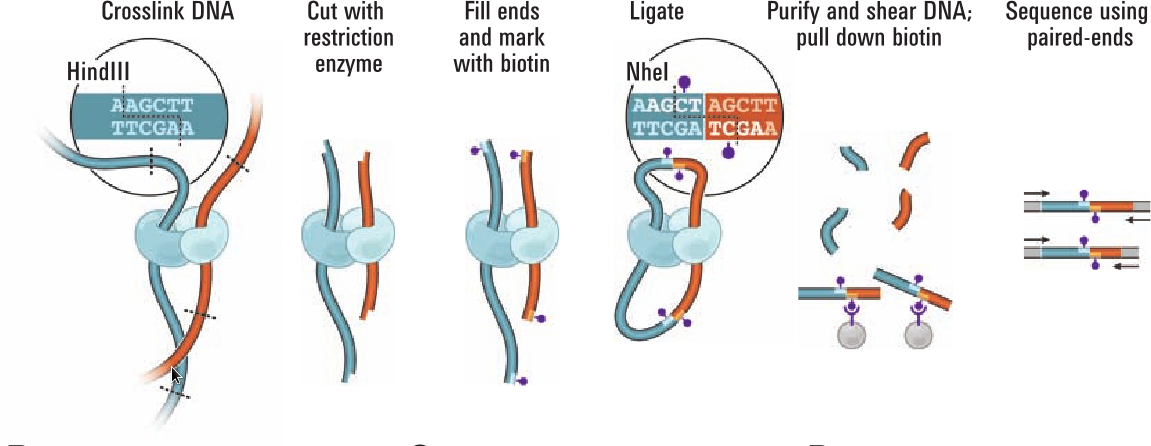
\includegraphics[width=0.8\linewidth]{figures/hic_protocol.png}
\end{center}
\caption{\textbf{Hi-C Protocol.} The procedure relies on cross linking,
restriction enzymes digestions, intra molecular ligation, deproteinization and
deep sequencing. Reads are then aligned to the reference genome, and binned at
$10kb$, $40bk$ or $100kb$ depending on coverage.}
\end{figure}


After paired-end sequencing, each pair of reads can be associated to one
\citep{lieberman-aiden:comprehensive} or several \citep{ay:identifying} DNA
interactions. We can then create a symmetric hollow matrix of integers, for
which entries correspond to the number of paired reads that fall into a bin.
We denote by $C$ the interaction frequency matrix, and $c_{ij}$ the
interaction frequency between locus $i$ and locus $j$.

These protocols are complex, and yield highly biased interaction frequencies
\citep{imakaev:iterative, cournac:normalization, yaffe:probabilistic}.
\citet{imakaev:iterative} proposes a simple iterative method, called ICE, to
normalize the data. In short, the authors assume that the bias of each entry
$c_{ij}$ of the matrix can be written as the product of two biases $\beta_i$
and $\beta_j$ corresponding to biases induced by loci. Hence, we can write
$c_{ij} = \beta_i \beta_j p_{ij}$, where $p_{ij}$ is the probability of locus
$i$ interacting with locus $j$. Thus, $\sum_i p_{ij} = 1$. This is a non convex
optimization problem that can be solved exactly by an iterative process. To
avoid degeneracies, we filter out the top 2\% sparse loci from our entry
matrix before applying ICE. To give an intuition, this method projects each
vector of interactions onto the $\ell_1$ unit ball. In practice, it yields an
expected interaction frequency count: $k p_{ij}$, where $k$ is the mean
interaction frequency.

Thought still quite recent, chromosome conformation capture and its genome
wide derivatives are now widely used to discover how DNA folds in a bunch of
different organisms \citep{duan:three, sexton:three-dimensional,
tanizawa:mapping, ay:three-dimensional}. The challenge is now to increase the
Hi-C resolution, using very large data sets with deeper sequencing
\citep{rao:3d, jin:high-resolution}. As any genome-wide sequencing data, Hi-C
usually requires several millions or billions of paired-end sequencing reads,
depending on genome size and on the desired resolution. Managing these data
thus requires optimized bioinformatics workflows able to extract the contact
frequencies in reasonable computational time and with reasonable storage
requirements. The overall strategy to analyze Hi-C data is converging among
recent studies and summarized in \cite{lajoie:hitchhiker}. Our collaborators
and we have built HiC-Pro, an an easy-to-use and complete pipeline to process
Hi-C data from raw sequencing reads to the normalized contact maps. Once these
processing steps are done, one can finally proceed to the study of genome
organization and DNA folding from Hi-C data in an attempt to unfold the
mysteries of genome architecture.

\section{The study of chromosome organization}

The study of chromosome organization based on contact counts maps broadly
falls into two categories: model-based studies and data-driven studies. The
former methods consider the polymer nature of DNA to leverage the theoretical
and computational work done in statistical physics of polymers to built with
as few assumptions as possible many chromosome conformations. Those chromosome
conformations are then used to compare against experimental data, such as Hi-C
contact counts matrices, in order to iteratively improve the models. These
models offer mechanistical insights into the folding of DNA. The latter
approaches use the experimental data to infer 3D models, by typically minizing
a cost function ensuring the models are as consistent as possible with the
data. These data driven models and analysis are the primary focus of this
thesis.

Though we here review some of the methods used to study and build models, this
is a very incomplete view of a blooming field. \citet{rosa:computational}
provide a more thorough (but again incomplete) overview of computational models
of genome architectures.

\subsection{DNA as a polymer}

Polymer physics divide homopolymers (polymers with identical monomers) into
three main types, which are then extended to build more complex models (1) the
\textit{random coil}, (2) the \textit{swollen coil}, (3) the
\textit{equilibrium polymer}. These polymers are characterized by
relationships such as the one between the size of a polymer subchain $L(s)$ as
a function of its lengths $s$, between the size of the polymer $L(N)$ and the
total length of this polymer $N$, or between the contact probability between
monomers $P(s)$ and the linear distance between monomers $s$. DNA being a
polymer, each pair of nucleic acid forms a monomer, and the distance $s$ is the
genomic distance between two loci.

The \textit{random coil} corresponds to an unconstrained polymer, best
described by a random walk. A \textit{random coil} of length $N$ has an
expected size of $N^{1/2}$, and so has any of its subchain: $L(s) \sim
s^{1/2}$. The contact probability between two monomers is $P(s) \sim
s^{-3/2}$. These relationships lead to a low density polymer, where contact
between monomers is sparse. The modeling of the \textit{random coil} does not
exclude the volume occupied by monomers: when taking in account that monomers
can not occupy the same chain, one obtains a new polymer model known as the
\textit{swollen coil}, best described as a self avoiding random walk. This
type of polymer occupies a larger space: $L(N) \sim N^{\frac{3}{5}}$.

\begin{figure}
\begin{center}
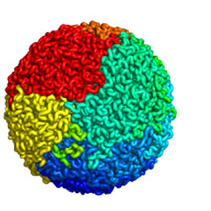
\includegraphics[width=0.8\linewidth]{figures/mirny_fractal.png}
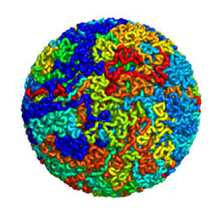
\includegraphics[width=0.8\linewidth]{figures/mirny_equilibrium.png}
\end{center}
\caption{\textbf{Fractal globule versus the equilibrium globule}}{This image
from \citet{mirny:fractal} illustrates the difference between the
\textit{fractal globule} or crumpled globule and the
\textit{equilibrium globule}. In the first row, the
fractal globule's subchain occupes a distinct territory in the nucleus, while
the second row illustrates the equilibrium globule's property to occupy a wide
space in the nucleus.}
\end{figure}

If the polymer is constrained in a small volume, the polymer folds into an
\textit{equilibrium globule} state. This polymer behaves as a random walk,
until it bounces of the boundary of the constrained space, and starts another
random walk inside the confined volume. The expected size of this polymer is
$N^{1/3}$. The size of a subchain of a polymer follows the relationship: $L(s) =
s^{1/2}$ for $s < N^{2/3}$ and constant elsewise: it is the same as a random
coil until it plateaus. The probability of contact between two monomers is
$P(s) = s^{-3/2}$ for $s < N^{2/3}$ and constant elsewise: once again, it is
the same relationship as the random coil, until it becomes constant.
Interestingly, this polymer is uniformely distributed in the constrained
space, and the density of the polymer is independent of the total length $N$
and the volume $V$.

Another interesting polymer behaviour is the \textit{fractal globule}: when
the chain is sufficiently long and the constrained volume sufficiently small,
the polymer forms knotted crumples of increasing sizes. The polymer is then
constrained by the available volume, and other parts of the polymer, which
creates topological constraints forcing the polymer to collapse into crumples.
First proposed by \citet{grosberg:role}, and further analysed by
\citet{mirny:fractal}, the polymer presents interesting properties: the size
of any subchain follows the same law as the equilibrium globule, but without
the plateau: $L(s) \sim s^{1/3}$, and the probability of contact between two
monomers is inversely proportional to the linear distance that separates them:
$P(s) \sim s^{-1}$.


\begin{figure}
\caption{{\bf FIXME} Relationship between contact counts and genomic distances}
\label{fig:hic_relationships}
\end{figure}

Now that we have briefly summarized the different theoritical behaviour of
polymers DNA can adopt, let us have a closer look at the relationships we
observe in the contact counts maps. We can observe that organism fall into two
categories: the first group, composed of small genomes such as \textit{S.
cerevisae}, \textit{P. falciparum}, behaves as an \textit{equilibrium globule}
coil, while the second group, composed of large genomes such as mammifer
genomes and \textit{A. thaliana} \textit{D. drosophilae}, exhibit properties
of \textit{fractal globules}.

\subsection{The inference of DNA three-dimensional models}


Several techniques have been developed to infer three-dimensional models of
the genome from interaction counts data. They fall into three categories: the
first finds an average structure by optimizing an objective function as
\citep{tanizawa:mapping, duan:three, ben-elazar:spatial}. The
second samples local minima from a optimization problem leading to the study
of the population of local minima \citep{bau:three-dimensional}. The last
samples the posterior distribution \citep{rousseau:three}.

\citet{tanizawa:mapping} model the 3D genome of the fission yeast (3
chromosomes) by a string of $622$ beads, each bead $x_i$ being the center of a
$20$kb section. The first step was to infer physical distances $\delta_{ij}$
from frequency interactions. They studied eighteen pairs of genes using FISH
measurements, and fitted the Hi-C data on the distances with a non linear
regression curve. The second step was to compute the coordinates of the beads,
such that the distances between the beads matches the inferred physical
distances to the best, with additional biological motivated constraints.

\citet{duan:three} converts the interaction frequencies into distances by
examining the relationship between interaction frequencies and genomic
distances. Then, a multidimensional scaling (MDS) is used to place each bead
so that the wish distances are respected as well as possible.

\citet{tanizawa:mapping} and \citet{duan:three} optimizes a problem of the
form:
\begin{equation*}
\renewcommand{\arraystretch}{2}
\begin{array}{ccll}
\underset{x_1,\ldots, x_n}{\text{minimize}} & &
\underset{i<j\leq n}{\sum} \big(\|x_i - x_j\|_2 - \delta_{ij}\big)^2 &\\
\text{subject to}
& & \text{biological motivated non convex constraints.}
\end{array}
\end{equation*}

\citet{tanizawa:mapping} published one solution, but did not mention the non
convexity of the problem. Hence, we assume they seeked the best local minimum
\citet{duan:three} ran the optimization process 30 times, and, observing the
obtained solutions, found that they did not differ much. No formal study was
done to compare the solutions.

\citet{lesne:3d} proposes a classical MDS algorithm \textit{ShRec3D} as follows:
(1.) construct a graph whose vertices are the loci assessed in the Hi-C
experiment, and the weights of vertices inversely proportional to the contact
counts (2.) compute a matrix of shortest path between pairs of loci which we
denote by the ``distance`` matrix (3.) apply a classical MDS on this distance
matrix. This yields a fast algorithm for inferring a consensus algorithm.

\citet{ben-elazar:spatial} formulated a non metric multidimensional scaling
optimization problem. They first filtered the interaction count matrix so that
remained only the most significant interactions. They then interpolated the
missing values to obtain a smooth, symmetric, positive definite matrix.

\citet{bau:three-dimensional} used IMP (Integrative Modeling Platform), also
used in nuclear magnetic resonance (NMR) microscopy to construct a 3D model of
the $\alpha$-globin module. Chromosomes are represented by beads, each beads
linked by restraining oscillators. IMP seeks a solution at the equilibrium of
those beads. Three types of restraints are used: the first  corresponds to
harmonic oscillators, with strengths inversely proportional to the 5C
score, computed from the interaction frequencies. The second ensures that two
beads cannot be too close to each other. The third ensure that two consecutive
beads cannot be separated too much. The last two springs have strength only
when the constraints are not fulfilled. The optimization of this problem
yields different configuration with similar IMP scores. A population of 50000
structures was computed. The 10000 structures with the smaller objective
function were then chosen as the population of local minima to be studied.

\citet{rousseau:three} and \citet{hu:bayesian} both describe a formal
probabilistic model of interaction frequencies and their relationship with
physical distances. They then use a Markov Chain Monte Carlo sampling
procedure to produce an ensemble of 3D structures consistant with the contact
count data.

\citet{tjong:physical} constructs a very simple model of the budding yeast
{\em S. cerevisiae} by modeling chromosomes
as a flexible fiber, and using additional biologically motivated constraints,
such as the positioning of centromeres and telomeres, they formulate an
optimization problem. Generating $200000$ feasible structures, they show that
Hi-C data can be fully explained by this very simple model.

\citet{wong:how} models the budding yeasts chromosomes a semi-flexible fiber
constrained in a nucleus, and applies 4 sequences specific forces on this
fiber to obtain certain properties: (1) centromeres are attached to a single
point of the nucleus by a segment; (2) telomeres are subjected to an outward
force, that pushes them towards the nuclear membrane; (3) rDNA is thicken; (4)
apply a random brownian movement. This models recovers many of the known
hallmarks of the 3D architecture of {\em S. cerevisiae}.

\citet{nagano:single-cell} and \citet{paulsen:manifold} both proposes methods
to infer 3D structures from single-cell Hi-C data. The first is a constraint
based modelisation: the structure is modeled as a flexible fiber as in
\citet{tjong:physical}, but beads are constraint to be in contact when an
interaction is observed in the single-cell contact map.
\citet{paulsen:manifold} formulates a \textit{manifold based optimization},
where a low rank psd matrix (and thus a distance matrix) is optimized to be as
close as possible to the sparse contact count matrix. Applying classical MDS
on this low rank psd matrix then yields a 3D model of the genome.

\begin{table}[ht!]
\caption{\bf A comparison of 3D inference methods}
\begin{center}
\small
\begin{tabular}{rlccccc}
\hline
\multirow{2}{*}{\emph{Publication}} & \multirow{2}{*}{\emph{Name}} &
\multirow{2}{*}{\emph{Consensus}} & \multirow{2}{*}{\emph{Population}}
&\multirow{2}{*}{\emph{MDS-based}} & \emph{Statistical} &
\multirow{2}{*}{\emph{Available}} \\
& & & & & \emph{model} & \\
\hline
\citet{duan:three} &  & x & & x & & x \\
\citet{tanizawa:mapping} & & x & & x & & \\
\citet{ay:three-dimensional} & & x & & x & & \\
\citet{ben-elazar:spatial} & & x & & x & & x \\
\citet{varoquaux:statistical} & Pastis & x & & & x & x\\
\citet{bau:three-dimensional} & & & x & & & \\
\citet{umbarger:three-dimensional} & & x & & & &\\
\citet{zhang:inference} & chromSDE & x & & x & & x\\
\citet{rousseau:three} & & & x & & x & x\\
\citet{hu:bayesian} & Bach & x & x & & x & x\\
\citet{kalhor:genome} & & & x & & &\\
%\citet{tokuda:dynamical} & & & & & &\\
\citet{wong:predictive} & & & x & & & \\
%\citet{gehlen:chromosome} & & & & & &\\
\citet{lesne:3d} & ShRec3D & x & & x & & x \\
\citet{trieu:large} & & x & & & & \\
\end{tabular}
\end{center}
\end{table}


\section{Long range interactions}


Thought mostly and initially used to study DNA folding, contact counts maps
have recently been re-purposed for diverse applications: \textit{de novo}
genome assembly \citep{burton:chromosome, kaplan:high-throughput},
deconvolution of metagenomic samples \citep{burton:species-level,
beitel:strain}, and genome annotation \citep{marie-nelly:filling,
varoquaux:accurate}.

\subsection{\textit{De novo} genome assembly, haplotype resolution and
metagenomic sample deconvolution}

\textit{De novo} genome assembly is the task of assembling many short DNA
reads into a whole genome. These short DNA reads can be assembled into short
contigs but the process of joining short contigs into larger scaffolds is
often made difficult due to the presence of repetitive sequences. Despite
improvements in sequencing technology and thus the sequencing of longer reads,
filling the gaps caused by these repetitive sequences in complex genome
remains difficult. \citet{burton:chromosome} and
\citet{kaplan:high-throughput} proposes to use the massive amount of DNA
sequences produced by Hi-C to first assemble short contigs, and rely on
contact counts informations between contigs to attempt to place them one
relatively to the other. Indeed, the more two contigs interact, the closer in
terms of genomic distances they should be (with the proper normalization in
contig lengths, GC-content, mappability and so on). The contact count matrix
of the ordered contigs (the "normal" contact count map) is simply a
permutation of rows and columns of the contact count matrix of the unordered
set of contigs. Assembling the genome can thus be seen as reordering rows and
columns to obtain a suitable Hi-C contact count matrix, smooth and with a
strong diagonal. \citet{burton:chromosome} proposes to first cluster contigs
into groups that belong to the same chromosomes, then create a graph where
each node is a contig, and vertex represents interactions of weight contact
counts. They then apply a minimum spanning tree algorithm to identify a path
in the graph corresponding to adjacent contigs. \citet{kaplan:high-throughput}
and \citet{marie-nelly:high-quality} both formulate the task as finding a
permutation of rows and columns to maximize a likelihood. As finding a
permutation matrix is a NP-hard problem, they use heuristic to simplify the
optimization problem.

Mammifer genomes contain two copies of each chromosomes, which themselves hold
specific single nucleotide polymorphisme (SNP). It is sometimes interesting to
identify whether SNPs or mutations are held on the same copy of the
chromosome. The task of identifying which SNP belongs to which chromosome is
known as resolving the haplotype. \citet{selvaraj:whole-genome}
proposes a very similar idea as
before, which is that reads containing SNPs on the same homologous chromosomes
interact more than SNPs on the other homologous chromosome. It is thus
possible to use contact count information between reads in order to determine
to which homologous chromosomes SNPs belong and resolve the haplotype.

Microbiomes contain an ensemble of very small organisms in different
abundances. Traditionnal technics to identify which organisms is in a
metagenomic sample rely on deep sequencing to produce millions of short DNA
reads. These reads are then either aligned on a reference genome or used as
input of a supervised learning algorithm (Kevin) to identify which organisms
are in the sample, and in which abundance. Both of these
methods need a priori knowledge of the community's composition. Recently,
\citet{burton:species-level} and \citet{marbouty:metagenomic} use shotgun
sequencing and Hi-C contact counts to determine which contigs belong to which
organisms. Once again, the idea is very similar as before: contigs from the
same organism interact amongst each other the most. Thus, a clustering
algorithm that takes as input a similarity matrix (the contact counts) groups
contigs from the same organism together. Once the organism's contigs are
identified, one can use technics as described before to scaffold contigs
together, and therefore in a single experiment do \textit{de novo} sequencing
of many organisms, and find the composition and abundance of a metagenomic
samples.

All these applications are based on a very simple and elegant idea that
contact counts map hold information on the contiguity of chromosomes which can
be leverage for various tasks.

\subsection{Genome annotations and centromeres identification}

The last unusual application of Hi-C data is the annotation of genomes, and
more specifically the detection of highly colocolized elements that are
elsewise difficult to annotate. In particular, centromeres have proven
difficult to precisely identify in many species, including highly studied and
used yeasts species. Centromeres, essential for proper chromosome segregation,
have the property of clustering in 3D, and thus have very specific signal
patterns in Hi-C data. \citet{marie-nelly:filling} proposed to annotate
centromeric regions by detecting these very specific patterns in the contact
maps of yeast species.

\section{Contributions of the thesis}

This thesis brings several contributions to the fields of analyzing Hi-C data.
We now review them, following the organization of the manuscript (and not in
chronological order of publication).

\begin{itemize}

\item Chapter \ref{chap:statistical} presents a novel, stable and robust
statistical method for inferring a consensus 3D model of the genome. We model
contact counts as a Poisson distribution where the 3D structure is a latent
variable, and formulate the inference problem as maximizing the likelihood. We
show both on generated and real Hi-C data that our method is more accurate,
stable and robust than previous methods. \footnote{Our method \textit{Pastis}
is available as a free and opensource software at
\url{http://cbio.ensmp.fr/pastis}}

\item Chapter \ref{chap:plasmodium} studies the 3D architecture of the
parasite {\em P. falciparum} during its erythrocytic cycle and its links with
gene expression. We assayed the genome architecture of the parasite at three
time points to obtain high resolution contact maps which we used to construct
consensus 3D models. The resulting models showed that {\em P. falciparum}'s
genome is folded in a complex architecture, that cannot be explained by a
simple volume exclusion model due to the strong co-clustering of many genomic
elements in the nucleus. We observe a strong link between chromatin structure
and gene expression, in particular reduced expression of genes located in
spatial proximity to the repressive subtelomeric center and colocalization of
distinct groups of parasite-specific genes with coordinated expression
profiles. Overall, our results show that the 3D structure of the parasite is
strongly correlated with gene expression during the erythrocytic cycle. This
work has been done in collaboration with Noble lab and Le Roch lab. My
contribution were (1) the 3D modeling of the genome using MDS-like approaches,
(2) the comparison to the volume exclusion modeling and (3) finding the link
between gene expression profiles and the 3D models using kernel CCA.

\item Chapter \ref{chap:centurion} presents work done while I was visiting
Noble lab, in collaboration with Dunham lab and Shendure lab. We proposed a
novel method to jointly identify yeasts centromeres from Hi-C data, using the
property centromeres have to strongly colocolize in the nucleus and thus to
create a specific pattern in the contact counts maps. Our method,
\textit{Centurion}, outperforms a previous published method by performing a
joint optimization and using a better strategy to initialize the optimization.
We show that \textit{Centurion} is very accurate and stable both on high and
low coverage datasets. \footnote{Our method \textit{Centurion} is available as
a free and opensource software at \url{http://cbio.ensmp.fr/centurion}}
\end{itemize}


% this file is called up by thesis.tex
% content in this file will be fed into the main document



\chapter[Inferring the 3D structure of the genome]{A statistical approach for inferring the 3D structure of the genome}
\graphicspath{{2_chapter/figures/}}

\begin{work}

This chapter has been published in a slightly modified form in
\citep{varoquaux:statistical} and presented at ISMB 2014, as joint work with
Ferhat Ay, Bill Noble and Jean-Philippe Vert.

\end{work}

% Résumé en francais

\begin{abstract}{Résumé}

Des récents développement dans les protocoles biologiques permettent désormais
de mesurer les fréquences d'interaction entre toutes les paires de loci d'un
génome, et ce en une seule experience. Le défi suivant est donc d'inférer des
modèles tri-dimensionnels du repliement des chromosomes dans
le noyau de la cellule. Les inférences proposées jusqu'à présent reposent
souvent sur des méthodes dites \textit{multidimensional scaling} (MDS),
lesquelles optimizent une structure telle que les distances relatives entre
éléments soient les plus proches de celles dérivées directement des fréquences
d'interaction. Ces approches optimizent une fonction objective heuristique,
et reposent sur de fortes hypothèses sur la biophysique de l'ADN pour trouver
la fonction de transfert entre fréquences d'interaction et distances
euclidiennes. Ces hypothèse peuvent donc conduire à l'inférence de modèles
incorrectes de la structure de l'ADN.

Dans ce travail, nous proposons une nouvelle méthode pour inférer une
structure 3D consensus du génome à partir de données Hi-C. Notre méthode
repose sur un modèle statistique des fréquences d'interaction. Nous modélisons
les fréquences d'interaction comme une distribution de Poisson dont
l'intensité dépends de la distance physique entre paires de loci. Notre
méthode peut automatiquement ajuster les paramètres de la fonction de
transfert entre fréquences d'interaction et distances physiques, et infère un
modèle expliquant au mieux les données.

Nous comparons deux variantes de notre méthode (avec ou sans optimization des
paramètres de la fonction de transfert) à quatre algorithmes utilisant MDS sur
des données simulées: deux MDS dit "métriques", dont les fonctions objectives
diffèrent, une version non métrique de cet algorithme, et ChromSDE qui propose
une version récente et convexe du MDS. Nous démontrons que notre modèle de
Poisson reconstruit des modèles plus précis que toutes les méthodes MDS, en
particulier lorsque la couverture des données est faible ou que les données
Hi-C sont à haute résolution, soulignant ainsi l'importance du choix de la
fonction objective à optimizer. Sur des données Hi-C publiques de cellules
embryoniquet de souris, nous démontrons par ailleurs que les méthodes Poisson
infèrent des structures plus stables, plus reproductibles et plus robustes à
la fois lorsque le protocole biologique diffère, mais aussi à différente
résolution.

Une implémentation Python de notre méthode est disponible à
\href{http://cbio.ensmp.fr/pastis}{http://cbio.ensmp.fr/pastis}.
\end{abstract}


\begin{abstract}{Abstract}
\textbf{Motivation:} Recent technological advances allow the
measurement, in a single Hi-C experiment, of the frequencies of
physical contacts among pairs of genomic loci at a genome-wide
scale. The next challenge is to infer, from the resulting DNA-DNA
contact maps, accurate three dimensional models of how chromosomes
fold and fit into the nucleus. Many existing
inference methods rely upon {\em multidimensional scaling} (MDS), in
which the pairwise distances of the inferred model are optimized to
resemble pairwise distances derived directly from the contact
counts. These approaches, however, often optimize a heuristic objective
function and require strong assumptions about the biophysics of
DNA to transform interaction frequencies to spatial distance, and thereby
may lead to incorrect structure reconstruction.

\textbf{Methods:}
We propose a novel approach to infer a consensus three-dimensional
structure of a genome from Hi-C data. The method incorporates a
statistical model of the contact counts, assuming that the counts
between two loci follow a Poisson distribution whose intensity decreases
with the physical distances between the loci. The method can automatically
adjust the transfer function relating the spatial distance to the Poisson
intensity and infer a genome structure that best explains the observed data.

\textbf{Results:}
We compare two variants of our Poisson method, with or without
optimization of the transfer function, to four different MDS-based
algorithms---two metric MDS methods using different stress functions,
a nonmetric version of MDS, and ChromSDE, a recently described, advanced
MDS method---on a wide range of simulated datasets. We demonstrate that the
Poisson models reconstruct better structures than all MDS-based methods,
particularly at low coverage and high resolution, and we highlight the
importance of optimizing the transfer function. On publicly available Hi-C data
from mouse embryonic stem cells, we show that the Poisson methods lead to more
reproducible structures than MDS-based methods when we use data generated using
different restriction enzymes, and when we reconstruct structures at different
resolutions.

\textbf{Availability:} A Python implementation of the proposed method
is available at \href{http://cbio.ensmp.fr/pastis}{http://cbio.ensmp.fr/pastis}.
\end{abstract}

\section{Introduction}

Spatial and temporal three-dimensional (3D) genome architecture is
thought to play an important role in many genomic functions, but is
still poorly understood \citep{vansteensel:genomics}. In recent years, the
technique of chromosome conformation capture (3C)
\citep{dekker:capturing}, which identifies physical contacts between
different genomic loci and yields information about their relative
spatial distance in the nucleus, has paved the way for the systematic
analysis of the 3D structure of DNA. Coupled with high-throughput
sequencing, genome-wide conformation capture assays, broadly referred
to as {\em Hi-C} \citep{lieberman-aiden:comprehensive}, have emerged
as promising techniques to investigate the global structure of DNA at
various resolutions. Hi-C has opened new avenues to understanding many
biological processes including gene regulation, DNA replication,
somatic copy number alterations and epigenetic changes
\citep{shen:map,ryba:evolutionarily, de:DNA, dixon:topological}.

A typical Hi-C experiment yields a DNA {\em contact map}, that is, a
matrix indicating the frequency of interactions between all pairs of
loci at a given resolution.  A fundamental question is then to
reconstruct the 3D structure of the genome from this contact map. Two
general approaches have been proposed for that purpose: (i)
\emph{consensus methods} that aim at inferring a unique mean structure
representative of the data and (ii) \emph{ensemble methods} that
yield a population of structures.

Consensus approaches \citep{duan:three,
  tanizawa:mapping, bau:three-dimensional} model each
chromosome by a chain of beads, convert the contact map frequencies
into pairwise distances (which we refer as \emph{wish
  distances}) using various biophysical models of DNA, and infer a 3D
conformation that best matches the pairwise distances by solving a
multidimensional scaling (MDS) problem
\citep{kruskal:multidimensional2}. Converting interaction counts to
physical wish distances requires, however, strong assumptions which
are not always met in practice. For example, this mapping may change
from one organism to another \citep{fudenberg:higher-order}, from one
resolution to another \citep{zhang:inference}, from one genomic distance 
range to another \citep{ay:statistical}, or from one time point to 
another during the cell cycle \citep{le:high-resolution, ay:three-dimensional}.

To alleviate this problem, \citet{zhang:inference} proposed ChromSDE,
a method that jointly optimizes the 3D structure and a parameter of
the function that maps contact frequencies to spatial distances, in
addition to modifying the objective function of MDS. \citet{ben-elazar:spatial}
proposed an approach akin to \emph{nonmetric MDS}
\citep{kruskal:multidimensional}, where the 3D structure and the wish
distances are alternatingly optimized in an attempt to preserve coherence
between the ranking of pairwise distances and the ranking of pairwise
contact frequencies.

As for the ensemble methods, \citet{rousseau:three} and
\citet{hu:bayesian} describe two formal probabilistic models of contact
frequencies and their relationship with physical distances. They then
use a Markov chain Monte Carlo (MCMC) sampling procedure to produce an
ensemble of 3D structures consistent with the observed contact counts.
\citet{kalhor:genome} propose an optimization framework that generates
a population of structures by enforcing each contact to define an active
constraint in only a fraction of the inferred structures, thereby mimicking the
heterogeneity of contacts coming from each cell in the Hi-C sample.
Applying a similar method to budding yeast, \citet{tjong:physical}
demonstrate that a large population of structures inferred using known
physical constraints of yeast genome architecture can recapitulate, to a
large extent, the consensus contact map observed from Hi-C experiments.

Both consensus and ensemble models have benefits and
limitations. Ensemble approaches are biologically more accurate,
because Hi-C data is derived from a population of cells, each with
potentially a unique 3D architecture. An inferred population of 3D
structures may therefore better reflect the diversity of structures
than a single consensus structure.  In concordance with such ensemble
methods, a recent development in Hi-C
technology, assaying chromatin conformation at a single cell level,
demonstrates that chromatin structure varies highly from cell to cell
by modeling the single-copy X chromosomes of a male mouse cell line
\citep{nagano:single-cell}.

However, an ensemble approach
raises the question of interpretability: one often has to fall back to
interpreting a mean signal from the population structure
\citep{kalhor:genome} or to selecting a few structures, representative
in some way of the diversity of the population
\citep{rousseau:three}.  Consensus
methods, in contrast, provide a single structure more amenable to
visual inspection and analysis.  This structure can be seen as a useful
\emph{model} to recapitulate the rich information captured in Hi-C data
and to allow easy integration with other sources of data, such as
RNA-seq, which are usually also population based. In addition, despite
the stochasticity of cell-to-cell variations, certain hallmarks
of genome organization observed by consensus methods, such as chromosome
territories or topological domain organization, are conserved across
different cells \citep{nagano:single-cell,hu:bayesian}.
Computationally, ensemble methods are more demanding than consensus methods
since they need to sample from a very large dimensional space of possible
structures with complicated likelihood landscapes. Optimization-based
consensus methods are usually faster to converge to a local optimum,
but may miss the global optimum corresponding to the best structure when
the objective function is non-convex.


In this work, we focus on the consensus approach, and we propose a new
method to infer a 3D structure from Hi-C data. We propose to
replace the arbitrary loss function minimized by existing MDS-based
approaches by a better-motivated likelihood function derived from a
statistical model, similar to the one use by a previous ensemble method \citep{hu:bayesian}.
Specifically, our proposed method models the interaction frequency between two
loci by a Poisson model (PM), the intensity of which decreases with the
increasing spatial distance between the pair of loci.
Similar to the problem of inferring the wish distances
from interaction frequencies faced by MDS-based approaches, our model
faces the difficulty of transforming spatial distances into
intensities of the Poisson distribution. To solve this problem,
we propose two variant methods. The first method (PM1) uses a default
transfer function motivated by a biophysical model, whereas the second
method (PM2) uses a parametric family of transfer functions, the parameters
of which are automatically optimized together with the 3D structure to best
explain the observed data.

We compare both PM variants to four MDS-based methods, including metric
MDS with two stress functions, nonmetric MDS and ChromSDE. We demonstrate
on simulated data that the new models reconstruct more accurate 3D structures
than all MDS-based methods, especially at low coverage and high resolution.
We also assess the negative effect of using an incorrect transfer function,
and we show that PM2 is able to overcome this difficulty. On real data, we show
that, compared to MDS-based methods, PM1 and PM2 generate more similar models
when applied to replicate experiments performed with different restriction enzymes
or when applied to the same data at varying resolutions. The results suggest that
the Poisson model methods we describe here provide promising alternatives to
current methods for consensus DNA structure inference.

\section{Approach}

We model chromosomes as series of beads in 3D, each bead representing
a genomic window of a given length, and we denote by $\Xb =
(x_1,\ldots,x_n) \in \RR^{3 \times n}$ the coordinate matrix of the
structure, where $n$ denotes the total number of beads in the genome
(for example, $n=1216$ at 10kb resolution for the yeast genome) and
$x_i\in\RR^3$ represents the 3D coordinate of the $i$-th bead. The Hi-C
data can be summarized as an $n$-by-$n$ matrix $\mathbf{c}$ in which
each row and column corresponds to a genomic locus, and each matrix
entry $c_{ij}$ is a number, called the {\em contact frequency} or {\em
  contact count}, indicating the number of times locus $i$ and $j$
were observed to contact one another. The matrix is by construction
square and symmetric.

\subsection{Data normalization}
The raw contact count matrix suffers from many biases, some technical (from
the sequencing and mapping) and others biological (inherent to the physical
properties of chromatin) \citep{yaffe:probabilistic, imakaev:iterative}.
Therefore, before inferring the 3D structure of the genome, we normalize each
raw contact matrix using iterative correction and eigenvalue decomposition
(ICE) \citep{imakaev:iterative}, a method based on the assumption that all
loci should interact equally. Due to mappability issues, some beads have zero
contact counts. We remove these beads from the optimization and only try to
infer the positions of beads with nonzero contact counts.


\subsection{MDS-based methods}

\subsubsection{Metric MDS}

Metric MDS is a classical method to infer coordinates of points given their
approximate pairwise Euclidean distances~\citep{kruskal:multidimensional2}. To
use MDS in the context of DNA structure inference from Hi-C data, we need to
assign each pair of beads ($i$, $j$) a physical wish distance
$\delta_{ij}$---i.e., the distance that we aim to capture with our 3D
model---derived from the bead pair's contact count $c_{ij}$. Performing this
assignment requires us to decide how contact counts are transformed into physical
distances. In Section~\ref{sec:evaluating_parameters} we discuss a commonly used
transformation of the form $\delta_{ij} = \gamma
c_{ij}^{-3}$ if $c_{ij}>0$ motivated by polymer physics.
Metric MDS then places all the beads in 3D space such that
the Euclidean distance $d_{ij}(\Xb) = \|x_i - x_j\|$ between the beads $i$ and
$j$ is as close as possible to the wish distance $\delta_{ij}$. Denoting by
$\Dcal$ the subset of indices whose distances we wish to constrain (typically,
the set of pairs $(i,j)$ with non-zero contact counts $c_{ij}>0$), metric MDS
attempts to minimize the following objective function, usually called the \emph{raw
stress}:
\begin{equation}\label{eq:mds1}
\renewcommand{\arraystretch}{2}
\begin{array}{ccll}
\underset{\mathbf{X}}{\text{minimize}} & &
\underset{(i,j) \in \mathcal{D}}{\sum} \big(d_{ij}(\Xb) - \delta_{ij}\big)^2 \,.&\\
\end{array}
\end{equation}

In two previous studies that use metric MDS,
\citet{duan:three} and \citet{tanizawa:mapping} infer the 3D structure of DNA
from Hi-C data by solving Equation \ref{eq:mds1}, limiting $\Dcal$ to pairs of
indices with statistically significant contact counts (FDR 0.01\%). Both methods use
additional constraints such as
minimum and maximum distances between adjacent beads, minimum pairwise
distances between arbitrary beads to avoid clashes, and organism-specific constraints that concern the
positioning of centromeres, telomeres and ribosomal RNA coding regions. In
the experiments we present here, we simply solve Equation~\ref{eq:mds1} without
any constraints but including all pairs of beads with positive counts in $\Dcal$, and we call the
resulting method MDS1. In general, we have observed that
adding constraints related to minimal and maximal distances between beads
is unnecessary, because the structures found by MDS1 typically fulfill all of these constraints (data not shown).

A drawback of the raw stress of Equation~\ref{eq:mds1} in our context is that the
quadratic form is dominated by large values, corresponding to pairs of loci
with large wish distances (i.e., small contact counts). Because these counts are
less reliable than large contact counts, we propose a variant of MDS1, which
we call MDS2, where we weight the contribution of a pair $(i,j)$ in the stress
by a factor inversely proportional to the square wish distance between the corresponding
beads:
\begin{equation}\label{eq:mds2}
\renewcommand{\arraystretch}{2}
\begin{array}{ccll}
\underset{\mathbf{X}}{\text{minimize}} & &
\underset{(i,j) \in \mathcal{D}}{\sum} \delta_{ij}^{-2} \big(d_{ij}(\Xb) - \delta_{ij}\big)^2 \,.&\\
\end{array}
\end{equation}
While other weighting schemes could be proposed to decrease the influence of
pairs with large wish distances, we found this formulation to be quite robust
in practice. Notice that MDS2 can be thought of as a quadratic approximation of
the raw stress (minimized by MDS1) applied to log-transformed distances, because
in the setting $d_{ij}(\Xb) \approx \delta_{ij}$ it holds that:
\begin{equation*}
\begin{split}
\sum_{(i,j) \in \mathcal{D}} \br{\log d_{ij}(\Xb) - \log \delta_{ij}}^2
& = \sum_{(i,j) \in \mathcal{D}} \log\br{\frac{d_{ij}(\Xb)}{\delta_{ij}}}^2 \\
& \approx \sum_{(i,j) \in \mathcal{D}} \br{ \frac{d_{ij}(\Xb)}{\delta_{ij}}-1}^2 \,.
\end{split}
\end{equation*}
Both MDS1 and MDS2 implicitly
ignore non-interacting pairs of beads (i.e., pairs with zero contact
counts).

In addition to MDS1 and MDS2, we include in our benchmark ChromSDE
\citep{zhang:inference}, a recently proposed method which also attempts to
minimize a weighted stress function penalized by an additional term to push
non-interacting pairs far from each other. In addition, ChromSDE optimizes the
exponent of the transfer function that maps from contact counts to
wish distances. However, it
does not infer the relative positions of chromosomes. Accordingly, we compare
only the reconstruction of each individual chromosome produced by each method. Note
that, because intra-chromosomal counts are more reliable than inter-chromosomal
counts, ChromSDE should not be penalized compared to the other methods by
only considering intra-chromosomal counts.

\subsubsection{Nonmetric MDS (NMDS)}
\label{sec:nmds}

The derivation of the transfer function from contact counts to 3D wish distances, 
needed by metric MDS-based methods, relies on strong
assumptions about the physics of DNA
(Section~\ref{sec:evaluating_parameters}). NMDS \citep{shepard:analysis,kruskal:multidimensional} offers an alternative 
way to proceed, which was proposed in the context of DNA structure inference 
from Hi-C data by \citet{ben-elazar:spatial}. Instead of inferring physical
distances from the contact matrices, NMDS relies on the sole
hypothesis that if two loci $i$ and $j$ are observed to be in contact more
often than loci $k$ and $\ell$, then $i$ and $j$ should be closer in 3D space
than $k$ and $\ell$.  Using this hypothesis, NMDS attempts to solve the
following problem:
\begin{problem}
Given a set of similarities $c_{ij}$ (e.g., the contact frequency between $i$ and $j$), find 
$\mathbf{X} \in R^{3 \times n}$ such that:
\begin{equation}
\label{eq:ordinal_constraint}
c_{ij} \geq c_{k\ell} \Leftrightarrow \|x_i - x_j\|_2 \leq \|x_k -
x_\ell\|_2 \,.
\end{equation}
\end{problem}
Equation~\ref{eq:ordinal_constraint} is known as the nonmetric
constraint, or the ordinal constraint. This problem was first introduced
by \citet{shepard:analysis} and formalized as an optimization problem
by \citet{kruskal:multidimensional}. It can be solved by minimizing the
cost function:
\begin{equation}
\underset{\mathbf{X,\Theta}}{\text{minimize}}
\  \sum_{i, j} \frac{\br{\|x_i - x_j\|_2 -
\Theta(c_{ij})}^2}{\Theta(c_{ij})^2},
\end{equation}
with respect to the embedding $\mathbf{X}$ and the function $\Theta$,
where $\Theta$ is a decreasing function. Algorithms to solve this
optimization problem involve iterating over two steps: (1) fixing
$\Theta$ and minimizing the objective function with respect to $\mathbf{X}$ (hence falling
back to solve MDS2), and (2) fitting $\Theta$ to the
new configuration $\mathbf{X}$ subject to the ordinal
constraints. This second step of the algorithm can be performed using an
isotonic regression method, such as the pool adjacent violator
algorithm \citep{best:minimizing}.

A trivial solution of this problem is to set $\Theta$ equal to
$0$. In this case all points will collapse on the origin. To avoid this collapse,
we add additional constraints on $\mathbf{X}$ or on
$\Theta$, such as $\sum_{i, j} \|x_i - x_j\|_2 = K$ for some constant
value of $K$.

\subsection{Poisson model}
\label{sec:pm}

Instead of metric or non metric MDS-based methods, which attempt to minimize a stress function that measures a discrepancy between the wish distances and the 3D distances of the structure, we propose to cast the problem of structure inference as a maximum likelihood problem. For that purpose, we need to define a probabilistic model of contact counts parametrized by the 3D structure that we want to infer from contact count observations.

For that purpose, we take a model similar to the one used in the BACH algorithm~\citep{hu:bayesian} and model the contact frequencies $(c_{ij})_{(i,j)\in\Dcal}$ as independent Poisson random variables, where the Poisson parameter of $c_{ij}$ is a decreasing function of $d_{ij}(\Xb)$ of the form $\beta d_{ij}(\Xb)^\alpha$, for some parameters $\beta>0$ and $\alpha<0$.
We can then express
the likelihood as
\[
\ell(\mathbf{X}, \alpha, \beta) =
  \prod_{i, j} \frac{(\beta d_{ij}^{\alpha})^{c_{ij}}}{c_{ij}!}
	\exp (- \beta d_{ij}^{\alpha})\,.
\]
By maximizing the log likelihood, a new optimization problem naturally
emerges from this formulation:
\begin{equation}
\renewcommand{\arraystretch}{2}
\begin{array}{cll}
\underset{\alpha, \beta, \textbf{X}}{\text{max}} &
\mathcal{L}(\mathbf{X}, \alpha, \beta) = \underset{i<j\leq n}{\sum}  c_{ij}
\alpha \log d_{ij} + c_{ij} \log \beta - \beta d_{ij}^\alpha &\\
\end{array}
\end{equation}
With this new formulation, we can either provide the parameter $\alpha$, using
prior knowledge, and only optimize the structure and $\beta$ (which depends on
the dataset), or we can use a nonmetric approach, by inferring $\alpha$.
We refer to the former as PM1 and to the latter as PM2.

PM2 is solved using a coordinate-descent algorithm:
first choose randomly an $\mathbf{X}$ configuration, then iterate
between maximizing $\mathcal{L}$ with respect to $\alpha$ and $\beta$
 and, fixing $\alpha$ and $\beta$ and maximizing $\mathcal{L}$
with respect to $\mathbf{X}$.  In this work, we try to
initialize $\textbf{X}$ with a good approximation of the solution by
first evaluating the parameters $\alpha$ and $\beta$ using some prior
knowledge and initialize $\textbf{X}$ with the inferred structure from
the MDS.

%\begin{equation}
%\frac{\partial \mathcal{L}}{\partial{\alpha}}(\alpha, \beta, \textbf{X}) =
%  \sum_{i, j \in \mathcal{D}} c_{ij} \log d_{ij} - \beta  d_{ij}^{\alpha} \log d_{ij}
%\end{equation}

%\todo{If space allows, we could write some more equations, like the minimum in $\beta$ or the gradients.}
%\todo{We should change the name EM (expectation-minimization) because what we do is quite different from standard EM. In standard EM, one would model observed data (count matrix C) and hidden variable (X) through a parametric model $P_a(C,X)$. To optimize the parameter a, one would first perform a E step where we would compute $E_a(X|C)$ , and then adjust the parameters. What we do is not computing the expectation of the structure, but instead the best structure (that maximizes $P_a(X|C)$, assuming a uniform prior on X) before reoptimizing the weights. To make a comparison with a more classical model, it is as if for hidden markov models we would run a Viterbi to find the most likely hidden variables, then optimize the parameters to maximize the likelihood of the hidden variables, as opposed to the EM approach (Baum-Welsh) where instead of Viterbi we need to estimate the expectation of the hidden variables. Mathematically, the EM procedure ensures that the likelihood of the observations observe, while what we do does not. By the way, a real EM may be relevant, in fact it would probably involve sampling a family of structures (as in the population methods), then do the average distances over the populations and optimize the parameters on that (details to be checked...).}

All optimization problems (MDS1, MDS2, NMDS, PM1 and PM2) were solved using IPOPT, an interior point filter
algorithm \citep{wachter:on} and the isotonic regression implementation from
the Python toolbox Scikit-Learn for NMDS \citep{pedegrosa:scikit}.


\subsection{Default contact-to-distance transfer function}
\label{sec:evaluating_parameters}

A prerequisite for both the MDS and the PM1 model (and for good initialization
of the NMDS and PM2 methods) is a function that converts from contact counts
to wish distances.  Extensive previous studies of the behaviour of polymers in
general and DNA in particular have yielded proposed relationships between, on
the one hand, the genomic distance $s$ and contact counts $c$ and, on the
other hand, genomic distance $s$ and physical distances $d$ for several
classes of polymers \citep{grosberg:role, lieberman-aiden:comprehensive,
fudenberg:higher-order}. For a fractal globule polymer, representative of
mammalian DNA, the contact count is inversely proportional to the genomic
distance ($c \sim s ^{-1}$), whereas the volume scales linearly with the
subchain length ($d^3 \sim s$), from which we deduce a relationship between
$d$ and $c$ of the form $d \sim c ^{-1/3}$. For an equilibrium globule,
representative of a smaller genome such as {\em S.\ cerevisae}, the
relationships differ: $c \sim s ^{-3/2}$ and $d \sim s ^ {1 / 2}$ up to a
maximum distance, corresponding to the size of the nucleus in which the DNA is
confined. Conveniently, coupling those two relationships for either type of
polymer yields the same mapping between contact counts and physical distances:
\begin{equation}
d \sim c ^{-1/3}.
\end{equation}
Thus, by default we convert contact counts $c_{ij}$ into 3D wish distances
$\delta_{ij}$ using the following relationship:
\begin{equation}
\delta_{ij} = \gamma c_{ij} ^{-1/3},
\end{equation}
where $\gamma$ defines the scale of the structure. It is important to note that 
this relationship holds true for only a subset of the full genomic distance range and
that this range varies for different genomes. In practice, we will not
infer $\gamma$ for the MDS and NMDS problem: the structures can easily be
rescaled after convergence to match biological knowledge of the organism
studied.

\subsection{Data}
\label{sec:data}

In order to test various 3D architecture inference methods, we
conducted experiments on both simulated datasets and publicly
available genome-wide Hi-C datasets.

For the simulation, we generated 170 data sets using the yeast genome
architecture proposed by \citet{duan:three}. Because the repetitive
rDNA on yeast chromosome XII cannot be observed in practice, we
discard all contacts involving these loci, and we do not infer the
position of the corresponding rDNA. We generate these 170 datasets
using the following model:
\begin{equation}\label{eq:simu}
c_{ij} = P(\beta d_{ij}^\alpha),
\end{equation}
where $\alpha = -3$ (corresponding to the theoretical exponent discussed in Section~\ref{sec:evaluating_parameters})
and $\beta$ varies between $0.01$ and $0.7$ ($0.01$, $0.01$, $0.02$, $0.03$,
$0.04$, $0.05$,
$0.06$, $0.07$, $0.08$, $0.09$, $0.1$, $0.15$, $0.2$, $0.3$, $0.4$, $0.5$, $0.6$,
$0.7$) with 10
different random generator seeds, thus obtaining 10 different datasets per
parameter.
The $\beta$ parameter controls the number of contact counts in the
datasets. A low $\beta$ will yield a dataset with few counts; hence, the
corresponding wish distance matrix will be less likely to be close to the true
distance matrix. To estimate how noisy the generated data is, we compute the
following measure of signal-to-noise ratio (SNR):
\begin{equation}
SNR = \frac{\sum{c_{ij}}}{\sqrt{\sum (\beta d_{ij} ^{\alpha} - c_{ij})^2}}\,.
\end{equation}
The numerator (the signal) corresponds to the number of counts, and
the denominator (the noise) corresponds to the sum of deviation
between each count and its expected value.  We use this first ensemble
of simulated datasets to assess the robustness to noise of the
different methods. Note that in actual data, the SNR gets smaller when we sequence fewer reads or when we infer a structure at a higher resolution.

We simulated another ensemble of datasets to compare nonmetric and metric
methods when the parameters provided to the different algorithms are not
the correct ones. We generate 20 datasets according to
Equation~\ref{eq:simu}, with $\alpha$ between $-4$ and $-2$ ($-4$, $-3.5$,
$-3$, $-2.5$, $-2$) and $\beta$ between
$0.4$ and $0.7$ ($0.4$, $0.5$, $0.6$, $0.7$).

We also applied our methods to publicly available Hi-C data from mouse
embryonic stem cells (mESC) \citep{dixon:topological}.  We started with the
data at 20~kb resolution and considered only chromosomes 1 to 19, with both
available restriction enzymes (HindIII and NcoI).  We then subsampled the data
at resolutions of 100~kb, 200~kb, 500~kb and 1~Mb.
Note that the methods studied here infer a single copy per
chromosomes, thus yielding a consensus model for both homologous chromosomes.


\subsection{Structure similarity measures}
In order to assess the ability of a method to reconstruct a known
structure from simulated data, or the stability of the reconstructed structure with respect to change in resolution or library preparation, we need quantitative measures of similarity between 3D structure. We use two such measures: the root mean square deviation (RMSD) and the distance error, which we now explain.

The RMSD is a
standard way to compare two sets of structures described by their
coordinates $\mathbf{X}, \mathbf{X}' \in R^{3 \times n}$, widely used for example to compare protein 3D structures. It is given by:
\begin{equation*}
RMSD = \min_{\mathbf{X}^*} \sqrt{\sum_{i = 1}^n (\mathbf{X}_{i} -
  \mathbf{X}_{i}^*)^2} \,,
\end{equation*}
where the structure $\mathbf{X}^*$ is obtained by translating,
rotating and rescaling $\mathbf{X}'$ ($\mathbf{X}^* = s \mathbf{R X'} -
\mathbf{t}$, where $\mathbf{R} \in R^{3 \times 3}$ is a rotation
matrix, $\mathbf{t} \in R^{3}$ is a translation vector, and $s$ is a
scaling factor). Because ChromSDE
does not infer the relative position of chromosomes, the RMSD values we report below
are sums of RMSDs computed independently on each chromosome.

We also directly compare the 3D distance matrices corresponding to the two structures with the distance error:
\begin{equation*}
\text{distanceError} = \sqrt{\sum_{i, j = 0}^n (d_{ij}(\Xb) - d_{i, j}(\Xb'))^2} \,.
\end{equation*}


The main difference between the optimization formulated by ChromSDE
and those of the other methods is the penalty assigned to
non-interacting beads.  Due to this penalty, ChromSDE should recover
better long distances than other MDS-based methods.  This property is
not well captured by the RMSD measure, therefore, we also compute how
well the distance matrix is recovered with the distance error, which assigns most of the weight to long distances. We
expect that methods based on MDS, which optimize an objective function
based on the distance matrix, should perform better on this measure
than others.

\section{Results}

To assess the relative strength of our new Poisson model-based methods, PM1 and PM2, we compare them to a panel of four MDS-based methods: MDS1, MDS2, NMDS and ChromSDE on simulated and real data.

\subsection{Simulated Hi-C data}

We first tested the six methods on data simulated as explained in Section~\ref{sec:data}.

\begin{figure}
\includegraphics[width=\linewidth]{{varoquaux.78.fig1}.pdf}
\caption{\textbf{Performance evaluation on simulated data, varying the parameter $\beta$.}
\textbf{A} RMSD of each experiment for varying values of the parameter $\beta$. ChromSDE
failed to yield consistent results for 14 experiments (It reported the wrong number of beads
in the results file.), and the PM2 algorithm
failed to converge at the desired precision for one experiment (It exceeded the
maximum number of iterations.).
\textbf{B} Distance error of each experiment for varying values of $\beta$.
\textbf{C} Average SNR for each $\beta$. Higher SNR corresponds to better quality data.
}
\label{fig:generated_data}
\end{figure}

\subsubsection{Performance as a function of SNR}

We ran all six methods---MDS1, MDS2, NMDS, PM1, PM2 and ChromSDE---on the 170
simulated datasets with varying SNR levels. Our goal here is to assess how
well the different methods manage to reconstruct a known 3D structure from
simulated data at different SNR levels. Remember that SNR estimates how far
the empirical counts differ from their expectations; in real Hi-C data, SNR
typically decreases when we have fewer reads in total, or when we want to
increase the resolution of the structure. In this first series of experiments,
we provide the correct count-to-distance or distance-to-count transfer
functions to the methods that need them (MDS1, MDS2, PM1). In this setting,
for infinite SNR, all methods should consistently estimate the correct
structure.

Figure~\ref{fig:generated_data} shows the performance of the different methods
in terms of RMSD (top) and distance error (middle) as a function of the
$\beta$ parameter, which controls the SNR (bottom). As expected, all methods
perform well when the SNR is high, but exhibit marked differences in
performance for finite SNR. In the low SNR setting (SNR $< 2$), both PM1 and
PM2 significantly outperform all MDS-based methods, in both RMSD and distance
error. Interestingly, we observe no significant difference between PM1 and
PM2, which shows that there is no price to pay in terms of inferred structure
if we don't specify the exponent of the distance-to-count transfer function.
In this setting, PM2 is able to estimate the structure accurately enough to
produce a structure of the same quality as PM1. Among MDS-based methods, we
see that NMDS generally outperforms MDS2, which itself outperforms MDS1. This
observation highlights that in the non-asymptotic, low SNR setting, the choice
of stress function influences the performance of MDS. ChromSDE performs better
than other MDS-based methods on datasets with a low SNR, corresponding to
datasets with low coverage and, consequently, many non-interacting pairs of
beads. This may be due to the way ChromSDE explicitly handles such pairs. On
the other hand, in a more favorable setting (SNR $>2$), ChromSDE does not
perform as well as other MDS-based method; we hypothesize that when the
coverage is high enough, taking into account non-interacting pairs of beads
does not add any additional information. Since ChromSDE is not better than
other MDS-based methods, and requires much longer to run, we do not report its
performance on the next experiments and instead focus on the differences
between the other MDS-based methods and the PM methods.

\subsubsection{Metric versus nonmetric methods: robustness to incorrect parameter estimation}

\begin{figure}
\includegraphics[width=\linewidth]{{varoquaux.78.fig2}.pdf}
\caption{\textbf{Performance evaluation for simulated data, varying
    the parameter $\alpha$.} The figure plots the average RMSD of the
  inferred structures for a range of $\alpha$ values.  As $\alpha$
  increases, the SNR of the dataset also increases.}
\label{fig:rmsd_alpha}
\end{figure}

Three of the methods tested, which we collectively refer to as \emph{metric}
methods, require as input a count-to-distance or distance-to-count transfer
function: MDS1, MDS2 and PM1. In reality, however, the DNA may not follow the
ideal physical laws underlying the default transfer function discussed in
Section~\ref{sec:evaluating_parameters}, and the structures inferred from
these methods may diverge from the correct one because of miss-specification
of the transfer function.

To assess this phenomenon, and evaluate the robustness of the different
methods (including NMDS and PM2, which automatically infer a transfer
function), we now study the performance of the methods on datasets generated
with varying $\alpha$ parameters. We therefore run the MDS1, MDS2, NMDS, PM1
and PM2 methods on the second ensemble of simulated datasets. We provide the
default transfer function to all metric methods, thus inducing a
miss-specification for all simulated datasets with $\alpha\neq -3$.

Figure~\ref{fig:rmsd_alpha} shows the RMSD of each method, averaged
over the datasets with different $\beta$, as a function of $\alpha$.
The performance curve of PM1, which is the best method when the data
are simulated with the correct parameter $\alpha=-3$, exhibits a
characteristic U-shape centered around $\alpha = -3$. This curve
confirms that PM1 performs better when given the true parameter and
performs worse as $\alpha$ moves away from $-3$. On the other hand,
the performance curves of the two other metric methods, MDS1 and MDS2,
do not exactly follow this trend: MDS1 and NMDS perform increasingly
better when $\alpha$ decreases, and MDS2 achieves the best performance
when $\alpha = -3.5$. This phenomenon occurs because in our
simulation, when $\alpha$ decreases, the SNR for a given $\beta$
increases, counterbalancing the negative effect of the transfer
function miss-specification.  Thus, for MDS-based methods, it is
apparently more important to have more data than to have a correct
$\alpha$ parameter. Finally, we see that, as expected, the non-metric
approaches, NMDS and PM2, are more robust to transfer function
misspecification than the metric approaches, because they
automatically estimate it. When the parameter is wrong, PM2
outperforms the other methods for low SNR, whereas for high SNR, NMDS
performs better.

\subsection{Real Hi-C data}

We now test the different methods on real Hi-C data. Since in this case the
true consensus structure is unknown, we investigate the behaviors of the
different methods in terms of their ability to infer consistent structures
from different datasets and across resolutions.

\begin{table*}
\begin{center}
\footnotesize
\begin{tabular}{ccccccccccccc}
\hline
{\tiny Resolution} &  Corr &
\multicolumn{2}{c}{MDS1} &
\multicolumn{2}{c}{MDS2} &
\multicolumn{2}{c}{NMDS} &
\multicolumn{2}{c}{PM1} &
\multicolumn{2}{c}{PM2} \\
&& {\tiny RMSD} & Corr & {\tiny RMSD} & Corr & {\tiny RMSD} &Corr & {\tiny
RMSD} & Corr & {\tiny RMSD} & Corr \\
\hline
1~Mb  & 0.981 & 13.13 & 0.945 & 5.54 & 0.964 &  5.80 & 0.965 & 7.28  & 0.931 & \textbf{4.92} & \textbf{0.976} \\
500~kb & 0.959 & 10.00 & 0.942 & 5.68 & 0.959 & 5.67 & 0.959 & 7.14 & 0.913 & \textbf{4.66} & \textbf{0.968} \\
200~kb & 0.845 & 5.64 & 0.940 & 3.74 & 0.945 & 3.73 & 0.946 & 4.01 & 0.891 & \textbf{3.42} & \textbf{0.958} \\
100~kb &  0.605 & 5.07 & 0.736 & 2.53  & 0.676 & 2.52 & 0.666 & \textbf{2.51} & 0.664 & 2.76 & \textbf{0.771}\\
\hline
\end{tabular}
\end{center}

\caption{\textbf{Stability across enzyme replicates.} For each resolution, the
table lists the Spearman
correlation the two enzyme replicate datasets, and, for each inference
method, the average RMSD and Spearman correlation between pairs of structures
inferred from the two datasets.  Boldface values correspond to the best RMSD
or correlation values among all five methods.  In general, higher resolution
leads to a lower correlation between pairs of inferred structures.}

\label{table:results_real_data}
\end{table*}
\subsubsection{Stability to enzyme replicates}

The Hi-C assay depends upon a restriction enzyme to cleave the DNA after
cross-linking, and the same sequence library can be analyzed multiple times
using different enzymes.  Although the resulting restriction fragments will
differ, we expect {\em a priori} that the overall genome architecture should
be the same from such replicate experiments.  We therefore evaluate each
genome architecture inference method with respect to the similarity of the
structures inferred from two replicate Hi-C experiments that differ only in
the choice of restriction enzyme.  Specifically, we apply each method to two
enzyme replicates, HindIII and NcoI, carried out in mouse ES cells
\citep{dixon:topological} for chromosomes 1--19.

To measure the stability of the methods, we compute (1) the Spearman
correlation between the two pairwise Euclidean distance matrices of
the pairs of predicted structures and (2) the RMSD between the
rescaled predicted structures.  Note that, before computing our two
error measures, we filter out from the pair of structures any beads
for which the inference hasn't been done on either dataset, i.e.,
beads that have zero contact counts in either data set.

To give a sense of how similar the two replicate datasets are, we also
compute the Spearman correlation directly on the data, rather than on
the inferred structures.  As expected
(Table~\ref{table:results_real_data}), the higher the resolution is,
the lower the correlation between the pairs of datasets is and the
more different the inferred structures are.
Across different enzyme replicates, the PM2 method yielded significantly
higher correlation than all of the other methods ($p < 0.05$,
signed-rank test
adjusted for multiple tests with a Bonferroni correction).



\subsubsection{Stability to resolution}

\begin{table}
\begin{center}
\begin{tabular}{clllll}
\hline
   & MDS1 & MDS2 & NMDS & PM1 & PM2 \\
\hline
{\em RMSD }        & 14.86 & 12.92 & 12.98 & 13.03 & \textbf{11.48} \\
{\em Correlation } &  0.781 & 0.754 & 0.738 & 0.737 & \textbf{0.807} \\
\hline
\end{tabular}
\end{center}
\caption{\textbf{Stability across resolution.} The table lists the
  average RMSD and Spearman correlation between pairs of structures of
  different resolutions. In bold are the lowest average RMSD and
  highest average Spearman correlation. These values were computed on
  mouse ESC HindIII libraries \cite{dixon:topological})}
\label{table:real_hic_stability}
\end{table}

\begin{figure*}
\begin{center}
\includegraphics[width=0.9\linewidth]{{varoquaux.78.fig3}.png}
\end{center}
\caption{\textbf{Predicted structures for chromosome 1 at different resolution}
Contact counts matrices and predicted
structures for the MDS2, NMDS, PM1 and PM2 methods at 1~Mb (\textbf{A}),
 500~kb (\textbf{B}), 200~kb (\textbf{C}),
100~kb (\textbf{D})}
\label{fig:real_data}
\end{figure*}

\citet{zhang:spatial} show that the mapping from contact counts to
physical distance differs from one resolution to another, underscoring
the importance of good parameter estimation. To study the stability of
the structure inference methods to changes in resolution, we compute
the RMSD between pairs of structures inferred at different
resolutions.  Let $(\textbf{X}, \textbf{Y}) \in (R^{3 \times n}, R^{3
  \times m})$ be a pair of predicted structures such that $n < m$
(i.e., $\textbf{X}$ is a structure at a lower resolution than
$\textbf{Y}$). We compute a downsampled structure $\textbf{Y}^* \in
X^{3 \times n}$ at the same resolution as $\textbf{X}$ by averaging
the coordinates of beads.  We then compute the RMSD between this new
structure $\textbf{Y}^*$ and $\textbf{X}$, as well as a corresponding
Spearman correlation of the distance matrices.

Results are shown in Figure~\ref{fig:real_data} and
Table~\ref{table:real_hic_stability}. PM2 is significantly ($p < 0.05$)
more stable to resolution changes, both in terms of RMSD and correlation of
distances.

\section{Discussion and conclusion}

In this work, we present a novel method for inferring a consensus genomic 3D
structure from Hi-C data. The method maximizes a likelihood derived from a
statistical model of the relationship between the contact counts and physical
distances, and includes an automatic tuning of the parameters defining the
link between a 3D distance and the Poisson parameter of the corresponding
contact count. We showed in simulations that the new method outperforms a
panel of MDS-based approaches, including ChromSDE, which optimize an often
ad-hoc stress function. The improvement is particularly important at low SNR,
corresponding to more difficult problems where we want to increase the
resolution of the model with a fixed total number of reads; this is typically
the situation where one expects a correct maximum likelihood estimator to
outperform more {\em ad hoc} estimators. We also showed that misspecification
in the count-to-distance transfer function can harm the performance of metric
methods, while our model can adapt to unknown distributions within a
parametric family. Finally, we also demonstrated, on real Hi-C data, the
robustness of our methods to resolution change and enzyme duplicated datasets.

Our probabilistic model of reads is similar to the model proposed
by~\citet{hu:bayesian}; however, instead of generating a family of structures
by MCMC we use the model for direct maximum likelihood estimation of a
consensus structure. Although the consensus structure might not be a
definitive structure {\em in vivo}, it provides us with a rich model for
further analysis, conserving hallmarks of genome organization such as the
water lily form of the budding yeast \citep{duan:three} or topological domains
\citep{kalhor:genome}.

The Poisson model underlying our approach remains very basic and could be
subject to many improvements.  For example, physical constraints, such as the
size of the nucleus, could be incorporated into the model. Better models for
zero entries may be possible, because those can either come either from
non-interacting loci or from measurement errors due to, e.g., mappability
problems. Overall, expressing the structure inference problem as a maximum
likelihood problem offers a principled way to improve the method by improving
the probabilistic model of measured dat.


% this file is called up by thesis.tex
% content in this file will be fed into the main document

\chapter[Genome architecture of the \emph{P. falciparum}
genome]{Three-dimensional modeling of the {\em P. falciparum} genome during
the erythrocytic cycle reveals a strong connection between genome
architecture and gene expression} % top level followed by section, subsection

\graphicspath{{3_plasmodium/figures/}}

\begin{work}

This chapter has been published in a slightly modified form in
\citep{ay:three-dimensional}, as joint work with Evelien Bunnik, Ferhat Ay,
Sebastiaan Bol, Jacques Prudhomme, Jean-Philippe Vert, Bill Noble and Karine
Le Roch.

\end{work}

\begin{abstract}{Résumé}

Dans ce projet, nous nous intéressons à l'architecture du parasite {\em
Plasmodium falciparum }, responsable de la forme la plus virulente et mortelle
du paludisme chez l'homme. Le développement de ce parasite est contrôlé par
des changements précis et coordonnés dans l'expression de ses gènes au cours
son cycle cellulaire. Les mécanismes régulant ces changements sont à l'heure
actuelle peu connus. Nous nous intéressons dans ce travail au lien entre
l'architecture spatiale du génome et la régulation des gènes. Pour étudier
cela, nous étudions la conformation du {\em P. falciparum} à trois moments de
son cycle cellulaire asexué érythrocyte (cycle cellulaire du parasite lors de
sa présence dans les cellules sanguines humaines). Grâce au protocole de
capture de la conformation des chromosomes associé au séquençage haut débit,
nous obtenons des cartes haute résolution des fréquences de contact entre pair
de loci, à partir desquelles nous construisons des structures consensus
tri-dimensionnelles pour chaque étape du développement cellulaire du parasite.
Nous observons, dans ses modèles, une forte colocalization des centromères,
des télomères, de l'ADN ribosomal, ainsi que les gènes "virulence". Ces
contraintes conduisent à une architecture complexe du génome, qui ne peut être
simplement expliqué par un modèle de volume d'exclusion comme celui de la
levure. Par ailleurs, les cartes de contacts exhibent des domaines
particuliers à la position des clusters internes de gènes "virulence",
suggèrant l'importance du rôle de ces gènes dans l'architecture du génome.
Lors de l'état trophozoite, à mi chemin dans le cycle erythrocytique alors que
le génome est très fortement transcris, le génome adopte une conformation plus
ouverte, et les chromosomes interagissent plus entre eux. Nous observons de
plus que les gènes à proximité spatiale des centres répressives
sous-télomériques sont sous-exprimés. Par ailleurs, la colocalization de
groupes de gènes spécifiques au parasite ont des profiles d'expression
proches. Toutes ces observations suggèrent une très forte association entre
l'organisation spatiale du génome de {\em P. falciparum} et l'expression de
ses gènes. Une meilleure compréhension des processus biologiques impliqués
dans la dynamique de la conformation du génome pourrait contribuer à la
découverte de nouvelles stratégies pour combattre le paludisme.
\end{abstract}


\begin{abstract}{Abstract}
The development of the human malaria parasite {\em Plasmodium falciparum} is
controlled by coordinated changes in gene expression throughout its complex
life cycle, but the corresponding regulatory mechanisms are incompletely
understood. To study the relationship between genome architecture and gene
regulation in {\em Plasmodium}, we assayed the genome architecture of {\em P.
falciparum} at three time points during its erythrocytic (asexual) cycle.
Using chromosome conformation capture coupled with next-generation sequencing
technology (Hi-C), we obtained high-resolution chromosomal contact maps, which
we then used to construct a consensus three-dimensional genome structure for
each time point. We observed strong clustering of centromeres, telomeres,
ribosomal DNA and virulence genes, resulting in a complex architecture that
cannot be explained by a simple volume exclusion model. Internal virulence
gene clusters exhibit domain-like structures in contact maps, suggesting that
they play an important role in the genome architecture. Midway during the
erythrocytic cycle, at the highly transcriptionally active trophozoite stage,
the genome adopts a more open chromatin structure with increased chromosomal
intermingling. In addition, we observed reduced expression of genes located in
spatial proximity to the repressive subtelomeric center, and colocalization of
distinct groups of parasite-specific genes with coordinated expression
profiles. Overall, our results are indicative of a strong association between
the {\em P. falciparum} spatial genome organization and gene expression.
Understanding the molecular processes involved in genome conformation dynamics
could contribute to the discovery of novel antimalarial strategies.
\end{abstract}

\section{Introduction}

Malaria remains a major contributor to the global burden of disease, with an
estimated 219 million infected individuals and 660,000 deaths annually
\citep{who:malaria}. One of the main limiting factors for the development of
novel therapies is our poor understanding of mechanisms regulating the
parasite's complex life cycle, which involves several distinct parasitic
stages in the human and mosquito hosts. Regulation of these developmental
stages is thought to be controlled by coordinated changes in gene expression.
In addition, virulence associated with the human malaria parasite, {\em
Plasmodium falciparum}, is known to be directly linked to the parasite's
ability to tightly control the expression of genes involved in antigenic
variations on the surface of infected red blood cells. Some progress has been
made in elucidating mechanisms controlling the expression of these virulence
genes \citep{duraisingh:heterochromatin, freitas-junior:telomeric}.
Furthermore, a limited number of putative sequence-specific transcription
factors has been identified in the parasite genome \citep{balaji:discovery,
coulson:comparative}, including 27 ApiAP2 plant-like TFs, and drastic changes
in chromatin structure related to transcriptional activity have been observed
throughout the parasite erythrocytic cycle \citep{ponts:nucleosome}. However,
general and specific mechanisms controlling the expression of the ~6,372
parasite genes remain poorly understood.

In higher eukaryotes, several analyses have emphasized the role of genome
architecture in regulating transcription. Compartmentalization of the nucleus,
chromatin loops and long-range interactions contribute to a complex regulatory
network \citep{homouz:3d, kalhor:genome,  lieberman-aiden:comprehensive,
dixon:topological}. In {\em P. falciparum}, little is known about the effect
of genome organization on gene expression. Recent data indicate that genes
involved in control of parasite virulence ({\em var} genes) are associated
with repressive centers at the nuclear periphery
\citep{duraisingh:heterochromatin, dzikowski:mechanisms,
lopez-rubio:genome-wide} and that ribosomal DNA gene clusters are also
colocalized \citep{mancio-silva:clustering, lemieux:genome-wide}. However, a
global picture of the nuclear architecture throughout the parasite
erythrocytic cycle progression and its role in transcriptional regulation is
not yet available.

Chromosome conformation capture coupled with next generation sequencing (Hi-C)
measures the population average frequency of contacts between pairs of DNA
fragments in 3D space and can be used to model the spatial architecture of the
genome \citep{lieberman-aiden:comprehensive, duan:three, kalhor:genome}. Here,
we performed a variant of the Hi-C protocol, tethered conformation capture
\citep{kalhor:genome}, to model at 10 kb resolution the spatial organization
of the {\em P. falciparum} genome throughout its erythrocytic cycle. Our
results indicate that the {\em P. falciparum} genome is highly structured,
with strong colocalization of centromeres, telomeres, active rDNA genes and
virulence gene clusters. These virulence genes exhibit distinctive contact
patterns and may therefore contribute to establishing the three-dimensional
structure of the {\em P. falciparum} genome. We identified discrete
chromosomal territories during the early and late stages of the parasite
erythrocytic cycle, which are partially lost in the highly transcriptionally
active trophozoite stage. Global chromosome movements during the erythrocytic
cycle are coherent with levels of transcriptional activity during the
different stages, and the three-dimensional genome architecture shows strong
correlation with gene expression levels. Collectively, our results suggest
that the {\em P. falciparum} genome organization and gene expression are
strongly interconnected.

\section{Results}

\subsection{Assaying genome architecture of {\em P. falciparum} at three stages using Hi-C}

To study the genome architecture of {\em P. falciparum}, we harvested
parasites at three stages of the infected red blood cell cycle: after invasion
of red blood cells at the ring stage (0h), during high transcriptional
activity at the trophozoite stage (18h) and near the end of the cycle at the
schizont stage (36h), just before the newly formed parasites are released into
the bloodstream. Next, we applied the Hi-C protocol \citep{kalhor:genome} with
modifications to accommodate the extremely AT-rich genome of the malaria
parasite (Fig.~\ref{fig:fig1}a, Appendix Note 1, Appendix File 1).
As a control, we prepared a sample for which chromatin contacts were not
preserved by crosslinking of DNA and proteins.

We evaluated the quality of the resulting data for each sample. First, we
confirmed that the contact probability between two intrachromosomal loci
exhibits a log-linear decay with increasing genomic distance
(Fig.~\ref{fig:fig1}b, Appendix Fig.~\ref{suppfig:power-law}). Second,
we obtained lower numbers of interchromosomal contacts from crosslinked
samples relative to both random expectation and our control sample
(Appendix Table~\ref{table:ICP}). Third, we observed that the percentage
of long-range contacts (either interchromosomal or intrachromosomal $>$20 kb)
was significantly higher than control and comparable to the numbers observed
in yeast \citep{duan:three} (Appendix Table~\ref{table:ICP}). Together,
these results indicated that we successfully assayed the {\em P. falciparum}
genome architecture with a high signal-to-noise ratio. We then coalesced the
mapped read pairs into a raw contact count matrix at 10 kb resolution, and we
corrected for potential technical and experimental biases
\citep{imakaev:iterative} (Fig.~\ref{fig:fig1}c, Appendix
Fig.~\ref{suppfig:ICE}) . The resulting normalized contact maps were used to
identify a subset of high-confidence contacts for each stage (Methods,
Appendix Note 2, Appendix File 2)~\citep{ay:statistical}. We
identified pairs of genes that show evidence of stage-specific contacts
(Methods) and then applied gene set enrichment analysis to the set of genes
that participate in such contacts.  This analysis identified significant
enrichment of VRSM genes for the ring and trophozoite stages (Appendix
Table~\ref{table:GSEAcompareStages}). This observation suggests that the
proximity between some VRSM clusters changes from the ring to trophozoite
stages, even though both stages show overall colocalization of VRSM clusters.
A similar enrichment analysis conducted using contacts that are specific to
two out of three stages resulted in no significant enrichment due to the small
number of genes involved in such contacts.

Normalized contact count and confidence score matrices exhibit a canonical
``X'' shape, indicative of a folded chromosome architecture anchored at the
centromere, as previously observed in yeast \citep{duan:three,
tanizawa:mapping} and the bacterium {\em C. crescentus}
\citep{umbarger:three-dimensional} (Fig.~\ref{fig:fig1}c-d, Appendix
Fig.~\ref{suppfig:perChrFigs}). However, chromosomes that harbor
non-subtelomeric clusters of genes involved in antigenic variation and immune
evasion (Appendix File 3; VRSM genes: {\em var}, {\em rifin}, {\em
stevor} and {\em Pfmc-2tm})---chromosomes 4, 6, 7, 8 and 12---exhibit
additional folding structure (Fig.~\ref{fig:fig1}c-d, Appendix
Fig.~\ref{suppfig:perChrFigs}).

\subsection{Three-dimensional modeling recapitulates known organizational principles of {\em Plasmodium} genome}

To better characterize the genome architecture, we generated for each stage
100 consensus 3D structures, each of which summarizes the population average
(Fig.~\ref{fig:fig2}a, Methods), using multidimensional scaling (MDS) with two
primary constraints \citep{duan:three}: (i) the DNA must lie within a sphere
with a specified diameter \citep{bannister:making, weiner:3d} and (ii)
adjacent 10kb loci must not be separated by more than 91 nm
\citep{bystricky:long-range}. \emph{P. falciparum} undergoes an atypical form
of cell division, resulting in schizont stage parasites with multiple
independent nuclei, each containing 1n chromosomes. Note that our model
assumes that a single copy of each chromosome is present in each structure,
thus averaging the signal from these multiple nuclei per cell.


We performed a series of experiments to assess the robustness of our 3D
inference procedure.  Our results showed only slight changes in the inferred
3D models when we varied the parameter used in conversion of contact counts to
expected distances (Appendix Table~\ref{table:stabilityToBeta}). This
was also true when we removed from the inference the two types of spatial
constraints related to nuclear volume and to distances between adjacent beads
(Appendix Table~\ref{table:stabilityToConstraints}). Finally, our
experiments on the impact of the initialization step (Methods) showed that
structures inferred from different initial configurations are highly similar
(Appendix Fig.~\ref{suppfig:compareStructurePairs}), do not fall into
discrete clusters (Appendix Fig.~\ref{suppfig:CHindices}) and all such
structures exhibit common organizational hallmarks (Appendix
Fig.~\ref{suppfig:clusteringIn100Structures}). Because of the stability of
our inference procedure, hereafter we generally present and discuss the
results for only one representative structure per stage.

Although the modeling procedure contains no explicit constraints on telomere
or centromere locations, we observe strong colocalization of both sets of loci
across all three stages (Fig.~\ref{fig:fig2}a, Appendix
Fig.~\ref{suppfig:3Dcentromeres}, Appendix Table~\ref{table:witten}),
with centromeres and telomeres localizing in distal regions of the nucleus. To
understand further the colocalization patterns of centromeres and telomeres in
each stage, we divided each chromosome into three compartments
(left--mid--right or telomeric--centromeric--telomeric) using eigenvalue
decomposition (Methods) and then performed hierarchical clustering on the
matrix of pairwise distances between compartments (Appendix
Fig.~\ref{suppfig:compDists}). At each stage, we observed clusters that are
comprised primarily of either centromeric or telomeric compartments. In
particular, during the trophozoite stage, all the centromeric compartments
fall into two main clusters suggesting strong colocalization of all
centromeres for this stage (Appendix Fig.~\ref{suppfig:compDists}d).
Such strong colocalization has previously been observed by immunofluoresence
microscopy at the trophozoite and schizont stages but not at the early ring
stage \citep{hoeijmakers:plasmodium}. However, when the size of the nucleus is
used as a marker of the parasite asexual cycle stage \citep{bannister:making,
weiner:3d}, the cells that are presented as trophozoites in this previous
study \citep{hoeijmakers:plasmodium} are more similar to our ring stage
parasites, indicating that centromere clustering also occurs early in the
erythrocytic cycle. Furthermore, if the centromeres are stochastically
distributed between a small number of foci within a population, then an assay
that measures average signal, such as Hi-C, will indeed demonstrate an
aggregate clustering for the centromeres and not complete dispersion as
suggested by a recent study \citep{lemieux:genome-wide}. These results suggest
that {\em P. falciparum} nuclei are highly structured around centromeres and
telomeres, consistent with known organizational principles gathered through
multiple independent microscopy experiments \citep{duraisingh:heterochromatin,
dzikowski:mechanisms, lopez-rubio:genome-wide, hoeijmakers:plasmodium}.


\subsection{Virulence gene clusters on different chromosomes colocalize in 3D}

In addition to centromeres and telomeres, we observed for all VRSM gene
clusters, both internal and subtelomeric, a significant colocalization with
one another (Fig.~\ref{fig:fig2}a, Appendix Table~\ref{table:witten}).
The significant colocalization for VRSM clusters as well as for centromeres
and telomeres were all reproducible when we used contact counts instead of 3D
distances to perform colocalization tests similar to Appendix
Table~\ref{table:witten} (data not shown). Given colocalization of the
telomeres, colocalization of subtelomeric clusters is not surprising. However,
the proximity of internal VRSM clusters with one another and with subtelomeric
clusters is unexpected under the random polymer looping model and, to the best
of our knowledge, observed experimentally for the first time. To further
validate these results inferred from our 3D models, we performed DNA
fluorescence {\em in situ} hybridization (FISH) (Methods, Appendix Note
3) on an interchromosomal pair of strongly interacting (at 10 kb resolution)
VRSM clusters: the internal cluster from chromosome 7 and a subtelomeric
cluster from chromosome 8. We observed strong colocalization by FISH ($>$90\%
of cells, Fig.~\ref{fig:fig2}b, Appendix Fig.~\ref{suppfig:fish}a,
Appendix Table~\ref{table:FISHprimers}), providing independent support
for the clustering of VRSM genes. Although previous FISH results indicated
that {\em var} genes form 2 to 5 clusters in 3D per cell
\citep{freitas-junior:frequent, lopez-rubio:genome-wide}, others recently
showed single foci for the VRSM gene-associated repressive histone mark
H3K9me3 and heterochromatin protein 1 (PfHP1) \citep{dahan:pfsec13}, as well
as for H3K36me3 that marks both active and silenced {\em var} genes
\citep{ukaegbu:recruitment}. Because our experimental strategy (Hi-C) captures
a population average, we are unable to distinguish between multiple VRSM gene
clusters in 3D if the genes are randomly distributed among clusters from cell
to cell. Using FISH experiments, we also observed strong colocalization
($>$90\% of cells, Fig.~\ref{fig:fig2}c, Appendix
Fig.~\ref{suppfig:fish}b) for a pair of interchromosomal loci located outside
VRSM clusters with consistent strong interactions at all three stages, while
colocalization was not observed for a pair of non-interacting interchromosomal
loci ($<$10\% of cells, Appendix Fig.~\ref{suppfig:fish}c). These
results demonstrate that our population average Hi-C data agrees with a
majority of single cell FISH images.

\subsection{Highly transcribed rDNA units colocalize in 3D during the ring stage}

Similar to VRSM genes, the rDNA genes are strictly regulated during the
parasite life cycle. In {\em P. falciparum}, these genes are dispersed on
different chromosomes in five rDNA units containing the 18S, 5.8S and 28S
genes and one repeat unit consisting of three copies of the 5S gene. A
previous FISH study suggested that all rDNA units localize at a single
nucleolus but also claimed that the two units on chromosomes 5 and 7 that are
actively transcribed during the ring stage (A-type units) are dispersed in the
ring stage \citep{mancio-silva:clustering}. However, a more recent Hi-C study
of ring stage parasites demonstrated strong clustering of these two A-type
units in multiple strains \citep{lemieux:genome-wide}. Analysis of our Hi-C
data confirmed overall enrichment of contacts between chromosomes 5 and 7 in
all three stages and showed a particular peak of enrichment centered at the
rDNA unit on chromosome 5 among all interchromosomal contact partners of the
rDNA unit on chromosome 7 in the ring stage (3.32x, Fig.~\ref{fig:fig3}a). We
observed less striking enrichment of contacts that are not specific to or
centered on the rDNA units for the other two stages (trophozoites (1.99x),
schizonts (1.23x), Fig.~\ref{fig:fig3}b-c) during which the two rDNA units are
not transcribed \citep{mancio-silva:clustering}. Reanalysis of the Lemieux
{\em et al.} data using our processing pipeline also showed this enrichment
consistently in three different NF54-derived strains in the ring stage (6.06x,
4.47x and 4.61x, respectively, Appendix
Fig.~\ref{suppfig:rDNAunitsOn3D}a-c). Control libraries from both studies do
not exhibit this enrichment (Fig.~\ref{fig:fig3}d, Appendix
Fig.~\ref{suppfig:rDNAunitsOn3D}d). Our 3D models for the ring stage place
these two A-type rDNA units near the nuclear periphery. Together with the
strong colocalization between A-type rDNA, these results suggest the existence
of perinuclear transcriptionally active compartments. Such compartments may
play a role in separating out the single active var gene per cell from compact
chromatin around (sub)telomeric regions marked by the repressive H3K9me3
modification \citep{lopez-rubio:genome-wide}. We did not observe an overall
colocalization between all rDNA units in the ring stage, including the three
18S, 5.8S, 28S units and one 5S unit that are not expressed during asexual
erythrocytic cycle (Appendix Table~\ref{table:witten}).  This
observation suggests that genomic location may influence rDNA expression by
the preferential colocalization of the expressed rDNA units, away from the
non-expressed units.

\subsection{Transcriptionally active trophozoite stage exhibits an open chromatin structure}

Assaying three different time points, we observed significant changes in
chromatin structure throughout the erythrocytic cycle. To visualize high-level
changes, we generated animations showing the movement of chromosomes as the
parasite progresses through its cell cycle (Appendix Files 4-18). We then
characterized global chromatin changes by analyzing the relationship between
contact frequency and genomic distance (Fig.~\ref{fig:fig1}b, Appendix
Fig.~\ref{suppfig:power-law}). The gradient of the log-linear fit is very
close to -1 in both the ring and schizont stages (-0.98 and -0.96,
respectively) indicative of a fractal globule genome architecture that is
usually found in higher eukaryotes \citep{lieberman-aiden:comprehensive}.
Intriguingly, the intermediate and most active transcriptional stage yields a
log-linear fit value with gradient -1.14, a value between the fractal (-1) and
the equilibrium globule (-1.5) model suggested in yeast
\citep{fudenberg:higher-order} and indicative of more chromosomal
intermingling. Indeed, a value of -1.17 has been demonstrated to correspond to
a state of ``unentangled rings'' similar to the fractal globule state, in
which the rings may correspond to long chromosomal regions looped on or
anchored to a nuclear scaffold \citep{vettorel:statistics}. It is important to
note that the value of the gradient is determined solely by Hi-C contact
counts and,  therefore, the above mentioned difference is independent of our
3D modeling and the change in the nuclear radius from one stage to another.
Furthermore, the difference in the gradient value for trophozoites compared to
the two other stages is consistent for each chromosome, suggesting that all
chromosomes change their folding behavior during the trophozoite stage
(Appendix Table~\ref{table:scalingFactors}).

In order to further investigate whether trophozoites show a more open
chromatin structure than the two other stages, we systematically compared our
data across all three stages. First, we computed and compared intra and
interchromosomal contact probabilities for each stage (Appendix
Fig.~\ref{suppfig:intraVSinter}). We observed that intrachromosomal contacts,
even at very large distances, are more prevalent than interchromosomal
contacts for all three stages, suggesting the existence and preservation of
chromosome territories throughout the erythrocytic cycle. However, the
enrichment in intrachromosomal contacts was the lowest for trophozoite stage
for distances above 300~kb, suggesting a relative loss of territories in this
stage compared to the other two. Second, we quantified how preserved the
chromosomal territories are at each stage by estimating the degree of
chromosome intermingling in our 3D models. We randomly sampled small spheres
in the nucleus and asked, for each chromosome {\em i}, what percentage of the
spheres that contain any locus from chromosome {\em i} also contain a locus
from another chromosome {\em j}. Our results using different sphere sizes, and
controlling for the varying nuclear diameter, consistently exhibited the
highest amount of intermingling for the trophozoite stage and the highest
territory preservation for the schizont stage (Appendix
Fig.~\ref{suppfig:territory}).

To understand the architectural dynamics responsible for the systematic
changes in chromatin compaction, we computed the relative movements among
chromosome compartments during the erythrocytic cycle. Despite the increase in
nuclear volume, many interchromosomal compartment pairs came closer together
in the transition from the ring to trophozoite stage (Appendix
Fig.~\ref{suppfig:compMovement}a, red color). Subsequently, most
interchromosomal compartments moved away from each other in the transition to
the schizont stage (Appendix Fig.~\ref{suppfig:compMovement}b, blue
color), resulting in more compact chromatin that favors formation of
chromosome territories. These results are consistent with a previously
proposed model, in which the {\em P. falciparum} nucleus exhibits a more open
chromatin configuration at the trophozoite stage, enabling interchromosomal
contacts and high levels of transcriptional activity \citep{ponts:nucleosome}.

\subsection{{\em Plasmodium} genome architecture cannot be explained by volume exclusion}

We next assessed whether the primary architectural features in {\em P.
falciparum} arise from a population of constrained but otherwise random
configurations of chromatin following a simple volume exclusion (VE) model, as
recently shown for {\em Saccharomyces cerevisiae} \citep{tjong:physical}. We
therefore repeated the Tjong {\em et al.} simulations using the same set of
constraints and successfully recovered the strong correlation between the
simulated map and the experimentally observed yeast contact map (raw
correlation of 0.91; normalized correlation of 0.57; Fig.~\ref{fig:fig4}a,
Methods, Appendix Note 4, Appendix
Fig.~\ref{suppfig:VEconvergence}). In contrast, our simulations for the ring,
trophozoite and schizont stages of {\em P. falciparum} yielded markedly lower
correlations (normalized correlation of 0.34, 0.39 and 0.49, respectively) and
strikingly different contact maps compared to the experimentally observed maps
(Fig.~\ref{fig:fig4}b). One significant reason for the observed discrepancy
between yeast and {\em P. falciparum} is the lack of structure around clusters
of VSRM genes in the simulated data (Fig.~\ref{fig:fig4}b). Accordingly, we
conclude that the simple volume exclusion model, which so convincingly
explains the yeast genome architecture, is insufficient to explain the
observed architecture of {\em P. falciparum} genome, highlighting the need for
a genome-wide assay such as Hi-C to obtain accurate structural models.

\subsection{VRSM gene clusters form domain-like structures}

Our results from the volume exclusion modeling and from visual inspection of
the contact maps suggest that the internal VRSM gene clusters are associated
with distinctive structural features. All eight of the internal VRSM clusters
induce a striking cross-like shape, both in the contact count and 3D distance
matrices (Fig.~\ref{fig:fig5}a-b, Appendix
Fig.~\ref{suppfig:perChrFigs}). Quantification of this phenomenon revealed a
consistent contact pattern across all eight internal VRSM clusters
(Appendix Fig.~\ref{suppfig:TADs}), suggesting that VRSM gene clusters
adopt a compact, domain-like structure. Although these domain-like structures
resemble topologically associated domains (TADs) described in mammals
\citep{dixon:topological, nora:spatial}, the VSRM domains are much smaller
(10--50 kb) compared to TADs (0.1--1 Mb). Furthermore, because VRSM genes have
no orthologs in human and mouse, mechanisms regulating these domain-like
structures likely differ from the one in mammalian genomes. Further
understanding of how these VRSM domains are formed in  \emph{Plasmodium} would
shed light on genome architecture associated regulation of VRSM gene
expression.

Another interesting pattern involving internal VRSM clusters emerged from
further inspection of chromosome compartments.  Five of the eight internal
VRSM clusters (two on chromosome 4, one on chromosome 7 and both clusters on
chromosome 12) occur at compartment boundaries (third and fourth rows of
Appendix Fig.~\ref{suppfig:perChrFigs}). This striking overlap  suggests
that VRSM genes may contribute to or rely upon the boundaries of chromosomal
compartments. Taken together with the domain-like structures around these VRSM
clusters, these results confirm that genome architecture is likely to be
involved in the strict regulation of virulence genes during the erythrocytic
cycle.

\subsection{Expression is highly concordant with 3D localization for {\em Plasmodium} genes}

Next, we investigated the relationship between the three-dimensional genome
structure and gene expression using four published expression data sets
\citep{leroch:discovery, lopez-barragan:directional, otto:new,
bunnik:polysome}. First, we observed that, for each of the three stages,
interchromosomal pairs of genes that strongly interact (contact counts within
the top 20\%) as well as gene pairs that are in close proximity ($<$20\% of
the nuclear diameter) showed more correlated expression profiles than genes
that are far apart (Fig.~\ref{fig:fig6}a,b), as previously observed in yeast
\citep{homouz:3d}. To assess whether these observed trends are confounded by
similarly expressed VRSM genes that strongly interact with each other and are
placed together near telomeres by our 3D model, we repeated the above analyses
by excluding all VRSM genes (Appendix
Fig.~\ref{suppfig:expVSdistWithoutVRSM}). Even though the observed trends are
weakened by exclusion of VRSM genes, the decrease in 3D distance and increase
in contact count with increasing expression correlation remained significant
(Appendix Fig.~\ref{suppfig:expVSdistWithoutVRSM}). It is also important
to note that, for these analyses, we excluded intrachromosomal gene pairs to
only focus on the relationship between 3D proximity and gene expression by
eliminating the confounding effect caused by genes that lie nearby on a
chromosome and show similar expression profiles. Second, we analyzed gene
expression in relation to the repressive subtelomeric clusters
\citep{duraisingh:heterochromatin, dzikowski:mechanisms,
lopez-rubio:genome-wide} and other nuclear landmarks. The subset of genes that
lie within 20\% of the nuclear diameter to the centroid of the telomeres
showed significantly lower expression levels than more distal genes
(Fig.~\ref{fig:fig6}c). The repressive effect of the subtelomeric clusters is
apparent in all three stages and is strongest at the trophozoite stage, in
which subtelomeric VRSM clusters are known to be tightly repressed
\citep{chen:developmental}. If we remove the VRSM genes from the analysis, the
repressive effect is still significant at the trophozoite stage, which is
known to be the most active transcriptional stage of the erythrocytic cycle
(Appendix Fig.~\ref{suppfig:distToCenter}a,b). Similar analysis showed
higher expression levels for genes located near the nuclear center, as well as
for genes close to the centroid of the centromeres (Appendix
Fig.~\ref{suppfig:distToCenter}c,d). Furthermore, we observed significant and
consistent colocalization across all three stages for 11 of the 15 expression
clusters identified in \cite{leroch:discovery} (Appendix
Table~\ref{table:witten}). Strikingly, the trophozoite stage showed
significant colocalization for clusters associated with genes that are
repressed during this stage (clusters 1, 3, 4, and 13-15) as well as genes
that exhibit high levels of expression (clusters 6, 9, 10, and 12), confirming
the strong relationship between 3D location and gene expression.

To further explore the relationship between gene expression and 3D structure,
we employed an unsupervised learning method known as {\em kernel canonical
correlation analysis} (kCCA) \citep{bach:kernel}. This methodology identifies
a set of orthogonal gene expression profiles that exhibit coherence with
respect to the 3D structure (Methods). For all stages, the projection of gene
expression patterns onto the first extracted profile exhibits a striking
transcriptional gradient across the 3D structure, from the telomere cluster to
the opposite side of the nucleus  (Fig.~\ref{fig:fig6}c, Appendix
Fig.~\ref{suppfig:kCCAsecond}a,c,e). The coherence with 3D structure drops
significantly in the second component of the kCCA (Appendix
Fig.~\ref{suppfig:kCCAsecond}b,d,f), suggesting that gene expression is
strongly influenced by distance to the subtelomeric repressive center. To
further interpret the kCCA results we employed gene set enrichment analysis
\citep{subramanian:gene} on the ranked lists of projections onto the first
kCCA component. The results showed, for all three stages, significant
enrichment (q-value $<$ 0.01) of gene sets related to antigenic variation and
translation (i.e. ribosome proteins) on the telomeric and non-telomeric side,
respectively, of the extracted kCCA expression profile (Appendix
Tables~\ref{table:RingsFirstPro},~\ref{table:TrophsFirstPro},~\ref{table:SchizontsFirstPro}).
Similar to the colocalization test results for expression clusters of
\cite{leroch:discovery}, clusters of genes that are repressed (clusters 4, 13,
and 14) and expressed (clusters 6 and 9-12) in the trophozoite stage showed
consistent enrichment in the strongest kCCA profile (Appendix
Table~\ref{table:kCCAforClusters}). In addition, genes exclusively expressed
in sporozoites (cluster 1) and gametocytes (clusters 3) were also strongly
enriched, indicating that the repression of these genes during the asexual
erythrocytic cell cycle may be related to their localization within the
nucleus. Finally, for GO terms related to parasite invasion (rhoptry, myosin
complex, motor activity; q-value $<$ 0.1) and for the cluster of invasion
genes (cluster 15), we observed an enrichment relative to the second kCCA
component, suggesting that expression of invasion genes may also be regulated
by the 3D genome structure (Appendix
Tables~\ref{table:kCCAforClusters},~\ref{table:secondPro}).


\section{Discussion}

This study presents the first analysis of genome architecture during the cell
cycle of a eukaryotic pathogen. Overall, our data demonstrate that the genome
of {\em P. falciparum} exhibits a higher degree of organization than the
similarly sized budding yeast genome. Although localization of chromosomes
within the {\em P. falciparum} nucleus is partially dictated by size
constraints, the simple volume exclusion model observed in yeast is
insufficient to explain the 3D architecture of the {\em P. falciparum} genome.
In particular, a striking spatial complexity is added by clusters of virulence
genes, which function as critical structural elements that shape the genome
architecture. Furthermore, our model correlates well with expression levels of
parasite-specific gene sets and shows strong clustering of repressed genes and
highly transcribed rDNA units, indicative of a non-random genomic organization
that contributes to gene regulation during the asexual erythrocytic cycle.
Considering the strong association between nuclear architecture and gene
expression as well as the observed domain-like structures, {\em Plasmodium}
species may be excellent model organisms to study the impact of genome
structure on gene regulation. The lower complexity of genome organization in
organisms with similarly sized genomes, such as yeast, may indeed be less
informative for such investigations.

Assaying multiple time points during the parasite's erythrocytic cycle
revealed intriguing changes in genome structure between the different
developmental stages. Our results show that the genome adopts a more open
conformation during the trophozoite stage consistent with high transcriptional
activity in this stage of the erythrocytic cycle, followed by compaction of
chromosomes into discrete chromosome territories before re-invasion of a new
host cell. A similar pattern was observed previously for nucleosome occupancy,
with strong histone depletion at the trophozoite stage and nucleosome
replacement at the schizont stage \citep{ponts:nucleosome}. Based on these
observations, we hypothesize that the spatial genome organization of {\em P.
falciparum}, coupled with its dynamic chromatin structure, acts as an
important alternative mechanism of transcriptional regulation, possibly
compensating for the lack of a diverse collection of specific transcription
factors \citep{balaji:discovery, coulson:comparative} and the low capacity of
the parasite to regulate gene expression in response to metabolic stress
\citep{ganesan:genetically, leroch:systematic}. These changes in genome
architecture could mainly be indicative of differences between the various
developmental stages of the parasite, but could also be related to cell cycle
progression itself. Given the importance of nuclear architecture for
regulation of gene expression, disruption of its genome organization is likely
to interfere with parasite development through the erythrocytic cycle and
could therefore be lethal to the parasite. Compounds targeting proteins
involved in establishing and maintaining the three-dimensional genome
structure in {\em P. falciparum} may thus have potent antimalarial activity.

A recently published Hi-C study suggested that chromosomal territories are
absent in the ring stage parasites, especially for larger chromosomes
\citep{lemieux:genome-wide}. In contrast, our data provides multiple lines of
evidence for the existence of chromosome territories throughout the
erythrocytic cell cycle. In particular, we observed that intrachromosomal
contacts, even at very large distances, are more prevalent than
interchromosomal contacts. This observation is supported by our own Hi-C data
in three stages as well as by our reanalysis of the Lemieux {\em et al.} data
(Appendix Fig.~\ref{suppfig:intraVSinter}b-e). The difference between
the two analyses can be traced to our improved method for discretizing the
genomic distance axis, which avoids bins with few observations and, hence,
high variance (Appendix Fig.~\ref{suppfig:intraVSinter}a versus b). Even
though further experiments may be necessary to reconcile these differences,
our results strongly suggest that {\em P. falciparum} chromosomes occupy
distinct territories, similar to other eukaryotic genomes.

Clustering of virulence gene families into a distinct nuclear compartment is
likely to play an important role in the formation of repressive
heterochromatin that controls the silencing of these genes. Heterochromatin
around virulence genes is characterized by histone modifications H3K36me3
\citep{jiang:pfsetvs} and H3K9me3 \citep{duraisingh:heterochromatin,
lopez-rubio:genome-wide}, both of which were shown to be essential for
maintaining {\em var} gene repression. The formation of heterochromatin is
directed by the interaction of PfSIP2 with specific DNA motifs in promoters of
virulence genes and in subtelomeric domains \citep{flueck:major}, but
additional factors are likely to contribute to this process. The question
remains, however, how the formation of this repressive center is regulated and
whether the colocalization of virulence gene clusters is a cause or a
consequence of their transcriptional silencing. One experiment that would shed
light on this issue would be to relocate a {\em var} gene to a different
location in the genome and to monitor how the introduction of this novel {\em
var} gene locus influences genome structure, although technical challenges
that come with manipulation of the {\em P. falciparum} genome may prevent such
procedures. Virulence genes are expressed on the surface of red blood cells
and are therefore important antigens for the humoral immune system. A better
understanding of virulence gene silencing will provide us with more
opportunities to interfere with this process, which would ultimately benefit
vaccine development.

In this study, we modeled the {\em P. falciparum} genome architecture based on
the average signal from a population of parasites. However, it can be expected
that considerable variability in genome conformation exists from cell to cell,
as recently demonstrated in mouse \citep{nagano:single-cell}. While
challenging, it would be interesting to perform Hi-C analysis on individual
parasites to reveal the extent of inter-cellular variation in {\em P.
falciparum} genome architecture. This experiment would also allow a more
detailed analysis of the clustering of {\em var} genes in one or multiple
repressive centers, as well as the differential localization of the single
active {\em var} gene.

In conclusion, this study demonstrates the unique role of genome organization
in transcriptional regulation in the human malaria parasite. In other
eukaryotes such as human and mouse, genome organization has been shown to
participate in gene regulation through formation of specific chromatin loops
that bring enhancers and enhancer-like elements in proximity to their target
promoters. However, a global reorganization of the entire genome correlated
with changes in transcriptional capacity, as described here for {\em P.
falciparum}, has not been observed for any of the genomes studied so far.
Therefore, our data proposes a novel mechanism of gene regulation for {\em P.
falciparum} that can operate without relying on specific transcription factors
or enhancer elements. Similar to other eukaryotes, gene expression in {\em P.
falciparum} is likely to be regulated by multiple layers of control at both
transcriptional and translational levels. However, the necessity to
transcriptionally repress distinct groups of parasite-specific genes may have
driven {\em P. falciparum} to adopt this exceptional genome organization.

\section*{Figure Legends}

\begin{figure}[h]
\centering
\caption{{\bf Tethered conformation capture of the {\em Plasmodium falciparum}
genome.}
\textbf{a,} Experimental protocol. \textbf{b,} Contact probability as a
function of genomic distance, with log-linear fits for the three erythrocytic
stages, as well as an experimental control. \textbf{c,} Normalized contact
count matrices at 10 kb resolution for chromosome 2 and chromosome 7 in the
schizont stage. \textbf{d,} Contact p-values (negative log10 scale) for
chromosome 2 and chromosome 7 in the schizont stage. In \textbf{(c)} and
\textbf{(d)}, yellow boxes denote clusters of VRSM genes, and blue dashed
lines indicate the centromere location.}
\label{fig:fig1}
\end{figure}

\begin{figure}[h]
\centering
\caption{{\bf 3D modeling and validation with DNA FISH.}
 \textbf{a,} 3D structures of all three stages. The nuclear radii used to
 model ring, trophozoite and schizont stages were 350, 850, and 425 nm,
 respectively. Centromeres and telomeres are indicated with light blue and
 white spheres, respectively. Midpoints of VRSM gene clusters are shown with
 green spheres. \textbf{b,} Validation of colocalization between a pair of
 interchromosomal loci with VRSM genes (chr7: 550,000 - 560,000 that harbors
 internal VRSM genes and chr8: 40,000 - 50,000 that harbors subtelomeric VRSM
 genes) by DNA FISH (left) and by the three-dimensional model for the
 corresponding stage (right). The location of the loci in the 3D model is
 indicated with light blue spheres and pointed by black arrows. \textbf{c,}
 Validation same as in \textbf{(b)} for a pair of interchromosomal loci that
 harbor no VRSM genes (chr7: 810,000 - 820,000 and chr11: 820,000 - 830,000).
 }
 \label{fig:fig2}
 \end{figure}


 
 \begin{figure}[h]
 \centering
 \caption{{\bf Colocalization of highly transcribed rDNA units.} 
  Virtual 4C plots generated at 25 kb resolution using as a bait the A-type
  rDNA unit on chromosome 7 from crosslinked Hi-C libraries of \textbf{(a)}
  ring, \textbf{(b)} trophozoite, \textbf{(c)} schizont stages and
  \textbf{(d)} from the trophozoite control library. Vertical red line
  indicates the midpoint of the A-type rDNA unit on chromosome 5. Normalized
  contact counts from 50 kb up- and downstream of the 25 kb bin containing the
  rDNA unit are used, omitting the rDNA-containing window itself to exclude
  repetitive DNA. For each window $w$ on chromosome 5, the contact enrichment
  is calculated by dividing the contact count between the bait and $w$ to the
  average interchromosomal contact count for the bait locus.
  }
  \label{fig:fig3}
  \end{figure}

  \begin{figure}[h]
  \centering
  \caption{{\bf Volume exclusion modeling. }
  Observed/expected contact frequency matrices illustrate, for each locus,
  either the depletion (blue) or enrichment (red) of interaction frequencies
  compared to what would be expected given their genomic distances.
  \textbf{a,} Observed/expected contact frequency matrices derived from {\em
  S. cerevisiae} chr 7 from volume exclusion modeling (left) and Hi-C data
  (right). \textbf{b,} Observed/expected matrices from volume exclusion
  modeling (left) and Hi-C data (right) for {\em P. falciparum} chr 7 during
  the trophozoite stage.}
  \label{fig:fig4}
  \end{figure}


  \begin{figure}[h]
  \centering
  \caption{{\bf Role of internal VRSM gene clusters in shaping genome
  architecture.}
   \textbf{a-d,} Heatmaps of scaled pairwise Euclidean distances derived from
   the 3D model at 10 kb resolution for \textbf{(a, b)} two chromosomes that
   harbor internal VRSM gene clusters and \textbf{(c, d)} two chromosomes that
   do not. Yellow boxes indicate locations of VRSM clusters. }
   \label{fig:fig5}
   \end{figure}


\begin{figure}[h]
\centering
\caption{{\bf Relationship between 3D architecture and gene expression.}
\textbf{a,}Correlation between expression profiles of pairs of
interchromosomal genes as a function of number of contacts linking the two
genes. To generate this plot all interchromosomal gene pairs are first sorted
in increasing order of their expression correlation and then binned into 20
equal width quantiles ($5$th, $10$th, ..., $100$th). For each bin, the average
expression correlation between gene pairs (x-axis) and the average normalized
contact count linking the genes in each pair together with its standard error
(y-axis) are computed and plotted. Interchromosomal gene pairs that have
contact counts within the top 20\% for each stage have more highly correlated
expression profiles than the remaining gene pairs [Wilcoxon rank-sum test,
p-values 2.48e-206 (ring), 0 (trophozoite), and 0 (schizont)].
\textbf{b,} Correlation between expression profiles of pairs of
interchromosomal genes as a function of 3D distance between the genes. This
plot is generated similar to \textbf{a} but with using 3D distances instead of
contact counts (y-axis). In order to summarize results from multiple 3D
structures per each stage, we plot the median value among 100 structures with
a red line and shaded the region corresponding to the interval between 5th and
95th percentile with gray. Interchromosomal gene pairs closer than 20\% of the
nuclear diameter have more highly correlated expression profiles than genes
that are far apart [Wilcoxon rank-sum test, p-values 7.17e-221 (ring), 0
(trophozoite), and 1.57e-88 (schizont)].
\textbf{c,} Gene expression as a function of distance to telomeres. To
generate this plot all genes are first sorted by increasing distance to the
centroid of telomeres (x-axis) and then binned similar to \textbf{a} into 20
equal width quantiles. The average log expression
value~\citep{bunnik:polysome}
together with its standard error (y-axis) is plotted for genes in each bin. In
order to summarize results from multiple 3D structures per each stage, we plot
the median value among 100 structures with a red line and shaded the region
corresponding to the interval between 5th and 95th percentile with gray. Genes
that lie within 20\% of the nuclear diameter to the centroid of the telomeres
showed significantly lower expression levels [Wilcoxon rank-sum test, p-values
1.54e-12 (ring), 1.69e-32 (trophozoite), 3.37e-20 (schizont)].
\textbf{d,} First kCCA expression profile component score, corresponding to
the projection of the gene expression profile onto the extracted kCCA profile
for the trophozoite stage.}
\label{fig:fig6}
\end{figure}


\section{Methods}
\subsection{Experimental protocols}

\subsubsection{{\em P.\ falciparum} strain and culture conditions}
{\em P.\ falciparum} strain 3D7 was maintained in human O+ erythrocytes in
5\% haematocrit according to a previously described protocol \citep{trager:human}.
Cultures were synchronized twice at ring stage with 5\% D-sorbitol treatments
performed eight hours apart \citep{lambros:synchronization}. Parasites were
harvested 48 hours after the first sorbitol treatment (0h; ring stage), and
then 18 hours (early trophozoite stage) and 36 hours (late schizont stage)
thereafter. The developmental stage of the parasites was verified by microscopy
using Giemsa-stained blood smears prior to harvesting.

\subsubsection{Cross-linking}
Aspirated {\em P.\ falciparum} cultures were pooled into 50 ml centrifuge
tubes and filled up to 35 ml with phosphate buffered saline (PBS) warmed
to 37$^\circ$C. Cultures were treated with 3 ml 16\% formaldehyde
(1.25\% final concentration) and incubated for 25 min at 37$^\circ$C while rocking.
Formaldehyde was quenched with 5.2 ml 1.25 M glycine (final concentration 150 mM)
for 15 min at 37$^\circ$C while rocking, followed by 15 min at 4$^\circ$C while
rocking. PBS was used instead of formaldehyde and glycine for the not cross-linked
control. Cultures were spun at 660 $\times$ g for 20 min at 4$^\circ$C. Not
cross-linked control parasites were treated with 5 volumes 0.15\% saponin in water
and incubated 10 min at 4$^\circ$C while rocking. PBS was used instead of saponin
for the cross-linked parasites. Parasites were spun at 660 $\times$ g for 15 min
at 4$^\circ$C. Pellets were washed multiple times until clean and stored at -80$^\circ$C.

\subsubsection{Tethered conformation capture procedure}
We applied an adapted Hi-C method referred to as tethered conformation capture
(TCC) \citep{kalhor:genome} to map the intra and interchromosomal contacts in
{\em Plasmodium falciparum}. For a detailed description of the overall protocol
see Appendix Note 1.

\subsubsection{DNA-FISH}
For each 10 kb locus of interest, we determined the location for which on average
the highest number of contact counts were observed and designed DNA probes targeting
the 2 kb region surrounding this location. Probes were prepared using Fluorescein-High
Prime and Biotin-High Prime kits (Roche) according to manufacturer's instructions.
Template DNA was prepared by PCR (5 min at 95$^\circ$C, 35 cycles of 30 sec at
98$^\circ$C followed by 150 sec at 62$^\circ$C, and 5 min at 62$^\circ$C) using
the KAPA HiFi DNA Polymerase HotStart ReadyMix. Sequences of primers used for probe
generation are shown in Appendix Table~\ref{table:FISHprimers}. For a detailed
description of the DNA-FISH protocol see Appendix Note 3. The percentage of
colocalization was determined by visual inspection of $>$100 cells per condition.

\subsection{Computational methods}

\subsubsection{Mapping and filtering of sequence data}
\label{met:mapping}
We first trimmed each end of the paired-end reads from all samples to 40~bp.
%as our read lengths varied between 47 to 101~bp.
We used FastQC~\citep{andrews:fastqc}
% (\url{http://www.bioinformatics.babraham.ac.uk/projects/fastqc})
reports of aggregate read qualities for each sample to determine the amount
of trimming required from each end of the read to keep the highest quality
$40$-bp region.
%For short reads we only trimmed the reads from the $5'$ end, whereas for long reads we trimmed from both the $5'$ and the $3'$ ends.
% read lengths = 51 51 51 51 51 51 47 51 47 51 47 51 97 101 47 51 97 101
% trim 5' = 8 8 8 8 8 8 7 8 7 8 7 8 27 27 7 8 27 27
% trim 3' = 3 3 3 3 3 3 0 3 0 3 0 3 30 34 0 3 30 34

To filter out reads from human DNA, we mapped the trimmed paired-end reads to
the human genome (UCSC hg19) using the short read alignment mode of BWA (v0.5.9)~\citep{li:fast} 
with default parameter settings. Each end of the paired reads was mapped
individually. We post-processed the alignment results to extract reads that
mapped with an edit distance of at most 3. We then eliminated all pairs for
which at least one of the ends mapped to the human genome without any filtering
on the mapping quality or uniqueness. This loose mapping criteria is used to
assure that any read pair that is likely to come from human blood contamination
in the parasite samples is filtered out from our further analysis of
{\em Plasmodium} genome architecture.

We mapped the remaining paired-end reads to the \emph{Plasmodium falciparum 3D7}
reference genome (PlasmoDB v9.0). We post-processed the alignment results further
to extract the reads that mapped (i) uniquely to one location in the reference
genome, (ii) with an alignment quality score of at least 30 (which corresponds to
a 1 in 1000 chance that the mapping is incorrect), and (iii) with an edit distance
of at most 2. We extracted the paired-end reads with both ends mapping to the
{\em Plasmodium} genome. We then identified potential PCR duplicates, i.e., pairs
of read-pairs with identical genomic coordinates, and retained only one copy of
each. We also filtered out reads that map to intrachromosomal loci that are
$\le$1~kb apart. We refer to the remaining reads as \emph{informative reads}. We
computed chromosomal contact maps using only these informative reads. Appendix
File 1 summarizes the results of applying this pipeline to our sequencing libraries.


\subsubsection{Calculating noise level and percentage of long range contacts}
\label{met:ICP}
We calculated two measures that provide estimates of the noise level and efficiency
of the assay. The first is the interchromosomal contact probability (ICP)
index \citep{kalhor:genome}:
\[
ICP=\frac{\sum{\text{interchr contact counts}}} {\sum{\text{intrachr contact counts ($>$1 kb)}}}
\]
In the denominator, the intrachromosomal contact counts exclude contacts between
pairs of loci $\le$1~kb apart. Smaller ICP values indicate a better signal-to-noise
ratio, assuming that the real data (signal) will be enriched for intrachromosomal
contacts, whereas noise will be dominated by interchromosomal contacts. The second
number is the percent of long-range contacts (PLRC) extracted from the initial set
of paired-end reads that remain after filtering the reads that mapped to human genome:
\[
PLRC=\frac{\sum{\text{interchr contact counts}} + \sum{\text{intrachr contact counts ($>$20 kb)}}} {\text{Number of raw reads after human DNA filtering}}
\]
The bigger this percentage is, the more information the dataset provides about
non-adjacent chromatin contacts for the amount of sequencing in hand.


\subsubsection{Aggregating data relative to 10~kb windows}
\label{met:10kb}
Digesting the DNA with a frequently cutting restriction enzyme yields a very large
number of possible pairs of restriction fragments (i.e., locus pairs). In our case,
digesting the {\em Plasmodium} genome with MboI, which cuts at the 4~bp recognition
site ``GATC'', yielded 28,784 fragments (mean length 810~bp) corresponding to
33,114,193 intrachromosomal and 336,629,028 interchromosomal locus pairs. For 3D
modeling, we partitioned the {\em Plasmodium} genome into a collection of
non-overlapping 10~kb windows, and we assigned each restriction fragment to the
10~kb window that covers the majority of the bases in the fragment. This operation
reduced the number of possible fragments from 28,784 to 2,337 and the number of
possible locus pairs from $3.7 \times 10^8$ to 2,715,615 (228,539 intrachromosomal
and 2,487,076 interchromosomal).

\subsubsection{Normalizing raw contact maps}
\label{met:normalization}
For each possible pair of 10~kb loci, we refer to the total number of informative
read pairs that link the two loci as the {\em contact count}, and we refer to the
two-dimensional matrix containing these contact counts as the {\em raw contact map}.
We normalized the raw contact maps in two steps.  First, we ranked loci by their
percentage of intrachromosomal contacts with zero counts, and we filtered out the
top 2\% of this list. This removes all loci for which the signal to noise ratio
is too low (typically, regions of low mappability). Second, we applied an iterative
correction and eigenvector decomposition (ICE) method~\citep{imakaev:iterative}
that attempts to eliminate systematic biases in Hi-C data. The method estimates a
bias vector with one entry per locus. The tensor product of the bias vector with
itself generates a bias matrix $B$ that can be used to convert the raw contact map
into a normalized contact map.

\subsubsection{Estimating power-law fits to intrachromosomal contact probabilities}
\label{met:power-law}
It has been observed in the literature that for a pair of intrachromosomal loci,
the relationship between genomic distance and the expected contact count can be
estimated by a log-linear model \citep{lieberman-aiden:comprehensive, fudenberg:higher-order}.
This log-linear model is captured by a power-law fit of the form $P(s) \sim s^\alpha$
where $s$ denotes the genomic distance, $P(s)$ denotes the expected contact
probability at distance $s$ and $\alpha$ is the gradient of the log-linear fit.
For each stage, we first calculated $P(s)$ by segregating all intrachromosomal locus
pairs into $b=50$ equal-occupancy bins. This procedure involves enumerating all
possible intrachromosomal locus pairs (including pairs that have a contact count of zero),
sorting the pairs in increasing order according to their genomic distances, and then
segregating the resulting list into $b$ quantiles. For each bin $i$, we computed the
average number of contact counts per locus pair $\hat{c}_i$, and the average contact
distance $\hat{s}_i$ over all locus pairs in the bin. Then, for each bin $i$,
$P(\hat{s}_i)= \frac{\hat{c}_i}{N}$ where $N$ is the sum of all observed intrachromosomal
contact counts. We then found the best linear fit to $\log P(s)$ versus $\log s$ in
a given genomic distance range. Note that the control library  ``TROPH.-cont.''
was not subjected to normalization.


\subsubsection{Assigning statistical significance to normalized contact maps}
\label{met:fithic}
To obtain a set of high confidence contacts for each stage, we subjected the contact
maps at 10 kb resolution to a statistical confidence estimation procedure
\citep{ay:statistical}. We first accounted for the effect of genomic distance on the
intrachromosomal contact probability by fitting a smoothing spline to capture this
effect. We then accounted for biases using the normalization procedure described
above. Finally, we calculated p-values for intra and interchromosomal contacts and
corrected them jointly for multiple hypothesis testing to compute q-values, which
are used to filter contacts at a desired false discovery rate. For a detailed
description of the statistical significance estimation procedure see Appendix Note 2.

\subsubsection{Identifying stage-specific contacts}
\label{met:spageSpecific}
We determined the contacts that are specific to only one stage or to two out of three stages
as follows. First, we sorted the lists of contacts at 10~kb resolution according to increasing
p-values computed as described above for each stage. Then, we extracted contacts that are
ranked in top 1,000 in each stage and checked to see whether they appear among top 10,000
contacts for the other two stages. We labeled these contacts as stage-specific because they
are among the strongest contacts for one stage but not among moderately-strong contacts for
the other two stages. Similarly, we labeled contacts that are in top 1,000 in two out of
three stages but not in top 10,000 for the third stage. To perform gene set enrichment
analysis (GSEA), we extracted the lists of genes that are involved in stage-specific contacts
(only ring, only trophozoite or only schizont) as well as contacts common to two stages
(common to ring and trophozoite, common to ring and schizont or common to trophozoite and schizont).


\subsubsection{Inferring the 3D structures}
\label{met:inferring}
Our method for inferring the 3D structures is based on the method of \cite{duan:three}.
Each chromosome is modeled as a series of beads on a string, spaced approximately
10~kb apart. We associated with each pair of beads $x_i$ and $x_j$ a physical
{\em wish distance} $\delta_{ij}$---i.e., the distance that we aim to capture with
our 3D model---derived from the bead pair's contact count $c_{ij}$. We then
placed all the beads in 3D space such that the distance $d_{ij}$ between the beads
$i$ and $j$ is as close as possible to the wish distance $\delta_{ij}$.

\paragraph{Wish distances: }

To obtain the wish distances, we note that two proximal intrachromosomal loci
are likely to come into contact due to random looping of the DNA, and that
this ``polymer packing'' contact likelihood can be expressed as a function of
the genomic distance $s$ between the loci. We then assumed that two loci with
observed contact count $c_{ij}$ will have the same physical distance
$\delta^{ij}$ as two intrachromosomal loci with expected contact count
$c_{ij}$ by polymer packing. The relationship between the expected contact
frequencies and the genomic distances $s$ suggests that \textit{P.\
falciparum}'s DNA behaves like a fractal globule polymer
\citep{lieberman-aiden:comprehensive} (Appendix Fig.
\ref{suppfig:power-law}). Any crumpled polymer exhibits a well-defined
relationship between its genomic length $s$ and the physical distance $d$
\citep{grosberg:role}:
\begin{equation}
d \sim s^{1 / 3}
\label{eq:fractal_globule}
\end{equation}
Therefore, using the relationship between genomic distances $s$ and
contact frequencies $c$, obtained by the fitting of the linear
model, and the relationship between physical distances $d$ and genomic
distances $s$ (Equation~\ref{eq:fractal_globule}), we inferred a
mapping between contact frequencies $c$ and physical distances $d$
up to a factor. We arbitrarily set the distance of the two beads with
the smallest non-zero contact count $c_\text{min}$ to be at a
certain percentage $\beta$ of the nucleus diameter. Note that
$c_\text{min}$ is not necessarily equal 1 since the contact counts are
normalized. The $\beta$ parameter hence sets the scaling of the physical
distances. We then obtain:
\begin{equation}
\delta_{ij} = \frac{\beta 2 r}{c_\text{min}^{\alpha / 3}} c_{ij}^{\alpha / 3}
\end{equation}
where $r$ is the nucleus radius, and $\alpha$ the coefficient obtained
in the linear model fitting (range: 30--500~kb, $\alpha=-0.963$ for rings,
$\alpha = -1.124$ for trophozoites, $\alpha = -1.013$ for schizonts).
We set all distances larger than the nucleus diameter to this value.

\paragraph{Optimization: } Given the resulting physical wish distances, we
defined the following optimization problem to find a structure $\mathbf{X}
\in R^{3 \times n}$, where $n$ is the number of beads:
\begin{equation*}
\begin{array}{ccll}
\underset{\mathbf{X}}{\text{minimize}} & &
\underset{\delta_{ij} \in \mathcal{D}}{\sum} \frac{1}{\delta_{ij}^2}\big(d_{ij} - \delta_{ij}\big)^2 &\\
\text{subject to}
& & x_i^Tx_i \leq r_{\rm max}^2, \quad
& i = 1:n\\
& & d_{i, i+1} \leq b^{\rm max} , \quad
& i = \{1:n \;|\; {\rm chr}_i = {\rm chr}_{i+1}\}\\
\end{array}
\end{equation*}
where $d_{ij}$ is the Euclidean distance between beads $x_i$ and
$x_j$, $\mathcal{D} = \{ \delta_{ij} | \delta_{ij} \neq 0\}$ is
the set of non-zero wish distances, and $b^{\rm max}$ is defined below.

The constraints are as follows:
\begin{enumerate}
\item \emph{All loci must lie within a spherical nucleus centered on the origin. }
  Electron microscopy experiments show that the nucleus roughly resembles a
  sphere, with the radius depending on the stage of the organism.  In
  this work, we use a nuclear radius of $r = 350$~nm for the ring
  stage, $r=850$~nm for the trophozoite stage and $r=425$~nm for the
  schizont stage \citep{bannister:making, weiner:3d}.
\item \emph{Two adjacent loci must not to be too far apart.}
  1000~bp of chromatin occupies a distance between 6.6--9.1~nm
  \citep{berger:high}. Because we use 10~kb resolution, we set $b^\text{max} = 91$~nm.
\end{enumerate}

\paragraph{Initialization:}
We create a population of 100 independently optimized structures by initializing
$\textbf{X}$ randomly from a standard normal distribution.

\paragraph{Measuring similarities between structures:}

To compare pairs of structures ($X$, $Y$) we used the standard RMSD measure:

\begin{equation}
\text{RMSD} = \text{min}_{X^*} \sqrt{\frac{1}{n} \sum_{i = 0}^n (x^*_i - y_i) ^ 2}
\end{equation}
where $X^*$ is obtained by translating and rotating $X$. To compare structures
of different scale (e.g., different $\beta$ values), we seek, in addition of the
translation and rotation factor, the scaling factor that minimizes the RMSD
between structures.

Another similarity measure we use to compare two structures is the average difference
of their pairwise distance matrices (at 10 kb resolution), which we denote by
\textit{distance difference}:
\begin{equation}
\text{distance difference} = \frac{1}{n(n - 1)/2} \sum_{i > j} |d^X_{ij} - d^Y_{ij}|
\end{equation}
where $d^X$ and $d^Y$ are the Euclidean distance matrices of the structures
$X$ and $Y$.

\paragraph{Clustering the population of structures:}

In order to see whether the structures fall into discrete groups, we computed
the RMSD between pairs of structures and performed hierarchical clustering on 
the resulting $100\times100$ distance matrix for each stage 
(Appendix Fig.~\ref{suppfig:CHindices}).

\paragraph{Choosing the parameter $\beta$:}
As noted above, the parameter $\beta$ controls the scaling of the inferred 3D
structure. A small value of $\beta$ will yield a structure with a very dense
center, and a large value of $\beta$ will push all beads against the nuclear
envelope. The literature suggests that chromatin should abut the nuclear
envelope \citep{weiner:3d}. Assuming the chromatin should also occupy the
center of the nucleus, we ran the entire optimization multiple times, and we
selected a value of $\beta$ that yields a chromatin density as close as
possible to a uniform distribution.

This procedure required that we estimate the density of chromatin at a
distance $\ell$ from the center of the nucleus.  To do so, we first
created an intermediate function
\[
f(\ell) = \sum_{i = 1}^N g\left(\ell - \sqrt{x_i ^2 + y_i^2 + z_i^2}\right),
\]
where $g(\cdot)$ is a Gaussian ($\mu = 0$, $\sigma = 10$~nm).  The
standard deviation $\sigma$ of the Gaussian corresponds to the
uncertainty of the position of each bead. The estimated density $D(\ell)$
was then computed as a generalized histogram, using discretized distance bins
$\ell_i$. To ensure that the volume was constant for each bin, the bin spacings
were defined as $\ell_i = i^{1 / 3} \ell_1$, where we chose $\ell_1 = \frac{r}{3}$.
We then normalized the histogram to sum to one.

Let $D_i$ be the density of bin $i$ and let $n_{\text{bins}}$ be the
number of bins. To select $\beta$, we defined the scoring function

\begin{equation}
\text{score} = \sqrt{\sum_{i = 1}^{n_\text{bins}} \left(D_i -
\frac{1}{n_\text{bins}}\right)^2},
\end{equation}
which corresponds to the mean squared error between the estimated density and
the expected density. The resulting density scores are shown in Appendix
Table~\ref{table:density}, with the minimal value for each stage in boldface.

\subsubsection{Eigenvalue decomposition and chromatin compartments}
\label{met:compartments}
To identify chromatin compartments, for each stage, we
carried out eigenvalue decomposition on the matrix of Euclidean
distances between locus pairs. For each chromosome we used the
intrachromosomal 3D distance matrix at a resolution of 10~kb, where
each 10~kb locus is represented by the 3D coordinate of its
midpoint. We then calculated the Spearman correlation between each
pair of rows of the 3D distance matrix and applied eigenvalue
decomposition (using the \emph{eig} function in MATLAB) to this
correlation matrix. The sign of the first eigenvector defined a
compartment assignment for each 10~kb locus at each stage. We also
aggregated all three stages and calculated a set of aggregate compartments
(Appendix Fig.~\ref{suppfig:perChrFigs}, fourth row of figures on each page)
which divided each chromosome into three main compartments (i.e.,
telomeric-centromeric-telomeric or left(L)-mid(M)-right(R)).

\subsubsection{Kernel canonical correlation analysis}
\label{met:kCCA}

We used an approach based on kernel canonical correlation analysis (kCCA)
\citep{bach:kernel,vert:graph,vert:extracting} to extract gene expression profiles that
simultaneously capture the variance of the gene expression data and exhibit
coherence with respect to the 3D structure.

Let $\mathcal{G}$ be the set of $n$ genes. Each gene $g\in\mathcal{G}$ is
characterized by its log expression profile $e(g) = \left( e_1(g), \ldots,
e_p(g)\right) \in \mathbb{R}^p$ at $p$ timepoints
and by its position $x(g) \in \mathbb{R}^3$
in 3D
space. We assume that the set of gene expression profiles is mean centered and
unit variance scaled, i.e., $\sum_{g\in\mathcal{G}}e_i(g) = 0$ and
$\frac{1}{|\mathcal{G}|}\sum_{g\in\mathcal{G}} e_i(g)^2 = 1$ for
$i=1,\ldots,p$.

Let $v\in\mathbb{R}^p$ be a direction in the expression profile space. To
assess whether $v$ is representative of the observed expression profiles, we computed
the percentage of variance explained among the gene expression profiles once
they are projected onto $v$, defined by
\begin{equation}\label{eq:variance}
V(v) = \frac{\sum_{g \in \mathcal{G}} \left(v^T e(g)\right)^2}{\|v\|^2}\,.
\end{equation}
The larger $V(v)$ is, the more $v$ explains the differences between gene
expression profiles, and the more likely $v$ is to correspond to some
biological event which influences the expression of many genes. $V(v)$ is, for
example, maximized by principal component analysis.

Instead of just asking the profile $v$ to capture variance among gene expression, we
simultaneously asked it to exhibit coherence with respect to the 3D structure.
For that purpose, we defined for every $f\in\mathbb{R}^n$ a function $S(f)$
that quantifies how smoothly $f$ varies in 3D. $f$ can be thought of as a
vector of scores, one score being assigned to each gene.  Because we know the
3D coordinates of each gene we can imagine $f$ as a set of scores in 3D.
Following a standard approach in kernel methods \citep{scholkopf:learning}, we
quantified the smoothness of $f$ with the function
\begin{equation}\label{eq:smoothness}
S(f) = \frac{f^\top K^{-1}_{3D} f}{||f||^2}\,,
\end{equation}
where $K_{3D}$ is the $n\times n$ matrix whose $(i,j)$ entry is the Gaussian
kernel between genes $i$ and $j$, namely, $\exp\left(-||x(i) - x(j)||^2 /
2\sigma^2\right)$. The smaller $S(f)$ is, the more smoothly $f$ is distributed
in 3D.

We then combined the ideas of capturing variance (Equation~\ref{eq:variance}) and being
smooth in 3D (Equation~\ref{eq:smoothness}) by designing a joint objective function
over $v$ and $f$ to ensure that (i) $v$ captures a lot of variance, (ii) $f$
is smooth in 3D, and (iii) $f$ is maximally correlated with the vector
$\left(v^\top e(g)\right)_{g\in\mathcal{G}}$. In words, we aimed to ensure that
genes which are positively correlated with $v$ (and those which are negatively
correlated) tend to be co-localized in 3D. We designed the function by following
the approach of \cite{bach:kernel}, who show that $v$ and $f$
can be found by solving a kCCA problem equivalent to the following generalized
eigenvalue problem:
\[
\left(\begin{array}{cc}0 & K_E K_{3D} \\ K_{3D} K_E & 0\end{array}\right)
\left(\begin{array}{c}\alpha \\ \beta\end{array}\right)
= \rho
\left(\begin{array}{cc}(K_E+\delta I)^2 & 0 \\ 0 & (K_{3D}+\delta I)^2\end{array}\right)
\left(\begin{array}{c}\alpha \\ \beta\end{array}\right)\,,
\]
where $K_{3D}$ is the $n \times n$ matrix whose $(i,j)$-th entry is $e(i)^\top
e(j)$, and $\delta$ is a small regularization parameter. Once we found the
generalized eigenvectors $(\alpha,\beta)^\top$, ranked by decreasing
eigenvalue $\rho$, we recovered a pair $(v,f)$ by $v = \sum_{g\in\mathcal{G}}
\alpha_g e(g)$ and $f=K_{3D} \beta$.

We computed the profiles for several values of $\sigma$ (0.01, 0.02, 0.05,
0.1) and $\delta$ (0.01, 0.02, 0.04, 0.06) and obtained highly correlated results
(correlation $>0.99$ for all pairs of profiles). Therefore, we chose
$\sigma = 0.01$ and $\delta = 0.02$ for the rest of the analysis.

\subsubsection{Gene set enrichment analysis}
\label{met:GSEA}
To detect set of genes highly or poorly correlated kCCA profiles, we apply gene
set enrichment analysis (GSEA) \citep{subramanian:gene}. Unlike a traditional
GO term enrichment analysis, this method takes as input a ranked list of genes
rather than a set of genes; hence, GSEA takes full advantage of the results of
the kCCA.  The procedure detects sets of genes enriched at the top or at the
bottom of the ranked list of genes. We applied GSEA to the ranked list of projections
of expression profiles on the first and second extracted profile. Corresponding
p-values were computed using $4,000$ permutations. We also used GSEA in our
comparison gene sets that are involved in contacts that are specific to either
one stage or two out of three stages.


\subsubsection{Volume exclusion model}
\label{met:volume-exclusion}

Following the methodology of \cite{tjong:physical}, we
constructed a population of three-dimensional structures by modeling
chromosomes as random configurations subject to the following
constraints:
\begin{enumerate}
\item Each chromosome is modeled as a series of $N$ beads spaced 3.2~kb apart,
  with consecutive beads restrained to be 30~nm apart.
\item Overlaps between beads are prevented by imposing a volume
  exclusion constraint for all pairs of beads.
\item All chromosomes lie within a spherical nucleus of a specified
  radius.
\item All centromeres are colocalized in a small sphere of radius
  50~nm abutting the nuclear envelope.
\item All telomeres are located within 50~nm of the nuclear envelope.
\end{enumerate}
We formulated an optimization problem that includes, in addition to the
constraints, a penalty term that accounts for chromatin stiffness by
placing an angular restraint between three consecutive beads:
\begin{equation}
\frac{1}{2} k_{\text{angle}} \sum^{N - 2}_{i = 1} \left( 1 - \frac{x_{i + 1} -
x_i}{\|x_{i + 1} - x_i\|} \cdot \frac{x_{i + 2} - x_{i + 1}}{\|x_{i + 2} -
  x_{i + 1}\|} \right)^2\,,
\end{equation}
where $x_i \in \mathbb{R}^3$ is the coordinate vector of bead $i$.
We used the Integrated Modeling Platform (IMP) \citep{bau:three-dimensional}
to generate 5,000 budding yeast structures with a nuclear radius of
1000~nm, and 5,000 {\em Plasmodium} structures for each of the three
stages with nuclear radii of 350~nm, 850~nm and 425~nm, respectively.

Following \cite{tjong:physical}, we used the population of structures to
generate a volume exclusion (VE) contact frequency matrix $C$,
considering that two beads are in contact when they are $\leq$45~nm apart.
The contact frequency matrix was then aggregated to a resolution of
32~kb and normalized following the ICE procedure as described above,
resulting in a contact frequency matrix
$c_{ij}^{VE}$ for $i,j=1,\ldots,N$ according to the VE model.

In order to compare the VE contact matrix to experimental Hi-C data,
we similarly computed the Hi-C contact count matrix at a resolution of
3.2~kb, aggregated it at 32~kb, and normalized the same way as the VE
contact frequency matrix to get a Hi-C contact matrix
$c_{ij}^{HIC}$ for $i,j=1,\ldots,N$.

We then compared both matrices by computing the row-based Pearson correlation
\citep{tjong:physical} defined as the average Pearson correlation between their rows.
\begin{equation}\label{eq:pearson}
\frac{1}{N} \sum_{i=1}^{N} \frac{
  N \sum_{j \neq i}^N c_{ij}^{\text{HIC}}{c}_{ij}^{\text{VE}} -
  \sum_{j \neq i}^N {c}_{ij}^{\text{HIC}} \sum_{j \neq i}^N {c}_{ij}^{\text{VE}}
}{
\sqrt{N \sum_{j \neq i }^N({c}_{ij}^{\text{HIC}})^2 - (\sum_{j \neq i}^N
{c}_{ij}^{\text{HIC}})^2}
\sqrt{N \sum_{j \neq i }^N({c}_{ij}^{\text{VE}})^2 - (\sum_{j \neq i}^N
{c}_{ij}^{\text{VE}})^2}}\,.
\end{equation}
Furthermore, we also computed a \emph{normalized} row-based Pearson correlation
between the matrices by replacing the counts $c^{VE}_{ij}$ and $c^{HIC}_{ij}$
in~(Equation~\ref{eq:pearson}) by their ratio to an expected count $c^E_{ij}$ that we
would expect if there was no structural information in the matrix, besides
the obvious decrease of contacts between loci at increasing genomic
distance. To estimate the
expected frequencies $c^E_{ij}$ used to define the ratios, we fit an
isotonic regression to the mapping between genomic distance and the average
contact frequency at this genomic distance. The isotonic regression
allows us
to fit a non-increasing mapping between genomic distance and contact
frequency, thus correcting the effect of enrichment of contact frequencies
at chromosome ends. This mapping allowed us to define $e_{ij}^E$ as the expected
count corresponding to the genomic distance between loci $i$ and $j$ in the
case of intrachromosomal contacts, and to the genome-wide average of
inter chromosomal counts in case of interchromosomal contacts.




% ----------------------- contents from here ------------------------

%figure exemple
%\figuremacroW{hicpro_fragments}{Classes of 3C products \label{ligationtypes}}{Following the Hi-C protocol, digested fragments are ligated together to generate 3C products. A valid 3C product is expected to involve two different restriction fragments. Once aligned on the genome, all strand combinations are expected according to the ligation orientation, and are expected to be observed in the same proportion. Reads aligned on the same restriction fragment are uninformative and can be classified as dangling end or self-circle products. Singleton, or pairs aligned on the same fragment and the same strand are rejected.}{0.8}

%table example
%\begin{table}[H]
%\centering
%\begin{tabular}{M{4cm}|M{2cm}M{2cm}M{3cm}}
% & {\bf IMR90 GSE35156} & {\bf IMR90 GSE35156} & {\bf IMR90\_CCL186 GSE63525} \\
%\hline
%\#Reads & 397 200 000 & 397 200 000 & 1 535 222 082 \\
%\#Input Files & 10 & 84 & 160 \\
%\#Jobs in parallel & 1 & 42 & 80 \\
%\#CPU per Job & 8 & 4 & 4 \\
%Max Memory (RAM) per Job & 7 Gb & 7 Gb & 7 Gb \\
%Wall Time & 27:18:58 & 01:30:00 & 07:52:10 \\
%-- Mapping & 11:53:52 & 00:26:00 & 05:50:05 \\
%-- Filtering & 14:41:46 & 00:14:00 & 00:05:00 \\
%-- Merge multiple Inputs and remove duplicates & 00:11:32 & 00:22:10 & 00:35:25 \\
%-- Contact maps builder & 00:05:51 & 00:04:23 & 00:25:09 \\
%-- ICE normalization & 00:26:25 & 00:23:03 & 02:01:26 \\
%\end{tabular}
%\caption[CPU]{\textbf{Details of CPU time} -  HiC-Pro was run on both IMR90 dataset in order to generate contact maps at resolution 20kb, 40kb, 150kb, 500kb and 1Mb. Contact maps at 5kb were also generated for the IMR90\_CCL186 dataset. CPU time for each step of the pipeline is reported.}
%\label{perf} 
%\end{table}
% ---------------------------------------------------------------------------
% ----------------------- end of thesis sub-document ------------------------
% ---------------------------------------------------------------------------


% this file is called up by thesis.tex
% content in this file will be fed into the main document

\chapter[Identification of centromere locations using Hi-C]{
Accurate identification of centromere locations in yeast genomes using Hi-C}
\graphicspath{{4_centurion/figures/}}

\begin{work}

This chapter has been published in a slightly modified form in
\citep{varoquaux:accurate}, as joint work with Ivan Liachko, Josh Burton,
Ferhat Ay, Jay Shendure, Maitreya Dunham, Jean-Philippe Vert and Bill Noble.

\end{work}

% Résumé en francais

\begin{abstract}{Résumé}

Les centromères sont des élèments génomiques permettant une une segrégation
correcte des chromosomes lors de la division cellulaire. Malgré leur
importance dans le développement de la cellule et l'important effort de
recherche qui leur ait dédié, la position des centromères chez la levure est
souvent, même de nos jours, difficile à inférer, et est inconnue chez la
pluparts des espèces. Récemment, le protocol de capture de conformation des
chromosome Hi-C a été reciblé pour diverses applications: séquençage
\textit{de novo} de génome, deconvolution d'échantillon métagénomique, et
inférence de la position des centromères chez la levure. Nous décrivons ici
une méthode, nommée Centurion, permettant l'inférence jointe de la position de
tous les centromères dans un génome à partir de données Hi-C en exploitant la
propriété qu'ont les centromères à colocalizer dans le noyau de certains
organismes. Nous démontrons dans un premier temps la précision de notre
algorithme, en identifiant les centromères dans des données Hi-C à haute
couverture chez la levure de boulanger \textit{S. cerevisiae} et le parasite
responsable de la malaria \textit{P. falciparum}. Nous utilisons ensuite
Centurion pour prédire la position des centromères dans 14 autres espèces de
levure d'un échantillon métagénomique. Parmi tous les organismes que nous
étudions, Centurion prédit 89\% de centromeres à moins de 5~kb de leur
position. Nous démontrons par ailleurs la robustesse de notre approche sur des
jeux de données à faible couverture. Finalement, nous inférons la position
des centromeres dans 6 espèces qui n'ont pour l'instant aucune annotation. Ces
résultats montrent que Centurion peut être utilisé pour l'identification de
centromères pour différentes espèces de levures, ainsi que d'autres
organismes.

\end{abstract}
% Abstract

\begin{abstract}{Abstract}
Centromeres are essential for proper chromosome segregation. Despite extensive
research, centromere locations in yeast genomes remain difficult to infer, and
in most species they are still unknown. Recently, the chromatin conformation
capture assay, Hi-C, has been re-purposed for diverse applications, including
\textit{de novo} genome assembly, deconvolution of metagenomic samples, and
inference of centromere locations. We describe a method, Centurion, that
jointly infers the locations of all centromeres in a single genome from Hi-C
data by exploiting the centromeres' tendency to cluster in 3D space. We first
demonstrate the accuracy of Centurion in identifying known centromere
locations from high coverage Hi-C data of budding yeast and a human malaria
parasite. We then use Centurion to infer centromere locations in 14 yeast
species. Across all microbes that we consider, Centurion predicts 89\% of
centromeres within 5~kb of their known locations. We also demonstrate the
robustness of the approach in datasets with low sequencing depth. Finally, we
predict centromere coordinates for six yeast species that currently lack
centromere annotations. These results show that Centurion can be used for
centromere identification for diverse species of yeast and possibly other
microorganisms.
\end{abstract}

\section{Introduction}

Centromeres are chromosomal regions whose function enables faithful chromosome
segregation via formation of the kinetochore \citep{Bloom:centromeric}. These
elements are also key regulators of genome stability \citep{Feng:centromere}
and replication timing \citep{koren:epigenetically, pohl:functional}. In
animal and plant genomes, centromeres are large heterochromatic zones, but
many yeast species have {\em point centromeres}, which are sequence
elements as small as 125~bp \citep{cottarel:125-base-pair}. The relative
simplicity of yeast centromeres has allowed their functional dissection, and
the abundance of sequenced yeast species has shed light on the evolution of
centromeric elements across hundreds of millions of years of evolution
\citep{Gordon:mechanisms}.

\enlargethispage{-65.1pt}

The Hemiascomycetes yeasts comprise a highly important taxon of model
organisms in genetics and genomics \citep{dujon:yeast,
hittinger:saccharomyces}, and some are crucial in biotechnology applications
such as recombinant protein expression \citep{boer:yeast}. Most yeast plasmid
expression systems are dependent on locating and identifying yeast centromeres
because they confer the property of stable segregation to episomal plasmids
\citep{murray:pedigree}. However, efforts to annotate yeast centromeres are
hindered by the extraordinary diversity among species \citep{Malik:major}.
Mapping centromeres in diverse species has been attempted, usually through
phylogenetic tools \citep{Gordon:mechanisms, souciet:comparative} or chromatin
immunoprecipitation \citep{Lefrancois:efficient}. However, both approaches
have drawbacks, the former due to the divergence of underlying functional
motifs and the latter due to non-specific signal. A method of mapping
centromeres that does not rely on evolutionary predictions or rare protein-DNA
interactions would therefore be useful for identifying centromeres in novel
species. These new centromere sequences could then be used, for example, to build new
plasmid-based strain engineering tools in species important for
research and biotechnology.

Chromosome conformation capture tools such as Hi-C and related protocols use
proximity ligation and massively parallel sequencing to probe the
three-dimensional architecture of chromosomes within the genome
\citep{lieberman-aiden:comprehensive, kalhor:genome, duan:three}. Hi-C and
related techniques create a {\em contact map}, consisting of a matrix of
genome-wide interaction counts between pairs of loci. Contact maps have
recently been shown to contain long-range contiguity information: Hi-C has
been used in the scaffolding of \textit{de novo} genome assemblies
\citep{burton:chromosome, kaplan:high-throughput}, molecular haplotyping
\citep{selvaraj:whole-genome}, and metagenomic deconvolution
\citep{burton:species-level, beitel:strain}. These methods have also paved the
way for a more systematic analysis of genome architecture, including
long-range gene regulation and chromatin architecture \citep{nora:spatial,
dixon:topological, mizuguchi:cohesin}. These advances raise the possibility
that contact maps might be used to determine the location of
subchromosomal genomic structures such as centromeres and nucleoli.

A recent study attempted to map centromere locations using Hi-C contact
probability maps \citep{marie-nelly:filling}. This approach exploits the
strong architectural features of yeast genomes to determine centromere
positions and rDNA clusters in \textit{Saccharomyces cerevisiae},
\textit{Naumovozyma castellii}, \textit{Nuraishia capsulata}, and
\textit{Debaryomyces hansenii}. 
In yeasts, centromeres are tethered by microtubules to the spindle
pole body, leading to centromere clustering \citep{mizuguchi:cohesin}.
Similar clustering is also present in other organisms, such as the
parasite \textit{Plasmodium falciparum} and the plant
\textit{Arabidopsis thaliana} \citep{ay:three-dimensional,
  feng:genome-wide}.
The clustering of elements creates a
distinct peak of interactions between chromosomes in the \textit{trans} Hi-C
matrix, and an X-shape in the \textit{cis}-elements of the inter-chromosomal
contact counts pearson correlation matrix.
\citet{marie-nelly:filling} exploit this
X-shape structure in \textit{trans} contact counts correlation
matrices to first detect a 40~kb window containing each centromere.
In a subsequent step,
they carve out 40~kb-by-40~kb windows of contact counts
for each pair of centromeres and refine
the prediction by fitting a Gaussian on the sum of \textit{trans} elements of
these windows, a procedure similar to those used for single molecule
localization or high resolution microscopy \citep{Ober:localization}. However,
this method has several limitations. First, the procedure relies on the
correct pre-localization of candidate centromeres. This step fails when other
sequences also colocalize (for instance, rDNA sequences). Second, the last
step of the procedure collapses the data of several \textit{trans} interaction
windows into a 1D profile and calls the different centromeres independently
from each other, thus potentially losing some valuable information.

Here we propose a novel method, Centurion, that jointly
calls all centromeres in a genome-wide Hi-C contact map. The key idea is that
a joint optimization can effectively exploit the clustering of centromeres in
3D. We first compare our method to the one described by
Marie-Nelly \textit{et al}.\ on four publicly
available high-resolution Hi-C
contact maps (\textit{S.\ cerevisiae} \citep{duan:genome-wide} and three stages
of \textit{P.\ falciparum} \citep{ay:three-dimensional}). This comparison
demonstrates that Centurion infers centromere positions more accurately than
the previously published method. We then apply our method to Hi-C data from 14
diverse yeast species \citep{burton:species-level}, yielding high-resolution
centromere location predictions for each chromosome in each species. For the
eight species that already have centromere annotations available, our
predictions match very closely with the existing calls. For species with
as-yet uncharacterized centromeres, our predictions will serve as the basis
for targeted experimental validation and could be used to create new plasmid
tools in these yeasts. Our results suggest that Centurion has great potential
to identify the centromere locations of many yeasts for which standard
techniques have failed to date. Furthermore, we demonstrate that Centurion
works well even with very limited sequencing depth Hi-C libraries generated
from pooled samples, making it a practical as well as powerful tool to use on
single microorganisms and metagenomic mixtures. Centurion is freely available
as open source software at
\href{http://cbio.ensmp.fr/centurion}{http://cbio.ensmp.fr/centurion}.

\section{Method}

\begin{figure*}
\includegraphics[width=\linewidth]{figure_1.pdf}
\caption{\textbf{Outline of Centurion's computational workflow}
\textbf{1.} Paired-end Hi-C reads are mapped and filtered to produce
genome-wide contact maps (see Methods). 
\textbf{2.} Contact maps are normalized to correct for technical and
experimental biases \citep{imakaev:iterative}.
\textbf{3.} Peaks in marginalized \textit{trans} contact counts are identified
as candidate centromere locations.
\textbf{4.} If necessary, a heuristic reduces the number of centromere
candidates that will be used to initialize the joint optimization. 
\textbf{5.} A joint optimization procedure finds the best set of centromere
coordinates, one per chromosome, minimizing the squared distance between the
2D Gaussian fits and the observed \textit{trans} contact counts. 
\textbf{6.} For organisms with known centromere locations, the accuracy of
predicted centromere locations is evaluated; otherwise, the method provides \textit{de
novo} centromere calls. 
}
\label{fig:methods}
\end{figure*}



\subsection{Single organism Hi-C data}
We use Hi-C data gathered in two previous studies: an asynchronous budding yeast
(\textit{S. cerevisiae}) sample \citep{duan:three} and three different stages of
the human malaria parasite \textit{P. falciparum} \citep{ay:three-dimensional}.
For the budding yeast Hi-C data we download and use the files HindIII + MspI
(intra and inter)
from \url{http://noble.gs.washington.edu/proj/yeast-architecture/sup.html}.
For the three stages of \textit{P. falciparum} we download and use the Hi-C raw contact counts
at 10~kb resolution from GEO archive (Accession codes: GSM1215592, GSM1215593, GSM1215594).

\subsection{Metagenomic Hi-C data}
For Hi-C data from metagenomic samples we use the two synthetic mixtures (M-Y, M-3D)
generated in \citep{burton:species-level}. We also perform additional
sequencing of the M-3D sample using two restriction enzymes that cut more frequently than
the 6-bp cutters HindIII and NcoI used in the original publication. We perform these
additional Hi-C experiments exactly as described in \citep{burton:species-level}
with the exception that we use Sau3AI (a 4-bp cutter that recognizes ``GATC'') and AflIII
(a 6-bp cutter that recognizes ``ACRYGT'') to fragment the DNA. We then combine the reads
from these two libraries (Sau3AI and AflIII) to produce
Hi-C contact maps.

We process the Hi-C libraries from these metagenomic samples in a
similar fashion to the 
Hi-C data from the above mentioned single organism samples, with the exception of two differences.
First, we map the reads to a meta-reference genome that concatenates the reference genomes
of all the organisms in the corresponding sample. This mapping strategy discards contacts
which cannot be uniquely assigned to a single organism, thereby reducing contamination
between contact maps. Second, because of the longer read lengths
for the metagenomic libraries compared to single organisms (80--101~bp versus 20--50~bp), we
post-process the non-mapped reads that contain a cleavage site for the restriction enzyme
used for the library generation, as previously described \citep{ay:identifying}. This post-processing
increases the number of informative contacts extracted from the metagenomic Hi-C libraries by
5-15\% depending on the read length and the cleavage site frequency. The resulting set of
informative contacts are processed further at appropriate resolution, as described below.

\subsection{Assembling the \textit{K. wickerhamii} genome}

Two input genome assemblies are used for creating the new \textit{K.
wickerhamii}
reference genome. The first is the publicly available \textit{K. wickerhamii} reference
genome originally sequenced by Baker \textit{et al}.~\cite{baker:extensive},
and the
second is the \textit{K. wickerhamii} associated cluster from
Burton \textit{et al}.~\cite{burton:species-level}. These assemblies are merged with CISA
\citep{lin:cisa} and then
merged using the mate-pair library from \citep{burton:species-level} using the
``scaffold'' command from IDBA \citep{peng:IDBA}. Hi-C reads are then aligned to
this assembly, and the seven scaffolds containing the 7 \textit{K. wickerhamii}
centromeres are identified. Lastly, this assembly is run through Lachesis
\citep{burton:chromosome}, with a restriction that the seven
centromere-containing scaffolds could not be merged.

\subsection{Data normalization}

Hi-C contact counts are subjected to many biases (GC-content, mappability,
etc) \citep{yaffe:probabilistic}. To correct for technical biases, we apply 
to the raw contact counts an iterative correction and eigenvector decomposition
(ICE) method proposed by Imakaev \textit{et al}.~\cite{imakaev:iterative},
based on the assumption
that all loci should interact equally. We then rescale the resulting matrix
such that the average normalized contact count is equal to the average raw
contact counts.

\subsection{Centromere calling}

We segment the full genome into $N$ windows of similar length ($N=611$ for
\textit{S. cerevisae} at 20~kb) and summarize the Hi-C data by the contact
count matrix $C\in\RR^{N \times N}$, where $C_{ij}$ is the normalized number
of physical interactions captured between loci in windows $i$ and $j$. 
For each window $i\in[1,N]$
we denote by $B(i) \in [1,L]$ the chromosome to which window $i$ belongs,
$L$ being the total number of chromosomes ($L=16$
for \textit{S. cerevisae}). We also denote by $x_i$ the genomic coordinate of
the center of the $i$-th window. Our objective is to infer the genomic
coordinates $p=(p_1, \ldots, p_L)$ of the centromeres of the $L$ chromosomes.
More precisely, centromeres usually consist of a sequence with a length ranging from several hundred
base pairs
for point centromeres to several thousand base pairs for regional centromeres.
In this work, we infer the mean position of these sequences.

Our main assumption is that, because centromeres colocalize in the nucleus, we
expect loci near centromeres in different chromosomes to be enriched in
Hi-C contacts.
To capture this enrichment, we model the contact counts between
windows $i$ and $j$ of different chromosomes $k$ and $l$ by a 2-D
Gaussian function centered on the corresponding centromeres $p_k$ and
$p_l$:
$$
a\exp \left(- \frac{(x_i - p_k)^2 + (x_j - p_l)^2)}{2\sigma^2}\right) + b\,,
$$
with parameters $a, b$ and $\sigma\geq 0$.
Then, denoting by $\mathcal{D}$ the set
of pairs of windows $(i,j)$ from different chromosomes with non-zero
counts, we jointly estimate the parameters $(a,b,\sigma)$ and the
positions of the $L$ centromeres by a least-squares fit of the Hi-C count data,
namely, by minimising in $a,b,\sigma\geq 0$ and $p=(p_1, \ldots, p_L)$ the
following objective function:
\begin{equation}\label{eq:opt}
\hspace*{-0.65cm}
\sum_{(i,j)\in\mathcal{D}} \left[ C_{ij} - a\exp \left(- \frac{(x_i - p_{B(i)})^2 + (x_j - p_{B(j)})^2)}{2\sigma^2}\right) - b \right]^2\,.
\end{equation}


Note that in this optimization, the position of each centromere is constrained
to be on its corresponding chromosome. Note also that for each non-zero entry
of the contact count matrix, we only fit the Gaussian
centered on the corresponding pair of loci. Thus, when the centromeres are
close to a chromosome boundary, we only fit a truncated
Gaussian.

\subsection{Initializing the optimization problem}

Because the optimization problem (\ref{eq:opt}) is non convex, the local minimum
found by the algorithm depends on the initialization of the parameters, in
particular of the centromeres' positions. We therefore need a heuristic
to initialize centromere positions. Because centromeres tend to interact
in \textit{trans} with other centromeres, a simple heuristic is to choose the position on each chromosome at the
center of the window with the largest total number of \textit{trans} contact
counts. However, we found that this heuristic was often not sufficient, because other loci besides
centromeres, such as
telomeres or rDNA clusters, can exhibit large numbers of \textit{trans} interactions. We therefore implemented another heuristic to
generate other good initializations and to explore more local minima. In
short, on each chromosome we detect a few local maxima (typically, two per
chromosome) of a smoothed \textit{trans} contact counts curve. We then initialize the
optimization by combining each choice of centromere location among the
candidates on each chromosome. If time constraints do not allow us to test all
such initializations (with 2 choices on 14 chromosomes, this corresponds to
$2^{14}=16384$ different initializations), then we can further reduce the
exploration of local minima by starting from the best candidate on each
chromosome (i.e., with the largest number of \textit{trans} contact counts),
optimizing the objective function from this initialization, and then moving to
other "nearby" local minima of the objective function by changing centromere
initialization to another candidate one centromere at a a time, until no
nearby local minimum is better than the one we have converged to.

A Python implementation of the proposed method is available at
\href{http://cbio.ensmp.fr/centurion}{http://cbio.ensmp.fr/centurion}.

\subsection{Measuring the performance}

To measure the performance of the centromere position prediction on datasets
for which we have the
ground truth, we compute the distance in base pairs between the
prediction $pred$ and the segment $(b, e)$ as follows:
$$
\max\left( (b-pred)_+ , (pred - e)_+\right)
$$
where $(u)_+$ is $u$ if $u\geq 0$ , $0$ otherwise.



\section{Results}


\subsection{Validating the method on \textit{S. cerevisiae} and \textit{P.
falciparum}}


\begin{figure*}
\includegraphics[width=\linewidth]{{figure_2}.pdf}
\caption{\textbf{Calling centromeres on \textit{P. falciparum} and \textit{S.
cerevisiae}}
\textbf{A}. Heatmap of the normalized \textit{trans} contact counts for
\textit{S. cerevisiae} Hi-C data at 40~kb overlaid with Centurion's
centromeres calls (black lines). The contact counts were smoothed with a
Gaussian filter ($\sigma =$ 40~kb) for visualization purposes. White lines
indicate chromosome boundaries.
\textbf{B.} Per chromosome errors of Centurion's centromere calls for
\textit{S. cerevisiae} using normalized (black) and raw (blue) Hi-C contact
maps at 40~kb resolution.
\textbf{C.} Heatmap of \textit{trans} contact counts for \textit{P. falciparum} trophozoite data at 40~kb
overlaid with Centurion's centromere calls (dashed black line) and ground
truth (red line) for chr 2, 3, 4 and 12.
\textbf{D.} Average errors of centromere calls for Centurion (black) and
\citet{marie-nelly:filling} method for \textit{S. cerevisiae} data from
\citet{duan:genome-wide} and the three stages of \textit{P. falciparum} when
both methods are initialized with the ground truth centromere coordinates.
}
\label{fig:high_resolution_results}
\end{figure*}



To evaluate the accuracy of our centromere prediction method, we first applied
it to two organisms with known centromere coordinates and available Hi-C data.
The first one is the widely studied budding yeast \textit{S. cerevisiae}. The
genome of \textit{S. cerevisiae} has 16 chromosomes and thus 16 centromeres,
all of which colocalize near the spindle pole body
\citep{jin:high-resolution}. All 32 telomeres of \textit{S. cerevisiae} tether
to the nuclear envelope. The repetitive ribosomal DNA of \textit{S. cerevisiae}
occurs on chromosome XII and is bundled into the nucleolus at the opposite
side of the nucleus from the spindle pole body \citep{venema:ribosome}. These
organizational principles constrain the chromosomes to fold into a distinct
configuration, known as the \textit{Rabl configuration}, which resembles a water lily shape
\citep{zimmer:principles}. The contacts between centromeres in \textit{S.
cerevisiae} chromosomes are known to result in a strong enrichment of
centromere-to-centromere Hi-C links \citep{duan:genome-wide}. We sought to
evaluate Centurion's ability to pinpoint the exact centromere locations
directly from a Hi-C contact map \citep{gotta:clustering}.

Using 40~kb-resolution Hi-C contact maps from Duan
\textit{et al}.~\cite{duan:genome-wide}
(Figure~\ref{fig:high_resolution_results}A and
\ref{fig:high_resolution_results}B), Centurion predicts centromere
coordinates with an average deviation of 11~kb from the known coordinates.
Notably, Centurion's Gaussian fitting procedure allows the centromere calls to
achieve finer resolution than is provided by the input contact maps. Using
20~kb resolution contact maps, the average deviation drops to 9~kb.
Furthermore, we observed that normalizing the contact maps
\citep{imakaev:iterative} yields substantially improved results, reducing the
average deviation to 2.5~kb for both the 20~kb and 40~kb resolution. We
investigated the differences in the prediction accuracy of our method among
the 16 different chromosomes. While our predictions were within 1~kb of the
known centromere coordinates for the chromosomes V, VI, IX, XIII and XV
(respectively, 59~bp, 235~bp, 111~bp, 289~bp and 163~bp away), they were more
than 5~kb away for chromosomes III, VII and XII (respectively, 5011~bp, 5327~bp
and 6457~bp away).
While the cause of this fluctuation of accuracy is not yet known,
chromosomes III and XII house the only major blocks of heterochromatin
in this genome other than telomeres
 (the silent mating loci and rDNA,
respectively), suggesting that linked heterochromatinized loci may interfere
with accurate centromere prediction.

We then applied our method to a second species, the malaria parasite
\textit{P. falciparum}, which is responsible for the most virulent
form of malaria \citep{who:malaria}. We recently used Hi-C to provide a global
picture of the genome architecture of \textit{P. falciparum} at three stages
(ring, schizont and trophozoite) throughout its erythrocytic life cycle in
human blood \citep{ay:three-dimensional}. Centromere coordinates for
\textit{P. falciparum} were only identified systematically relatively recently
\citep{hoeijmakers:plasmodium}. We applied Centurion to the contact maps of
each of these three stages at 10~kb, 20~kb and 40~kb resolutions
(Appendix Fig~\ref{suppfig:error_diff_res_pf}).
As with \textit{S. cerevisiae}, we observe some
variation in the accuracies of our predictions for each chromosome. However,
overall, the accuracy is very high. At 10~kb resolution, for example,
Centurion's centromere predictions fall within the known centromere location
for all 14 chromosomes during the schizont stage, 13 out of 14 for the ring stage and for
11 out of 14 chromosomes in the trophozoite stage. Overall, across the three
different stages Centurion correctly localizes 90\%, 64\%, and 45\% of
centromeres at 10~kb, 20~kb and 40~kb resolution, respectively. For the
incorrectly called centromeres, the average distance from Centurion's
prediction and the edge of the centromere is 495~bp, 1308~bp, and 2319~bp,
respectively.

We next sought to understand the sources of error in our predictions. Looking
closely at the contact counts matrices in the neighborhood of centromeres for
which the prediction is not accurate, we observed that loci in proximity to
centromeres seem to exhibit unusually sparse interaction counts. For example,
Figure~\ref{fig:high_resolution_results}C shows that in the trophozoite stage,
the centromere of chr~1 is close to a chromosome boundary and the chr~4
centromere is close to a locus with few interacting bins. The latter case
leads to bias from the normalization procedure because the few nonzero entries
in this sparse region are over-corrected. We also investigated whether the
accuracy of our prediction varies by life cycle stage and matrix resolution
(Appendix Fig~\ref{suppfig:raw_vs_normed_pf}). Many chromosomes are given
consistently poor centromere calls across all life cycle stages and at all
resolutions, corroborating the observations above that the predictions tend to
be influenced by biases intrinsic to the genome around those centromeres, such
as mappability or GC content.

We next compared the accuracy of our predictions to that of a previously
published method \citep{marie-nelly:filling}. Marie-Nelly
\textit{et al}.\
method often works well for identifying centromeres using Hi-C libraries with
very high sequencing depth; however, when Hi-C sequencing depth is limited or
when loci other than centromeres strongly cluster,
the first step of the procedure, called ``pre-localization,''
sometimes fails to identify the correct fixed size window in which the
centromeres reside.
We hypothesized that
the joint centromere calling by Centurion, which leverages data from all
chromosomes at once, might alleviate this instability. To test this
hypothesis, we applied the Marie-Nelly \textit{et al}.\
method to the same four
datasets (one \textit{S. cerevisiae} and three \textit{P. falciparum})
described above. As shown in Appendix 
Figure~\ref{suppfig:marie_nelly_vs_us_HR}, in each of these four
datasets Centurion identifies centromeres with better accuracy than the
Marie-Nelly \textit{et al}.\ method.
For instance, the colocalization of rDNA
clusters and virulence genes in \textit{P. falciparum} drastically changes the pattern
of the correlation matrix used by Marie-Nelly
\textit{et al}.\ to pre-localize
their centromere calls, thus confounding their prediction (Appendix
Fig.~\ref{suppfig:pearson_corr_pf}).

We also asked whether the improvement of Centurion over
Marie-Nelly \textit{et al}.\ method is due to the
initialization step, or
due to different objective functions used by each method. We initialized both
optimization problems with the ground truth and computed the resulting error.
Our results (Figure~\ref{fig:high_resolution_results}D) showed that
Centurion's error is still between 4- and 10- fold lower, thus demonstrating
the benefit of jointly calling centromeres.

\subsection{Resolution, sequencing depth and prediction accuracy}


\begin{figure*}
\includegraphics[width=\linewidth]{{figure_3}.pdf}
\caption{\textbf{Impact of Hi-C library sequencing depth on the stability of
the centromere calls}
Average variance of the results of Centurion on 500 generated datasets
obtained by downsampling the raw contact counts to the desired coverage. 
}
\label{fig:downsampled}
\end{figure*}



To assess the stability of our predictions, we simulated 500 bootstrapped data
sets of \textit{S. cerevisiae} and of each stage of \textit{P. falciparum}
with an expected total number of reads equal to the contact counts matrices.
These bootstrapped samples were obtained by drawing a contact count for each
pair of loci i and j from a Poisson distribution of intensity $c_{ij}$. We
then ran the optimization process on the bootstrapped data sets, starting with
initial values randomly placed within 40 kb of the centromere calls from our
optimization in Appendix Tables~\ref{supptable:sc_results},
\ref{supptable:rings_results}, \ref{supptable:trophs_results} and
\ref{supptable:schizonts_results}. Our results show that the optimization is
very stable (average variance of 25~bp for ring, 6~bp for schizont and 12~bp
for trophozoite), suggesting that the stochastic sampling of the sequencing
procedure does not significantly affect centromere predictions.

We then sought to investigate the extent to which the matrix resolution and
sequencing depth affect the accuracy of Centurion's predictions. As already
seen in Appendix Figures~\ref{suppfig:error_diff_res_sc} and
\ref{suppfig:error_diff_res_pf}, different species give different
results: for \textit{S. cerevisiae}, increasing the matrix resolution to 10~kb
results in lowered accuracy of centromere calls, while in \textit{P.
falciparum} the call quality improves slightly. We speculated that our ability
to call centromeres in a given species at a given resolution may depend on the
choice of restriction enzyme, the sequencing depth, and the resolution of the
contact map.

We next evaluated the effect of depth of sequence coverage on the quality of
our centromere predictions. We generated 500 low-coverage datasets by randomly
downsampling the raw contact counts. We then ran the optimization process on
these downsampled datasets, initializing with perturbed calls as before. We
observe that the low coverage centromere calls remain highly stable and
accurate. As illustrated in Figure~\ref{fig:downsampled}, results across all
data sets only begin to degrade when downsampling to less than 10\% of the
total number of reads, which corresponds to less than one count per bin on
average. Centurion is thus applicable to call centromeres at low cost or for
low-abundance species in metagenomic samples.

\subsection{Centromere calls on a metagenomic dataset}


\begin{figure*}
\includegraphics[width=\linewidth]{{figure_4}.pdf}
\caption{\textbf{Centromere calling on a metagenomic sample} \textbf{A.}
Heatmap of the \textit{trans} contact counts for \textit{K.\ wickerhamii}
overlaid with \textit{de novo}
centromere calls (black lines). The contact counts were smoothed with a
Gaussian filter ($\sigma = 40~kb$) for visualization purposes. White lines
indicate chromosome boundaries.
\textbf{B.} Box plots indicating the error (in kb) for each chromosome in
Centurion's centromere calls for eight yeasts with known centromere
coordinates from the combined metagenomic Hi-C samples M-3D and M-Y of
\citep{burton:species-level} on the 20~kb contact count matrices.}
\label{fig:metagenomic_results}
\end{figure*}


We next sought to call centromeres in several species simultaneously by
combining Centurion with metagenomic Hi-C libraries. We previously
\citep{burton:species-level} generated two Hi-C datasets from synthetic
mixtures: one containing 16 yeast strains (including four strains of
\textit{S. cerevisiae}), and one containing a mixture of 8 yeasts and 10
prokaryotic species. The two samples contain a total of 19 yeast species, some
of which are much better characterized than others: centromere positions are
already known for eight species (\textit{K. lactis}, \textit{L. kluyveri},
\textit{L. thermotolerans}, \textit{S. cerevisiae}, \textit{S. kudriavzevii},
\textit{S. mikatae}, \textit{S. pombe}, \textit{S. rouxii}) and partially for
one more (\textit{S. bayanus}) \citep{scannell:awesome, souciet:comparative,
mcdowall:pombase, dujon:genome}.

We aligned the reads from the metagenomic Hi-C datasets to these yeast
species' reference genomes (see Appendix~\ref{suppnotes:initialization}). The
quality of the individual species datasets differ greatly because the
organisms vary in abundance in the metagenomic samples, and because many
sequences are shared nearly identically between organisms, making the number
of uniquely mappable reads for each organism range between 109~k for one of
the \textit{S. cerevisiae} strains to 26~M for the bacteria \textit{V.
fischeri}. Consequently, the sparsity of the matrices is variable (Appendix
Tables~\ref{supptable:m2_qc} and \ref{supptable:my_qc}). Furthermore,
some contact counts matrices include at least
one interaction count for more than 99\% of all possible locus pairs, whereas
other matrices are below 5\%. Similarly, in the 40~kb matrices, the average
number of interchromosomal contact counts per bin varies from less than 0.004
to more than 200. In particular, the matrices for the four \textit{S.
cerevisiae} strains are very sparse: the reference genomes of the four strains
are very similar to one another; thus, we are not able to map reads uniquely.
We therefore discarded those strains from our analysis, as well as organisms
with incomplete reference genomes. We applied Centurion to the remaining 14
yeasts (\textit{E. gossypii}, \textit{K. lactis}, \textit{K. wickerhamii},
\textit{L. kluyveri}, \textit{L. waltii}, \textit{S. bayanus}, \textit{S.
kudriavzevii}, \textit{S. mikatae}, \textit{S. paradoxus}, \textit{S.
stipitis}, \textit{P. pastoris}, \textit{L. thermotolerans}, \textit{S.
pombe}, \textit{S. rouxii}) on both 20~kb and 40~kb contact maps.

Across these 14 species Centurion performs well, both on high-coverage
datasets (\textit{K. lactis}, \textit{L. kluyveri}, \textit{S. bayanus}) and
low-coverage datasets (\textit{S. mikatae}), at 20~kb and 40~kb, finding
centromeres at an average deviation from the ground truth of 10~kbp
(Figure~\ref{fig:metagenomic_results}B and Appendix
Figure~\ref{suppfig:metagenomic_sample_40}).
Given this success with yeasts with
known centromere positions, we next made \textit{de novo} centromere calls for the
other 6 yeast species present in the metagenomic samples. These regions,
visualized in Appendix Figures~\ref{suppfig:KL_calls}, \ref{suppfig:LK_calls},
\ref{suppfig:SB_calls}, \ref{suppfig:SM_calls}, \ref{suppfig:SK_calls},
\ref{suppfig:LT_calls}, \ref{suppfig:zP_calls}, \ref{suppfig:ZR_calls}, are strong candidates for
experimental validation by other approaches. One feature that is shared by
centromeres across all studied fungi is that they reside in regions of early
replication timing \citep{koren:epigenetically, pohl:functional}. Thus if our
centromere calls lie in regions of advanced replication timing in a species
for which replication timing has been profiled but centromeres have not
yet been identified, this data could be used to assess the validity of
our predictions. Accordingly, we
overlaid the positions of our centromere calls in \textit{P. pastoris}, where
replication has been recently profiled \citep{liachko:gc-rich}. In all four
chromosomes, \textit{P.\ pastoris} centromere predictions lay in regions of
early replication timing (Appendix Fig.~\ref{suppfig:ppas_timing}),
lending support to our predictions.

\subsection{The effect of the choice of restriction enzyme}

In addition to the resolution of our contact matrices, the underlying
resolution of the Hi-C data itself may limit the accuracy of our predictions.
Hi-C reads can only occur near the recognition site of the restriction enzyme
used in the Hi-C assay; indeed, the best resolution we can hope to achieve is
a matrix in which each corresponds to one restriction enzyme fragment. Some
restriction enzymes cut much more frequently than others. Thus, we speculated
that a Hi-C experiment using enzymes that cut more frequently might yield more
accurate results than an experiment using less frequently cutting enzymes.

To address this question, we compare the accuracy of centromere calling from
two Hi-C libraries created from a single metagenomic sample using different
combinations of restriction enzymes. The first library was created using the
two 6~bp-cutters, HindIII and NcoI. The second library uses Sau3AI, which has a
4~bp recognition site, and AflIII, which has a 6~bp recognition site with two
degenerate sites, making it effectively a 5~bp cutter. Digestion with
HindIII/NcoI yields a total of 8324 restriction fragments, whereas digestion
with Sau3AI/AflIII yields 42359 restriction fragments. We corrected for the
difference in Hi-C sequencing depth between Sau3AI/AflIII and the NcoI/HindIII
libraries by generating downsampled datasets with an equal number of reads
from each sequencing library. We then normalized the datasets and applied
Centurion. The sample includes three species for which we possess the ground
truth centromere locations, only one of which (\textit{L. thermotolerans})
had enough reads in both the NcolI/HindIII (~63000 reads) and the pooled
Sau3AI/AflIII (~55000 reads) datasets to correctly call the centromeres. The
error on the downsampled Sau3AI/AflIII datasets (8~kbp) was on average half as
large as the error on the the NoclI/HindIII datasets (16~kbp). Thus, we
conclude that using a restriction enzyme with more frequent cutting sites
enables more precise centromere calls at fine scales.

\section{Discussion}

While centromeres are a fundamental element in the biology of genomes, their
identification in diverse species has proven difficult due to sequence
divergence and limitations of available tools. In this work, we have
developed a novel method, Centurion, that uses centromere colocalization and
the pattern it creates in Hi-C contact maps to jointly call centromeres for
all chromosomes of an organism.
We first established the feasibility of this approach by demonstrating
that Centurion accurately calls regional centromeres on the parasite
\textit{P.\ falciparum} and the yeast \textit{S.\ pombe} as well as
point centromeres on several other yeasts with known centromere
coordinates.
For the species with high depth Hi-C sequencing, Centurion often identified
centromeres within 1~kb of the actual coordinates (41 times out of 58 for
three stages of \textit{P. falciparum} and \textit{S. cerevisiae} data). We
then used Centurion to infer centromeres of multiple yeast species (8 with
known, 6 with unknown centromere coordinates) from two metagenomic Hi-C
samples. Our results showed that Centurion still accurately identifies
centromere coordinates from samples with only limited sequencing depth. Thus,
Centurion can be used to accurately and efficiently identify centromere
locations in yeast species.

The task of centromere identification from Hi-C data has been attempted
recently by others \citep{marie-nelly:filling}. Centurion offers a few key
differences compared to the previous approach. The first difference is in the
pre-localization of candidate centromeres.
Marie-Nelly \textit{et al}.'s
method uses only the \textit{cis} Pearson correlation information independently per
chromosome to identify the initial candidates. However, the pattern created by
centromeres in the Pearson correlation matrix can be very similar to the patterns
generated by other genomic elements such as rDNA coding regions or by specific
gene clusters (e.g., virulence genes in \textit{P. falciparum}). 
Because
Marie-Nelly \textit{et al}.'s method restricts
the further search for the best
centromere coordinate to only the candidates from the pre-localization step,
an inaccurate candidate (e.g., an rDNA region instead of a centromere) will
prevent the method from finding the correct centromere location. Centurion, on
the other hand, utilizes \textit{trans} contact information jointly across all
chromosomes for its pre-localization step. Furthermore, Centurion allows
multiple candidates per chromosome during the second step of the optimization,
thereby leaving room for correcting potential errors in the pre-localization
step. The second difference between the two methods is in how they use the
submatrices that correspond to \textit{trans} contact maps flanking the pairs
of candidate centromeres from the pre-localization step. For an organism with
N chromosomes, Marie-Nelly \textit{et al}.'s
method carves out the N-1
\textit{trans} submatrices for each chromosome, sums these N-1 matrices and
then collapses the sum into a 1D vector of row/column sums. Then,
independently for each chromosome, the method fits a Gaussian to this 1D
vector, and the resulting peak corresponds to the predicted centromere
location. In this procedure, both the summation of N-1 matrices and the
collapsing of the resulting matrix into a 1D vector of sums result in loss of
important information embedded in 2D maps. Furthermore, performing the
Gaussian fit separately for each chromosome does not fully take into account
the joint co-localization of the other N-1 centromeres. To address these
issues, Centurion infers a 2D Gaussian fit that best explains the observed
\textit{trans} contact counts, jointly optimizing these 2D fits for all pairs
of centromeres. Both of these improvements in the pre-localization and the
optimization steps allow Centurion to perform better specifically for the
cases with limited sequencing depth.
Our approach could be improved in several respects. First, better
modeling of zero contact counts may improve inference for organisms
with many repeated sequences in the peri-centromeric regions, or data
sets with low sequencing depth. Second, one could model contact counts
as a Gaussian distribution centered on the pairs of centromere
locations. Maximising the log likelihood of such a model 
might yield improved performance.
Last, as described here, our method requires reference genomes for the
metagenomic samples. It would be possible to first build reference
genomes directly from the Hi-C data, using methods like Lachesis
\citep{burton:chromosome} or Graal \citep{marie-nelly:high-quality},
and then infer centromeres locations using the inferred
references. However, the inherent structure of Hi-C contact counts for
organisms with colocalizing centromeres will likely present a
challenge for these methods because pericentromeric sequences on
different chromosomes are likely to appear to be adjacent to one
another.

Finally, our new centromere predictions have practical applications.
Autonomously replicating plasmids and artificial chromosomes are useful tools
for research and strain engineering \citep{boer:yeast}. Identification of
centromeres in new species will facilitate building such constructs over an
expanded species range. \textit{P. pastoris}, for example, is a common
industrial chassis \citep{cregg:expression}, but existing plasmid tools in the
species have elevated loss rates \citep{liachko:autonomously} that could be
stabilized by addition of a centromere. Many of our centromere calls were
accurate to $<1$~kb, making experimental validation possible.

\section{Funding}

This work was supported by the European Research Council [SMAC-ERC-280032 to
J-P.V., N.V.]; the European Commission [HEALTH-F5-2012-305626 to J-P.V.,
N.V.]; the French National Research Agency [ ANR-11-BINF-0001 to J-P.V.,
N.V.]; the National Institute of Health/National Human Genome Research
Institute [HG006283 to J.S., T32HG000035 to J.N.B.];
National Institute of Health/National Institute of General Medical Sciences [P41 GM103533 to I.L.,
M.J.D., W.S.N.; R01AI106775 to F. A., W.S.N.]; National Science Foundation
[1243710 to I.L., M.J.D.]. M.J.D. is a Rita Allen Foundation Scholar and a Senior
Fellow in the Genetic Networks program at the Canadian Institute for Advanced
Research.

\section{Acknowledgements}

We thank Celia Payen for providing the yeast centromere annotations,
St\'{e}fan van der Walt for advice on peak detection algorithms, Fabrice
Varoquaux for help on understanding the specificity of \textit{A. thaliana}
genome
and Chlo\'{e}
Azencott for helpful comments on the manuscript.




% this file is called up by thesis.tex
% content in this file will be fed into the main document

\chapter{Discussion} % top level followed by section, subsection

In this thesis, I have presented contributions to the analysis of Hi-C data,
in particular \textit{3D structure inference} methods. To summarize:

\textbf{Biological contributions}\ - I studied, in collaboration with Le Roch
lab and Noble lab, the three-dimensional structure of the human malaria
parasite \textit{P. falciparum}, which led to a better understanding of links
between the genome architecture and gene expression and regulation.

\textbf{Methodological contributions}\ - I focused on several methodological
projects,
first in the domain of \textit{3D structure inference}, with a statistical
method to infer a consensus model of the genome architecture, second in the
use of Hi-C for \textit{genome annotation}, with an approach to detect
centromeric regions for organisms whose genome fold in a Rabl configuration
(with centromeres colocalizing).

\textbf{Software contributions}\ - In addition to the methodological
contributions and the biological contributions, I have also focused on the
implementations of several methods studied or developped during the course of
this thesis. I believe that high quality implementations are critical for the
analysis of the huge quantity of data available in biology, while challenging.
I have not only contributed to \textit{scikit-learn} (with the inclusion of
the isotonic regression, the metric and non-metric MDS, \dots), but also
released three packages: \textit{iced}, \textit{pastis} and
\textit{centurion}, which are all free and open-source softwares.

\section*{Research perspectives}

The field of genome 3D structure is a young yet fast moving field. When I
first started to work on 3D structure inference methods, only a handfull of
papers using Hi-C where published. Nowadays, more than a paper per week on
this subject is published. Yet, as the field is still young, well grounded
methods and publicly available software are still lacking. I here describe
some research perspectives.


\textbf{Quality control and normalization of Hi-C data}\ -
Between the first publication on Hi-C \citep{lieberman-aiden:comprehensive}
and recent work such as \citet{rao:3d, jin:high-resolution}, the resolution of
the Hi-C contact maps have increased from 1~Mb to 5~kb or even 1~kb. Not only
has the number of reads greatly increase, but also the protocol evolved to
assess interactions with less noise and false positive. Yet, there is still no
satistifying quality control protocol or quality measures to identify what is
a "good" dataset. In particular, the choice of the resolution of the contact
maps is still not justified by any well-grounded method and is left to the
judgement of the researcher. Same goes for the normalization: four published
methods attempt to remove biases, yet there is no clear measure on how well
these perform. Developping quality control measurement seems a natural first
step to help scientist set up and compare reliable protocols to assess the 3D
structure of the genome.

\textbf{Inference of the 3D structure of polyploid structures}\ - So far, most
methods either only dealt with haploid 3D structures or ignored the diploidy
or polyploidy of genomes when building 3D models. To our knowledge, only two
methods incorporated the polyploidy of genomes: \textbf{FIXME} and
\citet{ay:identifying}. Neither have been validated on simulated data, and
one might wonder, considering the complexity of solving such deconvolution
problems, how accurate and reliable these are. Now that single-allele Hi-C
datasets become available \citep{deng:bipartite}, this challenge can be more
thoroughly investigated.

\textbf{Inference of a population of structures using single-cell data}\ -
\citet{nagano:single-cell} published a protocol to assess physical
interactions in single cellt, laying the foundations to study the variability
of structures amongst a population of cell. So far, only two methods exploit
this type of data for 3D structure reconstruction: \citet{nagano:single-cell}
proposes a constraint-based approach to infer structures, while
\citet{paulsen:manifold} proposes to infer low-rank psd matrices as close as
possible to sparse contact count maps, and apply manifold learning technics to
find a euclidean embedding of the data \textbf{FIXME - nead to read the
article}. Both methods suffer from several drawbacks: in particular, neither
attempt to leverage several single cell datasets or population contact maps to
alleviate the sparsity of single-cell contact maps.

\textbf{\textit{De novo} sequencing using Hi-C data}\ - Several methods have
been proposed to re-target Hi-C for \textit{de novo} scaffolding
\citep{burton:chromosome, kaplan:high-throughput, marie-nelly:high-quality},
none of which leverage the recent work on convex relaxation for permutation
problems \citet{fogel:convex}, which proposes to solve exactly the challenge
faced in \textit{de novo} sequencing using Hi-C data: finding a permutation
matrix to reorder rows and columns such that strongly interacting elements are
close one another.

This list of research perspectives is of course a very incomplete list of
possible extensions to this thesis, and I believe that in a short period of
time, many more challenges will arise in the field of Hi-C analysis. Whether
these will be tackled in a reproducible and sustainable manner remains to be
seen.

% ---------------------------------------------------------------------------
% ----------------------- end of thesis sub-document ------------------------
% ---------------------------------------------------------------------------



%
\afterpage{\blankpage} % Blank page if needed so that each chapter starts on the right side

%----------------------------------------------------------------------------------------
%	THESIS CONTENT - APPENDICES
%----------------------------------------------------------------------------------------

\addtocontents{toc}{\vspace{2em}} % Add a gap in the Contents, for aesthetics

\appendix % Cue to tell LaTeX that the following 'chapters' are Appendices

% Include the appendices of the thesis as separate files from the Appendices folder
% Uncomment the lines as you write the Appendices


\chapter[Supplementary material for
Genome architecture of the \emph{P. falciparum}
genome]{Supplementaries - Three-dimensional modeling of the {\em P. falciparum} genome during
the erythrocytic cycle reveals a strong connection between genome
architecture and gene expression} % top level followed by section, subsection

\graphicspath{{8_plasmodium_supplementaries/}}

\begin{center}
\begin{flushleft}

Files and datasets that are too large to include in this supplement are made available through \url{http://noble.gs.washington.edu/proj/plasmo3d}.

\begin{description}
    \item[\textbf{SuppFile1-mapping-and-filtering.xlsx}] This file summarizes the
        results of applying our mapping and filtering pipeline to the sequences from
        each Hi-C library generated in this work.

    \item[\textbf{SuppFile2-contacts-at-0.1-FDR.xlsx}] This file lists, for each stage
        (ring, trophozoite, schizont), the set of contacts at 10 kb that were assigned
        a q-value $< 0.1$ (Methods). Rows are sorted from lowest to highest q-value and
        are colored using two other q-value thresholds (0.05 and 0.01).

    \item[\textbf{SuppFile3-Var,Rif,Stevor,MC(VRSM)-clusters.xlsx}] This file contains
        the chromosomal coordinates of all \emph{var}, \emph{rifin}, \emph{stevor}, and
        \emph{Pfmc-2tm} (VRSM) genes, as well as the boundaries of subtelomeric and internal
        VRSM gene clusters.

    \item[\textbf{SuppFile4-dynamic-model-all-chromosomes.mov}] This movie
        shows the dynamic changes in the architecture of all chromosomes during
        the \emph{Plasmodium} erythrocytic cycle inferred by a linear interpolation
        of bead positions from one stage to the next by aligning the structures
        of adjacent stages. The movie starts and ends at the ring stage
        (ring--trophozoite--schizont--ring). Each chromosome is represented
        by a different color, and purple regions mark VRSM gene clusters.
        Telomeres are indicated by white spheres.

    \item[\textbf{SuppFile\{5--18\}-dynamic-model-chr\{1--14\}.mov}]
        These movies are the same as the previous movie, but each focuses on a single chromosome.
\end{description}
\end{flushleft}
%\end{minipage}
\end{center}

\clearpage

% ================================================================================
% SUPPLEMENTARY TABLES

% to make sure table captions are not centered
\captionsetup{singlelinecheck=off}

\section*{Supplementary Tables}

\begin{table}[ht!]
\caption{{\bf Quality measures for Hi-C data.}}
{\emph{P. falciparum} libraries are presented in this work and
    \emph{S. cerevisiae} libraries from Duan et al.~\cite{duan:three}
    are listed here for comparison. Rows marked with bold are control
    libraries that were generated without the cross-linking step of
    the Hi-C protocol. Interchromosomal contact probability
    (\emph{ICP}~\cite{kalhor:genome}) and percent of long-range contacts
    (\emph{PLRC}) values are computed as described in Methods.
}
\vspace{10pt}
\begin{center}
\begin{tabular}{llrr}
\hline
\emph{Organism} &\emph{Library}	 & 	\emph{ICP}	 & 	\emph{PLRC} \\\hline
\multirow{4}{*} {\emph{P. falciparum}} & Ring	 & 	1.13	 & 	9.04\% \\
& Trophozoite	 & 	0.66	 & 	7.64\% \\
& Schizont	 & 	0.74	 & 	22.04\% \\
& \textbf{Trophozoite (not cross-linked)}	 & 	\textbf{7.82}	 & 	\textbf{3.05\%} \\\hline
\multirow{4}{*} {\emph{S. cerevisiae}~\cite{duan:three}} & HindIII-MspI	 & 	1.92	 & 	8.99\% \\
& HindIII-MseI	 & 	2.31	 & 	12.08\% \\
& EcoRI-MspI	 & 	1.71	 & 	3.99\% \\
& EcoRI-MseI	 & 	1.86	 & 	4.19\% \\
& \textbf{HindIII-MspI (not cross-linked)}	 & 	\textbf{4.26}	 & 	\textbf{3.39\%} \\\hline
\end{tabular}
\end{center}
\label{table:ICP}
\end{table}
\clearpage

\begin{table}[ht!]
\caption{{\bf GSEA results for genes involved in stage-specific contacts.}}
{\normalsize For each stage, GSEA is applied to the set of genes that participate
in contacts that are specific to that stage (Methods). For the \emph{Type} column CC
denotes ``Cellular Component'', MF denotes ``Molecular Function'' and BP denotes
``Biological Process''. Enrichments with q-value $< 0.1$ are shown. }
\vspace{10pt}
\begin{center}
\begin{tabular}{lllcc}
\hline
\emph{Stage} & \emph{GO term }&  \emph{Description} & \emph{Type} & \emph{q-value}  \\
\hline
\multirow{1}{*}{Ring}
& GO:0020033 & antigenic variation & BP & 0.099\\
\hline
\multirow{10}{*}{Trophozoite}
& GO:0020002 & host cell plasma membrane & CC & 0.004\\
& GO:0020030 & infected host cell surface knob & CC & 0.008\\
& GO:0016021 & integral to membrane & CC & 0.015\\
& GO:0004872 & receptor activity & MF & 0.007\\
& GO:0050839 & cell adhesion molecule binding & MF & 0.020\\
& GO:0020033 & antigenic variation & BP  & 0.010\\
& GO:0009405 & pathogenesis & BP & 0.010\\
& GO:0020013 & modulation by symbiont of host erythrocyte aggregation & BP & 0.012\\
& GO:0020035 & cytoadherence to microvasculature & BP & 0.016\\
& GO:0016337 & cell-cell adhesion & BP & 0.022\\
\hline
\end{tabular}
\end{center}
\label{table:GSEAcompareStages}
\end{table}
\clearpage


\begin{table}[ht!]
\caption{{\bf Assessing sensitivity of the 3D inference to different parameter settings.}}
{RMSD and distance difference values in nanometers (nm) between structures inferred from
an unconstrained MDS with five different $\beta$ values ranging from 0.4 to 0.6.}
\vspace{15pt}
\begin{center}
\begin{tabular}{lcc}
\hline
\multirow{2}{*}{\emph{Stage}} & \emph{RMSD} & \emph{Distance difference} \\
& Mean (Standard deviation) & Mean (Standard deviation) \\
\hline
Ring & 10.39 {(4.24)} & 5.75 {(2.68)} \\
Trophozoite & 17.76 {(6.57)} & 10.62 {(4.65)} \\
Schizont & 12.90 {(5.71)} & 8.10 {(4.08)} \\
\hline
\end{tabular}
\end{center}
\label{table:stabilityToBeta}
\end{table}
\clearpage


\begin{table}[ht!]
\caption{{\bf Assessing sensitivity of the 3D inference to spatial constraints.}}
{RMSD and distance difference values in nanometers (nm) between a structure inferred
using constrained MDS and a structure from the corresponding unconstrained MDS.}
\vspace{15pt}
\begin{center}
\begin{tabular}{lcc}
\hline
\emph{Stage} & \emph{RMSD} & \emph{Distance difference} \\
\hline
Ring & 8.05 & 0.01\\
Trophozoite & 61.99 & 0.83\\
Schizont & 7.86 & 0.01\\
\hline
\end{tabular}
\end{center}
\label{table:stabilityToConstraints}
\end{table}
\clearpage


\begin{table}
\caption{{\bf Colocalization test for 21 gene/locus sets.}}
{We applied a previously described statistical test~\cite{witten:assessment}
to assess whether the loci in each set colocalize more than expected by
chance (only interchromosomal pairs are considered). This test involves
calculation of a colocalization statistic, which requires labeling of each
locus pair as ``close'' or ``far''. We used varying distance thresholds
(10\%, 20\% and 40\% of the nuclear diameter) to deem a locus pair ``close''
and labeled all remaining pairs in the set as ``far''.
We generated 3000 random locus sets to compute a p-value for each test.
We corrected the p-values for multiple hypothesis testing %($22\times3=66$ tests per stage)
using the Benjamini-Hochberg procedure~\cite{benjamini:controlling} to compute
the associated q-value. Grey color indicates a q-value $<0.05$.
Centromere coordinates were extracted from Hoeijmakers et al.~\cite{hoeijmakers:plasmodium}.
Telomeres were defined as 20~kb regions at each end of each chromosome.
The sets of internal and subtelomeric VRSM genes were tested all together
as well as separately.
The rDNA set consists of five units of 18S-5.8S-28S rDNA genes and one tandem of three 5S rDNA genes~\cite{mancio-silva:clustering}.
Clusters 1--15 correspond to expression clusters described in Le Roch et al. \cite{leroch:discovery}.
}
\vspace{10pt}
\begin{center}
% generated from
% ~ferhatay/proj/plasmodium-3d/results/ferhat/2013-08-06_colocalization-test-with-3D/qvals-08-13-2013.txt
\begin{tabular}{lcccccccccccc}
\hline
\multirow{2}{*}{\emph{Gene set}} & & \multicolumn{3}{c}{\emph{Ring}} & & \multicolumn{3}{c}{\emph{Trophozoite}} & &\multicolumn{3}{c}{\emph{Schizont}} \\
 & & \textbf{10}\% & \textbf{20}\% & \multicolumn{1}{c}{\textbf{40}\%} & & \textbf{10}\% & \textbf{20}\% & \multicolumn{1}{c}{\textbf{40}\%}& &\textbf{10}\% & \textbf{20}\% & \multicolumn{1}{c}{\textbf{40}\%}\\ \hline
& & & & & & & & & & & & \\
Centromeres & & \gr 0.003 & \gr 0.000 & \gr 0.000 & & \gr 0.000 & \gr 0.000 & \gr 0.000 & & \gr 0.000 & \gr 0.000 & \gr 0.000 \\
Telomeres & & \gr 0.000 & \gr 0.000 & \gr 0.000 & & \gr 0.000 & \gr 0.000 & \gr 0.000 & & \gr 0.000 & \gr 0.000 & \gr 0.000 \\
VRSM (all) & & \gr 0.000 & \gr 0.000 & \gr 0.000 & & \gr 0.000 & \gr 0.000 & \gr 0.000 & & \gr 0.000 & \gr 0.000 & \gr 0.000 \\
VRSM (internal) & & 0.388 & 0.215 & 0.070 & & 0.152 & \gr 0.023 & 0.079 & & 0.246 & 0.077 & \gr 0.025 \\
VRSM (sub-telomeric) & & \gr 0.000 & \gr 0.000 & \gr 0.000 & & \gr 0.000 & \gr 0.000 & \gr 0.000 & & \gr 0.000 & \gr 0.000 & \gr 0.000 \\
rDNA genes & & 1.000 & 0.277 & 0.463 & & 0.124 & \gr 0.037 & 0.060 & & 1.000 & 1.000 & 0.442 \\
Cluster 1 & & 0.103 & \gr 0.011 & 0.115 & & \gr 0.018 & 0.133 & 0.133 & & 0.135 & \gr 0.007 & \gr 0.013 \\
Cluster 2 & & 0.449 & 0.069 & \gr 0.014 & & 0.219 & 0.054 & \gr 0.015 & & 0.947 & 0.809 & 0.117 \\
Cluster 3 & & 0.215 & \gr 0.014 & 0.075 & & 0.437 & \gr 0.002 & \gr 0.001 & & 0.758 & 0.809 & \gr 0.033 \\
Cluster 4 & & 0.106 & \gr 0.000 & \gr 0.000 & & \gr 0.002 & \gr 0.000 & \gr 0.000 & & 0.701 & 0.089 & \gr 0.000 \\
Cluster 5 & & 0.449 & 0.701 & 0.291 & & 0.779 & \gr 0.045 & \gr 0.002 & & 0.508 & 0.528 & 0.682 \\
Cluster 6 & & 0.849 & 0.228 & \gr 0.000 & & \gr 0.029 & \gr 0.000 & \gr 0.000 & & 0.396 & 0.441 & \gr 0.026 \\
Cluster 7 & & 0.291 & \gr 0.000 & \gr 0.000 & & 0.596 & \gr 0.001 & 0.074 & & 0.704 & 0.523 & \gr 0.011 \\
Cluster 8 & & \gr 0.047 & 0.054 & \gr 0.016 & & \gr 0.015 & \gr 0.006 & \gr 0.033 & & 0.208 & 0.117 & 0.592 \\
Cluster 9 & & 0.508 & 0.063 & \gr 0.014 & & \gr 0.040 & \gr 0.001 & \gr 0.002 & & 0.468 & 0.809 & 0.117 \\
Cluster 10 & & \gr 0.048 & \gr 0.043 & \gr 0.007 & & \gr 0.000 & \gr 0.000 & \gr 0.000 & & 0.355 & 0.208 & \gr 0.007 \\
Cluster 11 & & 0.198 & \gr 0.019 & 0.063 & & 0.411 & \gr 0.000 & \gr 0.000 & & 0.601 & 0.446 & \gr 0.013 \\
Cluster 12 & & \gr 0.028 & \gr 0.010 & \gr 0.000 & & \gr 0.006 & \gr 0.000 & \gr 0.000 & & 0.523 & \gr 0.007 & \gr 0.000 \\
Cluster 13 & & 0.091 & \gr 0.021 & 0.075 & & \gr 0.033 & \gr 0.003 & \gr 0.000 & & 0.711 & \gr 0.028 & \gr 0.001 \\
Cluster 14 & & 0.155 & 0.082 & \gr 0.046 & & 0.688 & \gr 0.000 & \gr 0.000 & & 0.751 & \gr 0.039 & \gr 0.000 \\
Cluster 15 & & \gr 0.046 & \gr 0.014 & 0.103 & & \gr 0.016 & 0.058 & \gr 0.002 & & 0.758 & 0.809 & \gr 0.011 \\
\hline
\end{tabular}
\end{center}
\label{table:witten}
\end{table}
\clearpage

\begin{table}
\caption{{\bf Sequences of primers used for the generation of FISH probes.}}
{}
% Chromosome number is abbreviated by \emph{Chr.} and for each 10~kb target locus
% the coordinates are given in kilobases.
\vspace{10pt}
\small{
\begin{center}
\begin{tabular}{lllll}
\hline
\emph{Chr.}  & \emph{Annotation} & \emph{Locus (kb)} & \emph{Forward primer} & \emph{Reverse primer} \\\hline
7 & VRSM & 550 - 560  & $5'$-GATGGTAGAAGATAATAGGG -$3'$ & $5'$-GACAAGTATAAGAACCAACC-$3'$ \\
8 & VRSM & 40 - 50 & $5'$-CGAAAGATAGTAGTGATGGT-$3'$ & $5'$-CACTTATGCATTTCCATCCA-$3'$ \\\hline
7 & Non-VRSM & 810 - 820  & $5'$-GCTTCCTTAATTGGACATTC-$3'$ & $5'$-GAATTCGTTGGAGATTCTGT-$3'$ \\
11 & Non-VRSM & 820 - 830  & $5'$-CACTGAACAAGTAGTGTAATCA-$3'$ & $5'$-GTTTCATCTTCAGAAGTAAGAG-$3'$ \\\hline
2 & Non-VRSM & 440 - 450 & $5'$-GTTCCTACAGGTTTAGATCT-$3'$ & $5'$-CATGAGGACATATTCACTTG-$3'$ \\
4 & Non-VRSM & 1,160 - 1,170 & $5'$-AAGTACAGGTGTAGGTAAAG-$3'$ & $5'$-CGTAGCTTTAACCTGTTGTA-$3'$ \\\hline
\end{tabular}
\end{center}
}
\label{table:FISHprimers}
\end{table}
\clearpage

\begin{table}
%http://noble.gs.washington.edu/~ferhatay/proj/plasmodium-3d/results/ferhat/2013-05-15_intraChr-powerlawFits-REVISITED/scalingFactorTablePerChr.txt
\caption{{\bf Gradient values of the log-linear fits that best capture the scaling of
    contact probability with genomic distance for each chromosome.}}
{ Gradient ($\alpha$) values for each chromosome at each stage calculated by fitting
    a power-law curve of the form $P(s) \sim s^\alpha$ to the intrachromosomal contact
    probability $P(s)$ as a function of genomic distance $s$. The reported $\alpha$
    values are computed using raw contact maps at a single restriction enzyme fragment
    resolution for a genomic distance range of 20--250~kb.
}
\vspace{10pt}
\begin{center}
\begin{tabular}{cccc}
\hline
\emph{Chromosome} & \emph{Ring} & \emph{Trophozoite} & \emph{Schizont} \\
\hline
1 & -1.02 & -1.18 & -1.04 \\
2 & -0.99 & -1.22 & -1.01 \\
3 & -0.99 & -1.20 & -0.98 \\
4 & -0.97 & -1.13 & -0.99 \\
5 & -0.97 & -1.14 & -0.96 \\
6 & -1.01 & -1.19 & -1.00 \\
7 & -1.02 & -1.27 & -1.01 \\
8 & -1.00 & -1.19 & -0.98 \\
9 & -0.99 & -1.11 & -0.94 \\
10 & -0.97 & -1.14 & -0.96 \\
11 & -0.97 & -1.11 & -0.94 \\
12 & -0.99 & -1.14 & -0.97 \\
13 & -0.97 & -1.07 & -0.93 \\
14 & -0.98 & -1.09 & -0.93 \\
\hline
\end{tabular}
\end{center}
\label{table:scalingFactors}
\end{table}
\clearpage

\begin{table}
\caption{{\bf GSEA results for the ring stage on the first component of the
kCCA.}}
{\normalsize GSEA is applied to the ranked list of genes per projection on the kCCA
component. For the \emph{Enrichment} column, \emph{t} denotes enrichment near the
telomeres, and \emph{n-t} denotes enrichment in non-telomeric regions.
For the \emph{Type} column CC denotes ``Cellular Component'',
MF denotes ``Molecular Function'' and BP denotes ``Biological Process''.
Enrichments with q-value $< 0.1$ are shown. }
\vspace{10pt}
\begin{center}
\begin{tabular}{llcccc}
\hline
\emph{GO term }&  \emph{Description} & \emph{Type} & \emph{Enrichment} & \emph{q-value}  \\
\hline
GO:0020002 & host cell plasma membrane & CC & t & 0.000\\
GO:0020030 & infected host cell surface knob & CC & t & 0.000\\
GO:0020036 & Maurer's cleft & CC & t & 0.000\\
GO:0005840 & ribosome & CC & n-t & 0.000\\
GO:0005622 & intracellular & CC & n-t & 0.000\\
GO:0022627 & cytosolic small ribosomal subunit & CC & n-t & 0.000\\
GO:0022625 & cytosolic large ribosomal subunit & CC & n-t & 0.000\\
GO:0015935 & small ribosomal subunit & CC & n-t & 0.000\\
GO:0005783 & endoplasmic reticulum & CC & n-t & 0.000\\
GO:0015934 & large ribosomal subunit & CC & n-t & 0.000\\
GO:0005789 & endoplasmic reticulum membrane & CC & n-t & 0.000\\
GO:0005839 & proteasome core complex & CC & n-t & 0.006\\
GO:0005794 & Golgi apparatus & CC & n-t & 0.008\\
GO:0005829 & cytosol & CC & n-t & 0.008\\
GO:0005739 & mitochondrion & CC & n-t & 0.018\\
GO:0016021 & integral to membrane & CC & t & 0.034\\
GO:0005694 & chromosome & CC & n-t & 0.064\\
GO:0004872 & receptor activity & MF & t & 0.000\\
GO:0050839 & cell adhesion molecule binding & MF & t & 0.000\\
GO:0046789 & host cell surface receptor binding & MF & t & 0.000\\
GO:0003735 & structural constituent of ribosome & MF & n-t & 0.000\\
GO:0004175 & endopeptidase activity & MF & n-t & 0.010\\
GO:0003677 & DNA binding & MF & n-t & 0.011\\
GO:0005215 & transporter activity & MF & n-t & 0.034\\
GO:0004298 & threonine-type endopeptidase activity & MF & n-t & 0.035\\
GO:0003676 & nucleic acid binding & MF & n-t & 0.094\\
GO:0016881 & acid-amino acid ligase activity & MF & n-t & 0.094\\
GO:0020033 & antigenic variation & BP & t & 0.000\\
GO:0009405 & pathogenesis & BP & t & 0.000\\
GO:0020035 & cytoadherence to microvasculature& BP & t & 0.000\\
GO:0020013 & modulation by symbiont of host erythrocyte aggregation & BP & t & 0.000\\
GO:0016337 & cell-cell adhesion & BP & t & 0.000\\
GO:0006412 & translation & BP & n-t & 0.000\\
GO:0006886 & intracellular protein transport & BP & n-t & 0.000\\
GO:0006511 & ubiquitin-dependent protein catabolic process & BP & n-t & 0.001\\
GO:0045454 & cell redox homeostasis & BP & n-t & 0.019\\
GO:0007264 & small GTPase mediated signal transduction & BP & n-t & 0.025\\
GO:0006281 & DNA repair & BP & n-t & 0.025\\
GO:0006260 & DNA replication & BP & n-t & 0.025\\
GO:0016192 & vesicle-mediated transport & BP & n-t & 0.027\\
GO:0006414 & translational elongation & BP & n-t & 0.029\\
GO:0015031 & protein transport & BP & n-t & 0.029\\
\hline
\end{tabular}
\end{center}
\label{table:RingsFirstPro}
\end{table}
\clearpage

\begin{table}
\caption{{\bf GSEA results for the trophozoite stage on the first component of the
kCCA.}}
{\normalsize GSEA is applied to the ranked list of genes per projection on the kCCA
component.
For the \emph{Enrichment} column, \emph{t} denotes enrichment near the
telomeres, and \emph{n-t} denotes enrichment in non-telomeric regions.
For the \emph{Type} column CC denotes ``Cellular Component'',
MF denotes ``Molecular Function'' and BP denotes ``Biological Process''.
Enrichments with q-value $< 0.1$ are shown.}
\vspace{10pt}
\begin{center}
\begin{tabular}{llccc}
\hline
\emph{GO term }&  \emph{Description} & \emph{Type} & \emph{Enrichment} & \emph{q-value}  \\
\hline
GO:0005840 & ribosome & CC & n-t & 0.000\\
GO:0005622 & intracellular & CC & n-t & 0.000\\
GO:0022627 & cytosolic small ribosomal subunit & CC & n-t & 0.000\\
GO:0005789 & endoplasmic reticulum membrane & CC & n-t & 0.000\\
GO:0005783 & endoplasmic reticulum & CC & n-t & 0.000\\
GO:0022625 & cytosolic large ribosomal subunit & CC & n-t & 0.000\\
GO:0015935 & small ribosomal subunit & CC & n-t & 0.000\\
GO:0020002 & host cell plasma membrane & CC & t & 0.000\\
GO:0020030 & infected host cell surface knob & CC & t & 0.000\\
GO:0020036 & Maurer's cleft & CC & t & 0.000\\
GO:0016021 & integral to membrane & CC & t & 0.000\\
GO:0015934 & large ribosomal subunit & CC & n-t & 0.001\\
GO:0005794 & Golgi apparatus & CC & n-t & 0.005\\
GO:0005739 & mitochondrion & CC & n-t & 0.028\\
GO:0005839 & proteasome core complex & CC & n-t & 0.084\\
GO:0005829 & cytosol & CC & n-t & 0.087\\
GO:0003735 & structural constituent of ribosome & MF & n-t & 0.000\\
GO:0004872 & receptor activity & MF & t & 0.000\\
GO:0050839 & cell adhesion molecule binding & MF & t & 0.000\\
GO:0046789 & host cell surface receptor binding & MF & t & 0.000\\
GO:0005215 & transporter activity & MF & n-t & 0.003\\
GO:0003677 & DNA binding & MF & n-t & 0.059\\
GO:0005509 & calcium ion binding & MF & n-t & 0.088\\
GO:0020033 & antigenic variation & BP & t & 0.000\\
GO:0009405 & pathogenesis & BP & t & 0.000\\
GO:0016337 & cell-cell adhesion & BP & t & 0.000\\
GO:0020035 & cytoadherence to microvasculature & BP & t & 0.000\\
GO:0020013 & modulation by symbiont of host erythrocyte aggregation & BP & t & 0.000\\
GO:0006412 & translation & BP & n-t & 0.000\\
GO:0045454 & cell redox homeostasis & BP & n-t & 0.011\\
GO:0006886 & intracellular protein transport & BP & n-t & 0.012\\
GO:0006511 & ubiquitin-dependent protein catabolic process & BP & n-t & 0.099\\
\hline
\end{tabular}
\end{center}
\label{table:TrophsFirstPro}
\end{table}
\clearpage

\begin{table}
\caption{{\bf GSEA results for the schizont stage on the first component of the
kCCA. }}
{\normalsize GSEA is applied to the ranked list of genes per projection on the kCCA
component.
For the \emph{Enrichment} column, \emph{t} denotes enrichment near the
telomeres, and \emph{n-t} denotes enrichment in non-telomeric regions.
For the \emph{Type} column CC denotes ``Cellular Component'',
MF denotes ``Molecular Function'' and BP denotes ``Biological Process''.
Enrichments with q-value $< 0.1$ are shown.}
\vspace{10pt}
\begin{center}
\begin{tabular}{llccc}
\hline
\emph{GO term }&  \emph{Description} & \emph{Type} & \emph{Enrichment} &  \emph{q-value}  \\
\hline
GO:0020030 & infected host cell surface knob & CC & t & 0.000\\
GO:0005840 & ribosome & CC & n-t  & 0.000\\
GO:0005622 & intracellular & CC & n-t  & 0.000\\
GO:0022627 & cytosolic small ribosomal subunit & CC & n-t  & 0.000\\
GO:0022625 & cytosolic large ribosomal subunit & CC & n-t  & 0.000\\
GO:0005783 & endoplasmic reticulum & CC & n-t  & 0.000\\
GO:0015935 & small ribosomal subunit & CC & n-t  & 0.000\\
GO:0020036 & Maurer's cleft & CC & t & 0.000\\
GO:0020002 & host cell plasma membrane & CC & t & 0.000\\
GO:0015934 & large ribosomal subunit & CC & n-t  & 0.001\\
GO:0005789 & endoplasmic reticulum membrane & CC & n-t  & 0.001\\
GO:0005839 & proteasome core complex & CC & n-t  & 0.002\\
GO:0016021 & integral to membrane & CC & t & 0.003\\
GO:0005794 & Golgi apparatus & CC & n-t  & 0.008\\
GO:0005739 & mitochondrion & CC & n-t  & 0.026\\
GO:0004872 & receptor activity & MF  & t  & 0.000\\
GO:0050839 & cell adhesion molecule binding & MF  & t & 0.000\\
GO:0046789 & host cell surface receptor binding & MF  & t & 0.000\\
GO:0003735 & structural constituent of ribosome & MF  & n-t & 0.000\\
GO:0004175 & endopeptidase activity & MF  & n-t  & 0.008\\
GO:0005215 & transporter activity & MF  & n-t  & 0.011\\
GO:0003677 & DNA binding & MF  & n-t  & 0.013\\
GO:0004298 & threonine-type endopeptidase activity & MF  & n-t  & 0.015\\
GO:0020033 & antigenic variation & BP & t & 0.000\\
GO:0009405 & pathogenesis & BP & t & 0.000\\
GO:0020013 & modulation by symbiont of host erythrocyte aggregation & BP & t & 0.000\\
GO:0020035 & cytoadherence to microvasculature & BP & t & 0.000\\
GO:0016337 & cell-cell adhesion & BP & t & 0.000\\
GO:0006412 & translation & BP & n-t  & 0.000\\
GO:0006511 & ubiquitin-dependent protein catabolic process & BP & n-t  & 0.002\\
GO:0006886 & intracellular protein transport & BP & n-t  & 0.003\\
GO:0045454 & cell redox homeostasis & BP & n-t  & 0.016\\
GO:0007264 & small GTPase mediated signal transduction & BP & n-t  & 0.017\\
GO:0006260 & DNA replication & BP & n-t  & 0.028\\
GO:0015031 & protein transport & BP & n-t  & 0.043\\
GO:0006281 & DNA repair & BP & n-t  & 0.091\\
GO:0016192 & vesicle-mediated transport & BP & n-t  & 0.091\\
\hline
\end{tabular}
\end{center}
\label{table:SchizontsFirstPro}
\end{table}
\clearpage

\begin{table}
\caption{{\bf kCCA enrichment of 15 expression clusters.}}
{\normalsize GSEA is applied to the ranked list of genes per projection on the
    first and second kCCA components (\emph{Comp}), relative to 15 expression clusters defined by Le~Roch
    et al.~\cite{leroch:discovery} (\emph{Cluster}). For the enrichment
    column (\emph{Enr.}), \emph{t} refers to an enrichment in telomeric
    regions, \emph{n-t} to an enrichment in non-telomeric regions,
    \emph{c} to enrichment in the centromeric regions, and \emph{n-c} to
    enrichment in non-centromeric regions. Enrichments with q-values
    $< 0.05$ are shaded grey.}
\vspace{10pt}
\begin{center}
\begin{tabular}{lc|rr|rr|rr}
\hline
\multirow{2}{*}{\emph{Comp}}
& \multirow{2}{*}{\emph{Cluster}}
& \multicolumn{2}{c}{\emph{Ring}}
& \multicolumn{2}{|c}{\emph{Trophozoite}}
& \multicolumn{2}{|c}{\emph{Schizont}} \\
& & \emph{q-value}  & \emph{Enr.} &
\emph{q-value}  & \emph{Enr.} &
\emph{q-value}  & \emph{Enr.} \\
\hline
\multirow{15}{*}{1}
& 1  & \gr 0.000 & n-t & \gr 0.000  &  n-t & \gr 0.000 & n-t \\
& 2  & 0.358     & n-t &  0.730     &  n-t  & 0.667    & n-t  \\
& 3  & \gr 0.000 & t & \gr 0.000  &  t & \gr 0.000 & t \\
& 4  & \gr 0.000 & n-t & \gr 0.000  &  n-t & \gr 0.000 & n-t \\
& 5  & 0.482     & t & 0.216      &  t  & 0.997    & t  \\
& 6  & \gr 0.000 & t & \gr 0.003  &  t & \gr 0.003 & t \\
& 7  & \gr 0.036 & t & 0.818      &  n-t  & 1.000    & n-t  \\
& 8  & 0.759     & n-t & 0.897      &  n-t  & 0.819    & n-t \\
& 9  & \gr 0.000 & t & \gr 0.000  &  t & \gr 0.000 & t \\
& 10 & \gr 0.000 & t & \gr 0.000  &  t & \gr 0.000 & t \\
& 11 & \gr 0.011 & t & \gr 0.000  &  t & \gr 0.000 & t \\
& 12 & \gr 0.000 & t & \gr 0.000  &  t & \gr 0.000 & t \\
& 13 & \gr 0.000 & t & \gr 0.000  &  t & \gr 0.000 & t \\
& 14 & \gr 0.000 & t & \gr 0.000  &  t & \gr 0.000 & t \\
& 15 & 0.230     & n-t & 0.703      &  n-t & 0.924     & n-t  \\
\hline
\multirow{15}{*}{2}
& 1  & \gr 0.000 & n-c & \gr 0.000 & n-c & \gr 0.000  &  n-c \\
& 2  & \gr 0.006 & n-c & \gr 0.002 & n-c & \gr 0.005  &  n-c \\
& 3  & \gr 0.000 & c & \gr 0.000 & c & \gr 0.000  &  c \\
& 4  & \gr 0.000 & c & \gr 0.000 & c & \gr 0.000  &  c \\
& 5  & 0.686     & c  & 1.000    & c & 0.980      &  n-c  \\
& 6  & 0.838     & c  & 1.000    & c & 0.999      & c   \\
& 7  & \gr 0.000 & c & \gr 0.000 & c & \gr 0.000  &  c \\
& 8  & 0.956     & n-c  & 1.000    & c & 1.000    &  n-c  \\
& 9  & \gr 0.004 & c & \gr 0.000 & c & \gr 0.000  &  c \\
& 10 & \gr 0.071 & n-c  & 0.996    & c & 1.000    & n-c   \\
& 11 & \gr 0.000 & n-c & \gr 0.000 & n-c & \gr 0.000  &  n-c \\
& 12 & \gr 0.000 & n-c & \gr 0.000 & n-c & \gr 0.000  &  n-c \\
& 13 & \gr 0.000 & n-c & \gr 0.000 & n-c & \gr 0.002  &  n-c \\
& 14 & \gr 0.000 & n-c & \gr 0.000 & n-c & \gr 0.000  &  n-c \\
& 15 & \gr 0.000 & n-c & \gr 0.000 & n-c & \gr 0.000  &  n-c \\
\hline
\end{tabular}
\end{center}
\label{table:kCCAforClusters}
\end{table}
\clearpage

\begin{table}
\caption{{\bf GSEA results for the second component of the kCCA.}}
{\normalsize GSEA is applied to the ranked list of genes per projection on the kCCA
component.
For the \emph{Enrichment} column, \emph{c} denotes enrichment near the
centromeres, \emph{n-c} denotes enrichment in non centromeric regions.
For the \emph{Type} column CC denotes ``Cellular Component'',
MF denotes ``Molecular Function'' and BP denotes ``Biological Process''.
Enrichments with q-value $< 0.1$ are shown.
}
\vspace{10pt}
\begin{center}
\begin{tabular}{lllccc}
\hline
\emph{Stage} & \emph{GO term }&  \emph{Description} & \emph{Type} & \emph{Enrichment} & \emph{q-value}  \\
\hline
\multirow{11}{*}{Ring}
& GO:0020008 & rhoptry & CC & n-c & 0.014\\
& GO:0016459 & myosin complex & CC & n-c & 0.020\\
& GO:0005839 & proteasome core complex & CC & n-c & 0.031\\
& GO:0008234 & cysteine-type peptidase activity & MF  & n-c & 0.001\\
& GO:0004713 & protein tyrosine kinase activity & MF  & n-c & 0.007\\
& GO:0003779 & actin binding & MF  & n-c & 0.009\\
& GO:0004175 & endopeptidase activity & MF  & n-c & 0.015\\
& GO:0004298 & threonine-type endopeptidase activity & MF  & n-c & 0.018\\
& GO:0003774 & motor activity & MF  & n-c & 0.035\\
& GO:0005516 & calmodulin binding & MF  & n-c & 0.039\\
& GO:0016255 & attachment of GPI anchor to protein & BP & n-c & 0.066\\
\hline
\multirow{21}{*}{Trophozoite}
& GO:0005839 & proteasome core complex & CC & n-c & 0.033\\
& GO:0020008 & rhoptry & CC & n-c & 0.058\\
& GO:0016459 & myosin complex & CC & n-c & 0.084\\
& GO:0008234 & cysteine-type peptidase activity & MF  & n-c & 0.000\\
& GO:0004175 & endopeptidase activity & MF  & n-c & 0.028\\
& GO:0004713 & protein tyrosine kinase activity & MF  & n-c & 0.029\\
& GO:0004298 & threonine-type endopeptidase activity & MF  & n-c & 0.029\\
& GO:0003779 & actin binding & MF  & n-c & 0.048\\
& GO:0003774 & motor activity & MF  & n-c & 0.090\\
& GO:0005516 & calmodulin binding & MF  & n-c & 0.093\\
& GO:0016740 & transferase activity & MF  & n-c & 0.099\\
& GO:0016255 & attachment of GPI anchor to protein & BP & n-c & 0.036\\
\hline
\multirow{8}{*}{Schizont}
& GO:0005839 & proteasome core complex & CC & n-c & 0.026\\
& GO:0020008 & rhoptry & CC & n-c & 0.044\\
& GO:0016459 & myosin complex & CC & n-c & 0.083\\
& GO:0008234 & cysteine-type peptidase activity & MF  & n-c & 0.000\\
& GO:0004175 & endopeptidase activity & MF  & n-c & 0.013\\
& GO:0004298 & threonine-type endopeptidase activity & MF  & n-c & 0.018\\
& GO:0004713 & protein tyrosine kinase activity & MF  & n-c & 0.019\\
& GO:0003779 & actin binding & MF  & n-c & 0.053\\
\hline
\end{tabular}
\end{center}
\label{table:secondPro}
\end{table}
\clearpage

\begin{table}
\caption{{\bf Density score for varying values of $\beta$ parameter at different stages.}}
{For each stage the $\beta$ value that yields the minimal density score (shown in boldface)
is used for three-dimensional modeling.}
\vspace{10pt}
\begin{center}
\begin{tabular}{lccccc}
\hline
\emph{Stage} & $\beta = 0.4$ & $\beta = 0.45$ & $\beta = 0.5$ & $\beta = 0.55$ &
$\beta = 0.6$ \\
\hline
Ring & 0.109 & 0.077 & \textbf{0.057} & 0.063 & 0.110 \\
Trophozoite & 0.127 & 0.087 & 0.048 & \textbf{0.044} & 0.540 \\
Schizont & 0.051 & \textbf{0.048} & 0.128 & 0.313 & 0.591 \\\hline
\end{tabular}
\end{center}
\label{table:density}
\end{table}
\clearpage




% ================================================================================
% FIGURES

\section*{Supplementary Figures}
%\addcontentsline{toc}{section}{Supplementary Figures}

\begin{figure}[ht!]
  \begin{center}
  \subfloat[]{\includegraphics[width=0.55\textwidth]{suppFigs/powerLaw/res-raw10kb.pdf}}
  \hspace{0.03\textwidth}
  \subfloat[]{\includegraphics[width=0.55\textwidth]{suppFigs/powerLaw/res-ICE10kb.pdf}}
  \end{center}
\caption{{\bf Power-law fits to 10~kb aggregated data.}}
{ A power law of the form $P(s) \sim s^\alpha$ is fit to the intrachromosomal
    contact probability $P(s)$ as a function of genomic distance $s$ for each
    stage (Methods). These log-linear fits are visualized by dashed lines and
    the corresponding gradient ($\alpha$) values are reported in the legend
    for (a) raw and (b) normalized Hi-C contact maps at 10 kb
    resolution.
}
\label{suppfig:power-law}
\end{figure}
\clearpage


\begin{figure}
  \begin{center}
  \subfloat[Before normalization - No. of RE cut sites]
  {\includegraphics[width=0.35\textwidth]{suppFigs/ICEbiasPlots/REsite/RINGS-before.pdf}} \hspace{0.03\textwidth}
  \subfloat[After normalization - No. of RE cut sites ]
  {\includegraphics[width=0.35\textwidth]{suppFigs/ICEbiasPlots/REsite/RINGS-after.pdf}}
  \newline
  \subfloat[Before normalization - Mappability]
  {\includegraphics[width=0.35\textwidth]{suppFigs/ICEbiasPlots/GCcontent/RINGS-before.pdf}} \hspace{0.03\textwidth}
  \subfloat[After normalization - Mappability]
  {\includegraphics[width=0.35\textwidth]{suppFigs/ICEbiasPlots/GCcontent/RINGS-after.pdf}}
  \newline
  \subfloat[Before normalization - GC content]
  {\includegraphics[width=0.35\textwidth]{suppFigs/ICEbiasPlots/Mappability/RINGS-before.pdf}} \hspace{0.03\textwidth}
  \subfloat[After normalization - GC content]
  {\includegraphics[width=0.35\textwidth]{suppFigs/ICEbiasPlots/Mappability/RINGS-after.pdf}}
  \end{center}
  \caption{{\bf  Biases in raw and corrected contact maps for ring stage.}}
{ For each non-overlapping 10~kb window in the genome we compute a genomic feature such as
  the number of restriction enzyme (RE) cut sites, the fraction of uniquely mappable bases and GC content.
  For each feature, we group all windows into 10 equal sized bins based on the feature value.
  Each possible locus pair belongs to one specific bin pair (2D bin) which is indexed by the two
  horizontal axes. For each 2D bin we compute the mean contact count using all locus pairs that fall
  into that bin. The black, horizontal grid plane corresponds to the overall mean.
  For perfectly unbiased data all vertical bars will be of equal height and equal to the overall mean.
  (a, c, e) and (b, d, f) plots show biases for each indicated feature before and after normalization,
  respectively. Plots for trophozoite and schizont stages are similar (data not shown).}
\label{suppfig:ICE}
\end{figure}
\clearpage




\thispagestyle{empty}
\pagestyle{empty}
\begin{figure}
\caption{{\bf Chromosome visualizations.}}
{ In the following fourteen pages, each page of figures corresponds to one chromosome, with the three time points (ring, trophozoite, schizont) arranged in three columns.  Within each column, the top panels show the 10kb resolution contact count matrix after normalization using ICE \cite{imakaev:iterative}, the $p$-values assigned to contacts, and the pairwise Euclidean distances derived from the 3D model.  Within each matrix, clusters of VSRM genes are indicated with yellow boxes, and centromere locations are indicated with blue dotted lines.  The fourth panel in each column illustrates the eigenvalue analysis, with compartment boundaries aggregated over the three stages (Methods) indicated by black dotted lines. The bottom panel shows the chromosome's inferred configuration in 3D with light blue spheres indicating centomeres, white spheres indicating telomeres and green spheres indicating midpoints of VRSM gene clusters.}
\label{suppfig:perChrFigs}
\end{figure}

\setcounter{figure}{2} % this is necessary --ferhat
\begin{figure}
%\caption{{\bf Chromosome visualizations (continued).}}
\textbf{Chromosome 1}
\centering
\subfloat[Chromosome~1]{\includegraphics[width=0.95\textwidth]{suppFigs/perChrPages/chr1-lowRes.pdf}}
\end{figure}

\begin{figure}
\textbf{Chromosome 2}
\centering
\ContinuedFloat
\subfloat[Chromosome~2]{\includegraphics[width=0.95\textwidth]{suppFigs/perChrPages/chr2-lowRes.pdf}}
\end{figure}

\begin{figure}
\textbf{Chromosome 3}
\centering
\ContinuedFloat
\subfloat[Chromosome~3]{\includegraphics[width=0.95\textwidth]{suppFigs/perChrPages/chr3-lowRes.pdf}}
\end{figure}

\begin{figure}
\textbf{Chromosome 4}
\centering
\ContinuedFloat
\subfloat[Chromosome~4]{\includegraphics[width=0.95\textwidth]{suppFigs/perChrPages/chr4-lowRes.pdf}}
\end{figure}

\begin{figure}
\textbf{Chromosome 5}
\centering
\ContinuedFloat
\subfloat[Chromosome~5]{\includegraphics[width=0.95\textwidth]{suppFigs/perChrPages/chr5-lowRes.pdf}}
\end{figure}

\begin{figure}
\textbf{Chromosome 6}
\centering
\ContinuedFloat
\subfloat[Chromosome~6]{\includegraphics[width=0.95\textwidth]{suppFigs/perChrPages/chr6-lowRes.pdf}}
\end{figure}

\begin{figure}
\textbf{Chromosome 7}
\centering
\ContinuedFloat
\subfloat[Chromosome~7]{\includegraphics[width=0.95\textwidth]{suppFigs/perChrPages/chr7-lowRes.pdf}}
\end{figure}

\begin{figure}
\textbf{Chromosome 8}
\centering
\ContinuedFloat
\subfloat[Chromosome~8]{\includegraphics[width=0.95\textwidth]{suppFigs/perChrPages/chr8-lowRes.pdf}}
\end{figure}

\begin{figure}
\textbf{Chromosome 9}
\centering
\ContinuedFloat
\subfloat[Chromosome~9]{\includegraphics[width=0.95\textwidth]{suppFigs/perChrPages/chr9-lowRes.pdf}}
\end{figure}

\begin{figure}
\textbf{Chromosome 10}
\centering
\ContinuedFloat
\subfloat[Chromosome~10]{\includegraphics[width=0.95\textwidth]{suppFigs/perChrPages/chr10-lowRes.pdf}}
\end{figure}

\begin{figure}
\textbf{Chromosome 11}
\centering
\ContinuedFloat
\subfloat[Chromosome~11]{\includegraphics[width=0.95\textwidth]{suppFigs/perChrPages/chr11-lowRes.pdf}}
\end{figure}

\begin{figure}
\textbf{Chromosome 12}
\centering
\ContinuedFloat
\subfloat[Chromosome~12]{\includegraphics[width=0.95\textwidth]{suppFigs/perChrPages/chr12-lowRes.pdf}}
\end{figure}

\begin{figure}
\textbf{Chromosome 13}
\centering
\ContinuedFloat
\subfloat[Chromosome~13]{\includegraphics[width=0.95\textwidth]{suppFigs/perChrPages/chr13-lowRes.pdf}}
\end{figure}

\begin{figure}
\textbf{Chromosome 14}
\centering
\ContinuedFloat
\subfloat[Chromosome~14]{\includegraphics[width=0.95\textwidth]{suppFigs/perChrPages/chr14-lowRes.pdf}}
\end{figure}

\setcounter{figure}{3} % this is necessary --ferhat
\clearpage
\thispagestyle{plain}
\pagestyle{plain}

\begin{figure}
  \begin{center}
  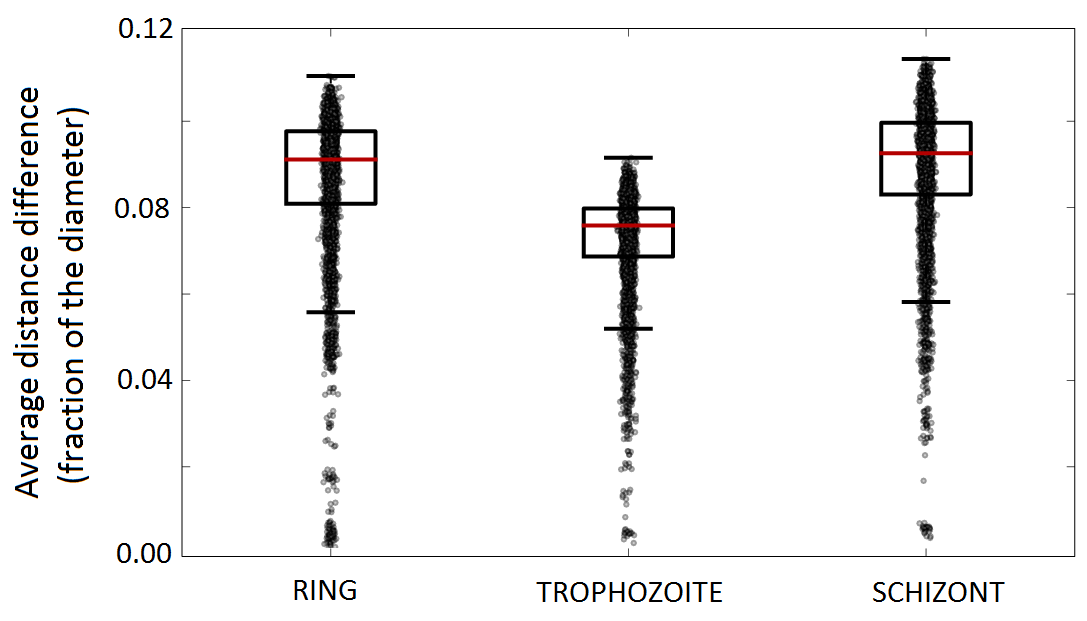
\includegraphics[width=0.8\textwidth]{suppFigs/stabilityOf3Dinference/compareStructurePairs.png}
   \end{center}
\caption{{\bf Similarity between 3D models inferred from 100 different initializations.}}
{We computed the average distance differences (Methods) for each pair of structures
(i.e., ${100 \choose 2}$) that are inferred from different initializations and
summarized these difference using a box plot for each stage. Each box extends from the
lower to upper quartile values with a red line at the median. These results show that
the 3D distance between a pair of loci varies, on the average, less than $10\%$ of the
nuclear diameter from one structure to another.
}
\label{suppfig:compareStructurePairs}
\end{figure}
\clearpage

% New fig
FIXME
\begin{figure}
  \begin{center}
  %\subfloat[Ring]{\includegraphics[width=0.85\textwidth]{suppFigs/3Dclustering/RINGS.pdf}} \hspace{0.15\textwidth}
  %\subfloat[Trophozoite]{\includegraphics[width=0.85\textwidth]{suppFigs/3Dclustering/TROPHOZOITES.pdf}}\hspace{0.15\textwidth}
  %\subfloat[Schizont]{\includegraphics[width=0.85\textwidth]{suppFigs/3Dclustering/SCHIZONTS.pdf}}
   \end{center}
\caption{{\bf Clustering of the 100 structures using pairwise RMSD values.}}
{ To assess whether the 100 structures generated from different random initializations fall into 
discrete clusters we performed hierarchical clustering on the pairwise RMSD matrix of each 
stage. We computed and plotted the Calinski-Harabasz (CH) 
index \cite{calinski:dendrite} for each clustering while varying the number of clusters from 2 to 50. 
None of the stages exhibited a clear peak of the CH index, suggesting that the set of structures do not fall into discrete clusters.
}
\label{suppfig:CHindices}
\end{figure}
\clearpage


\begin{figure}
  \begin{center}
  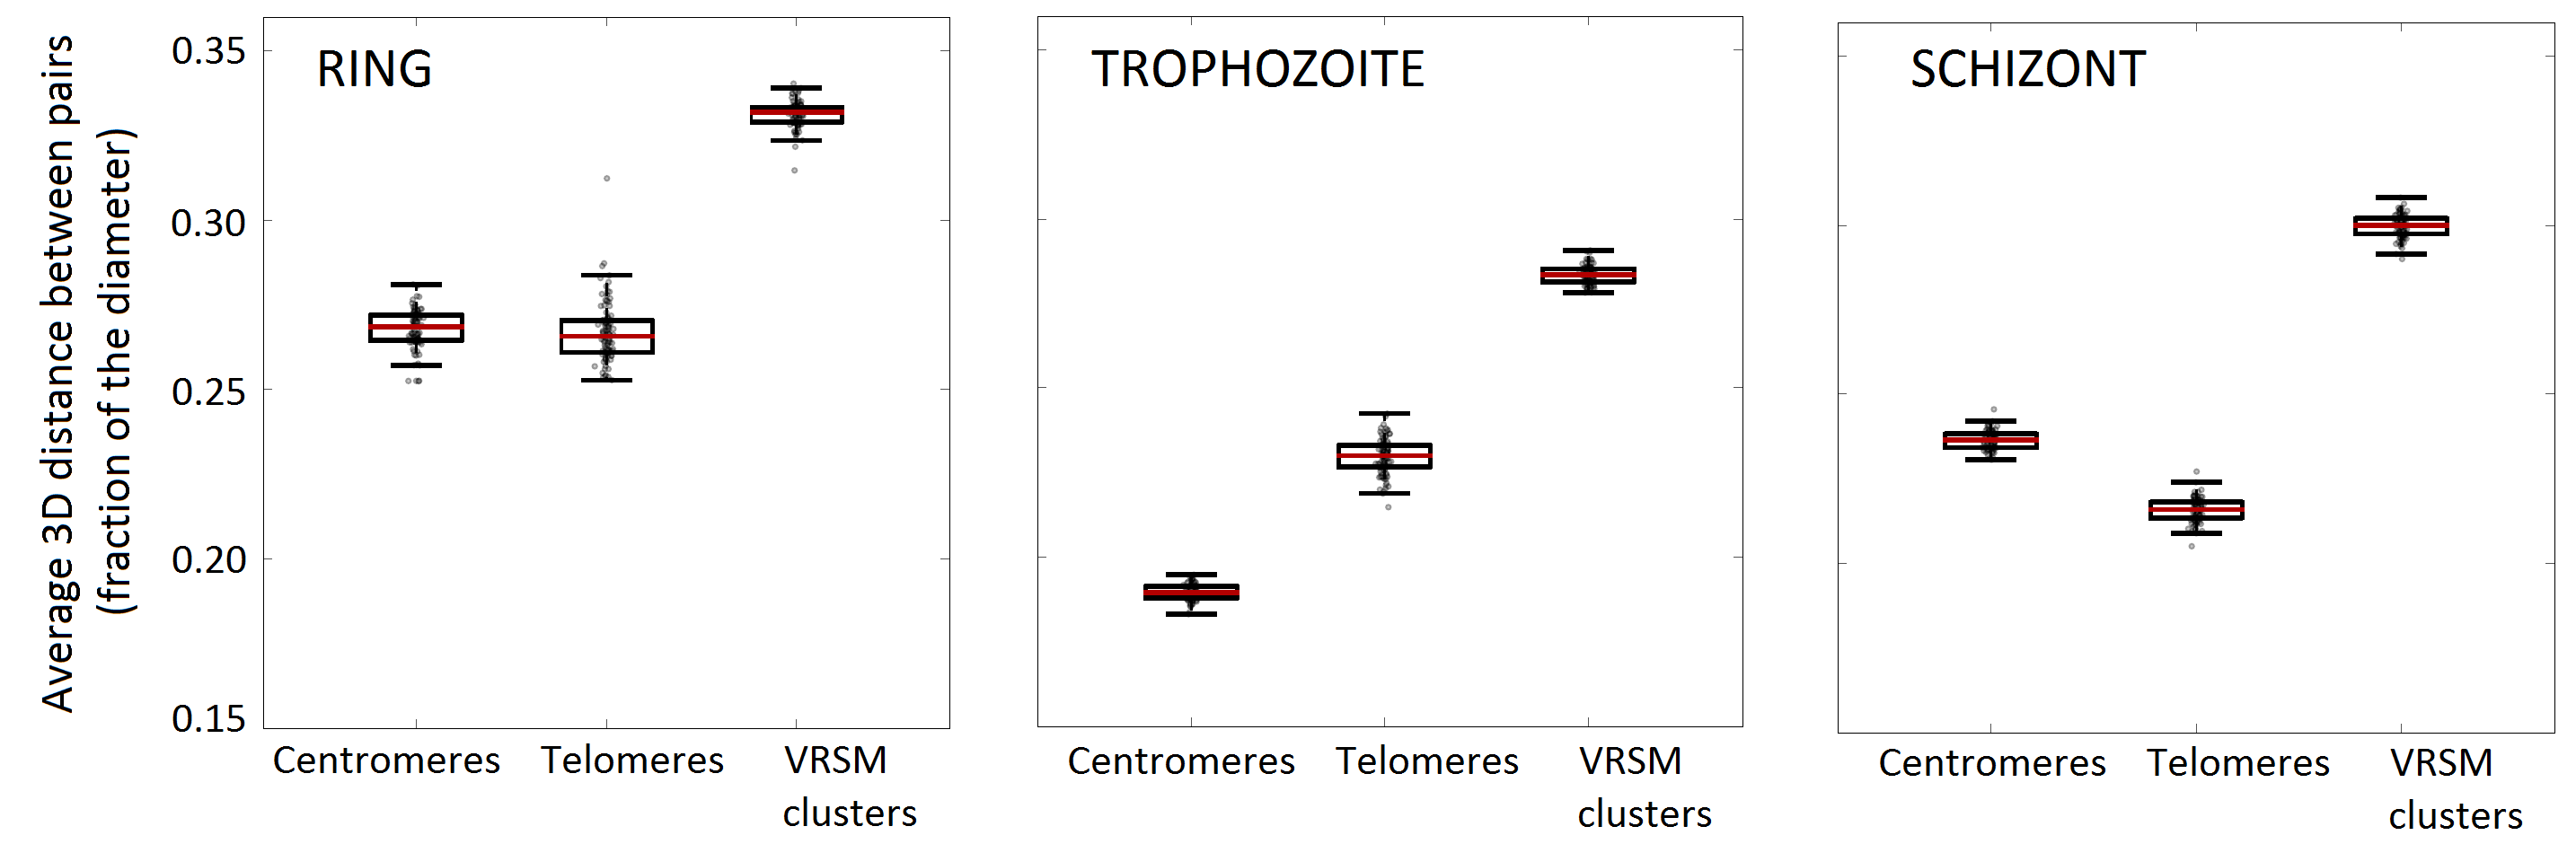
\includegraphics[width=1\textwidth]{suppFigs/stabilityOf3Dinference/allStages-clustering.png}
  \end{center}
\caption{{\bf Conservation of centromere, telomere and VRSM gene colocalizations across 100 different initializations. }}
{ We computed the average 3D distance between pairs of centromeres (${14 \choose 2}$ pairs),
telomeres (${28 \choose 2}$ pairs) and VRSM clusters (8 internal, 28 subtelomeric clusters and a total of ${36 \choose 2}$ pairs)
for each of the 100 structures inferred from different initializations and summarized
these average distances using a box plot for each stage. Each box extends from the
lower to upper quartile values with a red line at the median.  These results suggest that
the major organizational hallmarks concerning colocalization of centromere, telomere and
VRSM gene regions are common to all structures gathered from different initializations.}
\label{suppfig:clusteringIn100Structures}
\end{figure}
\clearpage




\begin{figure}
  \begin{center}
  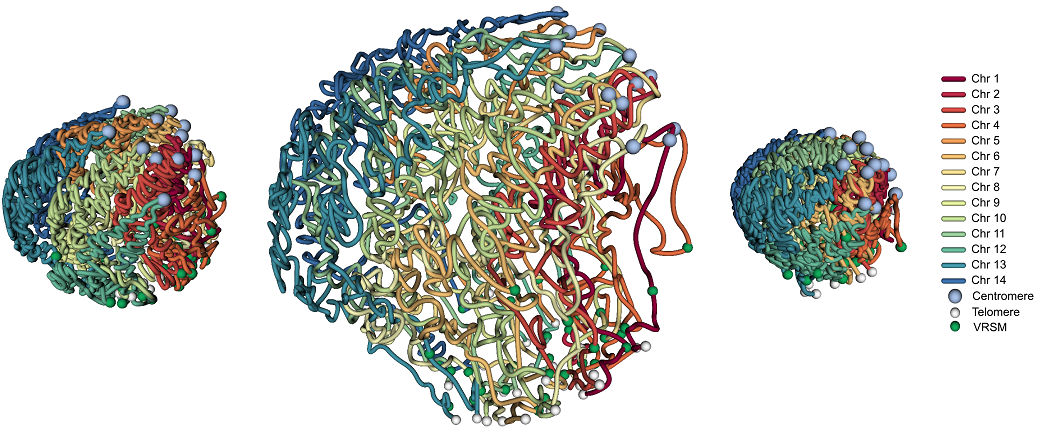
\includegraphics[width=1\textwidth]{suppFigs/3Dall/all3D-centromeres-angle-lowRes.png}
   \end{center}
\caption{{\bf 3D structures of all three stages (centromere clustering).}}
{This figure is identical to Main Figure 2a except the view is rotated to visualize the centromere
clustering for each stage. Centromeres and telomeres are indicated with light blue and white spheres,
respectively. Midpoints of VRSM gene clusters are shown with green spheres.}
\label{suppfig:3Dcentromeres}
\end{figure}
\clearpage


\begin{figure}
  \begin{center}
  \subfloat[Before clustering (Ring)]{\includegraphics[width=0.325\textwidth]{suppFigs/clusteringComparmentDists/RINGS.pdf}} \hspace{0.04\textwidth}
  \subfloat[Hierarchical clustering (Ring)]{\includegraphics[width=0.43\textwidth]{suppFigs/clusteringComparmentDists/RINGS-hierCluster-dists.pdf}} \hspace{0.1\textwidth}
  \subfloat[Before clustering (Trophozoite)]{\includegraphics[width=0.325\textwidth]{suppFigs/clusteringComparmentDists/TROPHOZOITES-XL.pdf}} \hspace{0.04\textwidth}
  \subfloat[Hierarchical clustering (Trophozoite)]{\includegraphics[width=0.43\textwidth]{suppFigs/clusteringComparmentDists/TROPHOZOITES-XL-hierCluster-dists.pdf}} \hspace{0.1\textwidth}
  \subfloat[Before clustering (Schizont)]{\includegraphics[width=0.325\textwidth]{suppFigs/clusteringComparmentDists/SCHIZONTS.pdf}} \hspace{0.04\textwidth}
  \subfloat[Hierarchical clustering (Schizont)]{\includegraphics[width=0.43\textwidth]{suppFigs/clusteringComparmentDists/SCHIZONTS-hierCluster-dists.pdf}}
  \end{center}
\caption{{\bf Hierarchical clustering of compartment distance matrices. }}
{Pairwise compartment distance matrices ($42\times42$, three compartments on each chromosome) that are identified
    by eigenvalue decomposition (Methods) for (a) ring, (c) trophozoite and (e) schizont stages. Distances are
    averaged over all pairs of loci between the two compartments and normalized using nuclear diameter to result
    in a fraction between 0 and 1. In the figure, the actual length of each compartment and each chromosome are preserved.
    Each compartment is colored separately, with dashed lines segregating adjacent chromosomes.
    Hierarchical clustering of pairwise compartment distance matrices for (b) ring, (d) trophozoite and
    (f) schizont stages. Clustering was performed using the average linkage score.
    Each compartment is represented by a fixed length, and L, M, R denote left, mid, right
    compartments, respectively. For all panels the color bars extend from 0 to 0.5
    (i.e., distance equals nuclear radius).
}
\label{suppfig:compDists}
\end{figure}
\clearpage

\begin{figure}
  \begin{center}
  \subfloat[]{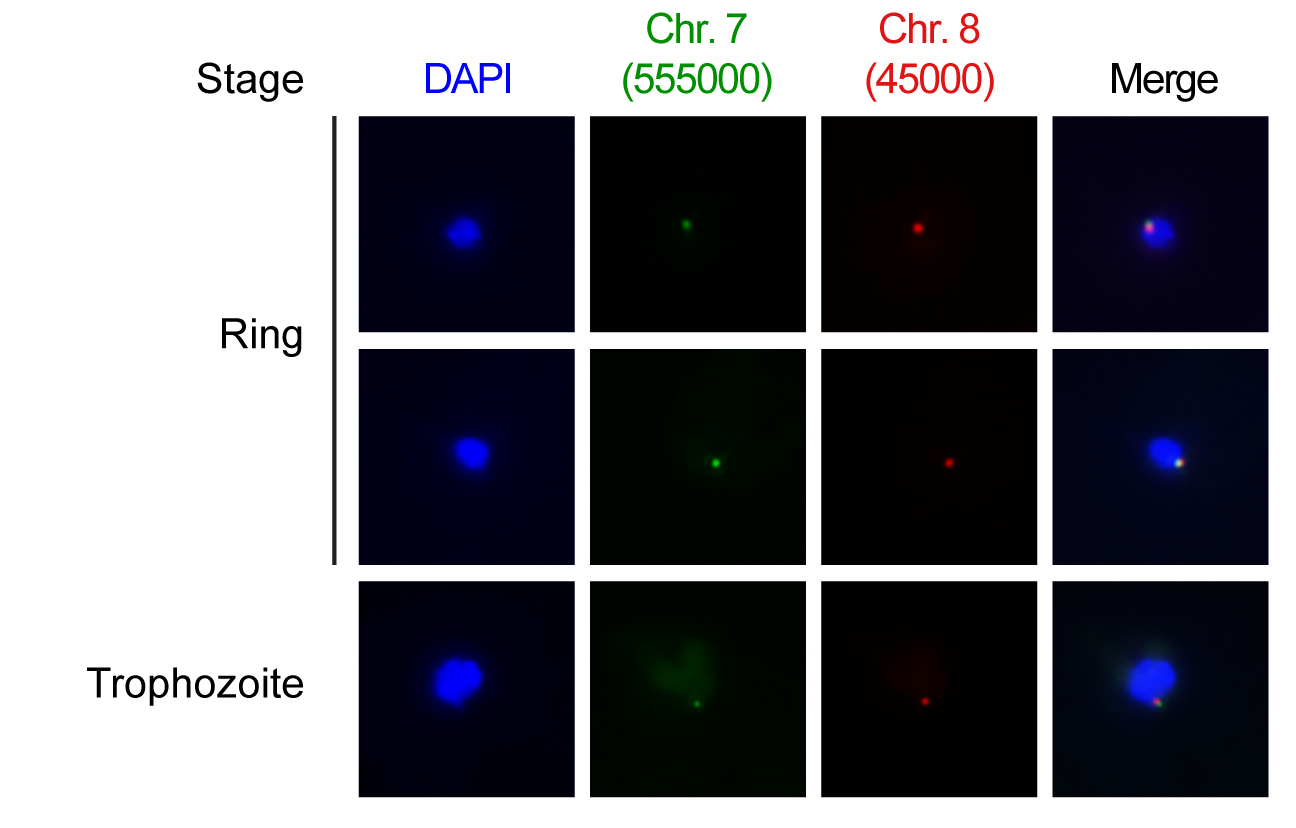
\includegraphics[width=0.69\textwidth]{suppFigs/FISH/varPair.png}} \\
  \subfloat[]{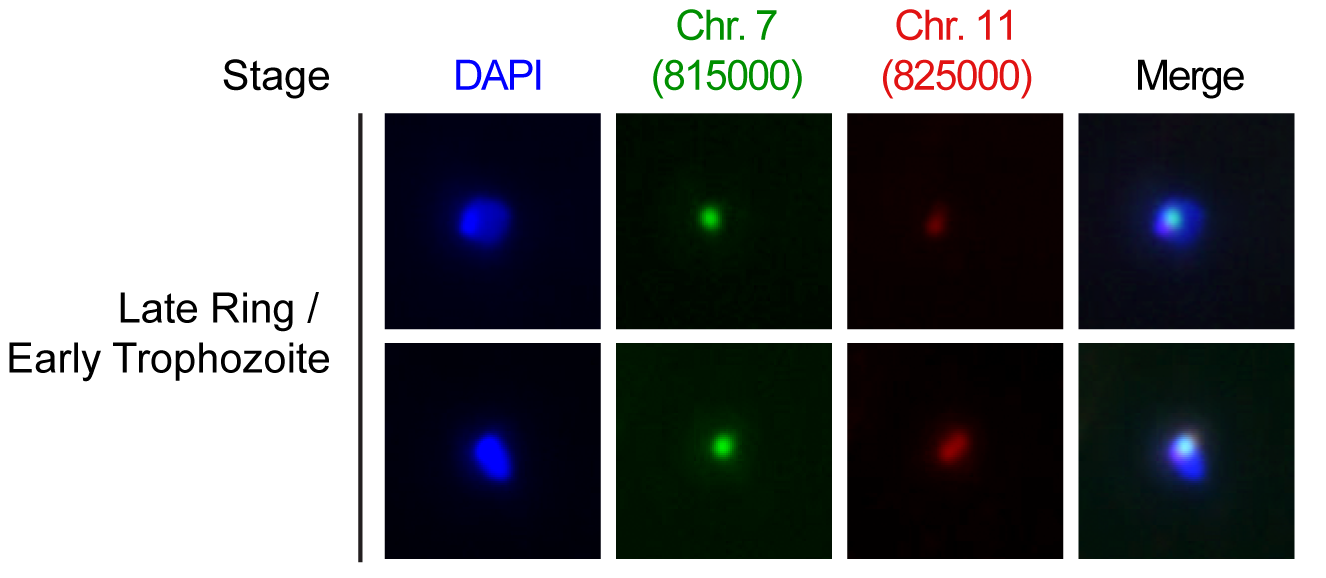
\includegraphics[width=0.69\textwidth]{suppFigs/FISH/nonvarPair.png}} \\
  \hspace{0.015\textwidth}
  \subfloat[]{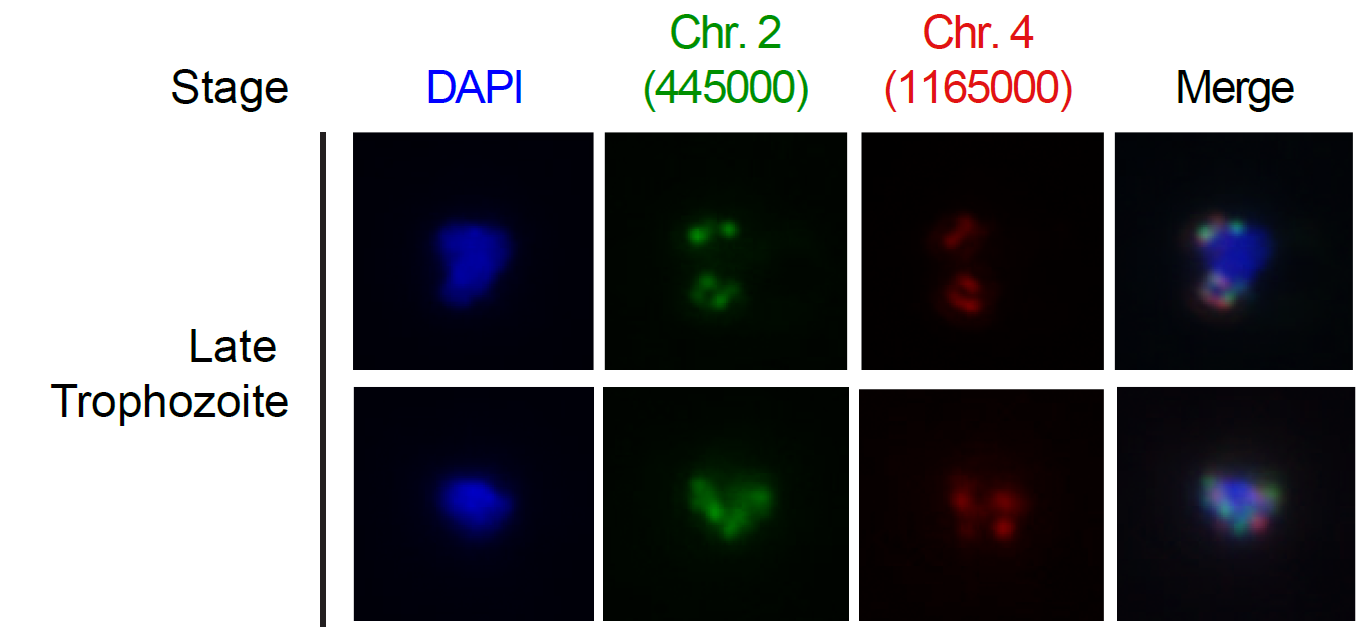
\includegraphics[width=0.65\textwidth]{suppFigs/FISH/controlPair.png}}\\
  \end{center}
\caption{{\bf Validation of 3D models with DNA FISH.}}
{ Additional FISH images for (a) a pair of interchromosomal loci with VRSM
  genes (chr7:550,000-560,000 containing internal VRSM genes and
  chr8:40,000-50,000 containing subtelomeric VRSM genes)
  (b) a pair of interchromosomal loci that harbor no VRSM genes
  (chr7:810,000-820,000 and chr11:820,000-830,000).
  (c) FISH images showing lack of colocalization as a negative
  control for a pair of interchromosomal loci that harbor no VRSM genes
  and have no contacts in trophozoite stage (chr2:440,000-450,000 and chr4:1,160,000-1,170,000).
}
\label{suppfig:fish}
\end{figure}
\clearpage

\begin{figure}
  \begin{center}
%  \subfloat[Our data - Ring]{\includegraphics[width=0.32\textwidth]{suppFigs/Newbold-virtual4Cs/RINGS/chr7-rDNA/chr5.pdf}} \hspace{0.05\textwidth}
%  \subfloat[Our data - Trophozoite]{\includegraphics[width=0.32\textwidth]{suppFigs/Newbold-virtual4Cs/TROPHOZOITES-XL/chr7-rDNA/chr5.pdf}} \vspace{-0.01\textwidth}
%  \subfloat[Our data - Schizont]{\includegraphics[width=0.32\textwidth]{suppFigs/Newbold-virtual4Cs/SCHIZONTS/chr7-rDNA/chr5.pdf}} \hspace{0.05\textwidth}
%  \subfloat[Our data - Trophozoite control]{\includegraphics[width=0.32\textwidth]{suppFigs/Newbold-virtual4Cs/TROPHOZOITES-NL/chr7-rDNA/chr5.pdf}}
%  \vspace{-0.01\textwidth}
%	
  \subfloat[Lemieux et al. data - DCJ
  On]{\includegraphics[width=0.32\textwidth]{suppFigs/Newbold-virtual4Cs/\detokenize{DCJ_On-HiC-MboI}/chr7-rDNA/chr5.pdf}} \hspace{0.05\textwidth}
  \subfloat[Lemieux et al. data - DCJ
  Off]{\includegraphics[width=0.32\textwidth]{suppFigs/Newbold-virtual4Cs/\detokenize{DCJ_Off-HiC-MboI}/chr7-rDNA/chr5.pdf}} \vspace{-0.01\textwidth}
  \subfloat[Lemieux et al. data - B15C2]{\includegraphics[width=0.32\textwidth]{suppFigs/Newbold-virtual4Cs/B15C2-HiC-MboI/chr7-rDNA/chr5.pdf}}
  \hspace{0.05\textwidth}
  \subfloat[Lemieux et al. data - NF54 control]{\includegraphics[width=0.32\textwidth]{suppFigs/Newbold-virtual4Cs/NF54-Control-MboI/chr7-rDNA/chr5.pdf}}
  \end{center}
\caption{{\bf Clustering of highly transcribed rDNA units in Lemieux et al. data.}}
{Hi-C libraries generated with MboI restriction enzyme
    from Lemieux et al. \cite{lemieux:genome-wide}  were mapped
    to the \emph{P. falciparum} genome and further processed using the
    pipeline we processed our data with to generate and normalize contact maps at 25 kb resolution.
    The normalized contact maps were used for virtual 4C plots using as a bait
    the A-type rDNA unit on chromosome 7. As suggested in Lemieux et al.,
    contact counts from 50 kb up- and downstream of the 25 kb bin containing
    rDNA unit were used, and the rDNA-containing window itself was removed
    from the analysis. For each window $w$ on chromosome 5, the contact
    enrichment was calculated by dividing the contact count between
    the bait and $w$ to the average interchromosomal contact count for
    the bait locus.
}
\label{suppfig:rDNAunitsOn3D}
\end{figure}
\clearpage



\begin{figure}
\begin{center}
\subfloat{
    \begin{tabular}{ccc}
      \includegraphics[width=0.33\textwidth]{suppFigs/intraVSinter/per10kb-B15C2-HiC-MboI.pdf}  & \hspace{0.1\textwidth} & \includegraphics[width=0.33\textwidth]{suppFigs/intraVSinter/equalOcc-B15C2-HiC-MboI.pdf} \\
      (a) Lemieux et al. data - B15C2 & \hspace{0.1\textwidth} & (b) Lemieux et al. data - B15C2 \\
      & & \\
        \includegraphics[width=0.33\textwidth]{suppFigs/intraVSinter/equalOcc-RINGS.pdf}	& \hspace{0.1\textwidth} & \includegraphics[width=0.33\textwidth]{suppFigs/intraVSinter/equalOcc-TROPHOZOITES-XL.pdf} \\
		(c) Our data - Ring & \hspace{0.1\textwidth} & (d) Our data  - Trophozoite\\
      & & \\
        \multicolumn{3}{c}{\includegraphics[width=0.33\textwidth]{suppFigs/intraVSinter/equalOcc-SCHIZONTS.pdf}} \\
		\multicolumn{3}{c}{(e) Our data - Schizont}
    \end{tabular}
}
\end{center}
\caption{{\bf Comparison of inter and intrachromosomal contact prevalence. }}
{ The relationship between contact count and genomic distance is estimated
    using bins with equal genomic distances (e.g., 10 kb, 20 kb) in Lemieux
    et al. \cite{lemieux:genome-wide}. Due to the diminishing number of possible
    locus pairs with increasing genomic distance (e.g., only one locus pair for
    the bin with the largest genomic distance) this estimation leads to many
    high variance bins for large genomic distances. This issue can be addressed
    by using variable-width bins that contain equal numbers of
    contacts (see Methods). Plotted are the $\log$ (base $e$) of mean
    contact count per bin when using (a) equal distance binning, (b)
    equal occupancy binning for B15C2 library of Lemieux et
    al. \cite{lemieux:genome-wide} and (c-e) equal occupancy binning for
    ring, trophozoite and schizont stage data from this work. Dashed vertical
    red lines denote the range used to compute the log-linear fit.
}
\label{suppfig:intraVSinter}
\end{figure}
\clearpage

\begin{figure}
  \begin{center}
  \includegraphics[width=0.8\textwidth]{suppFigs/chrTerritory/diam2point5.pdf}
   \end{center}
\caption{{\bf Changes in chromosome territories during the erythrocytic cycle.}}
{ The extent to which a chromosome intermingles with other chromosomes is
    characterized by the percentage of nuclear volume that is jointly occupied
    by the chromosome of interest and at least one other chromosome,
    relative to the entire volume occupied by the chromosome.
    To compute the percentages on the y-axis, the nuclear volume was sampled using
    1,000,000 randomly generated small spheres with radius 5\% of the actual nuclear
    radius. For each chromosome $i$, two numbers were calculated: the number of spheres that contain a locus
    from chromosome $i$ ($n_i$) and the number of such spheres that
    contain no locus from another chromosome ($e_i$). The percent intermingled (y-axis)
    for chromosome $i$ is computed as $100\times \frac{n_i-e_i}{n_i}$.
    Because the exact percentages are highly dependent on the selection of the random
    sphere size, the procedure was repeated using spheres with
    radii 2\%, 10\% and 20\% of the nuclear volume.  For each setting,
    the trophozoite stage exhibited the highest amount of intermingling,
    whereas the schizont stage showed the lowest. Also, the
    larger chromosomes (i.e., chromosomes with higher numbers)
    consistently showed lower intermingling compared to smaller
    chromosomes at each stage and for each threshold.}
\label{suppfig:territory}
\end{figure}
\clearpage


\begin{figure}
  \begin{center}
%  \subfloat[]{\includegraphics[width=0.55\textwidth]{suppFigs/clusteringComparmentDists/RINGS.png}}
  \subfloat[From ring to trophozoite]{\includegraphics[width=0.6\textwidth]{suppFigs/clusteringComparmentDists/RINGS-minus-TROPHOZOITES-XL.pdf}}
  \hspace{0.03\textwidth}
%  \subfloat[]{\includegraphics[width=0.55\textwidth]{suppFigs/clusteringComparmentDists/TROPHOZOITES-XL.png}}
  \subfloat[From trophozoite to schizont]{\includegraphics[width=0.6\textwidth]{suppFigs/clusteringComparmentDists/TROPHOZOITES-XL-minus-SCHIZONTS.pdf}}
%  \subfloat[]{\includegraphics[width=0.55\textwidth]{suppFigs/clusteringComparmentDists/SCHIZONTS.png}}
%  \subfloat[]{\includegraphics[width=0.55\textwidth]{suppFigs/clusteringComparmentDists/SCHIZONTS-hierCluster-dists.png}}
  \end{center}
\caption{{\bf Movement of chromosome compartments with respect to each other.}}
{ Each compartment movement matrix is generated by subtracting the pairwise compartment
    distance matrix (Supplementary Fig. \ref{suppfig:compDists}) of one stage from the
    matrix of the preceding stage. Plotted are the movements (a) from ring to trophozoite
    (i.e., trophozoite minus ring), (b) from trophozoite to schizont (i.e.,  schizont minus
    trophozoite). Red color indicates that a pair of compartments are closer in the later
    stage compared to the earlier, and blue color indicates vice versa.
}
\label{suppfig:compMovement}
\end{figure}
\clearpage


\begin{figure}
  \begin{center}
  \subfloat[]{\includegraphics[width=0.7\textwidth]{suppFigs/VE/correlation-per-num-experiments.png}}
  \hspace{0.03\textwidth}
  \subfloat[]{
  \begin{tabular}{llcccc}
    \hline
    \emph{Contact map 1} & \emph{Contact map 2} & \emph{Row-based corr.} & \emph{Normalized row-based corr.}   \\
    \hline
    \multirow{2}{*}{Yeast \textit{(Hi-C)\cite{duan:three}}} &Yeast \textit{(VE)} & 0.915 & 0.573 \\
    & Yeast \textit{(expected)} & 0.922 & 0.115 \\\hline
    \multirow{2}{*}{Ring \textit{(Hi-C)}} &Ring \textit{(VE)} & 0.843 & 0.340 \\
    & Ring \textit{(expected)} & 0.928 & 0.072 \\\hline
    \multirow{2}{*}{Trophozoite \textit{(Hi-C)}} &Trophozoite \textit{(VE)} & 0.848 & 0.392 \\
    & Trophozoite \textit{(expected)} & 0.908 & 0.063 \\\hline
    \multirow{2}{*}{Schizont \textit{(Hi-C)}} &Schizont \textit{(VE)} & 0.864 & 0.487 \\
    & Schizont \textit{(expected)} & 0.923 & 0.081 \\
    \hline
    \end{tabular}}
  \end{center}
\caption{{\bf Volume exclusion modeling and correlation calculation.}}
{ (a) Row-based Pearson correlation between the observed Hi-C contact map
    and the average contact map from volume exclusion modeling as a function
    of the number of simulated structures.
    (b) Row-based Pearson correlation and normalized row-based Pearson
    correlation between the two contact maps listed in each row for
    various Hi-C libraries. \emph{VE} refers to
    contact maps obtained from 5000 structures generated by volume exclusion
    and \emph{expected} refers to matrices with expected contact counts
    generated from observed \emph{Hi-C} matrices as described in Methods.
    }
\label{suppfig:VEconvergence}
\end{figure}
\clearpage


\begin{figure}
\begin{center}
\subfloat[]{\includegraphics[width=3in]{suppFigs/TADs/TAD-descriptive.png}}
\hspace{0.03\textwidth}
\subfloat[]{\begin{tabular}{lccccc}
\hline
%\multirow{2}{*} {\emph{Internal VRSM}} & \multirow{2}{*}{\emph{Stage}} & \multirow{2}{*}{Mean($\frac{t_2-t_1}{t_2+t_1}$)} & \multirow{2}{*}{Mean($\frac{t_2-t_3}{t_2+t_3}$)} & \multirow{2}{*}{Mean($\frac{r_5-r_4}{r_5+r_4}$)} & \multirow{2}{*}{Mean($\frac{r_6-r_7}{r_6+r_7}$)} \\
%& & & & &\\\hline
%% OR
\emph{Internal VRSM} & \emph{Stage} & $t_2$ vs. $t_1$ & $t_2$
vs. $t_3$ & $r_5$ vs. $r_4$ & $r_6$ vs. $r_7$ \\ \hline
\multirow{3}{*} {chr4(1)}	&	R	&	\cellcolor[gray]{0.8}0  &	0.7  &  \cellcolor[gray]{0.8}0  &  -0.09 \\
	&	T	&	0.06	&	0.2  &  -0.11  &  -0.25 \\
	&	S	&	0.1  &	0.16  &  \cellcolor[gray]{0.8}0.13  &  -0.14 \\\hline
\multirow{3}{*} {chr4(2)}	&	R	&	0.13	&	0.12  &  -0.38  &  -0.27 \\
	&	T	&	0.15	&	0.15  &  -0.42  &  -0.33 \\
	&	S	&	0.14	&	0.13  &  -0.37  &  -0.3 \\\hline
\multirow{3}{*} {chr4(3)}	&	R	&	0.03	&	0.08  &  -0.37  &  -0.34 \\
	&	T	&	0.03	&	0.06  &  -0.55  &  -0.41 \\
	&	S	&	0.03	&	0.01  &  -0.48  &  -0.42 \\\hline
\multirow{3}{*} {chr6(1)}	&	R	&	0.12	&	0.1  &  \cellcolor[gray]{0.8}0.02  &  -0.06 \\
	&	T	&	0.19	&	0.2  &  -0.09  &  -0.16 \\
	&	S	&	0.16	&	0.18  &  -0.08  &  -0.14 \\\hline
\multirow{3}{*} {chr7(1)}	&	R	&	0.11	&	0.2  &  -0.19  &  -0.18 \\
	&	T	&	0.19	&	0.28  &  -0.36  &  -0.3 \\
	&	S	&	0.08	&	0.19  &  -0.27  &  -0.27 \\\hline
\multirow{3}{*} {chr8(1)}	&	R	&	0.15	&	0.08  &  -0.05  &  -0.09 \\
	&	T	&	0.17	&	0.09  &  -0.17  &  -0.13 \\
	&	S	&	0.14	&	0.09  &  -0.11  &  -0.11 \\\hline
\multirow{3}{*} {chr12(1)}	&	R	&	0.07	&	0.05  &  -0.02  &  -0.01 \\
	&	T	&	0.05	&	0.14  &  -0.04  &  -0.02 \\
	&	S	&	0.09	&	0.12  &  -0.07  &  -0.08 \\\hline
\multirow{3}{*} {chr12(2)}	&	R	&	0.09	&	0.09  &  -0.09  &  -0.11 \\
	&	T	&	0.17	&	0.1  &  -0.27  &  -0.24 \\
	&	S	&	0.09	&	0.07  &  -0.19  &  -0.23 \\\hline
\end{tabular}
}
\end{center}
\caption{{\bf Quantification of domain-like behavior of VRSM gene
    clusters.}} {(a) Each internal VRSM gene cluster is characterized
  by a set of strong intra-cluster contacts ($t_2$) and two sets of
  contacts with adjacent regions ($r_5$ and $r_6$) that are weak. For
  comparison, we also consider flanking, non-VSRM regions of the same
  size as the original VRSM cluster, including their ``intra-cluster''
  contacts ($t_1$ and $t_3$) which should be similar to $t_2$ for
  a contact map without domain-like structures around VRSM clusters
  and contacts with adjacent regions ($r_4$ and $r_7$) which are
  comparable to ($r_5$ and $r_6$). As seen in this example,
  a domain-like structure for a VRSM cluster leads to stronger
  contacts (+ sign) within $t_2$ compared to both $t_1$ and $t_3$, and weaker
  contacts (- sign) within $r_4$ and $r_7$ compared to $r_5$ and $r_6$.
  (b) The table reports, for each internal
  VRSM gene cluster and each stage, the average normalized difference between
  the intra-cluster contacts within the cluster compared to its
  two flanking control regions, and similarly for the contacts
  with adjacent regions.  The metric we use for comparing two contact
  sub-matrices $X$, $Y$ of
  dimension $N \times M$ is $\frac{1}{NM} \sum_{i=1}^N \sum_{j=1}^M
  \frac{x_{ij} - y_{ij}}{\frac{1}{2}(x_{ij}+y_{ij})}$ where $x_{ij}$ and
  $y_{ij}$ are the $ij$th entries of $X$ and $Y$, respectively.
  Values that have signs inconsistent with the expected pattern
  (i.e., +, +, -, -) are indicated with a grey background. Every internal
  VRSM cluster exhibits the expected sign pattern in at least one stage.
  }
\label{suppfig:TADs}
\end{figure}
\clearpage

\begin{figure}
  \begin{center}
  \subfloat[All genes]{\includegraphics[width=0.45\textwidth]{suppFigs/expVSdists/all-corr-contactCounts.pdf}}
  \hspace{0.05\textwidth}
  \subfloat[Excluding VRSM genes]{\includegraphics[width=0.45\textwidth]{suppFigs/expVSdists/all-corr-contactCounts-withoutVRSM.pdf}}
  \hspace{0.05\textwidth}
  \subfloat[All genes]{\includegraphics[width=0.45\textwidth]{suppFigs/expVSdists/all-100-3Ddists.pdf}}
  \hspace{0.05\textwidth}
  \subfloat[Excluding VRSM genes]{\includegraphics[width=0.45\textwidth]{suppFigs/expVSdists/all-100-3Ddists-withoutVRSM.pdf}}
%  \hspace{0.05\textwidth}
%  \subfloat[All genes]{\includegraphics[width=0.45\textwidth]{suppFigs/expVSdists/all-corr.pdf}}
%  \hspace{0.05\textwidth}
%  \subfloat[Excluding VRSM genes]{\includegraphics[width=0.45\textwidth]{suppFigs/expVSdists/all-corr-withoutVRSM.pdf}}
   \end{center}
\caption{{\bf Revisiting the relationship between 3D architecture and gene expression by excluding VRSM genes. }}
{   (a) is identical to Main Figure 6a and (b) is generated identical to (a) except all gene pairs
    involving at least one VRSM gene are omitted from the analysis. Re-evaluation of our
    hypothesis that interchromosomal gene pairs that have contact counts within the top 20\%
    for each stage have more highly correlated expression profiles than the remaining gene pairs
    still yielded significant p-values for each stage [Wilcoxon rank-sum test, p-values 1.07e-70 (ring),
    0 (trophozoite), and 1.68e-302 (schizont)].
    (c) is identical to Main Figure 6b and (d) is generated identical to (c) except all gene pairs
    involving at least one VRSM gene are omitted from the analysis. Re-evaluation of our
    hypothesis that interchromosomal gene pairs closer than 20\% of the nuclear diameter have more
    highly correlated expression profiles than other genes still yielded
    significant p-values for each stage [Wilcoxon rank-sum test, p-values 3.27e-48 (ring),
    1.32e-157 (trophozoite), and 2.16e-5 (schizont)].
}
\label{suppfig:expVSdistWithoutVRSM}
\end{figure}
\clearpage

\begin{figure}
  \begin{center}
  \subfloat[All genes]{\includegraphics[width=0.45\textwidth]{suppFigs/expVSdists/telomeres-100-corr.pdf}}
  \hspace{0.05\textwidth}
  \subfloat[Excluding VRSM genes]{\includegraphics[width=0.45\textwidth]{suppFigs/expVSdists/telomeres-100-corr-withoutVRSM.pdf}}
  \hspace{0.05\textwidth}
  \subfloat[All genes]{\includegraphics[width=0.45\textwidth]{suppFigs/expVSdists/centromeres-100-corr.pdf}}
  \hspace{0.05\textwidth}
  \subfloat[All genes]{\includegraphics[width=0.45\textwidth]{suppFigs/expVSdists/center-100-corr.pdf}}
   \end{center}
\caption{{\bf The relationship between distance to the telomeres, nuclear center and centromeres versus the gene expression.}}
{   (a) is identical to Main Figure 6c and (b) is generated identical to (a) except
    all VRSM genes are omitted from the analysis.
    Re-evaluation of our hypothesis that genes which lie within a distance of
    20\% of the nuclear diameter to the centroid of the telomeres exhibit lower expression
    levels yielded a significant p-value for trophozoite stage but not for ring and
    schizont stages at a significance threshold of $0.01$ [Wilcoxon rank-sum test,
    p-values 0.21 (ring), 1.5e-3 (trophozoite), and 0.035 (schizont)].
    (c) and (d) are generated identical to (a) expect the distance of genes are measured to
    (c) the centroid of the centromeres and (d) the nuclear center.
    For each figure, genes are first sorted in increasing order according to their distances
    to the landmark of interest and then binned into 20 equal width quantiles
    ($5$th, $10$th, ..., $100$th). For each bin, the average distance to the landmark (x-axis)
    and the average log expression value~\citep{bunnik:polysome} together with its standard
    error (y-axis) are computed and plotted.
}
\label{suppfig:distToCenter}
\end{figure}
\clearpage


\begin{figure}
\begin{center}
\subfloat{
    \begin{tabular}{ccc}
      \includegraphics[width=0.28\textwidth]{suppFigs/kCCA/RINGS-kcca-genes-1.png} & \hspace{0.1\textwidth} & \includegraphics[width=0.28\textwidth]{suppFigs/kCCA/RINGS-kcca-genes-2.png} \\
      (a) First component (Ring) & \hspace{0.1\textwidth} & (b) Second component (Ring) \\
     % & & \\
        \includegraphics[width=0.28\textwidth, angle=-165]{suppFigs/kCCA/TROPH-kcca-genes-1.png} & \hspace{0.1\textwidth} & \includegraphics[width=0.28\textwidth, angle=-165]{suppFigs/kCCA/TROPH-kcca-genes-2.png} \\
      (c) First component (Trophozoite) & \hspace{0.1\textwidth} & (d) Second component (Trophozoite) \\
      %& & \\
        \includegraphics[width=0.28\textwidth, angle=-25]{suppFigs/kCCA/SCHIZONTS-kcca-genes-1.png} & \hspace{0.1\textwidth} & \includegraphics[width=0.28\textwidth, angle=-25]{suppFigs/kCCA/SCHIZONTS-kcca-genes-2.png} \\
      (e) First component (Schizont) & \hspace{0.1\textwidth} & (f) Second component (Schizont) \\
      %& & \\
      \multicolumn{3}{c}{\includegraphics[width=0.3\textwidth]{suppFigs/kCCA/legend.png}} \\
    \end{tabular}
}
\end{center}
\caption{{\bf kCCA expression profiles component score.}}  { Each
  panel shows the projection of the gene expression profile onto one
  of the two extracted kCCA profiles for a specified erythrocytic
  stage, with the score of the projection encoded on the color
  scale. For the first kCCA component, the projections consistently
  exhibit a striking gradient from the telomeric region across
  the nucleus, while for the second component, which is less coherent
  with the 3D structure, the projection gradient extends from the
  centromeres across the nucleus.  }
\label{suppfig:kCCAsecond}
\end{figure}
\clearpage


% ================== FIGURES THAT MAY NOT END UP BEING REFERRED TO ==================



% ================================================================================
% SUPPLEMENTARY METHODS
\section*{Supplementary Notes}
%\addcontentsline{toc}{section}{Supplementary Results}
\phantomsection

\addcontentsline{toc}{subsection}{{\bf 1} \indent {\bf Tethered conformation capture procedure protocol}}
\subsection*{Supplementary Note 1: Tethered conformation capture procedure}
\label{supp:ourHiC}
\paragraph{Day 1}
 Parasite pellets were thawed on
ice in 550 $\mu$l Hi-C lysis buffer (25 mM Tris-HCl at pH 8.0, 10 mM NaCl,
2 mM AEBSF, Roche Complete Mini EDTA-free protease inhibitor cocktail
[Roche, Basel, Switzerland], 0.25\% Igepal CA-630) per 140
mg. Parasite membranes were disrupted by passing the lysate through a
26.5 gauge needle 15 times using a syringe. Samples were spun at 2,500
$\times$ g for 5 min at room temperature (RT). Pellets were washed twice with
1 ml ice-cold wash buffer (50 mM Tris-HCl at pH 8.0, 50 mM NaCl, 1 mM
EDTA) and resuspended in the same buffer to a final volume of 250
$\mu$l. Samples were mixed with 95 $\mu$l 2\% SDS to a final concentration of
0.5\% and incubated at 55$^\circ$C for 15 min. Suspensions were cooled down
to RT before they were mixed with 105 $\mu$l 25 mM EZ-link
Iodoacetyl-PEG2-Biotin (IPB) (Thermo Fisher Scientific, Waltham, MA,
USA) to biotinylate proteins. After incubating for 1 h at RT while
rotating, the SDS was neutralized by adding 1.3 ml 1$\times$ NEBuffer 2 (New
England Biolabs [NEB], Ipswich, MA, USA). Samples were mixed with 225
$\mu$l 10\% Triton X-100 to a final concentration of 1\% and incubated for
10 min on ice, followed by 10 min at 37$^\circ$C. Five $\mu$l 1 M DTT, 100 $\mu$l 10$\times$
NEBuffer 2, 415 $\mu$l water and 35 $\mu$l MboI restriction enzyme (NEB) (25
units/$\mu$l) was added to digest the DNA overnight at 37$^\circ$C in a total
volume of 2,530 $\mu$l.

\paragraph{Day 2}
After digestion, samples were loaded into a Slide-A-Lyzer Dialysis
Cassette G2 (Thermo Fisher Scientific) and dialyzed for 4 h at RT
against 1 L of dialysis buffer (10 mM Tris-HCl at pH 8.0, 1 mM EDTA)
to eliminate excess IPB remaining from the biotinylation
step. Dialysis buffer was renewed after 3 h. Four hundred $\mu$l MyOne
Streptavidin T1 beads (Life Technologies, Carlsbad, CA, USA) were
washed 3 times with PBS + 0.01\% Tween-20 (PBST) and beads were
resuspended in 2 ml PBST. Dialyzed samples were divided into 5 equal
aliquots of 500 $\mu$l in 1.7 ml prelubricated microcentrifuge tubes
(Corning, Corning, NY, USA). Four hundred $\mu$l beads were added to each
tube and samples were incubated for 30 min at RT while rotating. To
prevent interference of unbound streptavidin on the beads with later
steps (adding biotinylated dCTP) 5 $\mu$l neutralized IPB was added to
each tube. IPB was neutralized by adding an equimolar amount of
2-mercaptoethanol. Samples were incubated for an additional 15 min at
RT while rotating. Not biotinylated chromatin and not cross-linked DNA
was removed by washing the magnetic T1 beads once with 600 $\mu$l PBST and
once with 600 $\mu$l wash buffer (10 mM Tris-HCl at pH 8.0, 50 mM NaCl,
0.4\% Triton X-100). Beads were resuspended in 100 $\mu$l of the same wash
buffer. MboI generated $5'$ overhangs were filled in by adding 63 $\mu$l
water, 1 $\mu$l 1 M MgCl, 10 $\mu$l 10$\times$ NEBuffer 2, 0.7 $\mu$l 10 mM dATP, 0.7 $\mu$l
10 mM dTTP, 0.7 $\mu$l 10 mM 2'-Deoxyguanosine-5'-O-(1-thiotriphosphate),
sodium salt, Sp-isomer (Axxora, San Diego, CA, USA), 15 $\mu$l 0.4 mM
Biotin-14-dCTP (Life Technologies), 4 $\mu$l 10\% Triton X-100 and 5 $\mu$l
5U/$\mu$l DNA Polymerase I, Large (Klenow) Fragment (NEB). Samples were
incubated for 40 min at RT while rotating. Reaction was stopped by
adding 5 $\mu$l 0.5 M EDTA to the suspension. After 2 min of incubation at
RT while rotating, beads were washed twice with 600 $\mu$l buffer (50 mM
Tris-HCl at pH 7.4, 0.4\% Triton X-100, 0.1 mM EDTA) and resuspended
in 500 $\mu$l of the same buffer. Each sample was transferred into a 15 ml
centrifuge tube. For blunt-end ligation under dilute conditions 500 $\mu$l
sample was mixed with 4 ml water, 250 $\mu$l 10$\times$ Ligase Buffer (NEB), 100
$\mu$l 1 M Tris-HCl at pH 7.4, 90 $\mu$l 20\% Triton X-100, 50 $\mu$l 100$\times$ BSA and
2 $\mu$l 2,000 U/$\mu$l T4 DNA Ligase (NEB), and incubated overnight at 16$^\circ$C.

\paragraph{Day 3}
The ligation reaction was stopped by adding 200 $\mu$l 0.5 M EDTA to each
of the five 15 ml tubes. The magnetic T1 beads were collected on the
wall of the tube using a magnet and the solution was aspirated out of
the tube. The beads were resuspended in 400 $\mu$l extraction buffer (50
mM Tris-HCl at pH 8.0, 0.2\% SDS, 1 mM EDTA, 500 mM NaCl) and the mix
was transferred into a new microcentrifuge tube. Samples were treated
with 5 $\mu$l RNase A (20 mg/ml) (Life Technologies) for 45 min at 37$^\circ$C
and with 20 $\mu$l Proteinase K (20 mg/ml) (NEB) overnight at 45$^\circ$C.

\paragraph{Day 4}
An additional 5 $\mu$l Proteinase K was added and samples were incubated
for another 2 h at 45$^\circ$C. Beads were collected on the wall of the tube
and DNA was extracted from the supernatant twice with an equal volume
of phenol:chloroform:isoamyl alcohol (25:24:1) and once with an equal
volume of chloroform. The aqueous phase was mixed with sodium chloride
and glycogen to a final concentration of 200 mM and 25 $\mu$g/ml,
respectively. DNA was precipitated by adding 900 $\mu$l ice-cold 200 proof
pure ethanol and incubation at -20$^\circ$C overnight or at -80$^\circ$C for
$>1$ h. Precipitated DNA was pelleted by centrifugation at 16,100 $\times$ g
for 30 min at 4$^\circ$C. Pellets were washed with ice-cold 80\% ethanol,
spun down at 16,100 $\times$ g for 15 min at 4$^\circ$C and resuspended in 20 $\mu$l 10
mM Tris-HCl at pH 8.0.

\paragraph{Day 5}
Two to five $\mu$g purified DNA was treated with Exonuclease III (NEB) (60
units per $\mu$g DNA) in 120 $\mu$l 1$\times$ NEBuffer 1 for one h at 37$^\circ$C. The
reaction was ended by adding 2.7 $\mu$l 0.5 M EDTA and 2.7 $\mu$l 5 M NaCl,
and subsequent incubation at 70$^\circ$C for 20 min. DNA was transferred into
TPX microtubes (Diagenode, Denville, NJ, USA) and sonicated using a
Bioruptor UCD-200 (Diagenode) at high intensity for 30 min using 30
sec on, 30 sec off cycles. Agencourt AMPure XP beads (Beckman Coulter,
Brea, CA, USA) were used to purify DNA, which was eluted in 50 $\mu$l
water.

\paragraph{Day 6}
All amounts mentioned for subsequent end-repair and adding of
A-overhangs are per $\mu$g of DNA used as input at the start of Day 5. DNA
ends were repaired by treating the DNA with 1 U of DNA Polymerase I,
Large (Klenow) Fragment (NEB), 3 U of T4 DNA Polymerase (NEB), 10 U of
T4 Polynucleotide Kinase (NEB) in 100 $\mu$l 1$\times$ T4 DNA Ligase Buffer (NEB)
with 0.4 mM of dNTPs for 30 min at 20$^\circ$C. Importantly, T4 DNA
Polymerase and not T4 DNA Ligase should be used for end-repair (Reza
Kalhor, personal communication). This was apparently written
incorrectly in the original TCC protocol \cite{kalhor:genome}. DNA was purified using
magnetic beads and eluted in 40 $\mu$l water. A-overhangs were added by
treating the DNA with 3 U of Klenow Fragment ($3' \rightarrow 5'$ exo--) (NEB) in 50
$\mu$l 1$\times$ NEBuffer 2 with 0.2 mM dATP for 30 min at 37$^\circ$C. The reaction was
ended by adding 1 $\mu$l of 0.5 M EDTA. Ten $\mu$l of MyOne Streptavidin C1
magnetic beads (Invitrogen) were washed twice with 500 $\mu$l 1$\times$ Bind \&
Wash (B\&W) buffer (5 mM Tris-HCl at pH 7.4, 0.5 mM EDTA, 1 M NaCl)
and resuspended in 50 $\mu$l 2$\times$ B\&W buffer. The DNA sample  and the C1
beads were mixed and incubated at RT for 30 min. The beads were washed
once with 500 $\mu$l 1$\times$ B\&W buffer with 0.1\% Triton, once with 500 $\mu$l 10
mM Tris-HCl at pH 8.0 and were resuspended in 10 $\mu$l water.

The Encore NGS Multiplex System (Nugen, San Carlos, CA, USA) was used
for adapter ligation and library preparation of the cross-linked and
non-cross-linked trophozoite samples. Amplification conditions were 45
sec at 98$^\circ$C, 5 cycles of 15 sec at 98$^\circ$C, 30 sec at 55$^\circ$C and 30 sec at
62$^\circ$C, followed by 10 cycles of 15 sec at 98$^\circ$C, 30 sec at 63$^\circ$C and 30
sec at 72$^\circ$C, and a final elongation of 5 min at 72$^\circ$C. NEBNext
Multiplex Oligos for Illumina (NEB) and NEBNext Library Prep Reagents
Set (NEB) were used for adapter ligation and library preparation of
the ring and schizont samples. Amplification conditions were 45 sec at
98$^\circ$C, 8 cycles of 15 sec at 98$^\circ$C, 30 sec at 55$^\circ$C and 30 sec at 62$^\circ$C,
followed by 3 cycles of 15 sec at 98$^\circ$C, 30 sec at 63$^\circ$C and 30 sec at
72$^\circ$C, and a final elongation of 5 min at 72$^\circ$C. KAPA HiFi DNA
Polymerase HotStart ReadyMix (Kapa Biosystems, Woburn, MA, USA) was
used for all PCRs. DNA in the supernatant was purified with Agencourt
AMPure XP beads. Library quantification was performed using a 2100
Bioanalyzer (Agilent Technologies, Santa Clara, CA, USA). Libraries
were subsequenctly sequenced on a HiSeq 2000 system (Illumina, San
Diego, CA, USA) at the Institute for Integrative Genome Biology
(University of California, Riverside, USA), generating 50 bp
paired-end sequence reads.


\addcontentsline{toc}{subsection}{{\bf 2} \indent {\bf Assigning statistical significance to normalized contact maps}}
\subsection*{Supplementary Note 2: Assigning statistical significance to normalized contact maps}
\label{supp:fithic}
We can describe our confidence estimation procedure as follows. Let $N_{inter}$, $N_{intra}$ denote the total number of observed informative paired-end reads between inter and intrachromosomal locus pairs and $M_{inter}$, $M_{intra}$ denote the number of such inter and intrachromosomal locus pairs, respectively. If we assume that an observed paired-end read is equally likely to come from any locus pair, then the null probability that the read comes from a specific locus pair is $p_{inter}=\frac{1}{M_{inter}}$ and $p_{intra}=\frac{1}{M_{intra}}$ for intrachromosomal and interchromosomal pairs, respectively. We use a previously described iterative procedure \cite{imakaev:iterative} to estimate locus-specific biases and adjust the interchromosomal probability accordingly: $\bar{p}_{ij} = p_{inter}* B_i * B_j$, where $B_i$ and $B_j$ are the estimate bias terms.

For intrachromosomal locus pairs the assumption that each read is equally likely to come from any locus pair fails due to the significant effect of genomic distance on the contact probability. To account for this effect, we used a method that estimates the prior contact probability between two loci given their genomic distance by fitting a smooth spline and refining the underlying null distribution of contact probabilities \cite{ay:statistical}. For intrachromosomal locus pair ($\ell_i$, $\ell_j$) with genomic distance $d$, this spline is used to estimate the contact probability $p_{intra}(d)$.
Similar to the interchromosomal pairs, this probability is corrected for biases of each locus $\ell_i$ and $\ell_j$ resulting in $\bar{p}_{ij} = p_{intra}(d)* B_i * B_j$.

Once the corrected null probabilities $\bar{p}_{ij}$ are computed for each
possible inter and intrachromosomal locus pair, we computed the significance
of observing $k_{ij}$ informative reads between ($\ell_i$, $\ell_j$) among
either $N=N_{inter}$ or $N=N_{intra}$ total reads, depending on the contact type.
Dropping the subscripts from $\bar{p}_{ij}$ and $k_{ij}$, we calculated the
significance as the p-value from the binomial distribution:
\begin{equation}
p(K\ge k) = \sum_{i=k}^N \Pr(K = i)
\label{equation:disc-pvalue}
\end{equation} where $$\Pr(K=k) = {N \choose k} \bar{p}^k \left(1 - \bar{p}\right)^{N-k}.$$

Finally, we corrected the combined collection of $p$-values for multiple
testing by estimating, for a given $p$-value threshold, the proportion of
false positive contacts with $p$-values below the threshold. This proportion is known as the {\em false discovery rate} (FDR), which can be estimated using standard methods \cite{benjamini:controlling}.
%For calculating p-values of group 1, we use a power-law fit which is of the form $y = c x^{k} + \epsilon$ where $y$ is the probability that a given paired-end read is between two loci that have a genomic distance of $x$ between them and $\epsilon$ is the residual. It has been shown in the literature (Lieberman-Aiden et al) that this functional form is a nice fit and captures the exponential decrease in contact probability with genomic distance for cross-linked libraries. We are using a current tool we developed (fit-hic) which calculates the best power-law fit (or spline) as a background and finds the pairs of loci that are interacting significantly more compared to this background to set them aside as outliers in the first phase. Using the non-outlier pairs it re-calculates the best fit which is a better representation of the background contact probability. Then, using this second fit as the background it computes p-values for each intra proximal pair.

\addcontentsline{toc}{subsection}{{\bf 3} \indent {\bf DNA-FISH protocol}}
\subsection*{Supplementary Note 3: DNA-FISH}
\label{supp:ourFISH}
DNA-FISH experiments were performed according to a recently published protocol \cite{contreras:modified} with minor modifications.
P. falciparum-infected erythrocytes were pelleted by centrifuging at 800 $\times$ g for 5 min at 4$^\circ$C, with minimal braking (brake = 1). To lyse erythrocyte membranes, double sorbitol-synchronized ring and trophozoite stage parasites were treated with 5 volumes of 0.015\% cold saponin in cold PBS on ice for 20 or 10 min, respectively. Parasites were spun down at 4,200 $\times$ g for 10 min at 4$^\circ$C, with minimal braking, and washed up to 7 times (2,000 $\times$ g, 10 min, brake = 5) with cold PBS. Parasites were then resuspended 4\% formaldehyde (in PBS at room temperature) and fixed on ice for 15 min. After this fixation, parasites were washed 2 times in cold PBS (4,200 $\times$ g, 1 min, maximum brake) and resuspended in cold PBS.

A monolayer of parasites was deposited within a 9 $\times$ 9 mm frame-seal slide chamber (Bio-Rad, Hercules, CA, USA) that was prepared on a standard microscopy slide, and slides were air-dried for 30 min at RT. The fixed, air-dried parasites were washed with PBS for 5 min at RT, treated with 0.1\% Triton X-100 in PBS for 5 min at RT and washed twice with PBS for 5 min at RT. Hybridization solution (50\% formamide, 10\% dextran sulfate, 2 $\times$ SSPE, 250 $\mu$g/ml single-stranded DNA from salmon testes) containing the denatured (5 min at 95$^\circ$C) probes was applied and slide chambers were covered with a coverslip. Slides were denatured at 80$^\circ$C for 30 min followed by hybridization at 37$^\circ$C overnight. After removal of the coverslip and the hybridization solution, slides were washed in 2 $\times$ SSC/50\% formamide for 30 min at 37$^\circ$C, followed by 1 $\times$ SSC for 10 min at 50$^\circ$C, 2 $\times$ SSC for 10 min at 50$^\circ$C and 4 $\times$ SSC for 10 min at 50$^\circ$C. Parasites were equilibrated in M solution (100 mM maleic acid, 150 mM NaCl, 1\% bovine serum albumin) set at neutral pH, for 5 min at RT in a humid chamber, protected from light. M solution was removed and replaced with M solution containing Avidin, NeutrAvidin, Rhodamine Red-X Conjugate (Life Technologies) (1:1,000) for detection of the biotin probes. Slides were incubated for 30 min at RT, in a humid chamber, protected from light, and subsequently washed 3 times in TNT solution (100 mM Tris-HCl at pH 7.5, 150 mM NaCl, 0.5\% Tween 20) for 10 min at RT with agitation. Cells were stained with DAPI (0.5 $\mu$g/ml in TNT solution) for 2 - 3  seconds. Slides were then air-dried (protected from light) and mounted using gelvatol with 2.5\% Dabco anti-fade (Sigma-Aldrich, St. Louis, MO, USA). Images were acquired using an Olympus BX40 epifluorescent microscope (Olympus, Center Valley, PA, USA).


\addcontentsline{toc}{subsection}{{\bf 4} \indent {\bf Volume exclusion modeling}}
\subsection*{Supplementary Note 4: Volume exclusion modeling}
\label{supp:volume-exclusion}

Tjong et al. show the budding yeast's dominant architectural features
can be entirely explained by a simple volume exclusion model, modeling
chromatin as a random flexible polymer with few biologically motivated
architectural constraints \cite{tjong:physical}. Following their
methodology, we computed a population of $5000$ structures for the
budding yeast using the same sets of constraints, and we successfully
recovered high correlation between the contact maps
generated from the population of structures and the observed Hi-C
matrix (Supplementary Fig.~\ref{suppfig:VEconvergence}(a)).

Even though the row-based correlation has been used as a measure of
consistency between two contact maps~\cite{tjong:physical,
  imakaev:iterative}, we hypothesized that this measure may be
dominated by the strong diagonal trend of contact maps and, hence, may
not capture non-random similarity between two contact matrices.  To
test this hypothesis, we generated an {\em expected contact matrix} by
setting each interchromosomal contact count to the expected contact count
for its genomic distance, as defined in Methods.
We obtained an even higher correlation between the observed
Hi-C matrix and this structureless expectation matrix (Supplementary
Fig.~\ref{suppfig:VEconvergence}(b)).

To account for this problem, we developed a new scoring measure, the
\emph{normalized} row-based Pearson correlation, which replaces each
count value with its ratio to an expected count in the correlation
computation (Methods).  Supplementary
Fig.~\ref{suppfig:VEconvergence}(b) demonstrates that the normalized
row-based Pearson correlation is more effective for comparing contact
maps: indeed, the correlations between structureless matrices (marked
as \textit{expected}) and observed Hi-C matrices are close to zero,
while the correlations between the simulated (\textit{VE}) and
observed Hi-C contact matrices are conserved.



\chapter{Supplementary information for Centurion}

\graphicspath{{9_centurion_supplementaries/}}


\begin{figure}[ht!]
\caption{\textbf{Error on centromere calls for \textit{P. falciparum} on raw
and normalized contact counts (40~kb)}}{
\textbf{A.} ring stage \textbf{B.}
trophozoite stage \textbf{C.} schizont stage}
\begin{center}
%\includegraphics[width=0.7\linewidth]{figures/supp/supp_2.pdf}
\end{center}
\label{suppfig:raw_vs_normed_pf}
\end{figure}

\clearpage

\begin{figure}[ht!]
\caption{\textbf{Error on centromere calls for \textit{S. cerevisiae}
at different resolutions (10~kb, 20~kb, 40~kb)}}
\begin{center}
%\includegraphics[width=0.8\linewidth]{figures/supp/pf_different_resolution_duan.SC.pdf}
\end{center}
\label{suppfig:error_diff_res_sc}
\end{figure}


\begin{figure}[ht!]
\caption{\textbf{Error on centromere calls for \textit{P. falciparum}
at different resolutions (10~kb, 20~kb, 40~kb)}}
{\textbf{A.} ring stage \textbf{B.} trophozoite stage \textbf{C.} schizont stage}
\begin{center}
%\includegraphics[width=0.8\linewidth]{figures/supp/supp_4.pdf}
\end{center}
\label{suppfig:error_diff_res_pf}
\end{figure}

\clearpage

\begin{table}[ht!]
\caption{\textbf{Centromere calls for \textit{S. cerevisiae}, ground truth and
errors}}
\vspace{10pt}
\begin{center}
\begin{tabular}{c | c  r  r  r  r r r}
\textbf{Chromosome}  & \textbf{Ground truth} & \multicolumn{2}{c}{\textbf{10~kb}} & \multicolumn{2}{c}{\textbf{20~kb}} & \multicolumn{2}{c}{\textbf{40~kb}} \\
  &   &  \multicolumn{1}{c}{\textbf{Call}} &  \multicolumn{1}{c}{\textbf{Error}} &  \multicolumn{1}{c}{\textbf{Call}} &  \multicolumn{1}{c}{\textbf{Error}} &  \multicolumn{1}{c}{\textbf{Call}} &  \multicolumn{1}{c}{\textbf{Error}} \\
\hline
I & \num[group-separator={\,}]{151584} - \num[group-separator={\,}]{151584} & \num[group-separator={\,}]{153319} & \small{\num[group-separator={\,}]{1735}}  & \num[group-separator={\,}]{154614} & \small{\num[group-separator={\,}]{3030}}  & \num[group-separator={\,}]{153633} & \small{\num[group-separator={\,}]{2049}}  \\
II & \num[group-separator={\,}]{238325} - \num[group-separator={\,}]{238325} & \num[group-separator={\,}]{238994} & \small{\num[group-separator={\,}]{669}}  & \num[group-separator={\,}]{237386} & \small{\num[group-separator={\,}]{939}}  & \num[group-separator={\,}]{236883} & \small{\num[group-separator={\,}]{1442}}  \\
III & \num[group-separator={\,}]{114499} - \num[group-separator={\,}]{114499} & \num[group-separator={\,}]{108309} & \small{\num[group-separator={\,}]{6190}}  & \num[group-separator={\,}]{110914} & \small{\num[group-separator={\,}]{3585}}  & \num[group-separator={\,}]{109488} & \small{\num[group-separator={\,}]{5011}}  \\
IV & \num[group-separator={\,}]{449819} - \num[group-separator={\,}]{449819} & \num[group-separator={\,}]{451567} & \small{\num[group-separator={\,}]{1748}}  & \num[group-separator={\,}]{450459} & \small{\num[group-separator={\,}]{640}}  & \num[group-separator={\,}]{452579} & \small{\num[group-separator={\,}]{2760}}  \\
V & \num[group-separator={\,}]{152103} - \num[group-separator={\,}]{152103} & \num[group-separator={\,}]{155434} & \small{\num[group-separator={\,}]{3331}}  & \num[group-separator={\,}]{149350} & \small{\num[group-separator={\,}]{2753}}  & \num[group-separator={\,}]{152162} & \small{\num[group-separator={\,}]{59}}  \\
VI & \num[group-separator={\,}]{148622} - \num[group-separator={\,}]{148622} & \num[group-separator={\,}]{150691} & \small{\num[group-separator={\,}]{2069}}  & \num[group-separator={\,}]{149718} & \small{\num[group-separator={\,}]{1096}}  & \num[group-separator={\,}]{148387} & \small{\num[group-separator={\,}]{235}}  \\
VII & \num[group-separator={\,}]{497042} - \num[group-separator={\,}]{497042} & \num[group-separator={\,}]{499561} & \small{\num[group-separator={\,}]{2519}}  & \num[group-separator={\,}]{501816} & \small{\num[group-separator={\,}]{4774}}  & \num[group-separator={\,}]{502369} & \small{\num[group-separator={\,}]{5327}}  \\
VIII & \num[group-separator={\,}]{105698} - \num[group-separator={\,}]{105698} & \num[group-separator={\,}]{102152} & \small{\num[group-separator={\,}]{3546}}  & \num[group-separator={\,}]{101652} & \small{\num[group-separator={\,}]{4046}}  & \num[group-separator={\,}]{101007} & \small{\num[group-separator={\,}]{4691}}  \\
IX & \num[group-separator={\,}]{355742} - \num[group-separator={\,}]{355742} & \num[group-separator={\,}]{364818} & \small{\num[group-separator={\,}]{9076}}  & \num[group-separator={\,}]{361667} & \small{\num[group-separator={\,}]{5925}}  & \num[group-separator={\,}]{355631} & \small{\num[group-separator={\,}]{111}}  \\
X & \num[group-separator={\,}]{436418} - \num[group-separator={\,}]{436418} & \num[group-separator={\,}]{436467} & \small{\num[group-separator={\,}]{49}}  & \num[group-separator={\,}]{435999} & \small{\num[group-separator={\,}]{419}}  & \num[group-separator={\,}]{437603} & \small{\num[group-separator={\,}]{1185}}  \\
XI & \num[group-separator={\,}]{439889} - \num[group-separator={\,}]{439889} & \num[group-separator={\,}]{444216} & \small{\num[group-separator={\,}]{4327}}  & \num[group-separator={\,}]{446174} & \small{\num[group-separator={\,}]{6285}}  & \num[group-separator={\,}]{444533} & \small{\num[group-separator={\,}]{4644}}  \\
XII & \num[group-separator={\,}]{150946} - \num[group-separator={\,}]{150946} & \num[group-separator={\,}]{149704} & \small{\num[group-separator={\,}]{1242}}  & \num[group-separator={\,}]{147393} & \small{\num[group-separator={\,}]{3553}}  & \num[group-separator={\,}]{144489} & \small{\num[group-separator={\,}]{6457}}  \\
XIII & \num[group-separator={\,}]{268149} - \num[group-separator={\,}]{268149} & \num[group-separator={\,}]{264502} & \small{\num[group-separator={\,}]{3647}}  & \num[group-separator={\,}]{266704} & \small{\num[group-separator={\,}]{1445}}  & \num[group-separator={\,}]{267860} & \small{\num[group-separator={\,}]{289}}  \\
XIV & \num[group-separator={\,}]{628877} - \num[group-separator={\,}]{628877} & \num[group-separator={\,}]{629542} & \small{\num[group-separator={\,}]{665}}  & \num[group-separator={\,}]{629178} & \small{\num[group-separator={\,}]{301}}  & \num[group-separator={\,}]{627374} & \small{\num[group-separator={\,}]{1503}}  \\
XV & \num[group-separator={\,}]{326703} - \num[group-separator={\,}]{326703} & \num[group-separator={\,}]{327448} & \small{\num[group-separator={\,}]{745}}  & \num[group-separator={\,}]{328019} & \small{\num[group-separator={\,}]{1316}}  & \num[group-separator={\,}]{326866} & \small{\num[group-separator={\,}]{163}}  \\
XVI & \num[group-separator={\,}]{556070} - \num[group-separator={\,}]{556070} & \num[group-separator={\,}]{553705} & \small{\num[group-separator={\,}]{2365}}  & \num[group-separator={\,}]{555162} & \small{\num[group-separator={\,}]{908}}  & \num[group-separator={\,}]{554062} & \small{\num[group-separator={\,}]{2008}}  \\
\end{tabular}
\end{center}
\label{supptable:sc_results}
\end{table}



\begin{table}[ht!]
\caption{\textbf{Centromere calls for \textit{P. falciparum} (ring stage),
ground truth and errors}}
\vspace{10pt}
\begin{center}
\begin{tabular}{c | c  r  r  r  r r r}
\textbf{Chromosome}  & \textbf{Ground truth} & \multicolumn{2}{c}{\textbf{10~kb}} & \multicolumn{2}{c}{\textbf{20~kb}} & \multicolumn{2}{c}{\textbf{40~kb}} \\
  &   &  \multicolumn{1}{c}{\textbf{Call}} &  \multicolumn{1}{c}{\textbf{Error}} &  \multicolumn{1}{c}{\textbf{Call}} &  \multicolumn{1}{c}{\textbf{Error}} &  \multicolumn{1}{c}{\textbf{Call}} &  \multicolumn{1}{c}{\textbf{Error}} \\
\hline
I & \num[group-separator={\,}]{456871} - \num[group-separator={\,}]{461511} & \num[group-separator={\,}]{458108} & \small{\num[group-separator={\,}]{0}}  & \num[group-separator={\,}]{457710} & \small{\num[group-separator={\,}]{0}}  & \num[group-separator={\,}]{455394} & \small{\num[group-separator={\,}]{1477}}  \\
II & \num[group-separator={\,}]{446771} - \num[group-separator={\,}]{450941} & \num[group-separator={\,}]{448688} & \small{\num[group-separator={\,}]{0}}  & \num[group-separator={\,}]{448953} & \small{\num[group-separator={\,}]{0}}  & \num[group-separator={\,}]{452647} & \small{\num[group-separator={\,}]{1706}}  \\
III & \num[group-separator={\,}]{597014} - \num[group-separator={\,}]{601275} & \num[group-separator={\,}]{599187} & \small{\num[group-separator={\,}]{0}}  & \num[group-separator={\,}]{597486} & \small{\num[group-separator={\,}]{0}}  & \num[group-separator={\,}]{599779} & \small{\num[group-separator={\,}]{0}}  \\
IV & \num[group-separator={\,}]{641019} - \num[group-separator={\,}]{645339} & \num[group-separator={\,}]{644178} & \small{\num[group-separator={\,}]{0}}  & \num[group-separator={\,}]{644931} & \small{\num[group-separator={\,}]{0}}  & \num[group-separator={\,}]{648176} & \small{\num[group-separator={\,}]{2837}}  \\
V & \num[group-separator={\,}]{454543} - \num[group-separator={\,}]{458793} & \num[group-separator={\,}]{456329} & \small{\num[group-separator={\,}]{0}}  & \num[group-separator={\,}]{455929} & \small{\num[group-separator={\,}]{0}}  & \num[group-separator={\,}]{454201} & \small{\num[group-separator={\,}]{342}}  \\
VI & \num[group-separator={\,}]{477756} - \num[group-separator={\,}]{482016} & \num[group-separator={\,}]{480602} & \small{\num[group-separator={\,}]{0}}  & \num[group-separator={\,}]{477287} & \small{\num[group-separator={\,}]{469}}  & \num[group-separator={\,}]{482950} & \small{\num[group-separator={\,}]{934}}  \\
VII & \num[group-separator={\,}]{808365} - \num[group-separator={\,}]{812875} & \num[group-separator={\,}]{811744} & \small{\num[group-separator={\,}]{0}}  & \num[group-separator={\,}]{810236} & \small{\num[group-separator={\,}]{0}}  & \num[group-separator={\,}]{812304} & \small{\num[group-separator={\,}]{0}}  \\
VIII & \num[group-separator={\,}]{297895} - \num[group-separator={\,}]{302515} & \num[group-separator={\,}]{299983} & \small{\num[group-separator={\,}]{0}}  & \num[group-separator={\,}]{297460} & \small{\num[group-separator={\,}]{435}}  & \num[group-separator={\,}]{297824} & \small{\num[group-separator={\,}]{71}}  \\
IX & \num[group-separator={\,}]{1241081} - \num[group-separator={\,}]{1245451} & \num[group-separator={\,}]{1242788} & \small{\num[group-separator={\,}]{0}}  & \num[group-separator={\,}]{1242570} & \small{\num[group-separator={\,}]{0}}  & \num[group-separator={\,}]{1247435} & \small{\num[group-separator={\,}]{1984}}  \\
X & \num[group-separator={\,}]{935682} - \num[group-separator={\,}]{937823} & \num[group-separator={\,}]{937162} & \small{\num[group-separator={\,}]{0}}  & \num[group-separator={\,}]{936247} & \small{\num[group-separator={\,}]{0}}  & \num[group-separator={\,}]{938213} & \small{\num[group-separator={\,}]{390}}  \\
XI & \num[group-separator={\,}]{830782} - \num[group-separator={\,}]{835432} & \num[group-separator={\,}]{832728} & \small{\num[group-separator={\,}]{0}}  & \num[group-separator={\,}]{832858} & \small{\num[group-separator={\,}]{0}}  & \num[group-separator={\,}]{834051} & \small{\num[group-separator={\,}]{0}}  \\
XII & \num[group-separator={\,}]{1281521} - \num[group-separator={\,}]{1285941} & \num[group-separator={\,}]{1284567} & \small{\num[group-separator={\,}]{0}}  & \num[group-separator={\,}]{1285214} & \small{\num[group-separator={\,}]{0}}  & \num[group-separator={\,}]{1285943} & \small{\num[group-separator={\,}]{2}}  \\
XIII & \num[group-separator={\,}]{1167070} - \num[group-separator={\,}]{1171720} & \num[group-separator={\,}]{1166999} & \small{\num[group-separator={\,}]{71}}  & \num[group-separator={\,}]{1168375} & \small{\num[group-separator={\,}]{0}}  & \num[group-separator={\,}]{1172174} & \small{\num[group-separator={\,}]{454}}  \\
XIV & \num[group-separator={\,}]{1070909} - \num[group-separator={\,}]{1075369} & \num[group-separator={\,}]{1072595} & \small{\num[group-separator={\,}]{0}}  & \num[group-separator={\,}]{1072131} & \small{\num[group-separator={\,}]{0}}  & \num[group-separator={\,}]{1069179} & \small{\num[group-separator={\,}]{1730}}  \\
\end{tabular}
\end{center}
\label{supptable:rings_results}
\end{table}


\begin{table}[ht!]
\caption{\textbf{Centromere calls for \textit{P. falciparum} (trophozoite stage),
ground truth and errors}}
\vspace{10pt}
\begin{center}
\begin{tabular}{c | c  r  r  r  r r r}
\textbf{Chromosome}  & \textbf{Ground truth} & \multicolumn{2}{c}{\textbf{10~kb}} & \multicolumn{2}{c}{\textbf{20~kb}} & \multicolumn{2}{c}{\textbf{40~kb}} \\
  &   &  \multicolumn{1}{c}{\textbf{Call}} &  \multicolumn{1}{c}{\textbf{Error}} &  \multicolumn{1}{c}{\textbf{Call}} &  \multicolumn{1}{c}{\textbf{Error}} &  \multicolumn{1}{c}{\textbf{Call}} &  \multicolumn{1}{c}{\textbf{Error}} \\
\hline
I & \num[group-separator={\,}]{456871} - \num[group-separator={\,}]{461511} & \num[group-separator={\,}]{456134} & \small{\num[group-separator={\,}]{737}}  & \num[group-separator={\,}]{454096} & \small{\num[group-separator={\,}]{2775}}  & \num[group-separator={\,}]{450980} & \small{\num[group-separator={\,}]{5891}}  \\
II & \num[group-separator={\,}]{446771} - \num[group-separator={\,}]{450941} & \num[group-separator={\,}]{448623} & \small{\num[group-separator={\,}]{0}}  & \num[group-separator={\,}]{447562} & \small{\num[group-separator={\,}]{0}}  & \num[group-separator={\,}]{448953} & \small{\num[group-separator={\,}]{0}}  \\
III & \num[group-separator={\,}]{597014} - \num[group-separator={\,}]{601275} & \num[group-separator={\,}]{598035} & \small{\num[group-separator={\,}]{0}}  & \num[group-separator={\,}]{597348} & \small{\num[group-separator={\,}]{0}}  & \num[group-separator={\,}]{597426} & \small{\num[group-separator={\,}]{0}}  \\
IV & \num[group-separator={\,}]{641019} - \num[group-separator={\,}]{645339} & \num[group-separator={\,}]{645248} & \small{\num[group-separator={\,}]{0}}  & \num[group-separator={\,}]{647059} & \small{\num[group-separator={\,}]{1720}}  & \num[group-separator={\,}]{654977} & \small{\num[group-separator={\,}]{9638}}  \\
V & \num[group-separator={\,}]{454543} - \num[group-separator={\,}]{458793} & \num[group-separator={\,}]{455899} & \small{\num[group-separator={\,}]{0}}  & \num[group-separator={\,}]{455305} & \small{\num[group-separator={\,}]{0}}  & \num[group-separator={\,}]{457291} & \small{\num[group-separator={\,}]{0}}  \\
VI & \num[group-separator={\,}]{477756} - \num[group-separator={\,}]{482016} & \num[group-separator={\,}]{480552} & \small{\num[group-separator={\,}]{0}}  & \num[group-separator={\,}]{477010} & \small{\num[group-separator={\,}]{746}}  & \num[group-separator={\,}]{480417} & \small{\num[group-separator={\,}]{0}}  \\
VII & \num[group-separator={\,}]{808365} - \num[group-separator={\,}]{812875} & \num[group-separator={\,}]{810348} & \small{\num[group-separator={\,}]{0}}  & \num[group-separator={\,}]{807779} & \small{\num[group-separator={\,}]{586}}  & \num[group-separator={\,}]{807937} & \small{\num[group-separator={\,}]{428}}  \\
VIII & \num[group-separator={\,}]{297895} - \num[group-separator={\,}]{302515} & \num[group-separator={\,}]{297355} & \small{\num[group-separator={\,}]{540}}  & \num[group-separator={\,}]{292808} & \small{\num[group-separator={\,}]{5087}}  & \num[group-separator={\,}]{293495} & \small{\num[group-separator={\,}]{4400}}  \\
IX & \num[group-separator={\,}]{1241081} - \num[group-separator={\,}]{1245451} & \num[group-separator={\,}]{1240449} & \small{\num[group-separator={\,}]{632}}  & \num[group-separator={\,}]{1238687} & \small{\num[group-separator={\,}]{2394}}  & \num[group-separator={\,}]{1239714} & \small{\num[group-separator={\,}]{1367}}  \\
X & \num[group-separator={\,}]{935682} - \num[group-separator={\,}]{937823} & \num[group-separator={\,}]{936765} & \small{\num[group-separator={\,}]{0}}  & \num[group-separator={\,}]{938559} & \small{\num[group-separator={\,}]{736}}  & \num[group-separator={\,}]{937531} & \small{\num[group-separator={\,}]{0}}  \\
XI & \num[group-separator={\,}]{830782} - \num[group-separator={\,}]{835432} & \num[group-separator={\,}]{832425} & \small{\num[group-separator={\,}]{0}}  & \num[group-separator={\,}]{833938} & \small{\num[group-separator={\,}]{0}}  & \num[group-separator={\,}]{833994} & \small{\num[group-separator={\,}]{0}}  \\
XII & \num[group-separator={\,}]{1281521} - \num[group-separator={\,}]{1285941} & \num[group-separator={\,}]{1284634} & \small{\num[group-separator={\,}]{0}}  & \num[group-separator={\,}]{1284403} & \small{\num[group-separator={\,}]{0}}  & \num[group-separator={\,}]{1282674} & \small{\num[group-separator={\,}]{0}}  \\
XIII & \num[group-separator={\,}]{1167070} - \num[group-separator={\,}]{1171720} & \num[group-separator={\,}]{1168647} & \small{\num[group-separator={\,}]{0}}  & \num[group-separator={\,}]{1168225} & \small{\num[group-separator={\,}]{0}}  & \num[group-separator={\,}]{1166916} & \small{\num[group-separator={\,}]{154}}  \\
XIV & \num[group-separator={\,}]{1070909} - \num[group-separator={\,}]{1075369} & \num[group-separator={\,}]{1071170} & \small{\num[group-separator={\,}]{0}}  & \num[group-separator={\,}]{1069381} & \small{\num[group-separator={\,}]{1528}}  & \num[group-separator={\,}]{1065476} & \small{\num[group-separator={\,}]{5433}}  \\
\end{tabular}
\end{center}
\label{supptable:trophs_results}
\end{table}


\begin{table}[ht!]
\caption{\textbf{Centromere calls for \textit{P. falciparum} (schizont stage),
ground truth and errors}}
\vspace{10pt}
\begin{center}
\begin{tabular}{c | c  r  r  r  r r r}
\textbf{Chromosome}  & \textbf{Ground truth} & \multicolumn{2}{c}{\textbf{10~kb}} & \multicolumn{2}{c}{\textbf{20~kb}} & \multicolumn{2}{c}{\textbf{40~kb}} \\
  &   &  \multicolumn{1}{c}{\textbf{Call}} &  \multicolumn{1}{c}{\textbf{Error}} &  \multicolumn{1}{c}{\textbf{Call}} &  \multicolumn{1}{c}{\textbf{Error}} &  \multicolumn{1}{c}{\textbf{Call}} &  \multicolumn{1}{c}{\textbf{Error}} \\
\hline
I & \num[group-separator={\,}]{456871} - \num[group-separator={\,}]{461511} & \num[group-separator={\,}]{458269} & \small{\num[group-separator={\,}]{0}}  & \num[group-separator={\,}]{456457} & \small{\num[group-separator={\,}]{414}}  & \num[group-separator={\,}]{453275} & \small{\num[group-separator={\,}]{3596}}  \\
II & \num[group-separator={\,}]{446771} - \num[group-separator={\,}]{450941} & \num[group-separator={\,}]{448913} & \small{\num[group-separator={\,}]{0}}  & \num[group-separator={\,}]{448374} & \small{\num[group-separator={\,}]{0}}  & \num[group-separator={\,}]{450640} & \small{\num[group-separator={\,}]{0}}  \\
III & \num[group-separator={\,}]{597014} - \num[group-separator={\,}]{601275} & \num[group-separator={\,}]{599091} & \small{\num[group-separator={\,}]{0}}  & \num[group-separator={\,}]{597694} & \small{\num[group-separator={\,}]{0}}  & \num[group-separator={\,}]{598616} & \small{\num[group-separator={\,}]{0}}  \\
IV & \num[group-separator={\,}]{641019} - \num[group-separator={\,}]{645339} & \num[group-separator={\,}]{644640} & \small{\num[group-separator={\,}]{0}}  & \num[group-separator={\,}]{646085} & \small{\num[group-separator={\,}]{746}}  & \num[group-separator={\,}]{651741} & \small{\num[group-separator={\,}]{6402}}  \\
V & \num[group-separator={\,}]{454543} - \num[group-separator={\,}]{458793} & \num[group-separator={\,}]{455379} & \small{\num[group-separator={\,}]{0}}  & \num[group-separator={\,}]{454880} & \small{\num[group-separator={\,}]{0}}  & \num[group-separator={\,}]{455537} & \small{\num[group-separator={\,}]{0}}  \\
VI & \num[group-separator={\,}]{477756} - \num[group-separator={\,}]{482016} & \num[group-separator={\,}]{479786} & \small{\num[group-separator={\,}]{0}}  & \num[group-separator={\,}]{476643} & \small{\num[group-separator={\,}]{1113}}  & \num[group-separator={\,}]{479443} & \small{\num[group-separator={\,}]{0}}  \\
VII & \num[group-separator={\,}]{808365} - \num[group-separator={\,}]{812875} & \num[group-separator={\,}]{810510} & \small{\num[group-separator={\,}]{0}}  & \num[group-separator={\,}]{809034} & \small{\num[group-separator={\,}]{0}}  & \num[group-separator={\,}]{810833} & \small{\num[group-separator={\,}]{0}}  \\
VIII & \num[group-separator={\,}]{297895} - \num[group-separator={\,}]{302515} & \num[group-separator={\,}]{299463} & \small{\num[group-separator={\,}]{0}}  & \num[group-separator={\,}]{297094} & \small{\num[group-separator={\,}]{801}}  & \num[group-separator={\,}]{299394} & \small{\num[group-separator={\,}]{0}}  \\
IX & \num[group-separator={\,}]{1241081} - \num[group-separator={\,}]{1245451} & \num[group-separator={\,}]{1242617} & \small{\num[group-separator={\,}]{0}}  & \num[group-separator={\,}]{1242663} & \small{\num[group-separator={\,}]{0}}  & \num[group-separator={\,}]{1244982} & \small{\num[group-separator={\,}]{0}}  \\
X & \num[group-separator={\,}]{935682} - \num[group-separator={\,}]{937823} & \num[group-separator={\,}]{936637} & \small{\num[group-separator={\,}]{0}}  & \num[group-separator={\,}]{935616} & \small{\num[group-separator={\,}]{66}}  & \num[group-separator={\,}]{934581} & \small{\num[group-separator={\,}]{1101}}  \\
XI & \num[group-separator={\,}]{830782} - \num[group-separator={\,}]{835432} & \num[group-separator={\,}]{832307} & \small{\num[group-separator={\,}]{0}}  & \num[group-separator={\,}]{831740} & \small{\num[group-separator={\,}]{0}}  & \num[group-separator={\,}]{830033} & \small{\num[group-separator={\,}]{749}}  \\
XII & \num[group-separator={\,}]{1281521} - \num[group-separator={\,}]{1285941} & \num[group-separator={\,}]{1284123} & \small{\num[group-separator={\,}]{0}}  & \num[group-separator={\,}]{1284309} & \small{\num[group-separator={\,}]{0}}  & \num[group-separator={\,}]{1283900} & \small{\num[group-separator={\,}]{0}}  \\
XIII & \num[group-separator={\,}]{1167070} - \num[group-separator={\,}]{1171720} & \num[group-separator={\,}]{1168687} & \small{\num[group-separator={\,}]{0}}  & \num[group-separator={\,}]{1169725} & \small{\num[group-separator={\,}]{0}}  & \num[group-separator={\,}]{1171143} & \small{\num[group-separator={\,}]{0}}  \\
XIV & \num[group-separator={\,}]{1070909} - \num[group-separator={\,}]{1075369} & \num[group-separator={\,}]{1072384} & \small{\num[group-separator={\,}]{0}}  & \num[group-separator={\,}]{1071648} & \small{\num[group-separator={\,}]{0}}  & \num[group-separator={\,}]{1068660} & \small{\num[group-separator={\,}]{2249}}  \\
\end{tabular}
\end{center}
\label{supptable:schizonts_results}
\end{table}


\begin{table}[ht!]
\caption{\textbf{Centromere calls for \textit{A. thaliana},
annotation units and errors}}
\begin{center}
\begin{tabular}{c | c  r  r  r  r}
\textbf{Chromosome}  & \textbf{Ground truth} & \multicolumn{2}{c}{\textbf{40~kb}} \\
  &   &  \multicolumn{1}{c}{\textbf{Call}} &  \multicolumn{1}{c}{\textbf{Error}} \\
\hline
1 & \num[group-separator={\,}]{15086046} - \num[group-separator={\,}]{15087045} &
  \num[group-separator={\,}]{15047165} &
  \small{\num[group-separator={\,}]{39380}}  \\
2 & \num[group-separator={\,}]{3607930} - \num[group-separator={\,}]{3608929} &
    \num[group-separator={\,}]{3841087} &
\small{\num[group-separator={\,}]{232657}}   \\
3 & \num[group-separator={\,}]{14132042} - \num[group-separator={\,}]{14208952} &
  \num[group-separator={\,}]{14177317} &
  \small{\num[group-separator={\,}]{6820}} \\
4 & \num[group-separator={\,}]{3956022} - \num[group-separator={\,}]{3957021} &
  \num[group-separator={\,}]{3754384} &
  \small{\num[group-separator={\,}]{202137}}  \\
5 & \num[group-separator={\,}]{11725025} - \num[group-separator={\,}]{11726024} &
  \num[group-separator={\,}]{12055189} &
  \small{\num[group-separator={\,}]{329665}}  \\
\end{tabular}
\end{center}
\end{table}

\clearpage

\begin{figure}[ht!]
\caption{\textbf{Centurion vs \citet{marie-nelly:filling}'s method}}
Centurion and \citet{marie-nelly:filling}'s whole pipeline centromere calls
error on 40~kb contact counts matrices. \citet{marie-nelly:filling}'s method
fails to prelocalize properly centromeres.
\begin{center}
%\includegraphics[width=0.8\linewidth]{figures/2_MN_vs_us_HR.pdf}
\end{center}
\label{suppfig:marie_nelly_vs_us_HR}
\end{figure}

\begin{figure}[ht!]
\caption{\textbf{Pearson correlation matrix of \textit{P. falciparum}'s chr
XII.}}{Dashed black line indicates the centromere. Because var genes strongly
colocalize, the typical X-shape found in \textit{S. cerevisiae}'s Pearson
correlation matrices completely disappears, consequently causing
\cite{marie-nelly:filling}'s first step to fail to prelocalize centromeres.}
\begin{center}
%\includegraphics[width=0.7\linewidth]{datasets_figures/ay.trophs.20000.raw.marie-nelly.pearson_07.pdf}
\end{center}
\label{suppfig:pearson_corr_pf}
\end{figure}

\clearpage

\begin{table}[ht!]
\caption{\textbf{M-3D multi-sample statistics for each organism's contact
counts matrices (20~kb)}}{
For each contact count matrix, we compute several statistics: (1) the average
number of contact counts off-diagonal, (2) the percentage of non-zero element
off-diagonal, (3) the average number of \textit{trans} contact
counts, (4) the percentage of non-zero \textit{trans} contact counts
}
\vspace{10pt}
\begin{center}
\begin{tabular}{l | c | r | r | r | r}
\multirow{3}{*}{\small{\textbf{Organism}}} & \footnotesize{\textbf{Number}} &\multicolumn{1}{c| }{\footnotesize{\textbf{Average}}}  &\multirow{3}{*}{\footnotesize{\textbf{sparsity}}} & \footnotesize{\textbf{Average \textit{trans}}} &\multirow{3}{*}{\footnotesize{\textbf{\textit{trans} sparsity}}} \\
& \footnotesize{\textbf{of}} & \multicolumn{1}{c|}{\footnotesize{\textbf{contact counts}}} & & \multicolumn{1}{c|}{\footnotesize{\textbf{contact counts}}} & \\& \footnotesize{\textbf{chrom}} & \multicolumn{1}{c|}{\footnotesize{\textbf{per bin}}} & & \multicolumn{1}{c|}{\footnotesize{\textbf{per bin}}} & \\\hline 
\footnotesize{\textit{Acinetobacter sp. ADP1}} & \footnotesize{1} & 91.11 & 99.44 & - & - \\
\footnotesize{\textit{Vibrio fischeri ES114}} & \footnotesize{2} & 87.14 & 99.53 & 57.23 & 100.00 \\
\footnotesize{\textit{Methanococcus maripaludis}} & \footnotesize{2} & 82.29 & 96.47 & 0.00 & 0.00 \\
\footnotesize{\textit{Burkholderia thailandensis E264}} & \footnotesize{2} & 37.52 & 99.70 & 27.92 & 100.00 \\
\footnotesize{\textit{Escherichia coli str. K-12 substr. DH10B}} & \footnotesize{1} & 35.79 & 90.39 & - & - \\
\footnotesize{\textit{Flavobacterium johnsoniae UW101}} & \footnotesize{1} & 30.88 & 99.55 & - & - \\
\footnotesize{\textit{Rhodopseudomonas palustris CGA009}} & \footnotesize{1} & 30.58 & 99.61 & - & - \\
\footnotesize{\textit{Bacillus subtilis subsp. subtilis str. 168}} & \footnotesize{1} & 13.53 & 99.21 & - & - \\
\footnotesize{\textit{Schizosaccharomyces pombe}} & \footnotesize{3} & 0.91 & 32.15 & 0.35 & 24.38 \\
\footnotesize{\textit{Pichia pastoris GS115}} & \footnotesize{4} & 0.72 & 32.47 & 0.39 & 28.06 \\
\footnotesize{\textit{Zygosaccharomyces rouxii strain CBS732}} & \footnotesize{7} & 0.52 & 24.97 & 0.28 & 20.80 \\
\footnotesize{\textit{Kluyveromyces thermotolerans strain CBS6340}} & \footnotesize{8} & 0.48 & 23.24 & 0.27 & 20.25 \\
\footnotesize{\textit{Saccharomyces cerevisiae S288c}} & \footnotesize{16} & 0.28 & 16.01 & 0.18 & 14.32 \\
\footnotesize{\textit{Pseudomonas fluorescens Pf0-1}} & \footnotesize{1} & 0.02 & 1.35 & - & - \\
\end{tabular}
\end{center}
\label{supptable:m2_qc}
\end{table}

\begin{table}[ht!]
\caption{\textbf{M-Y multi-sample statistics for each organism's contact
counts matrices (20~kb)}}{
For each contact count matrix, we compute several statistics: (1) the average
number of contact counts off-diagonal, (2) the percentage of non-zero element
off-diagonal, (3) the average number of \textit{trans} contact counts, (4) the
percentage of non-zero \textit{trans} contact counts
}
\vspace{10pt}
\begin{center}
\begin{tabular}{l | c | r | r | r | r}
\multirow{3}{*}{\small{\textbf{Organism}}} & \footnotesize{\textbf{Number}} &\multicolumn{1}{c| }{\footnotesize{\textbf{Average}}}  &\multirow{3}{*}{\footnotesize{\textbf{sparsity}}} & \footnotesize{\textbf{Average \textit{trans}}} &\multirow{3}{*}{\footnotesize{\textbf{\textit{trans} sparsity}}} \\
& \footnotesize{\textbf{of}} & \multicolumn{1}{c|}{\footnotesize{\textbf{contact counts}}} & & \multicolumn{1}{c|}{\footnotesize{\textbf{contact counts}}} & \\& \footnotesize{\textbf{chrom}} & \multicolumn{1}{c|}{\footnotesize{\textbf{per bin}}} & & \multicolumn{1}{c|}{\footnotesize{\textbf{per bin}}} & \\\hline 
\footnotesize{\textit{Kluyveromyces lactis}} & \footnotesize{6} & 3.20 & 74.45 & 1.85 & 72.64 \\
\footnotesize{\textit{Lachancea kluyveri}} & \footnotesize{8} & 2.83 & 67.70 & 1.49 & 65.44 \\
\footnotesize{\textit{Lachancea waltii}} & \footnotesize{8} & 2.38 & 60.39 & 1.22 & 57.89 \\
\footnotesize{\textit{Kluyveromyces wickerhamii}} & \footnotesize{7} & 1.43 & 45.38 & 0.66 & 41.49 \\
\footnotesize{\textit{Scheffersomyces stipitis}} & \footnotesize{8} & 1.38 & 45.08 & 0.72 & 42.01 \\
\footnotesize{\textit{Saccharomyces mikatae}} & \footnotesize{16} & 1.35 & 48.58 & 0.82 & 46.65 \\
\footnotesize{\textit{Saccharomyces bayanus}} & \footnotesize{16} & 0.94 & 35.49 & 0.51 & 33.19 \\
\footnotesize{\textit{Saccharomyces paradoxus}} & \footnotesize{16} & 0.69 & 26.57 & 0.35 & 24.46 \\
\footnotesize{\textit{Pichia pastoris GS115}} & \footnotesize{4} & 0.37 & 25.48 & 0.28 & 23.71 \\
\footnotesize{\textit{Eremothecium gossypii}} & \footnotesize{7} & 0.13 & 7.06 & 0.06 & 4.82 \\
\footnotesize{\textit{Saccharomyces kudriavzevii}} & \footnotesize{16} & 0.11 & 5.98 & 0.05 & 4.73 \\
\footnotesize{\textit{Saccharomyces cerevisiae SK1}} & \footnotesize{16} & 0.02 & 0.92 & 0.01 & 0.65 \\
\footnotesize{\textit{Saccharomyces cerevisiae S288c}} & \footnotesize{16} & 0.00 & 0.11 & 0.00 & 0.07 \\
\end{tabular}
\end{center}
\label{supptable:my_qc}
\end{table}

\clearpage

\begin{figure}[ht!]
\caption{\textbf{Errors on metagenomic sample}}{
Box plots indicating the error (in kb) for each chromosome in
Centurion's centromere calls for eight yeasts with known centromere
coordinates from the combined metagenomic Hi-C samples M-3D and M-Y
on the 40~kb contact count matrices.
}
\begin{center}
%\includegraphics[width=0.8\linewidth]{figures/4_results_metagenomic_40kb.pdf}
\end{center}
\label{suppfig:metagenomic_sample_40}
\end{figure}



\clearpage

\begin{figure}[ht!]
\caption{\textbf{Centromere calls for \textit{K. lactis}}}{
Smoothed \textit{trans} contact counts (with $\sigma=40$~kb) overlaid with
Centurion's centromere calls (black line). White lines represent chromosome
boundaries.
}
\begin{center}
%\includegraphics[width=0.8\linewidth]{figures/supp/MY.doubles.KL.40000.normed.centromeres_call_whole_genome.pdf}
\end{center}
\label{suppfig:KL_calls}
\end{figure}

\begin{table}[ht!]
\caption{\textbf{\textit{K. lactis} centromere calls, ground truth and errors}}
\begin{center}
\begin{tabular}{c | c  r  r  r  r}
\textbf{Chromosome}  & \textbf{Ground truth} & \multicolumn{2}{c}{\textbf{20~kb}} & \multicolumn{2}{c}{\textbf{40~kb}} \\
  &   &  \multicolumn{1}{c}{\textbf{Call}} &  \multicolumn{1}{c}{\textbf{Error}} &  \multicolumn{1}{c}{\textbf{Call}} &  \multicolumn{1}{c}{\textbf{Error}} \\
\hline
A & \num[group-separator={\,}]{760404} - \num[group-separator={\,}]{760598} & \num[group-separator={\,}]{747703} & \small{\num[group-separator={\,}]{12701}}  & \num[group-separator={\,}]{744213} & \small{\num[group-separator={\,}]{16191}}  \\
B & \num[group-separator={\,}]{1168861} - \num[group-separator={\,}]{1169058} & \num[group-separator={\,}]{1156659} & \small{\num[group-separator={\,}]{12202}}  & \num[group-separator={\,}]{1155652} & \small{\num[group-separator={\,}]{13209}}  \\
C & \num[group-separator={\,}]{1638151} - \num[group-separator={\,}]{1638347} & \num[group-separator={\,}]{1633885} & \small{\num[group-separator={\,}]{4266}}  & \num[group-separator={\,}]{1632850} & \small{\num[group-separator={\,}]{5301}}  \\
D & \num[group-separator={\,}]{1187303} - \num[group-separator={\,}]{1187500} & \num[group-separator={\,}]{1180157} & \small{\num[group-separator={\,}]{7146}}  & \num[group-separator={\,}]{1174906} & \small{\num[group-separator={\,}]{12397}}  \\
E & \num[group-separator={\,}]{1263806} - \num[group-separator={\,}]{1264001} & \num[group-separator={\,}]{1264257} & \small{\num[group-separator={\,}]{256}}  & \num[group-separator={\,}]{1260994} & \small{\num[group-separator={\,}]{2812}}  \\
F & \num[group-separator={\,}]{1187015} - \num[group-separator={\,}]{1187211} & \num[group-separator={\,}]{1186655} & \small{\num[group-separator={\,}]{360}}  & \num[group-separator={\,}]{1189411} & \small{\num[group-separator={\,}]{2200}}  \\
\end{tabular}
\end{center}
\end{table}

\clearpage



\begin{figure}[ht!]

\caption{\textbf{Centromere calls for \textit{L. kluyveri}}}{
Smoothed \textit{trans} contact counts (with $\sigma=40$~kb) overlaid with
Centurion's centromere calls (black line). White lines represent chromosome
boundaries.
}
\begin{center}
%\includegraphics[width=0.8\linewidth]{figures/supp/MY.doubles.LK.40000.normed.centromeres_call_whole_genome.pdf}
\end{center}
\label{suppfig:LK_calls}
\end{figure}

\begin{table}[ht!]
\caption{\textbf{\textit{L. kluyveri} centromere calls, ground truth and
errors}}
\begin{center}
\begin{tabular}{c | c  r  r  r  r}
\textbf{Chromosome}  & \textbf{Ground truth} & \multicolumn{2}{c}{\textbf{20~kb}} & \multicolumn{2}{c}{\textbf{40~kb}} \\
  &   &  \multicolumn{1}{c}{\textbf{Call}} &  \multicolumn{1}{c}{\textbf{Error}} &  \multicolumn{1}{c}{\textbf{Call}} &  \multicolumn{1}{c}{\textbf{Error}} \\
\hline
A & \num[group-separator={\,}]{777082} - \num[group-separator={\,}]{777277} & \num[group-separator={\,}]{784872} & \small{\num[group-separator={\,}]{7595}}  & \num[group-separator={\,}]{782908} & \small{\num[group-separator={\,}]{5631}}  \\
B & \num[group-separator={\,}]{272171} - \num[group-separator={\,}]{272366} & \num[group-separator={\,}]{268270} & \small{\num[group-separator={\,}]{3901}}  & \num[group-separator={\,}]{263855} & \small{\num[group-separator={\,}]{8316}}  \\
C & \num[group-separator={\,}]{1009526} - \num[group-separator={\,}]{1009330} & \num[group-separator={\,}]{1008047} & \small{\num[group-separator={\,}]{1479}}  & \num[group-separator={\,}]{1011248} & \small{\num[group-separator={\,}]{1918}}  \\
D & \num[group-separator={\,}]{737092} - \num[group-separator={\,}]{737289} & \num[group-separator={\,}]{729108} & \small{\num[group-separator={\,}]{7984}}  & \num[group-separator={\,}]{728743} & \small{\num[group-separator={\,}]{8349}}  \\
E & \num[group-separator={\,}]{108420} - \num[group-separator={\,}]{108235} & \num[group-separator={\,}]{113926} & \small{\num[group-separator={\,}]{5691}}  & \num[group-separator={\,}]{111117} & \small{\num[group-separator={\,}]{2882}}  \\
F & \num[group-separator={\,}]{383306} - \num[group-separator={\,}]{383110} & \num[group-separator={\,}]{378812} & \small{\num[group-separator={\,}]{4494}}  & \num[group-separator={\,}]{375717} & \small{\num[group-separator={\,}]{7589}}  \\
G & \num[group-separator={\,}]{1064569} - \num[group-separator={\,}]{1064371} & \num[group-separator={\,}]{1068157} & \small{\num[group-separator={\,}]{3786}}  & \num[group-separator={\,}]{1069100} & \small{\num[group-separator={\,}]{4729}}  \\
H & \num[group-separator={\,}]{1963796} - \num[group-separator={\,}]{1963599} & \num[group-separator={\,}]{1963570} & \small{\num[group-separator={\,}]{226}}  & \num[group-separator={\,}]{1964393} & \small{\num[group-separator={\,}]{794}}  \\
\end{tabular}
\end{center}
\end{table}
\clearpage



\begin{figure}[ht!]
\caption{\textbf{Centromere calls for \textit{S. bayanus}}}{
Smoothed \textit{trans} contact counts (with $\sigma=40$~kb) overlaid with
Centurion's centromere calls (black line). White lines represent chromosome
boundaries.
}
\begin{center}
%\includegraphics[width=0.8\linewidth]{figures/supp/MY.doubles.SB.40000.normed.centromeres_call_whole_genome.pdf}
\end{center}
\label{suppfig:SB_calls}
\end{figure}


\begin{table}[ht!]
\caption{\textbf{\textit{S. bayanus} centromere calls, partial ground truth and errors}}
\begin{center}
\begin{tabular}{c | c  r  r  r  r}
\textbf{Chromosome}  & \textbf{Ground truth} & \multicolumn{2}{c}{\textbf{20~kb}} & \multicolumn{2}{c}{\textbf{40~kb}} \\
  &   &  \multicolumn{1}{c}{\textbf{Call}} &  \multicolumn{1}{c}{\textbf{Error}} &  \multicolumn{1}{c}{\textbf{Call}} &  \multicolumn{1}{c}{\textbf{Error}} \\
\hline
1 & \num[group-separator={\,}]{128493} - \num[group-separator={\,}]{128610} & \num[group-separator={\,}]{133793} & \small{\num[group-separator={\,}]{5183}}  & \num[group-separator={\,}]{135493} & \small{\num[group-separator={\,}]{6883}}  \\
2 & - & \num[group-separator={\,}]{227362} & - & \num[group-separator={\,}]{225392} & - \\
3 & \num[group-separator={\,}]{24732} - \num[group-separator={\,}]{24851} & \num[group-separator={\,}]{24374} & \small{\num[group-separator={\,}]{358}}  & \num[group-separator={\,}]{24672} & \small{\num[group-separator={\,}]{60}}  \\
4 & \num[group-separator={\,}]{447057} - \num[group-separator={\,}]{447177} & \num[group-separator={\,}]{449935} & \small{\num[group-separator={\,}]{2758}}  & \num[group-separator={\,}]{453979} & \small{\num[group-separator={\,}]{6802}}  \\
5 & \num[group-separator={\,}]{127728} - \num[group-separator={\,}]{127885} & \num[group-separator={\,}]{131258} & \small{\num[group-separator={\,}]{3373}}  & \num[group-separator={\,}]{138605} & \small{\num[group-separator={\,}]{10720}}  \\
6 & - & \num[group-separator={\,}]{107819} & - & \num[group-separator={\,}]{97831} & - \\
7 & - & \num[group-separator={\,}]{490402} & - & \num[group-separator={\,}]{496199} & - \\
8 & \num[group-separator={\,}]{102036} - \num[group-separator={\,}]{102155} & \num[group-separator={\,}]{101405} & \small{\num[group-separator={\,}]{631}}  & \num[group-separator={\,}]{91014} & \small{\num[group-separator={\,}]{11022}}  \\
9 & \num[group-separator={\,}]{342506} - \num[group-separator={\,}]{342624} & \num[group-separator={\,}]{345821} & \small{\num[group-separator={\,}]{3197}}  & \num[group-separator={\,}]{348290} & \small{\num[group-separator={\,}]{5666}}  \\
10 & - & \num[group-separator={\,}]{151519} & - & \num[group-separator={\,}]{148837} & - \\
11 & \num[group-separator={\,}]{424482} - \num[group-separator={\,}]{424587} & \num[group-separator={\,}]{424027} & \small{\num[group-separator={\,}]{455}}  & \num[group-separator={\,}]{426525} & \small{\num[group-separator={\,}]{1938}}  \\
12 & - & \num[group-separator={\,}]{113924} & - & \num[group-separator={\,}]{113109} & - \\
13 & \num[group-separator={\,}]{258015} - \num[group-separator={\,}]{258136} & \num[group-separator={\,}]{253649} & \small{\num[group-separator={\,}]{4366}}  & \num[group-separator={\,}]{257327} & \small{\num[group-separator={\,}]{688}}  \\
14 & \num[group-separator={\,}]{609003} - \num[group-separator={\,}]{609122} & \num[group-separator={\,}]{604920} & \small{\num[group-separator={\,}]{4083}}  & \num[group-separator={\,}]{605657} & \small{\num[group-separator={\,}]{3346}}  \\
15 & \num[group-separator={\,}]{301003} - \num[group-separator={\,}]{301123} & \num[group-separator={\,}]{305724} & \small{\num[group-separator={\,}]{4601}}  & \num[group-separator={\,}]{304941} & \small{\num[group-separator={\,}]{3818}}  \\
16 & \num[group-separator={\,}]{560121} - \num[group-separator={\,}]{560240} & \num[group-separator={\,}]{556888} & \small{\num[group-separator={\,}]{3233}}  & \num[group-separator={\,}]{558583} & \small{\num[group-separator={\,}]{1538}}  \\
\end{tabular}
\end{center}
\end{table}


\clearpage

\begin{figure}[ht!]
\caption{\textbf{Centromere calls for \textit{S. mikatae}}}
{Smoothed \textit{trans} contact counts (with $\sigma=40$~kb) overlaid with
Centurion's centromere calls (black line). White lines represent chromosome
boundaries.
}
\begin{center}
%\includegraphics[width=0.8\linewidth]{figures/supp/MY.doubles.SM.40000.normed.centromeres_call_whole_genome.pdf}
\end{center}
\label{suppfig:SM_calls}
\end{figure}


\begin{table}[ht!]
\caption{\textbf{\textit{S. mikatae} centromere calls, ground truth and errors}}
\begin{center}
\begin{tabular}{c | c  r  r  r  r}
\textbf{Chromosome}  & \textbf{Ground truth} & \multicolumn{2}{c}{\textbf{20~kb}} & \multicolumn{2}{c}{\textbf{40~kb}} \\
  &   &  \multicolumn{1}{c}{\textbf{Call}} &  \multicolumn{1}{c}{\textbf{Error}} &  \multicolumn{1}{c}{\textbf{Call}} &  \multicolumn{1}{c}{\textbf{Error}} \\
\hline
1 & \num[group-separator={\,}]{134639} - \num[group-separator={\,}]{134759} & \num[group-separator={\,}]{139227} & \small{\num[group-separator={\,}]{4468}}  & \num[group-separator={\,}]{147416} & \small{\num[group-separator={\,}]{12657}}  \\
2 & \num[group-separator={\,}]{225947} - \num[group-separator={\,}]{226062} & \num[group-separator={\,}]{226196} & \small{\num[group-separator={\,}]{134}}  & \num[group-separator={\,}]{223853} & \small{\num[group-separator={\,}]{2094}}  \\
3 & \num[group-separator={\,}]{112549} - \num[group-separator={\,}]{112682} & \num[group-separator={\,}]{123596} & \small{\num[group-separator={\,}]{10914}}  & \num[group-separator={\,}]{123147} & \small{\num[group-separator={\,}]{10465}}  \\
4 & \num[group-separator={\,}]{428996} - \num[group-separator={\,}]{429115} & \num[group-separator={\,}]{425527} & \small{\num[group-separator={\,}]{3469}}  & \num[group-separator={\,}]{425807} & \small{\num[group-separator={\,}]{3189}}  \\
5 & \num[group-separator={\,}]{155935} - \num[group-separator={\,}]{156053} & \num[group-separator={\,}]{152599} & \small{\num[group-separator={\,}]{3336}}  & \num[group-separator={\,}]{148911} & \small{\num[group-separator={\,}]{7024}}  \\
6 & \num[group-separator={\,}]{155876} - \num[group-separator={\,}]{155995} & \num[group-separator={\,}]{156306} & \small{\num[group-separator={\,}]{311}}  & \num[group-separator={\,}]{152732} & \small{\num[group-separator={\,}]{3144}}  \\
7 & \num[group-separator={\,}]{488820} - \num[group-separator={\,}]{488935} & \num[group-separator={\,}]{491034} & \small{\num[group-separator={\,}]{2099}}  & \num[group-separator={\,}]{493846} & \small{\num[group-separator={\,}]{4911}}  \\
8 & \num[group-separator={\,}]{84409} - \num[group-separator={\,}]{84527} & \num[group-separator={\,}]{90055} & \small{\num[group-separator={\,}]{5528}}  & \num[group-separator={\,}]{92846} & \small{\num[group-separator={\,}]{8319}}  \\
9 & \num[group-separator={\,}]{331647} - \num[group-separator={\,}]{331767} & \num[group-separator={\,}]{335329} & \small{\num[group-separator={\,}]{3562}}  & \num[group-separator={\,}]{339195} & \small{\num[group-separator={\,}]{7428}}  \\
10 & \num[group-separator={\,}]{433451} - \num[group-separator={\,}]{433569} & \num[group-separator={\,}]{429847} & \small{\num[group-separator={\,}]{3604}}  & \num[group-separator={\,}]{430766} & \small{\num[group-separator={\,}]{2685}}  \\
11 & \num[group-separator={\,}]{426605} - \num[group-separator={\,}]{426749} & \num[group-separator={\,}]{430382} & \small{\num[group-separator={\,}]{3633}}  & \num[group-separator={\,}]{428157} & \small{\num[group-separator={\,}]{1408}}  \\
12 & \num[group-separator={\,}]{137938} - \num[group-separator={\,}]{138058} & \num[group-separator={\,}]{134774} & \small{\num[group-separator={\,}]{3164}}  & \num[group-separator={\,}]{133389} & \small{\num[group-separator={\,}]{4549}}  \\
13 & \num[group-separator={\,}]{259194} - \num[group-separator={\,}]{259326} & \num[group-separator={\,}]{259361} & \small{\num[group-separator={\,}]{35}}  & \num[group-separator={\,}]{258359} & \small{\num[group-separator={\,}]{835}}  \\
14 & \num[group-separator={\,}]{587008} - \num[group-separator={\,}]{587124} & \num[group-separator={\,}]{580201} & \small{\num[group-separator={\,}]{6807}}  & \num[group-separator={\,}]{581480} & \small{\num[group-separator={\,}]{5528}}  \\
15 & \num[group-separator={\,}]{293868} - \num[group-separator={\,}]{293999} & \num[group-separator={\,}]{294747} & \small{\num[group-separator={\,}]{748}}  & \num[group-separator={\,}]{302652} & \small{\num[group-separator={\,}]{8653}}  \\
16 & \num[group-separator={\,}]{432872} - \num[group-separator={\,}]{432990} & \num[group-separator={\,}]{419838} & \small{\num[group-separator={\,}]{13034}}  & \num[group-separator={\,}]{422199} & \small{\num[group-separator={\,}]{10673}}  \\
\end{tabular}
\end{center}
\end{table}

\clearpage

\begin{figure}[ht!]
\caption{\textbf{Centromere calls for \textit{S. kudriavzevii}}}
{Smoothed \textit{trans} contact counts (with $\sigma=40$~kb) overlaid with
Centurion's centromere calls (black line). White lines represent chromosome
boundaries.
}
\begin{center}
%\includegraphics[width=0.8\linewidth]{figures/supp/MY.doubles.SK.40000.normed.centromeres_call_whole_genome.pdf}
\end{center}
\label{suppfig:SK_calls}
\end{figure}


\begin{table}[ht!]
\caption{\textbf{\textit{S. kudriavzevii} centromere calls, ground truth and errors}}
\begin{center}
\begin{tabular}{c | c  r  r  r  r}
\textbf{Chromosome}  & \textbf{Ground truth} & \multicolumn{2}{c}{\textbf{20~kb}} & \multicolumn{2}{c}{\textbf{40~kb}} \\
  &   &  \multicolumn{1}{c}{\textbf{Call}} &  \multicolumn{1}{c}{\textbf{Error}} &  \multicolumn{1}{c}{\textbf{Call}} &  \multicolumn{1}{c}{\textbf{Error}} \\
\hline
1 & \num[group-separator={\,}]{126503} - \num[group-separator={\,}]{126621} & \num[group-separator={\,}]{139821} & \small{\num[group-separator={\,}]{13200}}  & \num[group-separator={\,}]{159827} & \small{\num[group-separator={\,}]{33206}}  \\
2 & \num[group-separator={\,}]{218375} - \num[group-separator={\,}]{218494} & \num[group-separator={\,}]{280091} & \small{\num[group-separator={\,}]{61597}}  & \num[group-separator={\,}]{239855} & \small{\num[group-separator={\,}]{21361}}  \\
3 & \num[group-separator={\,}]{93380} - \num[group-separator={\,}]{93501} & \num[group-separator={\,}]{79993} & \small{\num[group-separator={\,}]{13387}}  & \num[group-separator={\,}]{80093} & \small{\num[group-separator={\,}]{13287}}  \\
4 & \num[group-separator={\,}]{441296} - \num[group-separator={\,}]{441418} & \num[group-separator={\,}]{440008} & \small{\num[group-separator={\,}]{1288}}  & \num[group-separator={\,}]{439893} & \small{\num[group-separator={\,}]{1403}}  \\
5 & \num[group-separator={\,}]{148755} - \num[group-separator={\,}]{148877} & \num[group-separator={\,}]{220186} & \small{\num[group-separator={\,}]{71309}}  & \num[group-separator={\,}]{159993} & \small{\num[group-separator={\,}]{11116}}  \\
6 & \num[group-separator={\,}]{144259} - \num[group-separator={\,}]{144379} & \num[group-separator={\,}]{140074} & \small{\num[group-separator={\,}]{4185}}  & \num[group-separator={\,}]{120144} & \small{\num[group-separator={\,}]{24115}}  \\
7 & \num[group-separator={\,}]{499997} - \num[group-separator={\,}]{500118} & \num[group-separator={\,}]{500033} & \small{\num[group-separator={\,}]{0}}  & \num[group-separator={\,}]{480114} & \small{\num[group-separator={\,}]{19883}}  \\
8 & \num[group-separator={\,}]{87050} - \num[group-separator={\,}]{87170} & \num[group-separator={\,}]{80118} & \small{\num[group-separator={\,}]{6932}}  & \num[group-separator={\,}]{80113} & \small{\num[group-separator={\,}]{6937}}  \\
9 & \num[group-separator={\,}]{326489} - \num[group-separator={\,}]{326613} & \num[group-separator={\,}]{320133} & \small{\num[group-separator={\,}]{6356}}  & \num[group-separator={\,}]{320091} & \small{\num[group-separator={\,}]{6398}}  \\
10 & \num[group-separator={\,}]{403891} - \num[group-separator={\,}]{404009} & \num[group-separator={\,}]{399992} & \small{\num[group-separator={\,}]{3899}}  & \num[group-separator={\,}]{400093} & \small{\num[group-separator={\,}]{3798}}  \\
11 & \num[group-separator={\,}]{421054} - \num[group-separator={\,}]{421176} & \num[group-separator={\,}]{420045} & \small{\num[group-separator={\,}]{1009}}  & \num[group-separator={\,}]{439781} & \small{\num[group-separator={\,}]{18605}}  \\
12 & \num[group-separator={\,}]{142068} - \num[group-separator={\,}]{142189} & \num[group-separator={\,}]{139973} & \small{\num[group-separator={\,}]{2095}}  & \num[group-separator={\,}]{159948} & \small{\num[group-separator={\,}]{17759}}  \\
13 & \num[group-separator={\,}]{253924} - \num[group-separator={\,}]{254043} & \num[group-separator={\,}]{240052} & \small{\num[group-separator={\,}]{13872}}  & \num[group-separator={\,}]{279914} & \small{\num[group-separator={\,}]{25871}}  \\
14 & \num[group-separator={\,}]{595631} - \num[group-separator={\,}]{595753} & \num[group-separator={\,}]{599954} & \small{\num[group-separator={\,}]{4201}}  & \num[group-separator={\,}]{599937} & \small{\num[group-separator={\,}]{4184}}  \\
15 & \num[group-separator={\,}]{286560} - \num[group-separator={\,}]{286681} & \num[group-separator={\,}]{279996} & \small{\num[group-separator={\,}]{6564}}  & \num[group-separator={\,}]{280098} & \small{\num[group-separator={\,}]{6462}}  \\
16 & \num[group-separator={\,}]{520694} - \num[group-separator={\,}]{520812} & \num[group-separator={\,}]{519870} & \small{\num[group-separator={\,}]{824}}  & \num[group-separator={\,}]{519977} & \small{\num[group-separator={\,}]{717}}  \\
\end{tabular}
\end{center}
\end{table}


\clearpage


\begin{figure}[ht!]
\caption{\textbf{Centromere calls for \textit{L. thermotolerans}}}{
Smoothed \textit{trans} contact counts (with $\sigma=40$~kb) overlaid with
Centurion's centromere calls (black line). White lines represent chromosome
boundaries.
}

\begin{center}
%\includegraphics[width=0.8\linewidth]{figures/supp/M2.doubles.LT.40000.normed.centromeres_call_whole_genome.pdf}
\end{center}
\label{suppfig:LT_calls}
\end{figure}


\begin{table}[ht!]
\caption{\textbf{\textit{L. thermotolerans} centromere calls, ground truth and errors}}
\begin{center}
\begin{tabular}{c | c  r  r  r  r}
\textbf{Chromosome}  & \textbf{Ground truth} & \multicolumn{2}{c}{\textbf{20~kb}} & \multicolumn{2}{c}{\textbf{40~kb}} \\
  &   &  \multicolumn{1}{c}{\textbf{Call}} &  \multicolumn{1}{c}{\textbf{Error}} &  \multicolumn{1}{c}{\textbf{Call}} &  \multicolumn{1}{c}{\textbf{Error}} \\
\hline
A & \num[group-separator={\,}]{186515} - \num[group-separator={\,}]{186379} & \num[group-separator={\,}]{201225} & \small{\num[group-separator={\,}]{14846}}  & \num[group-separator={\,}]{202706} & \small{\num[group-separator={\,}]{16327}}  \\
B & \num[group-separator={\,}]{238312} - \num[group-separator={\,}]{238187} & \num[group-separator={\,}]{235631} & \small{\num[group-separator={\,}]{2681}}  & \num[group-separator={\,}]{229282} & \small{\num[group-separator={\,}]{9030}}  \\
C & \num[group-separator={\,}]{912837} - \num[group-separator={\,}]{912964} & \num[group-separator={\,}]{920560} & \small{\num[group-separator={\,}]{7596}}  & \num[group-separator={\,}]{912875} & \small{\num[group-separator={\,}]{0}}  \\
D & \num[group-separator={\,}]{555337} - \num[group-separator={\,}]{555463} & \num[group-separator={\,}]{553006} & \small{\num[group-separator={\,}]{2331}}  & \num[group-separator={\,}]{538813} & \small{\num[group-separator={\,}]{16524}}  \\
E & \num[group-separator={\,}]{761047} - \num[group-separator={\,}]{760921} & \num[group-separator={\,}]{767727} & \small{\num[group-separator={\,}]{6806}}  & \num[group-separator={\,}]{767725} & \small{\num[group-separator={\,}]{6804}}  \\
F & \num[group-separator={\,}]{1078717} - \num[group-separator={\,}]{1078842} & \num[group-separator={\,}]{1094222} & \small{\num[group-separator={\,}]{15380}}  & \num[group-separator={\,}]{1090376} & \small{\num[group-separator={\,}]{11534}}  \\
G & \num[group-separator={\,}]{1432769} - \num[group-separator={\,}]{1432902} & \num[group-separator={\,}]{1432357} & \small{\num[group-separator={\,}]{412}}  & \num[group-separator={\,}]{1431366} & \small{\num[group-separator={\,}]{1403}}  \\
H & \num[group-separator={\,}]{1062917} - \num[group-separator={\,}]{1063043} & \num[group-separator={\,}]{1040425} & \small{\num[group-separator={\,}]{22492}}  & \num[group-separator={\,}]{1034688} & \small{\num[group-separator={\,}]{28229}}  \\
\end{tabular}
\end{center}
\end{table}


\clearpage


\begin{figure}[ht!]
\caption{\textbf{Centromere calls for \textit{S. pombe}}}{
Smoothed \textit{trans} contact counts (with $\sigma=40$~kb) overlaid with
Centurion's centromere calls (black line). White lines represent chromosome
boundaries.
}

\begin{center}
%\includegraphics[width=0.8\linewidth]{figures/supp/M2.doubles.zP.40000.normed.centromeres_call_whole_genome.pdf}
\end{center}
\label{suppfig:zP_calls}
\end{figure}


\begin{table}[ht!]
\caption{\textbf{\textit{S. pombe} centromere calls, ground truth and errors}}
\begin{center}
\begin{tabular}{c | c  r  r  r  r}
\textbf{Chromosome}  & \textbf{Ground truth} & \multicolumn{2}{c}{\textbf{20~kb}} & \multicolumn{2}{c}{\textbf{40~kb}} \\
  &   &  \multicolumn{1}{c}{\textbf{Call}} &  \multicolumn{1}{c}{\textbf{Error}} &  \multicolumn{1}{c}{\textbf{Call}} &  \multicolumn{1}{c}{\textbf{Error}} \\
\hline
I & \num[group-separator={\,}]{3753687} - \num[group-separator={\,}]{3789421} & \num[group-separator={\,}]{3764436} & \small{\num[group-separator={\,}]{0}}  & \num[group-separator={\,}]{3767270} & \small{\num[group-separator={\,}]{0}}  \\
II & \num[group-separator={\,}]{1602264} - \num[group-separator={\,}]{1644747} & \num[group-separator={\,}]{1619912} & \small{\num[group-separator={\,}]{0}}  & \num[group-separator={\,}]{1649483} & \small{\num[group-separator={\,}]{4736}}  \\
III & \num[group-separator={\,}]{1070904} - \num[group-separator={\,}]{1137003} & \num[group-separator={\,}]{1121329} & \small{\num[group-separator={\,}]{0}}  & \num[group-separator={\,}]{1164716} & \small{\num[group-separator={\,}]{27713}}  \\
\end{tabular}
\end{center}
\end{table}

\clearpage



\begin{figure}[ht!]
\caption{\textbf{Centromere calls for \textit{Z. rouxii}}}{
Smoothed \textit{trans} contact counts (with $\sigma=40$~kb) overlaid with
Centurion's centromere calls (black line). White lines represent chromosome
boundaries.
}

\begin{center}
%\includegraphics[width=0.8\linewidth]{figures/supp/M2.doubles.ZR.40000.normed.centromeres_call_whole_genome.pdf}
\end{center}
\label{suppfig:ZR_calls}
\end{figure}

\begin{table}[ht!]
\caption{\textbf{\textit{Z. rouxii} centromere calls, ground truth and errors}}
\begin{center}
\begin{tabular}{c | c  r  r  r  r}
\textbf{Chromosome}  & \textbf{Ground truth} & \multicolumn{2}{c}{\textbf{20~kb}} & \multicolumn{2}{c}{\textbf{40~kb}} \\
  &   &  \multicolumn{1}{c}{\textbf{Call}} &  \multicolumn{1}{c}{\textbf{Error}} &  \multicolumn{1}{c}{\textbf{Call}} &  \multicolumn{1}{c}{\textbf{Error}} \\
\hline
A & \num[group-separator={\,}]{369077} - \num[group-separator={\,}]{369243} & \num[group-separator={\,}]{353671} & \small{\num[group-separator={\,}]{15406}}  & \num[group-separator={\,}]{360198} & \small{\num[group-separator={\,}]{8879}}  \\
B & \num[group-separator={\,}]{788730} - \num[group-separator={\,}]{788896} & \num[group-separator={\,}]{782871} & \small{\num[group-separator={\,}]{5859}}  & \num[group-separator={\,}]{796526} & \small{\num[group-separator={\,}]{7630}}  \\
C & \num[group-separator={\,}]{581961} - \num[group-separator={\,}]{581795} & \num[group-separator={\,}]{582298} & \small{\num[group-separator={\,}]{503}}  & \num[group-separator={\,}]{586407} & \small{\num[group-separator={\,}]{4612}}  \\
D & \num[group-separator={\,}]{807719} - \num[group-separator={\,}]{807885} & \num[group-separator={\,}]{804544} & \small{\num[group-separator={\,}]{3175}}  & \num[group-separator={\,}]{808613} & \small{\num[group-separator={\,}]{728}}  \\
E & \num[group-separator={\,}]{335012} - \num[group-separator={\,}]{334844} & \num[group-separator={\,}]{333919} & \small{\num[group-separator={\,}]{1093}}  & \num[group-separator={\,}]{330354} & \small{\num[group-separator={\,}]{4658}}  \\
F & \num[group-separator={\,}]{372701} - \num[group-separator={\,}]{372867} & \num[group-separator={\,}]{376542} & \small{\num[group-separator={\,}]{3675}}  & \num[group-separator={\,}]{378835} & \small{\num[group-separator={\,}]{5968}}  \\
G & \num[group-separator={\,}]{852551} - \num[group-separator={\,}]{852385} & \num[group-separator={\,}]{841169} & \small{\num[group-separator={\,}]{11382}}  & \num[group-separator={\,}]{847614} & \small{\num[group-separator={\,}]{4937}}  \\
\end{tabular}
\end{center}
\end{table}

\clearpage



\begin{figure}[ht!]
\caption{\textbf{Centromere calls for \textit{P. pastoris}}}{
Smoothed \textit{trans} contact counts (with $\sigma=40$~kb) overlaid with
Centurion's centromere calls (black line). White lines represent chromosome
boundaries.
}
\begin{center}
%\includegraphics[width=0.8\linewidth]{figures/supp/M2.doubles.KP.40000.normed.centromeres_call_whole_genome.pdf}
\end{center}
\label{suppfig:KP_calls}
\end{figure}



\begin{table}[ht!]
\caption{\textbf{\textit{P. pastoris} de novo centromere calls}}
\begin{center}
\begin{tabular}{c | r r}
\textbf{Chromosome} & \textbf{20~kb call} & \textbf{40~kb call} \\
\hline
1 & \num[group-separator={\,}]{1408908} & \num[group-separator={\,}]{1404605} \\
2 & \num[group-separator={\,}]{1556231} & \num[group-separator={\,}]{1556450} \\
3 & \num[group-separator={\,}]{2226823} & \num[group-separator={\,}]{2209846} \\
4 & \num[group-separator={\,}]{1719280} & \num[group-separator={\,}]{1712207} \\
\end{tabular}
\end{center}
\end{table}



\clearpage


\begin{figure}[ht!]
\caption{\textbf{Centromere calls for \textit{E. gossypii}}}{
Smoothed \textit{trans} contact counts (with $\sigma=40$~kb) overlaid with
Centurion's centromere calls (black line). White lines represent chromosome
boundaries.
}

\begin{center}
%\includegraphics[width=0.8\linewidth]{figures/supp/MY.doubles.EG.40000.normed.centromeres_call_whole_genome.pdf}
\end{center}
\label{suppfig:EG_calls}
\end{figure}


\begin{table}[ht!]
\caption{\textbf{\textit{E. gossypii} de novo centromere calls}}
\begin{center}
\begin{tabular}{c | r r}
\textbf{Chromosome} & \textbf{20~kb call} & \textbf{40~kb call} \\
\hline
A & \num[group-separator={\,}]{338620} & \num[group-separator={\,}]{329920} \\
B & \num[group-separator={\,}]{399593} & \num[group-separator={\,}]{406065} \\
C & \num[group-separator={\,}]{357805} & \num[group-separator={\,}]{368603} \\
D & \num[group-separator={\,}]{717357} & \num[group-separator={\,}]{730541} \\
E & \num[group-separator={\,}]{601683} & \num[group-separator={\,}]{643434} \\
F & \num[group-separator={\,}]{491379} & \num[group-separator={\,}]{436967} \\
G & \num[group-separator={\,}]{718695} & \num[group-separator={\,}]{704238} \\
\end{tabular}
\end{center}
\end{table}

\clearpage


\begin{figure}[ht!]
\caption{\textbf{Centromere calls for \textit{K. wickerhamii}}}{
Smoothed \textit{trans} contact counts (with $\sigma=40$~kb) overlaid with
Centurion's centromere calls (black line). White lines represent chromosome
boundaries.
}
\begin{center}
%\includegraphics[width=0.8\linewidth]{figures/supp/MY.doubles.KW.40000.normed.centromeres_call_whole_genome.pdf}
\end{center}
\label{suppfig:KW_calls}
\end{figure}


\begin{table}[ht!]
\caption{\textbf{\textit{K. wickerhamii} de novo centromere calls}}
\begin{center}
\begin{tabular}{c | r r}
\textbf{Chromosome} & \textbf{20~kb call} & \textbf{40~kb call} \\
\hline
1 & \num[group-separator={\,}]{107436} & \num[group-separator={\,}]{108558} \\
2 & \num[group-separator={\,}]{807861} & \num[group-separator={\,}]{809232} \\
3 & \num[group-separator={\,}]{290904} & \num[group-separator={\,}]{295270} \\
4 & \num[group-separator={\,}]{618467} & \num[group-separator={\,}]{620001} \\
5 & \num[group-separator={\,}]{323875} & \num[group-separator={\,}]{325408} \\
6 & \num[group-separator={\,}]{622741} & \num[group-separator={\,}]{623503} \\
7 & \num[group-separator={\,}]{266146} & \num[group-separator={\,}]{264963} \\
\end{tabular}
\end{center}
\end{table}

\clearpage


\begin{figure}[ht!]
\caption{\textbf{Centromere calls for \textit{L. waltii}}}{
Smoothed \textit{trans} contact counts (with $\sigma=40$~kb) overlaid with
Centurion's centromere calls (black line). White lines represent chromosome
boundaries.
}
\begin{center}
%\includegraphics[width=0.8\linewidth]{figures/supp/MY.doubles.LW.40000.normed.centromeres_call_whole_genome.pdf}
\end{center}
\label{suppfig:LW_calls}
\end{figure}


\begin{table}[ht!]
\caption{\textbf{\textit{L. waltii} de novo centromere calls}}
\begin{center}
\begin{tabular}{c | r r}
\textbf{Chromosome} & \textbf{20~kb call} & \textbf{40~kb call} \\
\hline
1 & \num[group-separator={\,}]{1028089} & \num[group-separator={\,}]{1017632} \\
2 & \num[group-separator={\,}]{587954} & \num[group-separator={\,}]{580429} \\
3 & \num[group-separator={\,}]{565659} & \num[group-separator={\,}]{566391} \\
4 & \num[group-separator={\,}]{454852} & \num[group-separator={\,}]{457549} \\
5 & \num[group-separator={\,}]{971551} & \num[group-separator={\,}]{973444} \\
6 & \num[group-separator={\,}]{589260} & \num[group-separator={\,}]{587604} \\
7 & \num[group-separator={\,}]{80178} & \num[group-separator={\,}]{79371} \\
8 & \num[group-separator={\,}]{935869} & \num[group-separator={\,}]{941058} \\
\end{tabular}
\end{center}
\end{table}

\clearpage


\begin{figure}[ht!]
\caption{\textbf{Centromere calls for \textit{S. paradoxus}}}{
Smoothed \textit{trans} contact counts (with $\sigma=40$~kb) overlaid with
Centurion's centromere calls (black line). White lines represent chromosome
boundaries.
}

\begin{center}
%\includegraphics[width=0.8\linewidth]{figures/supp/MY.doubles.SP.40000.normed.centromeres_call_whole_genome.pdf}
\end{center}
\label{suppfig:SP_calls}
\end{figure}


\begin{table}[ht!]
\caption{\textbf{\textit{S. paradoxus} de novo centromere calls}}
\begin{center}
\begin{tabular}{c | r r}
\textbf{Chromosome} & \textbf{20~kb call} & \textbf{40~kb call} \\
\hline
1 & \num[group-separator={\,}]{138267} & \num[group-separator={\,}]{134145} \\
2 & \num[group-separator={\,}]{222275} & \num[group-separator={\,}]{217965} \\
3 & \num[group-separator={\,}]{100865} & \num[group-separator={\,}]{100219} \\
4 & \num[group-separator={\,}]{458330} & \num[group-separator={\,}]{462705} \\
5 & \num[group-separator={\,}]{154493} & \num[group-separator={\,}]{159191} \\
6 & \num[group-separator={\,}]{178545} & \num[group-separator={\,}]{178292} \\
7 & \num[group-separator={\,}]{494545} & \num[group-separator={\,}]{499430} \\
8 & \num[group-separator={\,}]{87986} & \num[group-separator={\,}]{89589} \\
9 & \num[group-separator={\,}]{317389} & \num[group-separator={\,}]{316309} \\
10 & \num[group-separator={\,}]{414694} & \num[group-separator={\,}]{427637} \\
11 & \num[group-separator={\,}]{455761} & \num[group-separator={\,}]{461330} \\
12 & \num[group-separator={\,}]{128761} & \num[group-separator={\,}]{131623} \\
13 & \num[group-separator={\,}]{256588} & \num[group-separator={\,}]{258273} \\
14 & \num[group-separator={\,}]{601000} & \num[group-separator={\,}]{602387} \\
15 & \num[group-separator={\,}]{316026} & \num[group-separator={\,}]{317082} \\
16 & \num[group-separator={\,}]{564137} & \num[group-separator={\,}]{564849} \\
\end{tabular}
\end{center}
\end{table}

\clearpage


\begin{figure}[ht!]
\caption{\textbf{Centromere calls for \textit{S. stipitis}}}{
Smoothed \textit{trans} contact counts (with $\sigma=40$~kb) overlaid with
Centurion's centromere calls (black line). White lines represent chromosome
boundaries.
}
\begin{center}
%\includegraphics[width=0.8\linewidth]{figures/supp/MY.doubles.SS.40000.normed.centromeres_call_whole_genome.pdf}
\end{center}
\label{suppfig:SS_calls}
\end{figure}


\begin{table}[ht!]
\caption{\textbf{\textit{S. stipitis} de novo centromere calls}}
\begin{center}
\begin{tabular}{c | r r}
\textbf{Chromosome} & \textbf{20~kb call} & \textbf{40~kb call} \\
\hline
I & \num[group-separator={\,}]{2309980} & \num[group-separator={\,}]{2320851} \\
II & \num[group-separator={\,}]{1708033} & \num[group-separator={\,}]{1717536} \\
III & \num[group-separator={\,}]{1451523} & \num[group-separator={\,}]{1448891} \\
IV & \num[group-separator={\,}]{1039527} & \num[group-separator={\,}]{1032779} \\
V & \num[group-separator={\,}]{655745} & \num[group-separator={\,}]{654571} \\
VI & \num[group-separator={\,}]{893268} & \num[group-separator={\,}]{886606} \\
VII & \num[group-separator={\,}]{279875} & \num[group-separator={\,}]{289537} \\
VIII & \num[group-separator={\,}]{325140} & \num[group-separator={\,}]{330100} \\
\end{tabular}
\end{center}
\end{table}

\clearpage

\begin{figure}[ht!]
\caption{\textbf{Replication timing profile across the \textit{P.
pastoris} genome}}{ Adapted from
Figure 4 and Supplementary Figure 6 in \citet{liachko:gc-rich}.  The
curve represents the smoothed copy number ratio of genomic DNA in cells
undergoing S phase versus cells in G1 phase.  Peaks correspond to positions of
early replication (replication origins) and valleys represent late replicating
regions (replication termini). Circles represent potential
replication initiation sites.  The positions of centromeres predicted by
Centurion are indicated as red lines.}
%\includegraphics[width=0.9\linewidth]{figures/supp/Ppas_timing_CENs.jpg}
\label{suppfig:ppas_timing}
\end{figure}


\section*{Supplementary Notes}
%\addcontentsline{toc}{section}{Supplementary Results}

\subsection*{Initializing the optimization}
\ref{suppnotes:initialization}

The optimization problem being non convex, the local minimum found by the
algorithms depends on the starting point. We therefore implemented heuristics
to initialize the optimization with several sets of centromere positions. Our
implementation of Centurion also allows the user to specify the starting point
(\textit{ie} the rough centromere location).

For each chromosome, the centromeric regions are expected to be enriched in
\textit{trans} contact counts. We thus seek a few local maxima in the
marginalized \textit{trans} contact count profile $p(i) = \sum_{i, j |
\mathcal{B}(i) \neq \mathcal{B}(j)} c_{ij}$ for each chromosome. In order to
select only $k$ candidates per chromosome, we smooth the contact counts
profile $p$ with a Gaussian filter of parameter $\sigma$, setting $\sigma$
such that there are $k$ peaks in the profile. We consequently obtain a set of
$k$ centromere candidates per chromosome, and thus can initialize the
optimization with all possible combination of these candidates.

To reduce computation time, we implemented a set of heuristics to decrease the
number of candidates. First, note that the higher the contact count enrichment
peak is, the more likely a candidate is to be the in the centromeric region.
Second, remember that we attempt to jointly optimize centromeres location: we
optimize $L$ variables at once, $L$ being the number of chromosomes, and each
variable corresponding to a chromosome position. To reduce the number of
candidates per chromosome, we first compute a baseline, by performing the
optimization using as starting point the set of most likely candidate for each
of our $L$ chromosomes (the candidate with the highest
peak for each of the chromosomes). Then, for each candidate $p_i$ of the $l$-th
chromosome, we perform the optimization once, using as starting point the set
of most likely candidates, replacing the $l$-th one by $p_i$. If the objective
function value is higher than our baseline (thus, using $p_i$ as a candidate
for chromosome $l$ did not improved the fit), we remove the candidate from our
list. We thus reduced the number of candidates in a small number of steps and
can proceed with initializing the optimization with the all possible
combination of this reduced set of candidates. Our implementation allows the
user to specify whether or not to perform this filtering step.


\chapter{HiC-Pro: An optimized and flexible pipeline for Hi-C data
processing}

\graphicspath{{10_hicpro/}}

\begin{work}

This chapter is under review in a slightly modified form as joint work with
Nicolas Servant, Bryan R. Lajoie, Eric Viara, Chong-Jian Chen, Jean-Philippe
Vert, Job Dekker, Edith Heard and Emmanuel Barillot.

\end{work}




\chapter{Identifying multi-locus chromatin contacts in human cells using tethered multiple 3C}

\graphicspath{{11_tmc/}}

\begin{work}
This chapter has been published in a slightly modified form in
\citep{ay:identifying}, as joint work with Ferhat Ay, Thanh H. Vu, Michael J.
Zeitz, Jan E. Carette, Jean-Philippe Vert, Andrew R. Hoffman, William S. Noble.
\end{work}

\begin{abstract}{Abstract}

\textbf{Background:} Several recently developed experimental
methods, each an extension of the chromatin conformation capture (3C)
assay, have enabled the genome-wide profiling of chromatin contacts
between pairs of genomic loci in 3D. Especially in complex eukaryotes,
data generated by these methods, coupled with other genome-wide
datasets, demonstrated that non-random chromatin folding correlates
strongly with cellular processes such as gene expression and DNA
replication.

\textbf{Results:} We describe a genome architecture assay, tethered
multiple 3C (TM3C), that maps genome-wide chromatin contacts via a
simple protocol of restriction enzyme digestion and religation of
fragments upon agarose gel beads followed by paired-end sequencing. In
addition to identifying contacts between pairs of loci, TM3C enables
identification of contacts among more than two loci simultaneously.
We use TM3C to assay the genome architectures of two human cell lines:
KBM7, a near-haploid chronic leukemia cell line, and NHEK, a normal
diploid human epidermal keratinocyte cell line.  We confirm that the
contact frequency maps produced by TM3C exhibit features
characteristic of existing genome architecture datasets, including the
expected scaling of contact probabilities with genomic distance,
megabase scale chromosomal compartments and sub-megabase scale
topological domains.  We also confirm that TM3C captures several known
cell type-specific contacts, ploidy shifts and translocations, such as
Philadelphia chromosome formation (Ph+) in KBM7.  We confirm a subset
of the triple contacts involving the \emph{IGF2-H19} imprinting
control region (ICR) using PCR analysis for KBM7 cells.  Our
genome-wide analysis of pairwise and triple contacts demonstrates
their preference for linking open chromatin regions to each other and
for linking regions with higher numbers of DNase hypersensitive sites
(DHSs) to each other.  For near-haploid KBM7 cells, we infer whole
genome 3D models that exhibit clustering of small chromosomes with
each other and large chromosomes with each other, consistent with
previous studies of the genome architectures of other human cell
lines.

\textbf{Conclusion:} TM3C is a simple protocol for ascertaining genome
architecture and can be used to identify simultaneous contacts among three
or four loci. Application of TM3C to a near-haploid human cell line
revealed large-scale features of chromosomal organization and multi-way
chromatin contacts that preferentially link regions of open chromatin.

\textbf{Keywords:} genome architecture, chromatin conformation capture,
multi-locus chromatin contacts, near-haploid human cells, leukemia,
three-dimensional modeling.

\end{abstract}

\section*{Background}

A variety of microscopic imaging techniques have long been used to study
chromatin architecture and nuclear organization
\cite{langer-safer:immunological, manders:four-dimensional,
cremer:multicolor}. Recent advances triggered by the invention of chromatin
conformation capture (3C) enable ascertainment of genome architecture on a
genome-wide scale for virtually any genome, including human
\cite{lieberman-aiden:comprehensive, dixon:topological, jin:high-resolution},
mouse \cite{zhang:spatial, dixon:topological}, budding yeast
\cite{duan:three}, bacteria \cite{umbarger:three-dimensional}, fruit fly
\cite{sexton:three-dimensional} and a malarial parasite
\cite{ay:three-dimensional}. These studies have revealed that the
three-dimensional form of the genome {\em in vivo} is highly related to genome
function through processes such as gene expression and replication timing.
Therefore, understanding how chromosomes fold and fit within nuclei and how
this folding relates to function and fitness is crucial in gathering a
thorough picture of epigenetic control of gene regulation for eukaryotic
organisms.


Hi-C was the first molecular assay to measure genome architecture on a genome-wide
scale \cite{lieberman-aiden:comprehensive}, and the assay continues to
be widely used \cite{jin:high-resolution, naumova:organization, ay:three-dimensional}.
Hi-C involves seven steps: (1) crosslinking cells with
formaldehyde, (2) digesting the DNA with a six-cutter restriction enzyme, (3)
filling overhangs with biotinylated residues, (4) ligating the fragments, (5)
creating a sequence library using streptavidin pull-down, (6) high-throughput
paired-end sequencing, and (7) mapping paired ends independently to the genome
to infer contacts. A subsequently described assay by Duan et al.~\cite{duan:three} is more
complex, involving a pair of restriction enzymes (REs) applied in three separate
steps (RE1, RE2, circularization, then RE1 again), as well as the introduction
of EcoP151 restriction sites to produce paired tags of 25--27bp. More recently,
the tethered conformation capture (TCC) assay enhances the signal-to-noise
ratio by carrying out a Hi-C-like protocol using DNA that is tethered to a
solid substrate \cite{kalhor:genome}.

One limitation of current genome architecture assays is their
inability to identify simultaneous interactions among multiple
loci. Chromosomes are composed of complex higher order chromatin
structures that bring many distal loci into close proximity.  In
particular, evidence suggests that eukaryotic transcription occurs in
factories containing many genes \cite{cook:organization}.
Recently, multiple-gene
interaction complexes associated with promoters were found to contain
an average of nearly nine genes \cite{li:extensive}. However, currently
available experimental data cannot ascertain to what extent these
multiple gene interactions occur simultaneously or are confined to
different sub-populations of nuclei. This distinction is analogous to
the distinction between ``party hubs'' and ``date hubs'' in
protein-protein interaction networks, in which a hub protein interacts
either simultaneously or in a serial fashion with a series of partner
proteins~\cite{han:evidence}. In the context of genome architecture assays,
distinguishing between ``party loci'' and ``date loci'' will be a
crucial first step in elucidating the role of combinatorial regulation
of gene expression.

{
A molecular colony technique recently developed by Gavrilov et
al.\ \cite{gavrilov:quantitative} investigated multicomponent interactions
among remote enhancers and active $\beta$-globin genes in
mouse erythroid cells. This assay, however, is PCR-based and requires a
primer design step, which prevents it from providing a genome-wide
picture of potential multicomponent contacts. An earlier genome-wide
assay by Sexton et al., which is adapted from the traditional Hi-C protocol and
is similar to the assay we present here, acknowledged the existence
of multi-locus contacts that can be identified from paired-end reads
in their data \cite{sexton:three-dimensional}.
However, due to a number of differences in that
protocol compared to TM3C (e.g., size selection for larger fragments,
shorter read lengths and no in-gel ligation step), identifying a
substantial number of multi-locus contacts was not possible when we
apply our two-phase mapping pipeline to the Sexton et al.\ data
($<$0.0004\% triples and no quadruples). Therefore, genome-wide methods
that distinguish between simultaneous contacts among multiple loci and
pairwise contacts that happen in different sub-populations of cells
are still necessary.
}
\begin{figure}
\centering
\includegraphics[width=1.0\textwidth]{figs/Figure1.pdf}
\caption{
\textbf{Overview of TM3C experimental protocol and mapping of paired-end reads to human genome.}
  {\bf 1.} Cells are treated with
  formaldehyde, covalently crosslinking proteins to one another and to
  the DNA. The DNA is then digested with either a single 4-cutter
  enzyme (DpnII) or a cocktail of enzymes (AluI, DpnII, MspI, and
  NlaIII). {\bf 2.} Melted low-melting agarose solution is added to
  the digested nuclei to tether the DNA to agarose beads.  Thin
  strings of the hot nuclei plus agarose solution is then transferred to an
  ice-cold ligation cocktail overnight. {\bf 3.} After reversal of
  formaldehyde crosslinks and purification via gel extraction, the
  TM3C molecules are sonicated and size-selected for 250 bp fragments.
  {\bf 4.} Size-selected fragments are paired-end sequenced (100 bp per end)
  after addition of sequencing adaptors.
  {\bf 5.} Each end of paired-end reads are mapped to human reference genome.
  If both ends are mapped then the pair is considered a \emph{double} and retained
  because it is informative for genome architecture.
  {\bf 6.} Read ends that do not map to the reference genome are identified
  and segregated according to the number of cleavage sites they contain for
  the restriction enzyme(s) used for digestion.
  {\bf 7.} Reads with exactly one cleavage site are considered for the second
  phase of mapping. These reads are split into two from the cleavage site and
  each of these two pieces are mapped back to the reference genome.
  {\bf 8.} Read pairs with either one or both ends not mapped in the first
  mapping phase are reconsidered after second phase. Depending on how many
  pieces stemming from the original reads are mapped in the second phase,
  such pairs lead to either no informative contacts, \emph{doubles},
  \emph{triples} or \emph{quadruples}.
}
\label{fig:outline}
\end{figure}


To address this issue, we developed the tethered multiple chromosome
conformation capture assay (TM3C), which involves a simple protocol of
restriction enzyme digestion and religation of fragments within agarose gel
beads (tethering step) followed by high throughput paired-end sequencing
(Figure~\ref{fig:outline}, steps 1--4). We apply TM3C to two human cell lines
and confirm that the DNA--DNA contact matrices produced by TM3C exhibit
features characteristic of existing genome architecture datasets, including
the expected scaling of contact probabilities with genomic distance,
enrichment of intrachromosomal contacts, megabase scale chromosomal
compartments and sub-megabase scale topological domains. We confirm that TM3C
in KBM7 cells captures several known cell type-specific contacts, ploidy
shifts and translocations, such as Ph+ formation. In addition, we demonstrate
that TM3C enables genome-wide identification of contacts among more than two
loci simultaneously. We identify multi-locus contacts involving three (triple)
or four (quadruple) loci by a two-phase mapping strategy that separately maps
chimeric subsequences within a single read (Figure~\ref{fig:outline}, steps
5--8). This mapping strategy potentially allows us to identify co-regulation
or combinatorial regulation events, while also greatly increasing the number
of distinct pairwise contacts (doubles) identified. We also validate a subset
of the triple contacts involving the \emph{IGF2-H19} imprinting control region
(ICR) using PCR for KBM7 cells. We demonstrate that pairwise and triple
contacts prefer to link open chromatin regions to each other and regions with
higher numbers of DHSs to each other.
%Furthermore, we show that our triple contacts are enriched among loci that
%contain enhancers and/or promoters as annotated in the six Tier 1 ENCODE cell
%lines~\cite{hoffman:integrative}.
Finally, we use the contact maps gathered from TM3C to infer a local 3D
structure of the \emph{IGF2-H19} region at 40~kb resolution and a whole genome
3D model at 1~Mb resolution for the near-haploid KBM7 genome. Our 3D models
place \emph{H19} and \emph{IGF2} genes far away from each other, consistent
with their opposite transcriptional status, and place gene-rich small
chromosomes (chrs.\ 16, 17, 19--22) and large chromosomes (chrs.\ 1--5) near
each other, confirming previous observations of gene-density-correlated
arrangements of higher-order chromatin in human cells~\cite{bolzer:three}.

%%%% Results start %%%%%
%%%%%%%%%%%%%%%%%%%%%%%%
\section*{Results}

\subsection*{Tethered multiple chromatin conformation capture (TM3C)}
To identify simultaneous chromatin contacts among two or more loci,
we digest crosslinked chromatin with one or more 4-cutter restriction
enzymes (REs) (Step 1 of Figure~\ref{fig:outline}). When using multiple
REs, we select a set of enzymes such that sticky or blunt ends left by one
enzyme are incompatible with the ends left by any other, thereby preventing
ligation between fragments generated by different enzymes. We then encapsulate
and ligate the digested DNA within agarose beads
(Step 2 of Figure~\ref{fig:outline}), which replaces the tethering step of Kalhor
et al. \cite{kalhor:genome}. We then size-select DNA fragments of around 250~bp
and subject the selected fragments to high throughput paired-end sequencing
(Steps 3, 4 of Figure~\ref{fig:outline}). Our assay differs from the original
Hi-C assay in three primary ways: (i) TM3C can use multiple REs simultaneously,
(ii) TM3C does not include a step where sticky ends of restriction fragments
are biotinylated, and (iii) TM3C carries out the ligation step within agarose
gel beads. Digestion using multiple REs greatly increases the resolution that
can be achieved via these genome-wide 3C-based techniques
(Supplementary Fig.~\ref{suppfig:cutSiteComparison}). However, comparison of
two libraries, one generated with four 4-cutters and the other with only one,
suggests that the noise-to-signal ratio is much higher for the multiple 4-cutters case.
Our second modification, elimination of the biotinylation step, greatly reduces
the complexity of the overall protocol and has already been applied successfully by
Sexton et al. \cite{sexton:three-dimensional}. This simplification, however,
comes with the drawback of sequencing many uninformative, unligated sonication
products both for the TM3C and the Sexton et al.\ protocols. Because detection of
such uninformative read pairs is computationally trivial, this simplification,
fortunately, does not contribute an additional noise factor. The third
modification we implement, in-gel ligation, is similar to but simpler
than the tethering achieved
using protein biotinylation in the tethered conformation capture (TCC)
assay \cite{kalhor:genome}. Our initial experimental data which omitted
the in-gel ligation demonstrated that without this step the resulting
signal-to-noise ratio for the case of four 4-cutters is very low
(95\% of the contacts are interchromosomal). Addition of in-gel ligation step
improved the percentage of intrachromosomal contacts from 5\% to 20\% and
48\% for the four 4-cutter (KBM7-TM3C-4) and one 4-cutter (KBM7-TM3C-1)
libraries, respectively. Therefore, we only present the results from the
libraries generated using the in-gel ligation and focus mainly on the
results from our one 4-cutter library for both KBM7 and NHEK cell lines.

We use TM3C to investigate the chromatin architecture of the near haploid cell
line KBM7 (25, XY, +8, Ph+) extracted from a heterogeneous chronic leukemia
cell line~\cite{kotecki:isolation}, and NHEK, a normal diploid human keratinocyte primary cell
line (Lonza Walkersville Inc.). We construct libraries using only one four-base cutter restriction enzyme
(TM3C-1) for both KBM7 and NHEK. We also create two libraries from KBM7
cells using four different four-base cutters, one from crosslinked cells (KBM7-TM3C-4)
and one from non-crosslinked cells (KBM7-MCcont-4) as a control (Table~1). In what follows,
we report results from application of TM3C to these two human cell lines mainly
focusing on KBM7.

\subsection*{TM3C reveals multi-locus chromatin contacts}

\begin{figure}
  \centering
  \subfloat[KBM7]{\label{fig:noOfREsites}\includegraphics[width=0.37\textwidth]{figs/noOfCutSites.pdf}}
  \hspace{0.01\textwidth}
  \subfloat[]{\label{fig:distScaling}\includegraphics[width=0.28\textwidth]{figs/intraChrScaling/allLibs.pdf}}
  \hspace{0.01\textwidth}
  \subfloat[KBM7]{\label{fig:logScaling}\includegraphics[width=0.30\textwidth]{figs/intraChrScaling/KBM7-100bp-TMC-1.pdf}}
  \vspace{0.02\textheight}
  \\[-\lineskip]
  \subfloat[KBM7-TM3C-1]{\label{fig:KBM7TMC1heatmap}
    \includegraphics[width=0.4\textwidth]{figs/interchrHeatmaps/heatmaps-beforeNormalization/KBM7-100bp-TMC-1.pdf}}
    \hspace{0.05\textwidth}
  \subfloat[KBM7-TM3C-4]{\label{fig:KBM7TMC4heatmap}
    \includegraphics[width=0.4\textwidth]{figs/interchrHeatmaps/heatmaps-beforeNormalization/KBM7-100bp-TMC-4.pdf}}
    \vspace{0.02\textheight}
  \\[-\lineskip]
  \subfloat[NHEK-TM3C-1]{\label{fig:NHEKTMC1heatmap}
    \includegraphics[width=0.4\textwidth]{figs/interchrHeatmaps/heatmaps-beforeNormalization/EK43-100bp-TMC-1.pdf}}
    \hspace{0.05\textwidth}
  \subfloat[KBM7-MCcont-4]{\label{fig:KBM7MCcontheatmap}
    \includegraphics[width=0.4\textwidth]{figs/interchrHeatmaps/heatmaps-beforeNormalization/KBM7-100bp-MCcont-4.pdf}}
\caption{
\textbf{Consistency of TM3C data with known organizational principles and KBM7 karyotype.}
{\bf(a)} Number of RE cut sites within reads that are fully mapped and
nonmapped in the first phase mapping for KBM7 libraries.
{\bf(b)} Scaling of contact probability with genomic distance for three
crosslinked libraries and one non-crosslinked control library.
{\bf(c)} Scaling of contact probability in log--log scale for three different
sets of contacts identified in KBM7-TM3C-1 library.
Pairwise chromosome contact matrices for
{\bf(d)} KBM7-TM3C-1, {\bf(e)} KBM7-TM3C-4,
{\bf(f)} NHEK-TM3C-1 and {\bf(g)} KBM7-MCcont-4 libraries. For these plots
contact counts are averaged over all pairs of mappable 1~Mb windows between the
two chromosomes.
}
\label{fig:validation}
\end{figure}
\clearpage



In addition to providing higher resolution, the use of frequently cutting REs
(4-cutters) or multiple REs together allows identification of simultaneous
contacts among more than two loci, even with reads as short as
100~bp.
The original Hi-C method only retains read pairs in which
both reads map completely to the reference genome. Here we refer to
this type of contacts as type \textbf{F-F} (fully mapped/fully mapped,
Step 5 of Figure~\ref{fig:outline}). Unlike current Hi-C mapping
pipelines, after identifying {\bf F-F}
pairs, we further process the unmapped paired-end reads to see whether we can still
rescue some informative chromatin contacts from them. Our motivation to pursue
these reads stems from the striking difference between the number of restriction
sites within fully-mapped versus non-mapped reads
(Figure~\ref{fig:validation}a). In both the TM3C-1 and TM3C-4
libraries, greater than 70\% of the
non-mapped reads contain at least one RE cut site,
whereas 90\% of the mapped reads contain no cut sites for the TM3C-1 library
(two sample Kolmogorov-Smirnov test p-values for both TM3C-1 and TM3C-4 are approximately equal to 0).
This difference
suggests that read ends that fail to map as a whole can still be informative of
chromatin contacts because they potentially contain real ligation events leading
to chimeric reads. In order to extract this contact information, we further process
the read ends containing one restriction site, thereby identifying contacts
between a partially mapped read and a fully mapped read (\textbf{P-F})
or between two partially mapped reads (\textbf{P-P}, Steps 6--8 of
Figure~\ref{fig:outline}, Methods). This two-phase
mapping strategy not only identifies a
greater number of pairwise contacts (doubles) but also allows
us to identify contacts involving three or four loci from only one paired-end read.
Step 8 of Figure~\ref{fig:outline} summarizes the different cases arising from the second
mapping phase for a read pair that did not qualify as {F-F} in the
first phase. Overall, after excluding intrachromosomal contacts with
genomic distance $<$20~kb, we identify more than 210K triples from our KBM7-TM3C-1
library together with 10.1M and 857K additional pairwise contacts from {P-F}
and {P-P} type read pairs, respectively (Table~2, Additional file 2).
We also investigate the mapping orientations (signs) of ligated fragments that
create different contact types (Table~3). The distribution of reads among all possible
sign combinations is expected to have a bias for reads that are sonication products
(undigested or religated) and to be uniform for de novo chromatin contacts due
to ligation events. Table~3 shows this is the case for both the contacts that are
identified by traditional Hi-C pipelines (F-F) as well as for the contacts we identify
here that produce triples. Since we size select for fragments that are
approximately 250~bp, the
genomic distance threshold of 1~kb eliminates all sonication products, resulting
in uniform distribution for the remaining contacts from TM3C.


\subsection*{Two-phase mapping rescues contacts informative of genome architecture}
Following identification of all three types of contacts (F-F, P-F, and
P-P), we evaluate the quality
of the resulting contact sets for each library in four ways. First, we confirm that the contact
probability between two intrachromosomal loci exhibits a sharp decay with increasing
genomic distance for crosslinked libraries but not for the control library
when all contact types are pooled (Figure~\ref{fig:validation}b). Second, we
observe that this scaling relationship is consistent for different contact
types (Figure~\ref{fig:validation}c),
and the scaling is log-linear for the genomic distance range of 0.5--7~Mb, consistent with
observations from Hi-C data \cite{lieberman-aiden:comprehensive}. Third, we
confirm visually and quantitatively that the interchromosomal contact maps
we obtain from each contact type are consistent with each other
(Supplementary Fig.~\ref{suppfig:compareThreeTypes}, pairwise matrix correlations
are 0.997, 0.964 and 0.954 for (F-F, P-F), (F-F, P-P) and (P-F, P-P), respectively)
and that the contact maps are consistent with known organizational hallmarks
of human genome architecture, such as the increased number of contacts between
small chromosomes (16--22 except 18) (Figure~\ref{fig:validation}d--f, Supplementary Fig.~\ref{suppfig:compareThreeTypes}).
Fourth, we confirm that our contact profiles capture known karyotypic abnormalities
of KBM7 cells, such as diploidy of chromosome 8 (+8), partial diploidy of chromosome 15,
and t(9;22)(q34;q11)) translocation between chromosomes 9 and 22 that leads to
Philadelphia chromosome formation~\cite{kotecki:isolation,burckstummer:reversible}
(Figure~\ref{fig:validation}d, e, Supplementary Fig.~\ref{suppfig:KBM7ploidyTrack}).
Normal diploid human keratinocyte (NHEK) cells exhibit no karyotypic abnormalities
except higher average contact counts between chromosomes 17, 19 and 22
(Figure~\ref{fig:validation}f).
For the non-crosslinked KBM7 control library, only the changes related to copy number
(e.g., diploidy) are apparent from the heatmap (Figure~\ref{fig:validation}g).  Translocations are not visible
in the control because digestion of non-crosslinked chromatin does not preserve genomic distances.
Together, these results indicate that TM3C successfully assays genome architecture
of human cells and suggests that contacts recovered by our two-phase mapping strategy, which are
traditionally discarded from Hi-C analysis, are consistent with traditionally
retained contacts. Therefore, for all remaining analyses with pairwise contacts
we combine all three types (F-F, P-F, P-P) into an aggregated contact map for each library.

\subsection*{TM3C data confirms chromatin compartments and topological domains}
{

\begin{figure}
  \centering
  \subfloat[KBM7]{\label{fig:KBM7eigChr17}\includegraphics[width=0.4\textwidth]{figs/KBM7-100bp-TMC-1-chr17.pdf}}
  \hspace{0.05\textwidth}
  \subfloat[GM06990~\cite{lieberman-aiden:comprehensive}]
  {\label{fig:GM3eigChr17}\includegraphics[width=0.4\textwidth]{figs/Lieberman_human_GM-12-chr17.pdf}}
  \vspace{0.02\textheight}
  \\[-\lineskip]
  \subfloat[KBM7]{\label{fig:KBM7tdChr6}\includegraphics[width=0.4\textwidth]{figs/KBM7-100bp-TMC-1-chr6-topDomains.pdf}}
  \hspace{0.05\textwidth}
  \subfloat[IMR90~\cite{dixon:topological}]{\label{fig:IMR90tdChr6}\includegraphics[width=0.4\textwidth]{figs/hIMR90-chr6-topDomains.pdf}}
\caption{
\textbf{Figure 3 - Comparison of TM3C data with existing genome architecture datasets}
Eigenvalue decomposition to identify open/closed chromatin compartments of
chromosome 17 {\bf(a)} from the KBM7 cell line assayed by TM3C and {\bf(b)}
from GM06990 cell line assayed by Hi-C~\cite{lieberman-aiden:comprehensive}.
Topological domain calls and contact count heatmaps of a 6 Mb region of chromosome 6
{\bf(c)} for the KBM7 cell line assayed by TM3C and {\bf(d)} for the
IMR90 cell line assayed by Hi-C~\cite{dixon:topological}.
}
\label{fig:cellLineComparison}
\end{figure}


In addition to evaluating whether results from the TM3C data sets are consistent with
polymer models of chromatin folding and karyotypic properties of assayed cell lines,
we assess whether TM3C contact maps exhibit the expected compartment-scale and domain-scale
organization. For this purpose we perform eigenvalue decomposition on our
contact maps and compare our compartment calls to those of previous Hi-C data sets
on other human cell lines~\cite{lieberman-aiden:comprehensive,dixon:topological}.
The resulting compartment calls exhibit a nearly perfect overlap for chromosome 17
between KBM7 and GM06990 (Figures~\ref{fig:cellLineComparison}a--b)
and a high level
of genome-wide conservation (82$\%$) between these two cell lines. Conservation
between pairs of contact maps from the five previously published contact maps
ranged between 70--82\%.

Similarly, we perform topological domain decomposition at 40~kb resolution on
KBM7 contact maps and compare our calls to those of two human cell lines
published by Dixon et al.~\cite{dixon:topological} (Methods).
Figures~\ref{fig:cellLineComparison}c--d demonstrate the significant overlap of
topological domain calls from KBM7 and IMR90 contact maps on a 12~Mb region of
chromosome 6. Overall, 73\% of IMR90 and 72.8\% of ESC domain boundaries overlap
with the boundaries that we identify for the KBM7 cell line
(Fisher's exact test p-values compared to random overlap are $<10^{-100}$ for each case).
}

Together, the compartment-scale and domain-scale similarities between our data
and previous Hi-C data suggests that TM3C, a simpler protocol, provides similar
results to Hi-C and that KBM7, which has a distinct karyotype, preserves
the large scale organizational features of other human cell lines.

{
\subsection*{Genome-wide characterization of triple contacts}

\begin{figure}
  \centering
  \subfloat[]{\label{fig:TripleComps}\includegraphics[width=0.45\textwidth]{\detokenize{figs/doubleTriple-Comps.pdf}}}
  \hspace{0.05\textwidth}
  \subfloat[]{\label{fig:TripleDHS}\includegraphics[width=0.45\textwidth]{\detokenize{figs/doubleTriple-DHS.pdf}}}
%  \vspace{0.05\textwidth} \newline
%  \subfloat[]{\label{fig:TripleEP}\includegraphics[width=1.0\textwidth]{\detokenize{figs/doubleTriple-EP.pdf}}}
\caption{
\textbf{Figure 4 -  Genome-wide characterization of triple contacts}
{\bf(a)} Observed over expected percentages of double and triple contacts that
 link 1~Mb regions with the same (either open or closed) or different (mixed)
 compartment labels for the KBM7-TM3C-1 library (Methods). Both double and triple
 contacts prefer to link open compartments to each other with triples showing slightly
 more enrichment for this trend.
 {\bf(b)} Similar percentages as in {\bf(a)} but when 1~Mb windows are segregated
 according to the number of DHSs they contain (Methods). Contacts linking regions with
 higher numbers of DHSs than the median number are enriched within the doubles
 and the triples of the KBM7-TM3C-1 library. Due to lack of DNase data
 for KBM7 cells, we use data from six other human cell lines for this analysis.
 Since the results are very similar among different cell lines, here we only plot
 the results for K562 which is also a leukemia cell line.
% {\bf(c)} Observed over expected percentages of triple contacts that link enhancers
% to promoters and promoters to other promoters at 40~kb resolution (Methods).
% We use ENCODE genome segmentations in six human cell lines to extract regions
% annotated as ``enhancers'' and ``promoters'' (Methods)~\cite{hoffman:integrative}.
% For K562 annotations 19.02\% and 5.65\% of all triples contain one enhancer-promoter
% (one E-P) and multiple enhancer-promoter (multi E-P) contacts, respectively.
}
\label{fig:triplesNEW}
\end{figure}


After identifying chromatin compartments at 1~Mb resolution and topological domains
at 40~kb resolution for the KBM7 cell line,
we evaluate whether the triple contacts identified by TM3C preferentially link
regions with the same compartment labels and regions within the boundaries of a
topological domain. Figure~\ref{fig:triplesNEW}a shows that triple contacts,
similar to doubles, are enriched among regions of open chromatin
(observed 14.6\% compared to expected 8.33\%, Methods). Out of all intrachromosomal
triples (triples that link three loci on the same chromosome), we see that 16.5\%
are within the same topological domain. Note that we exclude from this percentage
all short range intrachromosomal triples ($<$20~kb) as well as all those that link
at least two loci within the same 40~kb window which would otherwise inflate the
reported percentage. We assess the significance of this observed percentage of
intradomain triples by generating a null model with 100 shuffled topological
domain decompositions for each chromosome (Methods). The median
and the mean percentages are both $\sim$14.1\% with a standard deviation of 0.16\%
for the null model suggesting a statistically significant enrichment of
intradomain triples for the observed domain decomposition compared to shuffled
configurations (p-value$=0$, z-score$=14.67$).

Next we carry out an analysis similar to the compartment label analysis
described above using the numbers of DNase hypersensitive sites within
each 1~Mb window (Methods). Figure~\ref{fig:triplesNEW}b shows that, consistent
with and slightly surpassing the enrichment for open chromatin compartments,
triple contacts as well as doubles are enriched among regions with higher
numbers of DHSs (for triples observed 23.7\% compared to expected 12.4\%, Methods).

%Last, we test the hypothesis that triple contacts preferentially link regulatory
%elements such as enhancers and promoters to each other. Due to the lack of ChIP-seq
%data to generate these annotations for the KBM7 cell line, we use six other human
%cell lines that have been annotated by ENCODE (Methods)~\cite{hoffman:integrative}.
%We find that our triples are enriched for both single and multiple enhancer-promoter contacts as well as
%promoter-promoter contacts (Figure~\ref{fig:triplesNEW}c). It is important to note that performing this analysis
%at 40~kb resolution we exclude all proximal contacts, which presumably are
%highly enriched for enhancer-promoter interactions. Furthermore, because a substantial
%portion of enhancers are cell type specific, we believe that the enrichments shown
%here represent only a subset of enhancers that are common between the cell line
%of the annotation and KBM7. Indeed, recomputing the enrichments by restricting
%ourselves only to the enhancer and promoter annotations that are common to all
%six cell types results in higher enrichment than in any one cell line for each
%of the four interaction groups (enrichment of 2.08 for multi E-P group compared
%to an average of 1.62 for individual cell lines). These results suggest that the
%genome-wide triple contacts identified by our framework are enriched for interactions
%between regulatory elements, consistent with our hypothesis that they
%are enriched with
%combinatorial regulation events occurring within an individual cell.
}

\subsection*{Verification of triples involving \emph{IGF2-H19} locus}

\begin{figure}
  \centering
  \subfloat[]{\label{fig:ICRtriples}\includegraphics[width=1.0\textwidth]{figs/ICR-triples.pdf}}
  \vspace{0.03\textwidth}
  \subfloat[]{\label{fig:ICRgel}\includegraphics[width=0.55\textwidth]{figs/onlyTriples3and5.pdf}}
\caption{
\textbf{Figure 5 -  Validation of triples using PCR}
{\bf(a)} Ten triples extracted from the KBM7-TM3C-1 library that have at least one of
their three ends in the 40~kb region surrounding the imprinting control region (ICR)
of \emph{IGF2} and \emph{H19} genes.
These triples involve short- and long-range contacts within
chromosome 11 which are all indicated by tick marks with coordinates in kilobases (kb)
displayed only for long-range contacts.
Interchromosomal contacts with other chromosomes are indicated by the chromosome identifier
followed by the coordinate in megabases (Mb). Orientation of the displayed locus is in
the direction of \emph{IGF2} and \emph{H19} transcription.
{\bf(b)} PCR verification of pairwise contacts from triples 3 and 5. One pair
of forward/reverse primers is used for each gel (Supplementary Table~\ref{supptable:PCRprimers}).
}
\label{fig:PCRvalidation}
\end{figure}


%% NOTE: IFG2 is the human version of gene and Igf2 is the mouse one
We next investigate whether the multi-locus contacts identified by the TM3C
assay correspond to possible combinatorial regulatory interactions in
KBM7 cells. Specifically, we focus on triples (contacts involving three loci)
involving the \emph{IGF2-H19} locus, which is a classic example of imprinting that
leads to allele-specific gene expression and regulation in both mouse and
human~\cite{bartolomei:parental, ling:ctcf, vu:loss, murrell:interaction}.
Our previous work in human cells
has shown that a region that is located just upstream of the \emph{H19} promoter
which is differentially methylated between maternal and paternal copies is involved
in formation of allele-specific long-range chromatin loops~\cite{vu:loss}.
Methylation status of this imprinting control
region (ICR) determines whether \emph{IGF2} is transcribed (paternal allele)
or not (maternal allele). Because KBM7 cells are haploid for chromosome 11, we
expect our TM3C data to be consistent with only one mode of operation of
this ICR. Analyzing the triples inferred from KBM7-TM3C-1 data involving
the ICR region ($\pm$20~kb), we observe contacts that link this ICR region
to distal loci on the same chromosome as well as to a {\em trans} loci on
other chromosomes (Figure~\ref{fig:PCRvalidation}a).

In order to verify
these contacts, we design three primers per each triple and perform PCR
experiments (Supplementary Table~\ref{supptable:PCRprimers}).
We test whether pairs of forward/reverse primers give rise to PCR
products with expected sizes to confirm contacts identified from our
two-phase mapping (Figure~\ref{fig:PCRvalidation}b). For triple 3, we use
primers 3a and 3c designed for two loci that are 80~kb away and are linked by a
contact found from a ligation occurring within one end of a paired-end read.
For triple 5, we use primers 5a and 5c that link two loci that are 24 kb
apart on chromosome 11 and are found (one of them only partially) in two
separate ends of a paired-end read. For both of these cases we observe
PCR products near the expected size from our primer design (Supplementary Table~\ref{supptable:PCRprimers}).
Validation of contacts found by our two-phase mapping either within a
single end of a read or from two different ends supports the idea that
chimeric reads contain information about genuine chromatin contacts.

Next, we perform PCR on all the triples shown in Figure~\ref{fig:PCRvalidation}a
using all three primers simultaneously. Out of 10 triples tested, 6 of them
(triples 1--6) resulted in either one or more PCR products that have the
expected size(s), confirming these contacts
(Supplementary Figs.~\ref{suppfig:tenTriples},~\ref{suppfig:only5and6Gels}, Supplementary Table~\ref{supptable:PCRprimers}).
Detailed analysis of the distal loci that are contact partners of ICR
(either interchromosomal or interchromosomal with distance $>$40~kb to ICR)
in these six triples reveal that most of these loci
(6 out of 8, Supplementary Figs.~\ref{suppfig:triple1methyl}--\ref{suppfig:triple3methyl})
lie in regions consisting mainly of unmethylated CpGs in K562 cells and
mainly methylated CpGs in at least one other cell line assayed by ENCODE~\cite{encode:integrated}.
These contacts suggest existence of complex chromatin loops that
bring together the differentially methylated ICR in 3D
with loci that show cell type-specific methylation and specifically
unmethylation in K562 cells. These results together with our preliminary
methylation analysis of the ICR suggest a 3D organization which
silences \emph{IGF2} by restricting enhancer access to its promoter
similar to \emph{Igf2} silencing of the maternal copy of mouse
chromosome 7~\cite{qiu:complex}. In order to test our hypothesis
that the single copy of chromosome 11 in KBM7 corresponds to the
maternal allele, we check the expression status of \emph{H19} and
\emph{IGF2} genes from a recently published data set~\cite{burckstummer:reversible}.
Supplementary Fig.~\ref{suppfig:IGF2expr} shows that \emph{H19}
is expressed but \emph{IGF2} is not as we expected. This expression
data confirms the prediction from TM3C data for the parent-of-origin
of chromosome 11 in KBM7 cells. Furthermore, our 3D model
of the 2~Mb region centered on the ICR (Figure~\ref{fig:3D}a) demonstrate
that the two genes, expressed \emph{H19} and non-expressed \emph{IGF2},
are placed in distal chromatin domains, consistent
with the proposed gene regulation model in the maternal copy of the
homologous region in mouse~\cite{murrell:interaction}. However, the
depth of our data is not sufficient to do a finer scale 3D modeling
that can distinguish between allele specific loops established
by several differentially methylated regions and CTCF binding sites.


\subsection*{Three-dimensional modeling of KBM7 genome recapitulates known organizational principles of human cells}

\begin{figure}
  \centering
  \subfloat[Chromosome 11 1Mb--3Mb]{\label{fig:3Dchr11}\includegraphics[width=0.3\textwidth]{\detokenize{figs/Nelle-3D/KBM7-IGF2-3D.pdf}}}
   \hspace{0.06\textwidth}
  \subfloat[All chromosomes]{\label{fig:3Dall}\includegraphics[width=0.6\textwidth]{\detokenize{figs/Nelle-3D/all_with_legend.png}}}
  \vspace{0.05\textwidth} \newline
  \subfloat[Chromosomes 1, 2, 3, 4 and 5]{\label{fig:3Dp3}\includegraphics[width=0.3\textwidth]{\detokenize{figs/Nelle-3D/partial_3.png}}} \hspace{0.02\textwidth}
  \subfloat[Chromosomes 16, 17, 19, 20, 21, and 22]{\label{fig:3Dp1}\includegraphics[width=0.3\textwidth]{\detokenize{figs/Nelle-3D/partial_1.png}}}
  \hspace{0.02\textwidth}
  \subfloat[Chromosomes 1, 2, 20 and 21]{\label{fig:3Dp4}\includegraphics[width=0.3\textwidth]{\detokenize{figs/Nelle-3D/partial_4.png}}}
\caption{
\textbf{Three-dimensional modeling of KBM7 genome architecture}
 {\bf(a)} Three-dimensional structure of the 2~Mb region of chromosome 11 (chr11:1,000,000-3,000,000)
 which is centered around \emph{IGF2-H19} imprinting control region. This structure
 is inferred from normalized contact counts of KBM7-TM3C-1 data at 40~kb resolution
 using the Poisson model from Varoquaux et al.~\cite{varoquaux:statistical}.
 {\bf(b)} Three-dimensional structure of the KBM7 genome, which is haploid for all
chromosomes other than diploid chromosome 8 (8A, 8B) and partially diploid
chromosome 15 (15A, 15B) (see Methods for details of the 3D inference). Different
colors represent different chromosomes, and white balls represent chromosome ends.
 Same 3D structure as {\bf(b)} when confined to
 {\bf(c)} only a subset of long chromosomes,
 {\bf(d)} only a subset of small chromosomes,
 {\bf(e)} two small and two large chromosomes.
}
\label{fig:3D}
\end{figure}


Finally, to visualize the genome architecture of near-haploid KBM7 cells, we generated
a set of 3D structures using an optimization framework that alternates between inferring
the 3D configuration of beads that best summarize TM3C contacts~\cite{varoquaux:statistical}
and re-estimating the distribution of contact counts between diploid chromosomes.
Since this optimization is non-convex, we ran the optimization 1000 times and
selected the 100 structures with the highest log likelihoods (Methods).
Figure~\ref{fig:3D}b--e
plots the structure with highest likelihood inferred at 1~Mb resolution. Visual observation of
Figure~\ref{fig:3D}b suggests that individual chromosomes preserve their
territories in 3D (see also Additional File 3). In order to better visualize which chromosomes are closer
to each other, we plot subsets of different chromosomes in Figures~\ref{fig:3D}c--e.
Consistent with previous models~\cite{lieberman-aiden:comprehensive} and our
contact count heatmaps, we observe strong colocalization among the small gene-rich
chromosomes (16, 17, 19, 20, 21 and 22). However, chromosome 18, which is small but
gene-poor, does not colocalize with gene-rich small chromosomes in 3D
(Figure~\ref{fig:3D}c, Supplementary Fig.~\ref{suppfig:chr18in3D}).
We also observe colocalization of large chromosomes with each other, but not as
strongly as small chromosomes (Figure~\ref{fig:3D}d).
Visualization of two large and two small chromosomes clearly demonstrates
that the two sets of chromosomes are far from each other in our 3D models
(Figure~\ref{fig:3D}e).

%%%%% Results End %%%%%
%%%%%%%%%%%%%%%%%%%%%%

\section*{Discussion}
Catalyzed by the availability of genome-wide chromatin architecture data
generated using chromatin conformation capture assays, the field of regulatory
genomics has recently witnessed increased interest in the functional role of higher order DNA structure.
Organizational principles of eukaryotic nuclei that are uncovered by these
genome wide assays range from large scale patterns such as open/closed chromatin
compartments~\cite{lieberman-aiden:comprehensive} and topological
domains~\cite{dixon:topological} to more local patterns such as
silencing or activating of individual genes by altering the 3D proximity of enhancers
to gene promoters~\cite{ferraiuolo:three-dimensional, li:extensive}.
However, one important question that remains to be answered is how the
simultaneous proximity of more than two loci in the nucleus impacts gene
regulation. Current conformation capture assays cannot address this
question because they only characterize pairwise contacts that involve exactly two loci.

Here we demonstrated how to discover simultaneous multi-locus contacts using
a straightforward
conformation capture assay. We aimed at distinguishing between proximity
of multiple loci measured from different nuclei in the form of pairwise
contacts and simultaneous proximity between these loci within a single
nucleus. We showed that our TM3C assay, which can employ more than one
restriction enzyme at a time to increase chromatin digestion, results in
chimeras even within a single end of a short paired-end read. Accordingly, we developed
a two-phase  mapping pipeline that uses cleavage information to
extract from these chimeras informative contacts that involve two, three
or four loci. An additional advantage of TM3C is that it is significantly
simpler and yet provides increased resolution for the resulting contact
maps compared to current Hi-C assays.

It is important to note, however, that there are two drawbacks to
our assay compared to traditional Hi-C or TCC assays. The first drawback
is a tradeoff between resolution and the noise level of the data. Frequent
digestion of chromatin with multiple 4-cutters increases the resolution
but also the noise level of the data, as measured by the ratio between
inter and intrachromosomal reads (Additional file 2). The second drawback is
a tradeoff between the simplicity of the assay and the proportion of
informative reads from the paired-end sequencing. In the TM3C assay we omit
the steps of RE overhang biotinylation and streptavidin pull-down which
are present in both the Hi-C and TCC assays. This omission results in a
higher percentage of sonication products (non-informative read pairs)
in the sequencing libraries of TM3C (Additional file 2) which we
discard after read mapping.

Despite these drawbacks, we believe that TM3C is an effective
assay in profiling genome architecture---evident by the consistency
of our results with characteristic features of genome organization---with the
added benefit of revealing multi-locus contacts. In order to
demonstrate the utility of TM3C, we applied it to two human cell lines.
We specifically chose one of these cell lines as the near-haploid KBM7
which has been used in settings where having multiple copies of a
chromosome is problematic, such as loss-of-function genetic
screens~\cite{carette:haploid,burckstummer:reversible}. We first established that TM3C
contact maps are consistent with karyotypic features of KBM7 and
that KBM7 cells share common large scale organization with other
mammalian cell lines previously assayed by Hi-C. Focusing on
a well-studied locus (\emph{IGF2-H19}) that has been shown to be involved
in parent of origin specific long-range chromatin loops, we showed
that TM3C identifies multi-locus contacts (triples), more than half
of which were validated using PCR. Confirmed triples
involved intrachromosomal loops bringing together regions that
are more than megabases away in genomic distance as well as regions
from different chromosomes. Together with results from previous
FISH experiments that reveal \emph{IGF2} is located outside of
its chromosome territory in the majority of nuclei~\cite{mahy:gene},
our findings suggest that complex regulation of \emph{IGF2} and
\emph{H19} may involve interactions with multiple distal regions
simultaneously.

Another important aspect of our work is the modeling of 3D
organization of a human cell line without averaging data from
multiple copies of a chromosome or resolving the haplotype.
To date 3D modeling efforts on the human genome have been limited to
haploid chromosomes such as the X chromosome in male
cells~\cite{nagano:single-cell}, one chromosome or one portion of a
chromosome at a time~\cite{nagano:single-cell, bau:three-dimensional}
or have assumed artificially that only one copy of each chromosome
exists per cell~\cite{zhang:inference}.
In this work the near-haploid karyotype of KBM7 allowed us to
overcome these limitations
to infer whole-genome 3D models. By extending an algorithm that we developed
previously for haploid genomes~\cite{varoquaux:statistical} to handle the diploid
portions of KBM7 cells, we generated 3D models for this leukemia
cell line. Due to the lack of independent data available on KBM7 cells, we were unable
to verify our 3D models further or correlate them with features such
as histone modifications and transcription binding. However, our models
are consistent at the large scale with previous observations that
suggest chromosomes with similar sizes tend to be closer to each
other in 3D. It is also important to note that, similar to many previous approaches,
our 3D models are consensus structures that summarize the genome architecture of a
cell population. Capturing the heterogeneity of genome architecture across cells may be
possible in the future, especially in conjunction with single-cell techniques~\cite{nagano:single-cell}.

Overall, we showed that TM3C provides a framework to identify multi-locus
contacts genome-wide in conjunction with commonly used next generation sequencing
platforms that produce short paired-end reads (e.g., 100~bp Illumina).
We believe that with broader use of longer reads (e.g., Pacific Biosciences)
TM3C will be able to profile a larger number of multi-locus contacts
with higher signal-to-noise ratio. Such profiling is important in
understanding better the combinatorial regulation of gene expression
and complex chromatin loops that involve more than
two loci simultaneously.

\section*{Conclusion}

TM3C is a simple protocol for ascertaining genome architecture and can
be used to identify simultaneous contacts among three or four
loci. Application of TM3C to a near-haploid human cell line revealed
large-scale features of chromosomal organization and multi-way
chromatin contacts that preferentially link regions of open chromatin.

\section*{Materials and methods}
\subsection*{TM3C library generation}
Approximately six million NHEK and ten million KBM7 cells were fixed in 1.5\% formaldehyde at
room temperature for 10 minutes. The fixed cells were washed with TN buffer (10 mM Tris, 40
mM NaCl, pH 7.5) and collected by centrifugation at 600 g for 3 minutes. To
increase digestion efficiency, fixed cells (6 or 10 million / 122 ul) were
treated with SDS (add 3.8 ul of 10\% SDS to a final of 0.30\% SDS) at
64$^{\circ}\mathrm{C}$ for 10 minutes and then at 37$^{\circ}\mathrm{C}$
overnight (15 hours). The SDS concentration was reduced gradually to 0.10\% by
adding five times of 50 ul (1 x DpnII digestion buffer or NEB buffer 4 for
multiple enzymes) with mixing. Triton X-100 (38 ul of 20\% Triton X) was added
to 1.8\% concentration and the sample was incubated at 37$^{\circ}\mathrm{C}$
for 1 hour. Sample volume was adjusted to 600 ul by adding 1 X restriction
buffer, ATP (0.2 mM final) and BSA (100 ug/ml final). Digestion with
appropriate restriction enzymes (300 units each) was carried out on a rotate
shaker at 37$^{\circ}\mathrm{C}$ for 15 hours. We used high concentration NEB
enzymes to keep the final volume of the enzyme mixture less than 60 ul (1/10
reaction volume).

The digested samples were deactivated at 65$^{\circ}\mathrm{C}$ for 15 minutes
and then centrifuged at 15,000 g for 5 min. We recovered $\sim$95\% of cellular
DNA in the pellet fraction. The pellet fraction was re-suspended with T4
ligation buffer (15 ul 10 x buffer, 65 ul total) heated at
65$^{\circ}\mathrm{C}$ and mixed with 100 ul of melted 2.5\% low-melting
agarose.  We used 200 ul pipette to deliver the hot agarose sample to ice-cold
ligation buffer (800 ul of 1 x ligation buffer containing T4 ligase (4000
units, NEB) in a steady fashion within $\sim$5 seconds, on melted ice. Strings
of gel bead appeared instantly at 0$^{\circ}\mathrm{C}$. We sealed the tube
with parafilm and perform ligation at RT (23$^{\circ}\mathrm{C}$.) overnight on
top of a shaker ($\sim$300 rpm), then transfer the tube to a iced water bath.

The sample pellet was recovered by centrifugation at 20,000 g for 2 minutes,
then 10 ul of 1\% SDS (0.05\% final) was added and heated at
80$^{\circ}\mathrm{C}$ for 1 hour. Cross-links were reversed by treatment with
Proteinase K (200 ug/ml) at 65$^{\circ}\mathrm{C}$ and 300 rpm overnight (12
hours). Melted TM3C-agarose sample was incubated with RNase A (10 ug / 210 ul)
at 55$^{\circ}\mathrm{C}$ for 15 minutes and then purified by QIAquick gel
extraction protocol (QUIAGEN Inc., CA). Purified TM3C DNA was quantified using
both a NanoDrop spectrophotometer (Thermo Scientific) and a Qubit 2.0
Fluorometer. The Qubit quantification represents the more accurate DNA
concentration.

\subsection*{First phase mapping of sequence data}
We mapped the paired-end reads to the human reference genome (hg19) using the
short read alignment mode of BWA (v0.5.9) with default parameter settings. Each
end of the paired reads was mapped individually. We post-processed the
alignment results to extract the reads that satisfy the following three
criteria: (i) mapped uniquely to one location in the reference genome, (ii)
mapped with an alignment quality score of at least 30, (iii) mapped with an
edit distance of at most 3. Reads that satisfy these criteria are named
\emph{fully-mapped} (\textbf{F}), and the rest of the mapped reads that did not
satisfy these criteria are discarded from further analysis. We identified pairs
of fully-mapped reads that share a common identifier to generate the set of
contacts that we denote as \textbf{F-F} (fully-mapped - fully-mapped). The
reads that did not map to any location in this phase of mapping are named
\emph{non-mapped} and are analyzed further.

\subsection*{Second phase mapping of non-mapped reads}
Re-mapping the reads that are deemed \emph{non-mapped} in the initial mapping
is necessary to avoid discarding a significant number of informative reads for
an assay such as TM3C that uses a frequently cutting restriction enzyme (or
enzymes) for digestion. Due to the high frequency of cleavage sites in the
genome, TM3C is highly likely to capture ligations between DNA fragments from two
different loci in a single end of a read. We call each such read
\emph{chimeric} because the sequences do not come from a continuous piece of
DNA but instead from two loci that are in proximity in the three-dimensional
space. Therefore, for these chimeric ends, after splitting into smaller
fragments from the cleavage sites of the restriction enzymes used in the digestion
step, we applied a second phase of mapping.

Within each non-mapped read, we first counted the number of cleavage sites,
taking into account all the restriction enzymes that are used in the digestion
step for that specific library. We discarded
reads that contain more than two cleavage sites.
We also discarded reads that contain no cleavage sites because such reads
surely are not chimeric. We split the remaining reads that contain only one
cleavage site into two smaller fragments, preserving the entire cleavage
site on both adjacent fragments.
We mapped the two resulting fragments to the genome
using BWA with default parameter settings. The 3-point filtering criteria
mentioned in the previous section are applied to the aligned reads, but
allowing an edit distance of at most 1 to make sure we only extract the unique
and high quality mappings. The reads that are extracted from this phase of
mapping are named \emph{partially-mapped }(\textbf{P}) because they did not map
as a whole, but their constituent fragments were successfully mapped to
different loci. The two classes of
mapped reads (fully-mapped (\textbf{F}) and partially-mapped (\textbf{P}))
yield three possible types of contacts, namely \textbf{F}-\textbf{F},
\textbf{F}-\textbf{P} and \textbf{P}-\textbf{P}. The first set (F-F) is
extracted after the initial mapping in which each paired-end read can
contribute at most one interaction between two loci.
The second set (P-F) consists of paired-end reads with one end fully mapped and
the other end having either one or two smaller fragments that mapped to the
genome. If the latter contains only one mapped fragment, then the only
interaction is between this fragment and the fully-mapped end. However, if the
end has two mapped fragments, then this paired-end read produces three
contacts: one between the two mapped fragments on the partially-mapped end and
two others that have one side from a fragment from the partially-mapped end and
the other side from the fully-mapped end. In addition, the same paired-end read
produces one triple (i.e., interaction among three loci) of type P-F.
For the contacts of the third type (P-P), each paired-end can produce either
one, three or six pairwise contacts, depending on whether one or two fragments
from each end are successfully mapped. If only one fragment from one end and
two from the other is mapped, then, similar to the case of P-F, three pairwise
contacts and one triple is produced.
If both ends have two mapped fragments, then six pairwise contacts, four triples
(of type P-P) and one quadruple (i.e., contact among four loci) are produced.

\subsection*{Normalization of contact maps}

For each possible pair of 1~Mb loci, we refer to the total number of read
pairs that link the two loci as the {\em contact count}, and we refer to the
two-dimensional matrix containing these contact counts as the {\em raw contact
map}. To normalize the $3113 \times 3113$ raw contact maps, we extended the
iterative correction procedure, ICE~\cite{imakaev:iterative}, for a nearly
haploid genome. First, we corrected for the bias caused by the partial
diploidy of the genome. For that, we constructed a ``deduplicated'' contact
counts matrix, where contact counts associated with diploid loci are divided
into two equal parts, each of which is associated with one of the
homologous chromosomes. Contact counts between two different copies of diploid
chromosomes/regions are set to 0. The deduplicated matrix is akin to
an artificially created allele-specific contact counts matrix, where
homologous chromosomes interact in identical ways and do not interact with
each other. As a preprocessing step, we ranked loci by their percentage of
intrachromosomal contacts with zero counts and filter out the top 10\% of this
list. This filtering removes all loci for which the signal to noise ratio is
too low (typically, regions of low mappability). Last, we applied ICE, a
method that attempts to eliminate systematic biases in Hi-C data. ICE
assumes that the bias for each entry can be decomposed as the product of the biases
associated with each locus, and estimates a bias vector $\beta$ under the equal
visibility hypothesis: the coverage of counts should be uniform. The tensor
product $\beta \otimes \beta$ generates a bias matrix that can be used to
convert the raw contact map into a normalized contact map. To generate a
contact count matrix of the original size, we summed all counts from
homologous chromosomes associated with the same loci. This procedure
yields a ($3113 \times 3113$) contact counts matrix for which diploid
loci interact twice as much as haploid loci.

\subsection*{Eigenvalue decomposition}
We carried out eigenvalue decomposition on the normalized contact maps of KBM7
and NHEK TM3C datasets as described in \cite{lieberman-aiden:comprehensive}.
For each chromosome we used the intrachromosomal contact matrices at 1 Mb
resolution. We calculated the Pearson correlation between each pair of rows
of the contact matrix and apply eigenvalue decomposition
(using the eig function in MATLAB) to the correlation matrix.
The sign of either the first or the second eigenvector defines chromosome
compartments for each chromosome. Similar to \cite{lieberman-aiden:comprehensive},
we used the second eigenvector in cases where the first eigenvector values are
either all positive or all negative. To map signs of eigenvectors to open/closed
compartment labels we used GC content as a marker. For each chromosome the sign
with higher GC content is selected as open chromatin. We then compared the
percentage of 1~Mb bins that are assigned the same compartment label by TM3C data
versus previously published Hi-C data in four human cell lines
(H1-hESC, IMR90~\cite{dixon:topological};  K562, GM06990~\cite{lieberman-aiden:comprehensive}).


\subsection*{Topological domain analysis}
We identified topological domains using a previously described hidden Markov
model-based software tool~\cite{dixon:topological}. To facilitate direct
comparison with the previously published topological domains in human cell
lines, we carried out the domain calling for these published datasets using
the human GRCh36/hg19 assembly. We applied the topological domain calling on
normalized contact maps of our TM3C data at 40 kb resolution.
To measure the consistency between the topological domains inferred from
TM3C and those from published Hi-C data, we calculated the overlap of domain
boundaries obtained between these two assays. We deemed two boundaries, one
from each assay, as overlapping if they overlap by at least 1~bp or are
adjacent to each other, as described in~\cite{dixon:topological}.

\subsection*{Contacts among regions with the same compartment label}
We used compartment labels assigned by the eigenvalue decomposition as described
above and computed the number of read pairs that define double and triple contacts
between two or among three regions all with the same compartment label
(all open or all closed) or at least two with opposite labels (mixed). We used
only interchromosomal doubles and interchromosomal triples (linking three different chromosomes)
for this analysis and eliminated regions that have less than 50\% uniquely mappable bases.
We then computed the number of all possible pairs and triples
of 1~Mb windows and segregated this number into three groups (all open, all closed, mixed)
giving us the expected percentages of contacts that should fall into each group.
With exactly equal numbers of open and closed compartments for each chromosome,
these percentages would be 25\%, 25\%, 50\% for pairs of compartments and
12.5\%, 12.5\%, 75\%  for triples of compartments for the groups of all open,
all closed and mixed, respectively. We then reported the ratio between the percentage
of observed double and triple contacts to expected percentages within each of these
three groups. A ratio $>$1 represents an enrichment for the observed
contacts for that compartment label group.

\subsection*{Contacts among regions with similar numbers of DHSs}
We performed an analysis similar to the compartment label analysis described above
using joint (UW--Duke) DNase hypersensitivity peak calls for the six Tier 1 cell lines
(GM12878, H1-hESC, HeLa-S3, HepG2, HUVEC, K562)
downloaded from \url{http://ftp.ebi.ac.uk/pub/databases/ensembl/encode/integration_data_jan2011/byDataType/openchrom/jan2011/fdrPeaks}.
Since there is no DNase data for KBM7 we reported results for only K562
which is also a leukemia cell line. We computed for each 1~Mb window with
mappability of at least 50\% the number of DHS peaks that overlap with this
window. We sorted all these windows by decreasing number of DHSs
and labeled the top 50\% as ``high'' and bottom 50\% as ``low'' DNase
sensitivity. We then calculated and reported the expected over observed
percentage of doubles and triples as described for compartment labels.

\subsection*{Contacts within the same topological domain}
After carrying out the topological domain calling using our KBM7-TM3C-1 data,
we computed the percentage of intrachromosomal doubles and triples that
link loci within the same topological domain.
To estimate the significance of the observed percentages, we randomly
shuffled topological domains by preserving the distribution of
the domain lengths for each chromosome arm as described in Ay et
al.\ \cite{ay:statistical}. We reported the mean and the standard deviation
for the percentage of within domain doubles and triples across 100
randomized shufflings.


%\subsection*{Contacts among regions annotated as enhancers and promoters}
%For the six Tier 1 ENCODE cell lines we downloaded the annotation labels assigned
%using two different semi-automated genomic annotation tools from \url{http://ftp.ebi.ac.uk/pub/databases/ensembl/encode/integration_data_jan2011/byDataType/segmentations/jan2011/Combined_7_state}.
%Out of seven annotation labels we extracted the regions with labels
%``E: Predicted enhancer'' and ``TSS: Predicted promoter region including
%transcription start site'' which we refer to as enhancer and promoter,
%respectively. For each 40~kb region in the genome, which is the highest
%resolution at which we analyze KBM7 contact maps, we determined whether
%it overlaps with at least one enhancer and one promoter (EP), one or more
%enhancers but no promoter (E), one or more promoters but no enhancers (P)
%or no promoter and no enhancer (N). Using these four new labels, we computed
%the percentages of all 64 possible label combinations for the set of all
%triples from the KBM7-TM3C-1 library. We then reported the percentage of
%triples that link two windows with label P and one window with label N
%(one P-P) and that link three windows all with label P (multi P-P).
%For enhancer-promoter contacts, we reported the percentage of triples
%with one window labeled as E or EP, one window labeled as P or EP and
%one window labeled as N (one E-P) and the percentage with all windows
%labeled as E, P or EP excluding the case of all Ps or all Es (multi E-P).
%
%To assess the significance of the four percentages described above, we
%randomly shuffled the windows linked by each triple 100 times and compute
%the same percentages for this ensemble of shuffled triples. For
%interchromosomal triples this shuffling is as straightforward as picking
%three random windows on three different chromosomes. For intrachromosomal
%or mixed triples we shuffle only by shifting the genomic coordinates of
%each locus by a random amount to preserve the genomic distances between
%loci that are on the same chromosome to avoid biases due to higher
%contact frequency between regions separated by a smaller genomic distance.
%We then reported for each group (one P-P, multi P-P, one E-P, multi E-P)
%the ratio of observed percentages from actual triples to the percentages
%computed from shuffled triples.


\subsection*{Inference of the 3D structure}

We modeled each chromosome as a series of beads on a string, spaced
approximately 1~Mb apart. We denote by $\textbf{X} = (x_1,\ldots,x_n) \in
\mathbb{R}^{3 \times n}$ the coordinate matrix of the structure, where $n$
denotes the total number of beads in the genome including the newly introduced
chromosomes 8B and 15B ($n=3289$ for the KBM7 genome), and $x_i\in \mathbb{R}^3$ represents the 3D
coordinates of the $i$-th bead. Contacts from TM3C data can be summarized as
an $m \times m$ matrix $\textbf{c}$, where each entry $c_{kl}$ corresponds to
the observed contact count between loci $k$ and $l$. Because contact information
does not distinguish between homologous chromosomes, $m$ only includes one
copy of each chromosome and $m<n$. For loci in diploid regions, the contact counts are the sum of contact counts due to each copy of the region. If we denote by $\Phi:[1,n]\rightarrow [1,m]$ the mapping that associates a bead $i$ to a locus $\Phi(i)$ of the contact count matrix, this means that the contact count $c_{kl}$ between loci $k$ and $l$ is the sum of counts due to interactions between beads in $\Phi^{-1}(k)$ and $\Phi^{-1}(l)$. For any two beads $i$ and $j$ mapping respectively to loci $k=\Phi(i)$ and $l=\Phi(j)$, let us denote by $0\leq \mu_{ij}\leq 1$ the proportion of counts in $c_{kl}$ due to interactions between beads $i$ and $j$. Since all contact counts must be accounted for by interactions between beads, we must have for any loci $k$ and $l$:
$$
\sum_{i\in\Phi^{-1}(k)\,,j\in\Phi^{-1}(l)} \mu_{ij}=1\,.
$$
We propose to jointly infer the structure $\mathbf{X}$ and the distributions of contact counts $\mu_{ij}$'s by maximizing the likelihood of the observed contact counts. For that purpose,
we modeled the contact frequencies $(\mu_{ij}c_{\Phi(i) \Phi(j)})_{(i,j) \in
\mathcal{D}}$ ($\mathcal{D}$ is the set of non-zero contact counts) as
independent Poisson random variables, where the Poisson parameter of $\mu_{ij}
c_{\Phi(i)\Phi(j)}$ is a decreasing function of the Euclidean distance
$d_{ij}(\textbf{X})$ between beads $i$ and $j$. Our and others' previous
work suggested that the relationship between $\mu_{ij}c_{\Phi(i)\Phi(j)}$ and $d_{ij}$
is approximately of the form $d_{ij}(\mathbf{X})^\alpha$, with $\alpha = -3$
\cite{lieberman-aiden:comprehensive,fudenberg:higher-order,varoquaux:statistical}.
We can then express the likelihood of the model as:
\begin{equation}
\ell(\mathbf{X}, \mu) = \prod_{i, j} \frac{(d_{ij}^{\alpha})^{\mu_{ij}
c_{\Phi(i)\Phi(j)}}}
					   {(\mu_{ij} c_{\Phi(i)\Phi(j)})!}
		         \exp (- d_{ij}^{\alpha}) \,.
\end{equation}
To infer the position of each bead, we maximized the log likelihood of the
model which is:
\begin{equation}
\mathcal{L}(\mathbf{X}, \mu) = \sum_{i, j} \mu_{ij} c_{\Phi(i)\Phi(j)} \alpha \log(d_{ij})
- d_{ij}^{\alpha} - \log(\mu_{ij} c_{\Phi(i)\Phi(j)}!) \,.
\end{equation}
In practice, we solved the following relaxation since $\mu_{ij}c_{\Phi(i)\Phi(j)}$ may not
have integer values
\begin{equation}
\mathcal{L}(\mathbf{X}, \mu) = \sum_{i, j} \mu_{ij} c_{\Phi(i)\Phi(j)} \alpha \log(d_{ij})
- d_{ij}^{\alpha} - \log( \Gamma(\mu_{ij} c_{\Phi(i)\Phi(j)} + 1)) \,,
\end{equation}
with the following constraints:
\begin{itemize}
\item $d_{ij} \leq d_{max}$. To find a suitable $d_{max}$, we first computed
the expected distances $c_{i, i+1} ^{-1 / 3}$ for adjacent beads of haploid
chromosomes. We set $d_{max}$ to the 97\% quantile, thus excluding outliers
values arising in the normalization procedure.
\item $0.3 \leq \mu_{ij} \leq 0.7$, where $i$ and $j$ corresponds to loci from
the same copy of a diploid chromosomes.
\end{itemize}

To optimize this non-convex function, we iterated between two steps: (1) infer
the 3D structure $\mathbf{X}$; (2) re-estimate the distribution of contact counts $\mu_{ij}$ between
diploid chromosomes. The first step is solved using an interior point method,
as described in \cite{varoquaux:statistical}.
For the second step, the optimization problem can be performed with respect to
each pair of loci $k$ and $l$ independently. Thus we perform a grid search
on $\{\mu_{ij} | \Phi(i) = k, \Phi(j) = l\}$, with a step size of 0.01.

We ran the
optimization 1000 times varying the initialization of the distribution of the
contact counts, and another 1000 times varying the initial structure
$\textbf{X}$. We then selected the top 100 structures with the highest log
likelihoods.

\bigskip % END OF METHODS

%%%%%%%%%%%%%%%%%%%%%%%%%%%%%%%%
\section*{List of abbreviations used}
3C: chromatin conformation capture, TM3C:  tethered multiple 3C, TCC: tethered
3C, ICR: imprinting control region, PCR: polymerase chain reaction,
RE: restriction enzyme, Ph+: Philadelphia chromosome positive,
CpG: Cytosine---phosphate---Guanine, DHS: DNase hypersensitive site,
TSS: transcription start site.

\section*{Competing interests}
The authors declare that they have no competing interests.

\section*{Authors' contributions}
A.R.H., T.H.V. and W.S.N. conceived the project. T.H.V. developed the assay and
carried out the experiments. F.A. analyzed the data under the supervision of W.S.N.
N.V. inferred 3D structures under the supervision of J.V.  F.A.,  W.S.N., N. V. and
T.H.V. wrote the manuscript. All authors discussed and edited the manuscript.


\section*{Acknowledgements}
%  \ifthenelse{\boolean{publ}}{\small}{}
We are grateful to Zhi-jun Duan for helpful comments.
This work was financially supported by the National Institutes of Health
(grant R01 GM09031 to ARH and U41 HG007000 to WSN), a Computing Research Association CIFellows
award (NSF award CIF 1136996 to FA), the European Research Council
(grant SMAC-ERC-280032 to JPV/NV), the European Commission
(grant HEALTH-F5-2012-305626 to JPV/NV) and the French National
Research Agency (grant ANR-11-BINF-0001 to JPV/NV).
\lineskip=0pt

\section*{Tables}
 \subsection*{Table 1 - Summary of datasets generated in this paper.}
 \label{table:libs}
\par \mbox{}
\par\mbox{
%{\footnotesize
%\begin{tabular}{lccccccc}
\begin{tabular}{l|c|cccc|c}
\multirow{3}{*}{\textbf{Cell Type}}  & \multirow{3}{*}{\textbf{Tethering}} & \multicolumn{4}{|c|}{\textbf{Restriction Enzymes (REs)}}  & \multirow{3}{*}{\textbf{Identifier}} \\
&   & \textbf{AluI} & \textbf{MboI/DpnII}  & \textbf{MspI} & \textbf{NlaIII} & \\
&  & AG$|$CT & $|$GATC  & C$|$CGG & CATG$|$  & \\\hline\hline
%rows
NHEK  & Yes & & $\checkmark$ &  & & NHEK-TM3C-1   \\
KBM7 & Yes & & $\checkmark$ &  &  & KBM7-TM3C-1   \\
KBM7  & Yes & $\checkmark$ & $\checkmark$ & $\checkmark$  & $\checkmark$  & KBM7-TM3C-4  \\
KBM7 (gDNA) & No & $\checkmark$ & $\checkmark$ & $\checkmark$  & $\checkmark$  & KBM7-MCcont-4  \\
\end{tabular}
%}
}

{
 \subsection*{Table 2 - Summary of informative pairwise and multi-locus contacts for each KBM7 library.}
 \label{table:contacts}
\par \mbox{}
\par\mbox{
%{\footnotesize
%\begin{tabular}{lccccccc}
\begin{tabular}{l|c|c|c|c}
\textbf{Library} & \textbf{Total Reads} & \textbf{Doubles (pairwise)} & \textbf{~Triples~} & \textbf{Quadruples} \\\hline\hline
%\multirow{2}{*}{NHEK-TM3C-1} & \multirow{2}{*}{89,383,720} & 2,775,647 & 20,565 & 71 \\
%& & & & \\
& & & & \\
\multirow{5}{*}{KBM7-TM3C-1} & \multirow{5}{*}{95,000,000} & 14,830,477 & 211,249 & 1,676  \\
& & (15.61\%) & (0.22\%) & (0.002\%) \\
& & inter: 8,036,033 & inter: 92,959 &inter: 672\\
& & intra: 6,794,444 & intra: 28,930 &intra: 38\\
& & & mixed: 89,360 & mixed: 966\\\hline\hline
%
& & & & \\
\multirow{5}{*}{KBM7-TM3C-4} & \multirow{5}{*}{72,800,218} & 13,858,985 & 816,625 & 25,158  \\
& & (19.04\%) & (1.12\%) & (0.034\%) \\
& & inter: 11,544,137 & inter: 594,052 &inter: 15,889 \\
& & intra: 2,314,848 & intra: 22,787 &intra: 85\\
& & & mixed: 199,786& mixed: 9,184 \\
\end{tabular}
%}
}

 \subsection*{Table 3 - Summary of intrachromosomal read orientations for different contact types (KBM7-TM3C-1).}
 \label{table:orientation}
\par \mbox{}
\par\mbox{
\begin{tabular}{l|c|cccc}
\textbf{Contact Type} & \textbf{Genomic Dist.} & \multicolumn{4}{|c}{\textbf{Read Orientations (end1/end2)}}  \\\hline\hline
%
\multirow{5}{*}{Doubles (F-F)} & & \textbf{\texttt{~+/+~}} & \textbf{\texttt{~+/-~}} & \textbf{\texttt{~-/+~}} & \textbf{\texttt{~-/-~}}  \\\cline{3-6}
& \multirow{2}{*}{All} & \multirow{2}{*}{1.8\%} & \multirow{2}{*}{ 48.2\%} & \multirow{2}{*}{ 48.2\%} & \multirow{2}{*}{ 1.8\%} \\
& & & & & \\
& \multirow{2}{*}{$>$~1~kb} & \multirow{2}{*}{24.9\%} & \multirow{2}{*}{ 25.1\%} & \multirow{2}{*}{ 25.1\%} & \multirow{2}{*}{ 24.9\%} \\
& & & & & \\\hline\hline
\multirow{5}{*}{Triples (F-P)} & & \textbf{\texttt{~+/++,-/--~}}& \textbf{\texttt{~+/+-,-/-+~}} & \textbf{\texttt{~+/-+,-/+-~}} & \textbf{\texttt{~+/--,-/++~}} \\\cline{3-6}
& \multirow{2}{*}{All} & \multirow{2}{*}{0.1\%}  & \multirow{2}{*}{49.7\%} & \multirow{2}{*}{0.2\%} & \multirow{2}{*}{50\%} \\
& & & & & \\
& \multirow{2}{*}{$>$~1~kb} & \multirow{2}{*}{24.5\%} & \multirow{2}{*}{25.8\%} & \multirow{2}{*}{25.3\%} & \multirow{2}{*}{24.4\%}\\
& & & & & \\\hline\hline
\multirow{5}{*}{Triples (P-F)} & & \textbf{\texttt{~++/+,--/-~}} & \textbf{\texttt{~++/-,--/+~}} & \textbf{\texttt{~+-/+,-+/-~}} & \textbf{\texttt{~+-/-,-+/+~}} \\\cline{3-6}
& \multirow{2}{*}{All} & \multirow{2}{*}{0.2\%} & \multirow{2}{*}{49.9\%} & \multirow{2}{*}{49.7\%} & \multirow{2}{*}{0.2\%} \\
& & & & & \\
& \multirow{2}{*}{$>$~1~kb} & \multirow{2}{*}{25.6\%} & \multirow{2}{*}{24.1\%} & \multirow{2}{*}{25.4\%} & \multirow{2}{*}{25.0\%} \\
& & & & & \\
\end{tabular}
}
}

\section*{Supplementary Figures}
%\addcontentsline{toc}{section}{Supplementary Figures}

%\begin{enumerate}
%  \item 2D histogram bias plots before and after normalization for both KBM7 and NHEK libs
%  \item Normalized inter-chromosomal contact heatmaps for each of the four libs
%  \item Ploidy tracks for KBM7 and NHEK
%  \item PCR gel pictures that are not used in the main text
%  \item Figure with sonication fragments making a peak at selected length (can be dangerous to show this)
%\end{enumerate}

\begin{figure}[ht!]
\begin{center}
\includegraphics[width=0.6\textwidth]{suppfigs/cutSiteComparison.pdf}
\end{center}
\caption{Number of restriction enzyme cut sites across the human genome.}
{Histograms of the number of cut sites within 40~kb windows across the human
    genome for each digestion system. HindIII, the most commonly used RE
    for creating Hi-C libraries, recognizes a 6~bp cut site, whereas AluI,
    MboI, MspI and NlaIII all cleave from 4~bp cut sites. For TM3C-1 libraries
    only MboI was used. For TM3C-4 libraries all four 4~bp cutters were used
    together to digest crosslinked chromatin. The theoretical resolution that can
    be achieved by each digestion system is inversely proportional to the
    RE cut site frequency. The mean number of cut sites per 40~kb suggests that
    TM3C-1 (99.5) and TM3C-4 (501.7) can achieve around 9 and 43 times
    higher resolution compared to using HindIII (11.7).
}
\label{suppfig:cutSiteComparison}
\end{figure}
\clearpage

\begin{figure}
\begin{center}
  \subfloat[F-F]{
  \includegraphics[width=0.45\textwidth]{\detokenize{suppfigs/interchrHeatmaps/heatmaps-beforeNormalization/F-F/KBM7-100bp-TMC-1.pdf}}}
  \hspace{0.01\textwidth}
  \subfloat[P-F]{
  \includegraphics[width=0.45\textwidth]{\detokenize{suppfigs/interchrHeatmaps/heatmaps-beforeNormalization/P-F/KBM7-100bp-TMC-1.pdf}}}
  \newline
  \subfloat[P-P]{
  \includegraphics[width=0.45\textwidth]{\detokenize{suppfigs/interchrHeatmaps/heatmaps-beforeNormalization/P-P/KBM7-100bp-TMC-1.pdf}}}
  \hspace{0.01\textwidth}
  \subfloat[All]{
  \includegraphics[width=0.45\textwidth]{\detokenize{suppfigs/interchrHeatmaps/heatmaps-beforeNormalization/together/KBM7-100bp-TMC-1.pdf}}}
\end{center}
\caption{Chromosome contact maps of different contacts types for KBM7-TM3C-1.}
{Pairwise raw contact counts are averaged over all pairs of mappable
    1~Mb windows between the two chromosomes. Contacts that are of type
    (a) fully mapped/fully mapped (both ends mapped completely),
    (b) partially mapped/fully mapped (one end mapped completely and one end mapped after second phase of mapping)
    and (c) partially mapped/partially mapped (both ends mapped after second phase of mapping)
    are plotted separately. For (d) we aggregated all these three types of contacts.
}
\label{suppfig:compareThreeTypes}
\end{figure}
\clearpage


\begin{figure}
\begin{center}
\includegraphics[width=0.8\textwidth]{figs/KBM7anomalies/KBM7-diploidRegions-cropped.pdf}
\end{center}
\caption{Ploidy track for select chromosomes from KBM7 TM3C data.}
{Plot of total contact count from each 1 Mb region to all other regions
 (both intra and interchromosomal) in the genome for a haploid (chr. 4),
 a diploid (chr. 8) and a partially diploid (chr. 15) chromosome. The diploid
 region of chromosome 15 is approximately 29 Mb (61--90 Mb).}
 \label{suppfig:KBM7ploidyTrack}
\end{figure}
\clearpage

\begin{figure}
\begin{center}
\includegraphics[width=0.9\textwidth]{suppfigs/tenTriples.png}
\end{center}
\caption{PCR verification of triples 1--10 listed in Main Figure~5.}
{Lanes are: 100~bp ladder, triples 1 to 10. For each experiment all
    three primers (e.g., 1a+1b+1c) designed for that triple are used
    simultaneously. Expected product sizes for each triple are listed
    in Supplementary Table~\ref{supptable:PCRprimers} and corresponding 
    PCR products with approximate sizes are indicated by red arrows.
    Triples 1--5 showed PCR products in this gel, and triple 6 showed
    one product in another gel (Supplementary Fig.~\ref{suppfig:only5and6Gels}).
}
\label{suppfig:tenTriples}
\end{figure}
\clearpage


\begin{figure}
  \begin{center}
  \subfloat[Triple 5 only]{\includegraphics[width=0.277\textwidth]{\detokenize{suppfigs/triple5onlyGel.png}}}
  \hspace{0.02\textwidth}
  \subfloat[Triple 6 only]{\includegraphics[width=0.2\textwidth]{\detokenize{suppfigs/triple6onlyGel.png}}}
  \end{center}
\caption{Additional PCR experiments for triples 5 and 6.}
    {(a) Triple 5 PCR gel. Lanes are: 100~bp ladder, 5a+5b+5c primers and only 5a+5c primers.
    (b) Triple 6 PCR gel. Lanes are: 100~bp ladder and 6a+6b+6c primers. 
    Expected product sizes for each case are listed in Supplementary 
    Table~\ref{supptable:PCRprimers} and corresponding
    PCR products with approximate sizes are indicated by red arrows.}
\label{suppfig:only5and6Gels}
\end{figure}
\clearpage


\begin{figure}
\begin{center}
  \subfloat[Triple~1--end~1]{
  \includegraphics[width=1\textwidth]{suppfigs/triple1-end1.pdf}}
  \hspace{0.01\textwidth}
  \subfloat[Triple~1--end~3]{
  \includegraphics[width=1\textwidth]{suppfigs/triple1-end3.pdf}}
\end{center}
\caption{Methylation status of the distal contact partners of \emph{IGF2-H19} ICR for triple 1.}
{UCSC genome browser snapshots of the tracks that display the methylation
    status of CpG dinucleotides in six ENCODE cell types for the two loci
    that are distal contact partners of ICR in triple 1. Methylation scores
    are color coded with orange for ``methylated'', purple for ``partially methylated''
    and blue for ``unmethylated''. The figure displays a 20~kb region centered on
    (a) triple 1--end 1 located on chromosome 11, and
    (b) triple 1--end 3 located on chromosome 17.
    End 2 is located within 40~kb of the ICR.
}
\label{suppfig:triple1methyl}
\end{figure}
\clearpage

\begin{figure}
\begin{center}
  \subfloat[Triple~2--end~2]{
  \includegraphics[width=1\textwidth]{suppfigs/triple2-end2.pdf}}
  \hspace{0.01\textwidth}
  \subfloat[Triple~2--end~3]{
  \includegraphics[width=1\textwidth]{suppfigs/triple2-end3.pdf}}
\end{center}
\caption{Methylation status of the distal contact partners of \emph{IGF2-H19} ICR for triple 2.}
{Similar snapshots as Supplementary Fig.~\ref{suppfig:triple1methyl} above for 20~kb
    region centered on (a) triple 2--end 2 located on chromosome 11, and
    (b) triple 2--end 3 located on chromosome 8.
    End 1 is located within 40~kb of the ICR.
}
\label{suppfig:triple2methyl}
\end{figure}
\clearpage

\begin{figure}
\begin{center}
  \subfloat[Triple~3--end~1]{
  \includegraphics[width=1\textwidth]{suppfigs/triple3-end1.pdf}}
  \hspace{0.01\textwidth}
  \subfloat[Triple~4--end~3]{
  \includegraphics[width=1\textwidth]{suppfigs/triple4-end3.pdf}}
\end{center}
\caption{Methylation status of the distal contact partners of \emph{IGF2-H19} ICR for triples 3 and 4.}
{Similar snapshots as Supplementary Fig.~\ref{suppfig:triple1methyl} above for (a) 20~kb
    region centered on triple 3--end 1 located on chromosome 11, and
    (b) 40~kb region centered on triple 4--end 3 located on chromosome 4.
    Ends 2 and 3 for triple 3, and ends 1 and 2 for triple 4 are located within 40~kb of the ICR.
}
\label{suppfig:triple3methyl}
\end{figure}
\clearpage

\begin{figure}
 \begin{center}
  \includegraphics[width=1.0\textwidth]{suppfigs/IGF2expScreenshot.pdf}
 \end{center}
\caption{Gene expression measured by RNA-seq for the \emph{IGF2-H19} locus.}
{Snapshot of 200~kb region taken from the KBM7 genome browser (B\"{u}rckst\"{u}mmer et
    al.) that includes the \emph{IGF2} and
    \emph{H19} genes. RNA-seq measurements show that \emph{H19} is expressed,
    whereas \emph{IGF2} is not. This mode of \emph{IGF2-H19} expression is
    consistent with the maternal expression pattern of human chromosome 11.
}
\label{suppfig:IGF2expr}
\end{figure}
\clearpage

\begin{figure}
  \begin{center}
  \subfloat[Chromosomes 16, 17, 19, 20, 21, and 22]{\label{fig:3Dp1}\includegraphics[width=0.3\textwidth]{\detokenize{figs/Nelle-3D/partial_1.png}}}
  \hspace{0.02\textwidth}
  \subfloat[Chromosomes
  16--22]{\label{fig:3Dp2}\includegraphics[width=0.3\textwidth]{\detokenize{figs/Nelle-3D/partial_2.png}}}
  \end{center}
\caption{Gene-poor chromosome 18 does not colocalize strongly with other small chromosomes that are gene-rich.}
{}
\label{suppfig:chr18in3D}
\end{figure}
\clearpage


%\begin{figure}
%\centering
%\includegraphics[width=1.0\textwidth]{suppfigs/twoPhaseMapping.pdf}
%\caption{{\bf Outline of the two-phase mapping strategy that
%captures multi-locus contacts.}
%\footnotesize{
%{\bf(a)} Further processing of each read that could not be mapped to genome as
%a whole. We count the number of cut (cleavage) sites that belong to any one of
%the restriction enzymes (REs) used in DNA digestion step for each such non-mapped
%read.  If there are only one or two such sites then we break the into smaller
%fragments (either two or three) from these sites and re-map the two longest
%fragments back to genome in the second phase. We discard from second phase
%mapping the reads that do not contain a cut site or contain more than two cut
%sites.
%{\bf(c)} Case 1: Both ends of a paired-end are fully mapped to genome in the
%first phase. Only one binary chromatin contact can be inferred.
%{\bf(d)} Case 2: One end is fully mapped but the other end cannot be mapped in
%the first phase. If the non-mapped end can be broken into smaller fragments that
%are both mapped to genome separately then a triple contact is inferred. If
%only one fragment out of the two can be mapped then a binary contact that was
%missed by the first mapping phase is inferred.
%{\bf(e)} Case 3: Both ends failed to map to genome in the first phase. If each
%end can be broken into two smaller fragments that are both mapped to genome
%separately then a quadruple contact is inferred. Remaining cases can only
%produce binary and/or triple chromatin contacts.}
%}
%\label{fig:twoPhaseMapping}
%\end{figure}
%\clearpage

% ================================================================================
% TABLES

% to make sure table captions are not centered

\captionsetup{singlelinecheck=off}
\section*{Supplementary Tables}
\begin{table}[ht!]
\caption{{\bf Sequences of primers used for PCR verification.}}
{These primers are designed to test 10 triple contacts listed in Main Figure~5
    that involve \emph{IGF2-H19} (ICR). Individual
    paired-end reads that produced each triplet are analyzed to construct
    forward/reverse primer pairs that are upstream/downstream of the MboI
    junction site that resulted in the corresponding chimera. All primer
    sequences are reported in $5'$ to $3'$ orientation even though
    reverse complements are used for reverse primers. The ``Expected sizes''
    column lists the PCR products that are expected to be amplified
    when each primer triple is used.}
\vspace{10pt}
\small{
\begin{center}
\begin{tabular}{lccccc}
\hline
\multirow{2}{*}{Label} & \multirow{2}{*}{Chr.} & {Dist. to } & \multirow{2}{*}{Primer sequence} & \multirow{2}{*}{Strand} & {Expected} \\
& & junction & &  & sizes (bp) \\\hline
%1
1a & 11 &  +44  & $5'$-GTGACTGTGAACATTTTAACATGCATGTTTAACGC-$3'$ & forward & \multirow{3}{*}{86, 90} \\
1b & 11 &  -42  & $5'$-TGCTGCACCCACATTAGCAGATTATCTCA-$3'$ & reverse & \\
1c & 17 &  -46  & $5'$-AGGGTGATTTTCTTACTGTTTGTAAATAGTGCC-$3'$ & reverse &  \\\hline
%2
2a & 8 &  +121  & $5'$-AGGTGGTAGTCAGAGAATCAGTAAAG-$3'$ & forward & \multirow{3}{*}{142, 212} \\
2b & 11 &  +51  & $5'$-TATAAGCCAAGGAGAGAGGCCTTGGAG-$3'$ & forward & \\
2c & 11 &  -91  & $5'$-ACCCTTTCTCTTTTCCCCATTGGTGGTG-$3'$ & reverse &  \\\hline
%3
3a & 11 &  -73  & $5'$-TGTGAGCTGGTGCCAAGGACAGAGGCATCA-$3'$ & reverse & \multirow{3}{*}{112, 124} \\
3b & 11 &  -39  & $5'$-CTCTTCCTTTTGGGGTGAAGACTGTCACCTTCTG-$3'$ & reverse &  \\
3c & 11 &  +51  & $5'$-ATTCAGAGGCATGACAGTCTCAAGTTCTTGGGA-$3'$ & forward & \\\hline
%4
4a & 11 &  -61  & $5'$-TTGGCCACGGGCTCTGGAGGCCAGTGCCT-$3'$ & reverse & \multirow{3}{*}{135, 140} \\
4b & 4 &  +74  & $5'$-GTAGGGAGGGAGAAACGGTAATGCTGGTCA-$3'$ & forward & \\
4c & 11 &  +79  & $5'$-GGAGGCTCAGGTGAGCCCAGGTCTCCCTCTC-$3'$ & forward &  \\\hline
%5
5a & 11 &  -131  & $5'$-CACCATCCTCCCTCCTGAGAGCTCATTCACTCC-$3'$ & reverse & \multirow{3}{*}{179, 206} \\
5b & 11 &  +48  & $5'$-GCAGCAGTGGCGCTCCCAGCTCTTTAGCA-$3'$ & forward & \\
5c & 11 &  +75  & $5'$-TCGTAGGAGACTTTCACGGAGTGCCTGGTCTCC-$3'$ & forward &  \\\hline
%6
6a & 2 &  +61  & $5'$-GCTTATTCTCCATCGGTTTCTAAAGTTGTTCAT-$3'$ & forward & \multirow{3}{*}{96, 123} \\
6b & 11 &  -62  & $5'$-ATTTCATCTCTGACCCAACCAATCAGCACTCCCTA-$3'$ & reverse & \\
6c & 4 &  +35  & $5'$-ATTGTTTCCCAGTTCTGGAGTCCAGAAGTCCAA-$3'$ & forward &  \\\hline
%7
7a & 11 &  +73  & $5'$-TGCTTGCTCCTCCGGATGTCCCCTGTGTTTT-$3'$ & forward & \multirow{3}{*}{130, 145} \\
7b & 5 &  +88  & $5'$-CCCAAAGTCATTGATATGGTTTGGCTGCATGTC-$3'$ & forward & \\
7c & 5 &  -57  & $5'$-TGCTGATGAATATCTTGGCATCTAGGGGTCAAA-$3'$ & reverse &  \\\hline
%8
8a & 5 &  +47  & $5'$-CAGAAGTTAGGAGAGTCTTGAGTGTGCCTGTTT-$3'$ & forward & \multirow{3}{*}{154, 171} \\
8b & 11 &  +74  & $5'$-TGTGGGCAAATTCACCTCTCCACGTGCCAACTA-$3'$ & forward & \\
8c & 15 &  -97  & $5'$-AAAAATATGTTTCCCAGAAACTAGAGACTGGAG-$3'$ & reverse &  \\\hline
%9
9a & 7 &  +61  & $5'$-TGCCCATAGAAACAATTTACTCCAAGGGTCAAT-$3'$ & forward & \multirow{3}{*}{98, 110} \\
9b & 11 &  +49  & $5'$-ACACCCGAGCCATCGAACATCCTAACCCCATCA-$3'$ & forward & \\
9c & 5 &  -37  & $5'$-AGCACATGCTAATGCTATCATGAAGTCATACAC-$3'$ & reverse &  \\\hline
%10
10a & 8 &  +55  & $5'$-CCTCTTGTATTTGCTTTTTCCTCTTATCTCTCT-$3'$ & forward & \multirow{3}{*}{113, 119} \\
10b & 11 &  +49  & $5'$-ACACCCGAGCCATCGAACATCCTAACCCCATCA-$3'$ & forward & \\
10c & 12 &  -64  & $5'$-TCCCTCTCTCTTTTGTTTTTTGTACTTTATTTG-$3'$ & reverse &  \\\hline
\end{tabular}
\end{center}
}
\label{supptable:PCRprimers}
\end{table}
\clearpage

\section*{Description of additional data files}
\vspace{20pt}

  {
  \subsection*{Additional file 2 --- Summary of the two-phase mapping results (XLSX).}
  This file contains separate worksheet describing in detail the numbers of reads
  processed at each step of our two-phase mapping.
  }
  \subsection*{Additional file 3 --- Rotating view of our KBM7 3D model (MP4).}
  This file contains a movie of the KBM7 3D structure that resulted in the highest log
  likelihood inferred by our algorithm. Each chromosome is colored as indicated in
  Figure~\ref{fig:3D}b.





\chapter[Gene regulation via histone modifications, nucleosome positioning
and nuclear architecture in \textit{P. falciparum}
]{Multiple dimensions of epigenetic gene regulation in the malaria parasite
\textit{Plasmodium falciparum}}

\graphicspath{{12_plasmodium/}}

\begin{work}

This chapter has been published in a slightly modified form in
\citep{ay:multiple} as a joint work with Ferhat Ay, Evelien Bunnik,
Jean-Philippe Vert, Karine Le Roch and William S. Noble and

\end{work}



\begin{abstract}{Abstract}

\textit{Plasmodium falciparum} is the most deadly human malaria parasite, responsible
for an estimated 207 million cases of disease and 627,000 deaths in 2012.
Recent studies reveal that the parasite actively regulates a large fraction of
its genes throughout its replicative cycle inside human red blood cells and
that epigenetics plays an important role in this precise gene regulation. Here
we discuss recent advances in our understanding of three aspects of epigenetic
regulation in \textit{P. falciparum}: changes in histone modifications, nucleosome
occupancy and the three-dimensional genome structure. We compare these three
aspects of the \textit{P. falciparum} epigenome to those of other eukaryotes, showing
that large-scale compartmentalization is particularly important in determining
histone decomposition and gene regulation in \textit{P. falciparum}. We conclude by
presenting a gene regulation model for \textit{P. falciparum} which combines the
described epigenetic factors and by discussing the implications of this model
for the future of malaria research.

Keywords: malaria, nucleosome occupancy, histone modifications,
three-dimensional genome organization, epigenetics, gene regulation, virulence
genes.
\end{abstract}

Abbreviations: PfEMP1, Plasmodium falciparum Erythrocyte Membrane Protein 1;
var, family of genes that encode PfEMP1 proteins; ApiAP2, a family of
transcription factors in Plasmodium; mRNA, messenger RNA; FISH, fluorescent in
situ hybridization; 3C, chromatin conformation capture; 4C, circularized
chromatin conformation capture; Hi-C, chromatin conformation capture coupled
to next-generation sequencing; ChIA-PET, Chromatin Interaction Analysis by
Paired-End Tag Sequencing; PTM, post-translational modification; TSS,
transcription start site; ChIP, chromatin immunoprecipitation; TAD,
topologically associated domain; H4K20me3, histone H4 lysine 20
trimethylation; H3K9ac, histone H3 lysine 9 acetylation; H3K{N}me3, histone H3
lysine {N} trimethylation; H2A, histone H2A; H2A.Z, H2B.Z, variants of histone
H2A and H2B; SHH, sonic hedgehog gene; Hox, a group of homeobox genes; OR,
olfactory receptors; hpi, hours post invasion.


\section{Introduction}


\begin{figure}
\includegraphics[width=\linewidth]{figures/fig1.png}
\caption{Overview of the {\em P. falciparum}}
\label{fig:overview}
\end{figure}

The complex life cycle of \textit{Plasmodium falciparum} includes multiple stages in
both the human host and the mosquito vector (reviewed in
\citet{greenwood:malaria}) (Fig~\ref{fig:overview}). Human
infection starts with the bite of an infected female Anopheles mosquito,
resulting in the transfer of sporozoites that quickly migrate to the liver.
Inside liver cells (hepatocytes), these sporozoites multiply extensively over
a period of approximately two weeks and are then released into the bloodstream
in the form of thousands of merozoites (Fig.~\ref{fig:overview} - liver stage).
During the next
stage of its life cycle, the parasite replicates in red blood cells
(erythrocytes) by means of an unusual process of cell division called
schizogony. While the parasite progresses through three distinct developmental
stages (ring, trophozoite and schizont), it undergoes multiple rounds of
nuclear replication followed by division of the multinucleated parasite into
16 to 32 daughter merozoites (Fig.~\ref{fig:overview} - asexual cycle).
Upon bursting out of
the host cell, these merozoites are released into the bloodstream and will
invade new erythrocytes. During the asexual cycle, the parasite can commit to
sexual development (reviewed in \citet{baker:malaria}),
resulting in differentiation into a male
or female gametocyte (Fig.~\ref{fig:overview} - sexual stage). The uptake of mature gametocytes
by a feeding mosquito followed by the further development of the parasite in
the mosquito midgut completes the \textit{P. falciparum} life cycle
(Fig.~\ref{fig:overview} - mosquito
stage).

The asexual replication cycle is responsible for symptomatic disease and for
the complications that are associated with severe malaria, such as anemia due
to rupturing of red blood cells. In addition, severe disease can result from
cytoadherence, the attachment of \textit{P. falciparum}-infected erythrocytes to the
smallest blood vessels, preventing clearance by the spleen and causing organ
dysfunction. This cytoadherence is mediated by a family of parasite virulence
proteins that are expressed on the erythrocyte surface, \textit{Plasmodium
falciparum}
Erythrocyte Membrane Protein 1 (PfEMP1) \citep{baruch:cloning, smith:switches,
su:large}. Each \textit{P. falciparum} parasite has
approximately 60 different PfEMP1 variants encoded by var genes, only one of
which is expressed at any time. Switching var gene expression enables the
parasite to escape from host immune responses \citep{bull:parasite,
roberts:rapid}. This process of antigenic
variation is one example of the excellent adaptation of the parasite to
survive in the human host.

The development of \textit{P. falciparum} through the different stages of its life
cycle is thought to be driven by coordinated changes in gene expression. Over
the last decade, it has become clear that the parasite relies on an unusual
combination of regulatory mechanisms for gene expression, and that these
mechanisms are largely dependent on epigenetic processes (reviewed in
\citep{cui:chromatin-mediated, duffy:role, hoeijmakers:placing,
horrocks:control, deitsch:mechanisms, voss:epigenetic}).
In higher eukaryotes, gene expression is often mediated by transcription
factors that bind to cell- or tissue-specific promoters and give rise to the
expression of a subset of genes specific to that cell type or tissue
\citep{dunham:integrated}.
However, despite extensive computational searches, relatively few
transcription factors have been identified in \textit{P. falciparum}
\citep{balaji:discovery, coulson:comparative}, only a
handful of which are known to be specific to a certain stage
\citep{campbell:identification}. A notable
example is PfAP2-G, a member of the ApiAP2 transcription factor family, that
drives expression of gametocyte-specific genes and is crucial for the
development of gametocytes \citep{kafsack:transcriptional, sinha:cascade}.
On the other hand, a relatively large
number of genes are predicted to encode proteins involved in chromatin
structure, mRNA decay and translation rates \citep{coulson:comparative},
suggesting that alternative
mechanisms of gene regulation, at the epigenetic as well as post-translational
levels, may be more important for gene regulation in \textit{P. falciparum.}
Here we focus on three important aspects of epigenetic gene regulation in
\textit{P.
falciparum}, all of which are related to how DNA is packed in the nucleus (see
\citet{chung:post-translational, leroch:genomics, suvorova:transcript,
kramer:rna, bunnik:polysome}
 for articles discussing post-transcriptional regulation and see
 \citet{ponts:genome-wide}
for a discussion on DNA methylation, which is not well-characterized in
\textit{P.
falciparum}). Similar to other eukaryotes, \textit{P. falciparum }packages its DNA in
the form of a condensed DNA-protein complex called chromatin. The basic
packaging unit is a nucleosome, a stretch of approximately 147~bp of DNA
wrapped around a core of eight histone proteins. Several layers of
higher-order compaction of these strings of nucleosomes together create a
highly structured nucleus. The organization of chromatin at both local and
global levels is known to be involved in transcriptional regulation
\citep{jenuwein:translating,zentner:regulation, nora:segmental,
belmont:large-scale}.
Local chromatin structure encompasses two main regulatory processes: the
post-translational modification (PTM) of histone proteins that form
nucleosomes, and nucleosome occupancy, which comprises the location,
frequency, binding strength and protein composition (i.e., variant versus
canonical histones) of nucleosomes on DNA.

At the global level, the organization of chromatin has been studied
extensively, initially using gene-by-gene approaches such as immunofluorescent
microscopy and fluorescent in situ hybridization (FISH) and, more recently,
with chromatin conformation capture (3C)-based next-generation sequencing
assays. 3C-based assays have enabled genome-wide profiling of chromatin
contacts for various organisms including human, mouse, fruit fly, budding
yeast and  \textit{P. falciparum} \citep{ay:three-dimensional,
dixon:topological, duan:three, lemieux:genome-wide,
lieberman-aiden:comprehensive, sexton:three-dimensional}. These profiles have
yielded significant insights into the relation between chromatin organization
and transcription, revealing for example the compartmentalization of the
genome into regions of transcriptionally active euchromatin and
transcriptionally silent heterochromatin. Furthermore, for the haploid
\textit{P. falciparum} genome, the 3D models inferred from these contact
profiles allowed tracking changes in nuclear organization throughout different
stages of the parasite life cycle \citep{ay:three-dimensional}.

In the following sections, we provide an overview of our current understanding
of chromatin organization and its role in transcriptional regulation in
\textit{P. falciparum}. We first describe various characteristics of local
chromatin structure and subsequently focus on three-dimensional genome
architecture. Finally, we combine these local and global views of chromatin to
provide a model that explains our current understanding of the overall nuclear
organization in \textit{P. falciparum} and the role of the epigenome in
regulating gene expression.

\section{Histone modification landscape of the \textit{P. falciparum} genome favors
euchromatin}

\subsection{Post-translational modification of histone proteins}

\begin{figure}
\includegraphics[width=\linewidth]{figures/fig2.png}
\caption{
Large-scale depletion of the transcriptionally permissive histone variant
H2A.Z and activating histone marks in the telomeric cluster
visualized on the 3D \textit{P. falciparum} genome. ChIP-seq data from Bartfai et al.
\citet{bartfai:h2az} for four histone variants or marks were downloaded from
GEO (accession number: GSE23787) and mapped to the \textit{P. falciparum} genome
(PlasmoDB v9.0) using the short read alignment mode of
BWA (v0.5.9) \citep{li:fast} with default parameter settings.
Reads were post-processed,
and only the reads that map uniquely with a quality score
above 30 and with at most two mismatches were retained for further analysis.
Retained reads were subjected to PCR duplicate elimination
and then were aggregated for each non-overlapping 5~kb bin across the \textit{P.
falciparum} genome. The number of reads for each 5~kb bin was
normalized using the overall sequencing depth of the corresponding ChIP-seq
library. Plotted are the log2 ratios of sequence-depth
normalized number of reads from the ChIP-seq library versus the corresponding
input library (red: depletion, blue: enrichment) for \textbf{A:} H2A at
40 hours post invasion (hpi), \textbf{B:} H2A.Z at 10 hpi, \textbf{C:} H2A.Z
at 30 hpi, \textbf{D:} H2A.Z
at 40 hpi, \textbf{E:} H3K9ac at 40 hpi, and \textbf{F:} H3K4me3 at 40 hpi. 3D
models for the ring, trophozoite and schizont stages were generated in
\citet{ay:three-dimensional} and were colored with ChIP-seq enrichment/depletion
from 10, 20, and 40 hpi, respectively. Light blue and white spheres indicate
centromeres and telomeres, respectively. The black dashed circle
denotes the telomeric cluster for each stage. See Supporting information or
http://noble.gs.washington.edu/proj/plasmo-epigenetics for the
rotating 3D figure of each available ChIP-seq library.}
\label{fig:structure}
\end{figure}

Histone proteins consist of a globular core structure and an N-terminal tail
that protrudes from this core domain. Many amino acid residues in the core
domain and in particular in the N-terminal tail can be chemically modified,
with various effects on chromatin organization (Fig.~\ref{fig:structure}). In general, the
addition of an acetyl group neutralizes the positive charge of histone
proteins and thereby disrupts the stability of the DNA-histone interaction.
This destabilization results in a more open chromatin structure and promotes a
transcriptionally permissive state. On the other hand, methylations are
uncharged and do not directly interfere with the interaction between histones
and DNA. Rather, methylations mostly function by recruiting other effector
molecules to the locus, resulting in further modifications of the chromatin.

\subsection{Activating histone marks are abundant and broadly distributed}

In \textit{P. falciparum}, mass spectrometry experiments have identified at
least 50 different histone post-translational modifications (PTMs), including
methylation, acetylation, phosphorylation, ubiquitylation, and sumoylation
\citep{lasonder:insights, miao:malaria, treeck:phosphoproteomes,
trelle:global}. Subsequent chromatin immunoprecipitation (ChIP) studies have
given us insight into the genome-wide distribution of these histone marks in
the asexual cycle (Table 1). In contrast to multicellular eukaryotes, a large
proportion of the genome in \textit{P. falciparum} is constitutively
acetylated \citep{miao:malaria, lopez-rubio:genome-wide}. An abundance of
activating marks has also been observed for other unicellular organisms, such
as \textit{Saccharomyces cerevisiae} and \textit{Tetrahymena thermophila}
\citep{garcia:organismal}. Inhibition of
histone acetyltransferase and deacetylase activity influences the expression
levels of the majority of genes and interferes with parasite growth
\citep{cui:histone, cui:cytotoxic, chaal:histone},
indicative of the importance of acetylation for regulating transcription
levels. Activating marks H3K9ac and H3K4me3 are mainly located in intergenic
regions \citep{bartfai:h2az, jiang:pfsetvs, salcedo-amaya:dynamic}.
Highly transcribed genes carry more H3K9ac marks in their
promoter \citep{bartfai:h2az}, 
and this marking extends into the 5’ coding region
\citep{salcedo-amaya:dynamic}.

\subsection{Repressive histone marks are scarce and localized to specific
regions}

Typical repressive marks, in particular H3K9me3, are almost exclusively found
in repressive clusters containing genes belonging to the virulence families,
such as var, rifin, stevor, and pfmc-2tm \citep{lopez-rubio:genome-wide,
jiang:pfsetvs, chookajorn:epigenetic, lopez-rubio:5}. Interestingly, H3K9me3
is also present at several additional loci, including the gene encoding the
gametocyte-specific transcription factor PfAP2-G
\citep{lopez-rubio:genome-wide} that is tightly
repressed during the asexual cycle. Transcription start sites of silent var
genes are also enriched for H3K36me3 \citep{jiang:pfsetvs},
while this modification is found at
equal levels inside coding regions of active and repressed var genes
\citep{jiang:pfsetvs, ukaegbu:recruitment}.
H3K36me3 is present at lower levels in the rest of the genome and is enriched
at the 3’ end of coding regions of active \textit{P. falciparum} genes, in
agreement with its role in transcriptional elongation in other eukaryotes. The
repressive mark H4K20me3 is also mainly present in var gene clusters, although
its enrichment is not as strong as for H3K9me3 and H3K36me3
\citep{jiang:pfsetvs}. On the other
hand, the single active var gene, out of \~60 family members, is enriched in
active histone marks, such as H3K9ac, H3K4me3, and H4 acetylations
\citep{jiang:pfsetvs, lopez-rubio:5}.
Finally, the repressive mark H3K27me3 has not been detected in the parasite
\citep{trelle:global}, similar to yeast. 
The \textit{P. falciparum} genome organization thus seems
unusual in that a large fraction of its chromatin is continuously in a
transcriptionally permissive state, while the formation of heterochromatin
seems to be limited to virulence and specific sexual genes.

\section{Histone variants and nucleosome occupancy are associated with gene
expression}

\subsection{Plasmodium exhibits a distinctive nucleosome landscape around
coding regions relative to other eukaryotes}

Nucleosome occupancy plays an important role in regulating gene expression by
allowing or restricting access of the transcription machinery to the DNA.
Nucleosomes are not placed uniformly along the genome, but show a distinct
distribution around coding regions \citep{brogaard:map,
buenrostro:quantitative, jansen:nucleosome, lee:high-resolution,
mavrich:nucleosome}. In yeast and higher eukaryotes,
the promoter is characterized by a nucleosome-depleted region, bordered on
either side by strongly positioned -1 and +1 nucleosomes, respectively, both
of which are enriched for the variant histone H2A.Z
\citep{raisner:histone, guillemette:variant, tolstorukov:comparative}. The +1 nucleosome
is located at a fixed distance relative to the transcription start site (TSS),
although this distance varies between organisms \citep{lee:high-resolution}. The +2, +3 and
subsequent nucleosomes form an array of nucleosomes with increasingly more
fuzzy positioning towards the 3’ end of the gene. Finally, the transcription
stop site is again demarcated by a strongly positioned nucleosome, followed by
another nucleosome-depleted region.

Nucleosome organization in \textit{P. falciparum} is similar to other eukaryotes in
several respects. First, the promoter region is depleted of nucleosomes
\citep{bunnik:DNA-encoded, ponts:nucleosome, westenberger:genome-wide},
the level of which correlates with transcriptional activity. Second,
highly expressed genes have a more open chromatin organization at their core
promoter than silent genes \citep{bunnik:DNA-encoded, ponts:nucleosome}.
However, the \textit{P. falciparum} nucleosome
landscape also exhibits a number of unusual features. Notably, the TSS is not
marked by a strongly positioned +1 nucleosome; instead, the strongest
nucleosomes are the first and last nucleosomes within the coding region
\citep{bunnik:DNA-encoded, ponts:nucleosome}. Furthermore,
telomeric repeats and subtelomeric regions that contain
the virulence gene families (var, rifin, etc) have higher nucleosome occupancy
levels than the bulk of the genome \citep{bunnik:DNA-encoded,
ponts:nucleosome, segal:genomic}. Intergenic regions, on the
other hand, contain lower nucleosome levels than coding regions
\citep{bunnik:DNA-encoded, ponts:nucleosome, segal:genomic, ponts:nucleosome2},
which is likely to be related to their extremely high AT-content (90-95\%).
AT-rich DNA is inherently inflexible, hampering the winding of DNA around the
histone core \citep{tillo:GC, segal:poly}. 
Finally, intergenic regions in \textit{P. falciparum} are
exclusively occupied by nucleosomes composed of histone variants H2A.Z and
H2B.Z \citep{hoeijmakers:h2az, petter:h2az}, 
which are thought to have adopted a specialized function in \textit{P.
falciparum} to allow nucleosome assembly in these highly AT-rich regions. These
histone variants are thus not restricted to promoter flanking nucleosomes but
have a much broader distribution.

\subsection{Nucleosome dynamics change in concordance with transcriptional
activity during the asexual cycle}

Another unconventional feature of nucleosome organization in \textit{P.
falciparum} is that nucleosome levels vary considerably during the asexual
replication cycle, in parallel with changes in transcriptional activity
\citep{bunnik:DNA-encoded, ponts:nucleosome}.
At the transcriptionally most active trophozoite stage, histone
levels decrease by approximately two-fold 
\citep{bunnik:DNA-encoded, ponts:nucleosome}. This nucleosome depletion
occurs in a genome-wide fashion and is not restricted to genes that are
expressed in the trophozoite stage. As the asexual cycle progresses into the
schizont stage, nucleosomes are re-assembled, resulting in condensation of DNA
as the parasites prepare for egress and re-invasion of a new red blood cell.
Given the correlation between nucleosome density in promoter regions and gene
expression levels, the dynamic nucleosome landscape in \textit{P. falciparum} may have
evolved to compensate for a paucity of specific transcription factors.
Interestingly, \textit{Trypanosoma brucei}, a parasite causing sleeping sickness in
humans, has also developed an unusual nucleosome landscape, where certain
combinations of canonical and variant histones mark the transcription
initiation and termination sites in its genome \citep{siegel:four}.
Reminiscent of the lack
of transcription factors in \textit{P. falciparum}, transcription factors have remained
elusive in \textit{T. brucei}, indicating that these parasites may have followed
parallel evolutionary pathways towards the use of the nucleosome landscape as
a mechanism to regulate gene expression.


\section{Three-dimensional conformation of the \textit{P. falciparum} genome}

\subsection{Principles of nuclear organization in \textit{P. falciparum}}

It has been long known that the eukaryotic nucleus is a highly structured
entity. In addition to three-dimensional conformation of the
chromatin-packaged DNA, key structural landmarks include the nuclear envelope,
nuclear pores and nucleoli. For decades, various microscopic imaging
techniques have been the “go-to” tools for understanding nuclear organization
and chromatin architecture in many different organisms
\citep{cremer:chromosome, misteli:beyond, takizawa:meaning}. In \textit{P.
falciparum}, FISH applications have been instrumental in demonstrating
important characteristics of genome organization in the parasite. In
particular, silent var genes were shown to colocalize with each other near the
nuclear periphery, while the single active var gene is located elsewhere

\citep{lopez-rubio:genome-wide, freitas-junior:frequent, ralph:antigenic}.
Together with the other epigenetic mechanisms outlined above —
histone modifications, histone variants and nucleosome occupancy — the
non-random organization of DNA into repressive centers is believed to play a
crucial role in the one-at-a-time expression of 60 genes in the var family.
Another intriguing discovery from FISH experiments was that the ribosomal DNA
loci that are distributed in a seemingly random fashion on different \textit{P.
falciparum} chromosomes show non-random colocalization in 3D
\citep{mancio-silva:clustering}. A more
recent study employed several ultrastructural microscopy techniques to study
the distribution of nuclear pore complexes and chromatin throughout the
\textit{P.
falciparum} asexual cycle \citep{weiner:3d}, demonstrating a striking increase in pore
density during the transcriptionally active trophozoite stage, as well as
chromatin decomposition near the nuclear envelope. These changes parallel
previously observed changes in transcriptional activity and nucleosome
occupancy that have been discussed above \citep{ponts:nucleosome}.

\subsection{Profiling of eukaryotic genome architecture using next-generation
sequencing applications}

Within the last decade, the field of genome architecture has been
revolutionized by breakthroughs in combining next generation sequencing with
molecular assays that measure proximities of DNA regions to certain nuclear
landmarks (e.g., lamina, nucleolus) or to other regions in cis or trans (e.g.,
4C, Hi-C, ChIA-PET) \citep{duan:three-dimensional,
lieberman-aiden:comprehensive, fullwood:oestrogen-receptor-alpha-bound,
guelen:domain, koningsbruggen:high-resolution, vogel:detection,
zhao:circular} (see \citep{steensel:genomics} for review).
Applications of these
techniques to multiple genomes including human and mouse have revealed the
organizational hallmarks of genome architecture. These include localization of
gene-rich regions near the nuclear center and heterochromatin near the nuclear
lamina \citep{guelen:domain}, colocalization of ribosomal DNA loci near
nucleoli \citep{koningsbruggen:high-resolution}, and
megabase-scale open/closed chromatin compartments
\citep{lieberman-aiden:comprehensive}. In addition, genomes
of higher eukaryotes are partitioned into megabase-sized topologically
associated domains (TADs) that are enriched for interactions within but not
across domains and are separated from each other by insulator proteins
\citep{dixon:topological, nora:spatial, sofueva:cohesin-mediated}
(see \citep{nora:segmental} 
for review). Finally, these studies have provided us with
examples of cell type-specific chromatin loops bringing distal regulatory
elements in close 3D proximity. Long-range chromatin loops that play
regulatory roles in gene expression include Hox cluster silencing
\citep{ferraiuolo:three-dimensional, rousseau:hox},
control of SHH gene by an enhancer that is located 1~Mb away in human
\citep{li:extensive} and
a validated set of cell type-specific enhancers in mouse \citep{shen:map}.

\subsection{Profiling of \textit{P. falciparum} genome architecture during the asexual
cycle}

As is the case for many other next generation sequencing-based assays,
application of these genome architecture assays has been challenging for the
AT-rich genome of \textit{P. falciparum}. However, within the last year, two groups
have published their results using Hi-C, one profiling the genome architecture
of different \textit{P. falciparum} strains \citep{lemieux:genome-wide} 
and the other modeling the 3D
structure of \textit{P. falciparum}-3D7 at three key stages during its asexual
replication cycle within human red blood cells \citep{ay:three-dimensional}.
These studies revealed
key characteristics of \textit{P. falciparum} genome structure (Table 2), including
colocalization of centromeres, colocalization of telomeres near the nuclear
periphery, colocalization of both internal and subtelomeric virulence gene
clusters near the telomeres, colocalization of rDNA loci that are active in
ring stage parasites and maintenance of chromosomes territories (see
\citet{ay:three-dimensional} for details). Furthermore, Hi-C profiles from
\citet{ay:three-dimensional} exhibit different
polymer behavior in the most transcriptionally active trophozoite stage
compared to the other two stages, suggesting a link between overall chromatin
compaction and transcriptional activity. The degree of telomere colocalization
and the repressive effect of the telomeric compartment is also most pronounced
in this trophozoite stage, suggesting a strict compartmentalization to
segregate genes that need to be repressed from the rest. Finally, both the
Hi-C contact maps and the 3D models inferred from them suggest a tight
correlation between the 3D location of a gene and its expression. Gene pairs
located nearby in 3D have significantly higher expression correlation compared
to other pairs, even after discarding intra-chromosomal pairs that would be
biased by their genomic distance in 1D \citep{ay:three-dimensional}. Overall, these observations
suggest that \textit{P. falciparum} chromatin is highly structured at the large scale
and that this structure provides a potential epigenetic mechanism to regulate
gene expression.

The folded chromosome structure seen in \textit{P. falciparum} is similar to what has
been observed in budding and fission yeast \citep{duan:three,
tanizawa:mapping}. However, chromosome
looping to achieve localization of var genes in repressive perinuclear
compartments results in a more complex three-dimensional organization of the
\textit{P. falciparum} genome compared to yeast, even though these organisms have
similarly sized genomes \citep{ay:three-dimensional}.
Interestingly, the clonal var gene expression
and clustering of all remaining var genes in repressive heterochromatin is
strikingly similar to the epigenetic signature of the ~1,400 olfactory
receptor genes in the mouse, all except one of which are located in
heterochromatic foci enriched for H3K9me3 and H4K20me3, resulting in monogenic
and monoallelic expression \citep{magklara:epigenetic, lyons:epigenetic}.
In comparison to higher eukaryotes, such
as human, mouse and fly, the \textit{P. falciparum} genome organization is relatively
simple and does not display TADs. The nuclear architecture in \textit{P.
falciparum}
thus exploits features from both unicellular and multicellular organisms.

\section{A combined model of epigenetic gene regulation in \textit{P.
falciparum}}

\subsection{Nuclear organization and gene regulation}

\begin{figure}
\begin{center}
\includegraphics[width=\linewidth]{figures/fig3.png}
\end{center}
\caption{\textbf{Visualization of ChIP-seq data from Jiang et al. [46] on the
3D {\em P.
 falciparum} genome at the ring stage}.
 ChIP-seq data from Jiang et al. for 5 histone marks were downloaded from SRA
 (accession number: SRP022761) and processed as described in the caption of
 Figure~\ref{fig:structure}. Due to lack of input libraries from this publication, the input
 libraries from Bartfai et al. at different time points were pooled into one
 aggregated input library which is then used for normalization of each Jiang
 et al. ChIP-seq library. Similar to Figure~\ref{fig:structure}, log2 ratios of ChIP-seq versus
 input were plotted for \textbf{A:} H3K9me3, \textbf{B:} H3K36me3, \textbf{C:}
 H4K20me3, and \textbf{D:} H3K4me3
 at 18 hpi. The 3D model for the ring stage from \citep{ay:three-dimensional} was used to
 visualize enrichment/depletion of each histone mark. See
 http://noble.gs.washington.edu/proj/plasmo-epigenetics for the rotating 3D
 figure of each available ChIP-seq library.
}
\label{fig:histone}
\end{figure}

The epigenetic makeup of the \textit{P. falciparum} genome, as outlined above, points
towards a binary nuclear organization, with the majority of the genome present
in the form of euchromatin, while a limited number of genes are organized into
strongly repressed heterochromatin. This heterochromatin is localized at the
nuclear periphery and is characterized by high nucleosome density
(Fig.~\ref{fig:structure}A),
the presence of repressive histone marks H3K9me3, H3K36me3 and H4K20me3 (Fig.
~\ref{fig:histone}A-C), and the absence of the transcription-associated histone variant H2A.Z
(Fig.~\ref{fig:structure}B-D) and histone marks H3K9ac (Fig.~\ref{fig:structure}E) and H3K4me3
(Fig.~\ref{fig:structure}F and 3D).
It was recently demonstrated that heterochromatin protein 1 (HP1) and \textit{P.
falciparum} histone deacetylase 2 (PfHda2) are both essential for maintaining
heterochromatic regions \citep{brancucci:heterochromatin, coleman:plasmodium}.
Depletion of either HP1 or PfHda2 resulted in
an arrest of parasite development at the trophozoite stage and a loss of var
gene repression. In addition, an increase in the number of parasites
differentiating into gametocytes was observed, indicating that the gametocyte
transcription factor locus pfap2-g is also under strict epigenetic control.
The remaining euchromatic fraction of the genome has several notable features,
including perinuclear compartments containing the active var gene or active
rDNA genes (Fig.~\ref{fig:final}A). In addition, clustering of silent genes that are
specific to other stages of the parasite’s life cycle
\citep{ay:three-dimensional}, suggests the
presence of small heterochromatic islands, as observed at the trophozoite
stage by advanced transmission and scanning electron microscopy
\citep{weiner:3d}.

\subsection{Remodeling of the nuclear organization during the asexual cycle}

\begin{figure}
\begin{center}
\includegraphics[width=\linewidth]{figures/fig4.png}
\end{center}
\caption{\textbf{Model for \textit{P. falciparum} epigenetic gene regulation.}
 \textbf{A:} Nuclear organization and gene regulation in \textit{P. falciparum}. Centromeric
 (dark blue) and telomeric (red) clusters are localized at the nuclear
 periphery. Subtelomeric virulence genes (blue) are anchored to the nuclear
 perimeter and cluster with internally located var genes in repressive
 center(s), characterized by repressive histone marks H3K9me3 and H3K36me3.
 The single active var gene (green) is located in a perinuclear compartment
 away from the repressive center(s). In addition, active rDNA genes (orange)
 also cluster at the nuclear periphery. The remaining genome (purple) is
 largely present in an open, euchromatic state with a number of notable
 features. (i) Nucleosome levels are high in genic and lower in intergenic
 regions, while gene expression correlates with nucleosome density at the
 transcription start site. (ii) Intergenic regions are bound by nucleosomes
 containing histone variants H2A.Z and H2B.Z. (iii) Intergenic regions contain
 H3K4me3, the level of which does not influence transcriptional activity. (iv)
 H3K9ac is mainly found in intergenic regions and extends into 5’ ends of
 coding regions, with highly expressed genes showing higher levels of H3K9ac.
 (v) Active genes are marked with H3K36me3 towards their 3’ end. \textbf{B:}
 Remodeling
 of the nuclear organization during the asexual cycle. Extensive remodeling of
 the nucleus takes place as the parasite progresses through the ring,
 trophozoite and schizont stages. In the transition from the relatively inert
 ring stage to the transcriptionally active trophozoite stage, the size of the
 nucleus and the number of nuclear pores increase, accompanied by a decrease
 in genome-wide nucleosome levels, resulting in an open chromatin structure
 that allows high transcription rates. In the schizont stage, the nucleus
 divides and recompacts, histones are re-assembled and transcription is
 shut-down, to facilitate egress of the parasites’ daughter cells and
 re-invasion of new red blood cells.}
\label{fig:final}
\end{figure}

Microarray and RNA-seq studies have shown that 70-80\% of all genes are
expressed in the asexual replication cycle, in particular during the
trophozoite stage \citep{bunnik:polysome, leroch:discovery, otto:new}.
During the 48-hour cycle, the nucleus and
chromatin are dramatically remodeled to facilitate this high transcriptional
activity (Fig.~\ref{fig:final}B and Table 2). First, the nucleus expands in size
\citep{weiner:3d}, which
can also be readily observed in microscopy images of Giemsa stained parasites
\citep{ay:three-dimensional}. Second, the number of nuclear pores increases 
drastically, from 3-7
clustered pores in the ring stage to 12-58 pores that are uniformly
distributed around the nucleus in the trophozoite stage \citep{weiner:3d}.
Third, in line
with the increased nuclear volume, the chromatin opens up
\citep{ay:three-dimensional, weiner:3d}, accompanied
by removal of nucleosomes \citep{bunnik:DNA-encoded, ponts:nucleosome}
 and increased intermingling of chromosomes
\citep{ay:three-dimensional}. Despite these large-scale nuclear dynamics, the centromeres, telomeres
and repressed var genes remain clustered. The correlation of nucleosome
density of gene promoters with transcriptional activity of individual genes
suggests that local chromatin organization may play an important role in
regulating the level of gene expression \citep{bunnik:DNA-encoded}. The transitioning of the
parasite from the trophozoite stage to the schizont stage is characterized by
a reversion of nuclear changes, including reassembly of nucleosomes and
re-establishment of chromosomal territories, which results in recompaction of
the genome. Finally, during DNA replication, the nucleus divides into multiple
small daughter nuclei, each with a small number of the nuclear pores that were
present in the original nucleus \citep{weiner:3d}.

\section{Outstanding questions}

\subsection{Clustering of repressive heterochromatin}

Whether heterochromatin containing silent var genes is organized into a single
large repressive center or is divided over a small number of perinuclear foci
remains a topic of debate. FISH images visualizing the location of
telomere-associated repeat elements or var gene promoters typically show 2-6
foci distributed around the nucleus \citep{lopez-rubio:genome-wide,
freitas-junior:frequent, ralph:antigenic, voss:var}. On the other hand, single
foci were observed by immunofluorescence microscopy for H3K9me3, H3K36me3, and
heterochromatin protein 1 \citep{ukaegbu:recruitment, dahan:pfsec13},
all of which are strongly associated with
the repressed var genes. In addition, the Hi-C-derived three-dimensional
models of the \textit{P. falciparum} genome showed strong clustering of centromeres and
telomeres \citep{ay:three-dimensional} (Fig.~\ref{fig:final}A), a
chromosome configuration that has been observed in
other organisms \citep{duan:three-dimensional, tanizawa:mapping,
umbarger:three-dimensional}. These models suggested the organization of
subtelomeric var genes into a single cluster at the nuclear perimeter. Such
organization, even though seemingly contradicting the FISH data, may be due to
aggregation across a large population of cells for Hi-C experiments. If each
var gene cluster is randomly located in one of multiple repressive clusters in
each cell, then the aggregate signal would suggest colocalization of all var
genes. However, it may conceivably be beneficial to locate all repressed genes
in close proximity of each other to regulate the expression of a single var
gene and the tight repression of all remaining family members. Additional
experiments will be necessary to unravel the precise mechanisms by which var
gene expression is controlled, by further dissecting the effect of gene
localization, nuclear architecture, and gene-to-gene communication on this
process. In particular, Hi-C experiments on single cells would likely provide
significant insight into the localization of active and repressed var genes,
as well as the extent of cell-to-cell variability. 

\subsection{Mediators of epigenetic control and nuclear remodeling}

Drastic remodeling of the nucleus and chromatin are likely to be driving
forces behind the wave of transcriptional activity during the trophozoite
stage. Components involved in these dynamic processes may thus be promising
targets for antimalarial drugs. Future research should therefore focus on
understanding the molecular mechanisms involved in chromatin and nuclear
remodeling. For example, very little is known about proteins and enzymes that
regulate the formation of heterochromatin and the global nuclear architecture,
with the exception of the role of HP1 in maintaining repressive perinuclear
chromatin containing the var genes and the pfap2-g locus. A multitude of such
proteins has been identified in other organisms, most notably RNA polymerase
III-associated factor (TFIIIC), cohesin and CCCTC binding factor (CTCF)
(reviewed in \citep{gomez-diaz:architectural}), and are likely 
to have homologues in \textit{P.
falciparum}. Other
potential drug targets include key components involved in expansion of the
nuclear membrane and chromatin remodeling enzymes that regulate the global
nucleosome eviction and re-assembly during the trophozoite and schizont
stages. Analysis of chromatin-associated proteins by proteomics-based
approaches will likely identify many candidates that may be involved in these
processes. In addition, the application of novel genetic engineering tools in
\textit{P. falciparum}, such as the CRISPR/Cas9 system \citep{ghorbal:genome,
zhang:efficient, wagner:efficient}, may enable us to study
the effect of gene deletion or translocation on genome structure to better
understand the determinants of nuclear architecture.

\subsection{Epigenetic control in other parasite stages}
The epigenetic regulation model we present here is based on profiles taken
during the asexual replication cycle. During this phase of the parasite’s life
cycle, the genome seems to be largely shaped by the strict one-at-a-time
expression of the var genes. The absence of var gene expression in all other
parasite stages may have a large impact on chromatin organization. In
addition, while some genes may be constitutively expressed during the
parasite’s life cycle, others may be silenced or activated in these
alternative and highly variable stages, ranging from the male and female
gametocyte, via the diploid zygote in the mosquito midgut, to the haploid
sporozoite. Therefore, we expect generating genome-wide profiles of histone
modifications, nucleosome landscape and three-dimensional architecture during
these other parasite stages to be of great interest to further explore the
epigenetic regulatory mechanisms in \textit{P. falciparum}. 

Furthermore, we know very little about the role of epigenetic control in
transcriptional regulation in other Plasmodium species. \textit{P. vivax}, for example,
has a much lower AT-content (on average 57\%), which is likely to influence the
binding kinetics and preferences of nucleosomes. In addition, \textit{P.
vivax}
expresses a large proportion of its gene family encoding for variant surface
proteins (vir) during the blood stage \citep{bozdech:transcriptome,
fernandez-becerra:variant}. The absence of clonal
expression as seen for the var family in \textit{P. falciparum} may relieve the
requirements for strictly repressive heterochromatin in \textit{P. vivax}. Determining
the nucleosome landscape, the location of histone modifications and the
three-dimensional structure of the \textit{P. vivax} genome will therefore also be
extremely informative for our understanding of epigenetic gene regulation.


\section{Conclusions and prospects}
An increasing amount of data highlights the importance of epigenetic
mechanisms in regulating gene expression in \textit{P. falciparum} and other
eukaryotes, including human and mouse \citep{ay:three-dimensional,
dixon:topological, duan:three-dimensional, lemieux:genome-wide,
lieberman-aiden:comprehensive, sexton:three-dimensional}.
Here we have discussed multiple
layers of epigenetic control, including histone modifications, nucleosome
occupancy, histone variants and genome architecture, which are involved in the
precise gene regulation during the asexual replication cycle of the malaria
parasite, \textit{P. falciparum}. We summarized the current understanding of the
interplay among these different layers and how these layers shape the overall
nuclear organization and connect to overall transcriptional activity and to
the one-at-a-time expression of var genes.

Better characterization of epigenetic regulation in \textit{P. falciparum} will
stimulate interest in several exciting directions in malaria research. Further
studies into the establishment and maintenance of strong repressive
compartments in the nucleus may reveal the underlying regulatory mechanisms
and lead to the identification of proteins involved in this process.
Disrupting the function of proteins responsible for maintaining
heterochromatin, such as HP1 \citep{brancucci:heterochromatin},
could be an effective strategy to block
parasite replication during the asexual cycle. Another important event in the
malaria life cycle is gametocytogenesis, which was recently shown to be driven
by the transcription factor PfAP2-G \citep{kafsack:transcriptional,
sinha:cascade}. It would be interesting to fully
characterize the epigenetic factors, such as genome architecture, that help
PfAP2-G target and regulate gametocyte-specific genes. In addition to layers
of epigenetic regulation we focused on here, post-transcriptional and
translational controls are likely to be involved in the timing of protein
expression \citep{suvorova:transcript, kramer:rna, bunnik:polysome, leroch:global}.
Increased insight into these regulatory processes
would significantly advance our understanding of parasite biology and could
mark a major breakthrough in our fight against malaria.


Acknowledgements

The authors have declared no conflict of interest.
This study was financially supported by a Computing Research Association
CIFellows award (NSF award CIF 1136996 to FA), the Human Frontier Science
Program (grant LT000507/2011-L to EMB), the National Institutes of Health
(grants R01 AI85077-04 to KLR and R01 AI106775-02 to WSN/KLR), the European
Research Council (grant SMAC-ERC-280032 to JPV), the European Commission
(grant HEALTH-F5-2012-305626 to JPV/NV) and the French National Research
Agency (grant ANR-11-BINF-0001 to JPV/NV).

References
1 Greenwood BM, Fidock DA, Kyle DE, Kappe SH, et al. 2008. Malaria: progress,
perils, and prospects for eradication. The Journal of clinical investigation
118: 1266-76.
2 Baker DA. 2010. Malaria gametocytogenesis. Mol Biochem Parasitol 172: 57-65.
3 Baruch DI, Pasloske BL, Singh HB, Bi X, et al. 1995. Cloning the P.
falciparum gene encoding PfEMP1, a malarial variant antigen and adherence
receptor on the surface of parasitized human erythrocytes. Cell 82: 77-87.
4 Smith JD, Chitnis CE, Craig AG, Roberts DJ, et al. 1995. Switches in
expression of Plasmodium falciparum var genes correlate with changes in
antigenic and cytoadherent phenotypes of infected erythrocytes. Cell 82:
101-10.
5 Su XZ, Heatwole VM, Wertheimer SP, Guinet F, et al. 1995. The large diverse
gene family var encodes proteins involved in cytoadherence and antigenic
variation of Plasmodium falciparum-infected erythrocytes. Cell 82: 89-100.
6 Bull PC, Lowe BS, Kortok M, Molyneux CS, et al. 1998. Parasite antigens on
the infected red cell surface are targets for naturally acquired immunity to
malaria. Nat Med 4: 358-60.
7 Roberts DJ, Craig AG, Berendt AR, Pinches R, et al. 1992. Rapid switching to
multiple antigenic and adhesive phenotypes in malaria. Nature 357: 689-92.
8 Cui L, Miao J. 2010. Chromatin-mediated epigenetic regulation in the malaria
parasite Plasmodium falciparum. Eukaryot Cell 9: 1138-49.
9 Duffy MF, Selvarajah SA, Josling GA, Petter M. 2012. The role of chromatin
in Plasmodium gene expression. Cell Microbiol 14: 819-28.
10  Hoeijmakers WA, Stunnenberg HG, Bartfai R. 2012. Placing the Plasmodium
falciparum epigenome on the map. Trends Parasitol 28: 486-95.
11  Horrocks P, Wong E, Russell K, Emes RD. 2009. Control of gene expression
in Plasmodium falciparum - ten years on. Mol Biochem Parasitol 164: 9-25.
12  Deitsch K, Duraisingh M, Dzikowski R, Gunasekera A, et al. 2007.
Mechanisms of gene regulation in Plasmodium. The American journal of tropical
medicine and hygiene 77: 201-8.
13  Voss TS, Bozdech Z, Bartfai R. 2014. Epigenetic memory takes center stage
in the survival strategy of malaria parasites. Curr Opin Microbiol 20: 88-95.
14  Consortium EP. 2012. An integrated encyclopedia of DNA elements in the
human genome. Nature 489: 57-74.
15  Balaji S, Babu MM, Iyer LM, Aravind L. 2005. Discovery of the principal
specific transcription factors of Apicomplexa and their implication for the
evolution of the AP2-integrase DNA binding domains. Nucleic Acids Res 33:
3994-4006.
16  Coulson RM, Hall N, Ouzounis CA. 2004. Comparative genomics of
transcriptional control in the human malaria parasite Plasmodium falciparum.
Genome Res 14: 1548-54.
17  Campbell TL, De Silva EK, Olszewski KL, Elemento O, et al. 2010.
Identification and genome-wide prediction of DNA binding specificities for the
ApiAP2 family of regulators from the malaria parasite. PLoS Pathog 6:
e1001165.
18  Kafsack BF, Rovira-Graells N, Clark TG, Bancells C, et al. 2014. A
transcriptional switch underlies commitment to sexual development in malaria
parasites. Nature 507: 248-52.
19  Sinha A, Hughes KR, Modrzynska KK, Otto TD, et al. 2014. A cascade of
DNA-binding proteins for sexual commitment and development in Plasmodium.
Nature 507: 253-7.
20  Chung DW, Ponts N, Cervantes S, Le Roch KG. 2009. Post-translational
modifications in Plasmodium: more than you think! Mol Biochem Parasitol 168:
123-34.
21  Le Roch KG, Chung DW, Ponts N. 2012. Genomics and integrated systems
biology in Plasmodium falciparum: a path to malaria control and eradication.
Parasite Immunol 34: 50-60.
22  Suvorova ES, White MW. 2014. Transcript maturation in apicomplexan
parasites. Curr Opin Microbiol 20C: 82-7.
23  Kramer S. 2014. RNA in development: how ribonucleoprotein granules
regulate the life cycles of pathogenic protozoa. Wiley interdisciplinary
reviews RNA 5: 263-84.
24  Bunnik EM, Chung DW, Hamilton M, Ponts N, et al. 2013. Polysome profiling
reveals translational control of gene expression in the human malaria parasite
Plasmodium falciparum. Genome Biol 14: R128.
25  Ponts N, Fu L, Harris EY, Zhang J, et al. 2013. Genome-wide mapping of DNA
methylation in the human malaria parasite Plasmodium falciparum. Cell host \&
microbe 14: 696-706.
26  Jenuwein T, Allis CD. 2001. Translating the histone code. Science 293:
1074-80.
27  Zentner GE, Henikoff S. 2013. Regulation of nucleosome dynamics by histone
modifications. Nat Struct Mol Biol 20: 259-66.
28  Nora EP, Dekker J, Heard E. 2013. Segmental folding of chromosomes: a
basis for structural and regulatory chromosomal neighborhoods? Bioessays 35:
818-28.
29  Belmont AS. 2014. Large-scale chromatin organization: the good, the
surprising, and the still perplexing. Curr Opin Cell Biol 26: 69-78.
30  Ay F, Bunnik EM, Varoquaux N, Bol SM, et al. 2014. Three-dimensional
modeling of the P. falciparum genome during the erythrocytic cycle reveals a
strong connection between genome architecture and gene expression. Genome Res
24: 974-88.
31  Dixon JR, Selvaraj S, Yue F, Kim A, et al. 2012. Topological domains in
mammalian genomes identified by analysis of chromatin interactions. Nature
485: 376-80.
32  Duan Z, Andronescu M, Schutz K, McIlwain S, et al. 2010. A
three-dimensional model of the yeast genome. Nature 465: 363-7.
33  Lemieux JE, Kyes SA, Otto TD, Feller AI, et al. 2013. Genome-wide
profiling of chromosome interactions in Plasmodium falciparum characterizes
nuclear architecture and reconfigurations associated with antigenic variation.
Mol Microbiol.
34  Lieberman-Aiden E, van Berkum NL, Williams L, Imakaev M, et al. 2009.
Comprehensive mapping of long-range interactions reveals folding principles of
the human genome. Science 326: 289-93.
35  Sexton T, Yaffe E, Kenigsberg E, Bantignies F, et al. 2012.
Three-dimensional folding and functional organization principles of the
Drosophila genome. Cell 148: 458-72.
36  Lasonder E, Treeck M, Alam M, Tobin AB. 2012. Insights into the Plasmodium
falciparum schizont phospho-proteome. Microbes and infection / Institut
Pasteur 14: 811-9.
37  Miao J, Fan Q, Cui L, Li J. 2006. The malaria parasite Plasmodium
falciparum histones: organization, expression, and acetylation. Gene 369:
53-65.
38  Treeck M, Sanders JL, Elias JE, Boothroyd JC. 2011. The phosphoproteomes
of Plasmodium falciparum and Toxoplasma gondii reveal unusual adaptations
within and beyond the parasites' boundaries. Cell host \& microbe 10: 410-9.
39  Trelle MB, Salcedo-Amaya AM, Cohen AM, Stunnenberg HG, et al. 2009. Global
histone analysis by mass spectrometry reveals a high content of acetylated
lysine residues in the malaria parasite Plasmodium falciparum. J Proteome Res
8: 3439-50.
40  Lopez-Rubio JJ, Mancio-Silva L, Scherf A. 2009. Genome-wide analysis of
heterochromatin associates clonally variant gene regulation with perinuclear
repressive centers in malaria parasites. Cell host \& microbe 5: 179-90.
41  Garcia BA, Hake SB, Diaz RL, Kauer M, et al. 2007. Organismal differences
in post-translational modifications in histones H3 and H4. J Biol Chem 282:
7641-55.
42  Cui L, Miao J, Furuya T, Fan Q, et al. 2008. Histone acetyltransferase
inhibitor anacardic acid causes changes in global gene expression during in
vitro Plasmodium falciparum development. Eukaryot Cell 7: 1200-10.
43  Cui L, Miao J, Cui L. 2007. Cytotoxic effect of curcumin on malaria
parasite Plasmodium falciparum: inhibition of histone acetylation and
generation of reactive oxygen species. Antimicrobial agents and chemotherapy
51: 488-94.
44  Chaal BK, Gupta AP, Wastuwidyaningtyas BD, Luah YH, et al. 2010. Histone
deacetylases play a major role in the transcriptional regulation of the
Plasmodium falciparum life cycle. PLoS Pathog 6: e1000737.
45  Bartfai R, Hoeijmakers WA, Salcedo-Amaya AM, Smits AH, et al. 2010. H2A.Z
demarcates intergenic regions of the plasmodium falciparum epigenome that are
dynamically marked by H3K9ac and H3K4me3. PLoS Path 6: e1001223.
46  Jiang L, Mu J, Zhang Q, Ni T, et al. 2013. PfSETvs methylation of histone
H3K36 represses virulence genes in Plasmodium falciparum. Nature 499: 223-7.
47  Salcedo-Amaya AM, van Driel MA, Alako BT, Trelle MB, et al. 2009. Dynamic
histone H3 epigenome marking during the intraerythrocytic cycle of Plasmodium
falciparum. Proc Natl Acad Sci U S A 106: 9655-60.
48  Chookajorn T, Dzikowski R, Frank M, Li F, et al. 2007. Epigenetic memory
at malaria virulence genes. Proc Natl Acad Sci U S A 104: 899-902.
49  Lopez-Rubio JJ, Gontijo AM, Nunes MC, Issar N, et al. 2007. 5' flanking
region of var genes nucleate histone modification patterns linked to
phenotypic inheritance of virulence traits in malaria parasites. Mol Microbiol
66: 1296-305.
50  Ukaegbu UE, Kishore SP, Kwiatkowski DL, Pandarinath C, et al. 2014.
Recruitment of PfSET2 by RNA polymerase II to variant antigen encoding loci
contributes to antigenic variation in P. falciparum. PLoS Pathog 10: e1003854.
51  Brogaard K, Xi L, Wang JP, Widom J. 2012. A map of nucleosome positions in
yeast at base-pair resolution. Nature 486: 496-501.
52  Buenrostro JD, Araya CL, Chircus LM, Layton CJ, et al. 2014. Quantitative
analysis of RNA-protein interactions on a massively parallel array reveals
biophysical and evolutionary landscapes. Nat Biotechnol 32: 562-8.
53  Jansen A, Verstrepen KJ. 2011. Nucleosome positioning in Saccharomyces
cerevisiae. Microbiol Mol Biol Rev 75: 301-20.
54  Lee W, Tillo D, Bray N, Morse RH, et al. 2007. A high-resolution atlas of
nucleosome occupancy in yeast. Nat Genet 39: 1235-44.
55  Mavrich TN, Jiang C, Ioshikhes IP, Li X, et al. 2008. Nucleosome
organization in the Drosophila genome. Nature 453: 358-62.
56  Raisner RM, Hartley PD, Meneghini MD, Bao MZ, et al. 2005. Histone variant
H2A.Z marks the 5' ends of both active and inactive genes in euchromatin. Cell
123: 233-48.
57  Guillemette B, Bataille AR, Gevry N, Adam M, et al. 2005. Variant histone
H2A.Z is globally localized to the promoters of inactive yeast genes and
regulates nucleosome positioning. PLoS Biol 3: e384.
58  Tolstorukov MY, Kharchenko PV, Goldman JA, Kingston RE, et al. 2009.
Comparative analysis of H2A.Z nucleosome organization in the human and yeast
genomes. Genome Res 19: 967-77.
59  Bunnik EM, Polishko A, Prudhomme J, Ponts N, et al. 2014. DNA-encoded
nucleosome occupancy is associated with transcription levels in the human
malaria parasite Plasmodium falciparum. BMC Genomics 15: 347.
60  Ponts N, Harris EY, Lonardi S, Le Roch KG. 2011. Nucleosome occupancy at
transcription start sites in the human malaria parasite: a hard-wired
evolution of virulence? Infection, genetics and evolution : journal of
molecular epidemiology and evolutionary genetics in infectious diseases 11:
716-24.
61  Westenberger SJ, Cui L, Dharia N, Winzeler E. 2009. Genome-wide nucleosome
mapping of Plasmodium falciparum reveals histone-rich coding and histone-poor
intergenic regions and chromatin remodeling of core and subtelomeric genes.
BMC Genomics 10: 610.
62  Segal E, Fondufe-Mittendorf Y, Chen L, Thastrom A, et al. 2006. A genomic
code for nucleosome positioning. Nature 442: 772-8.
63  Ponts N, Harris EY, Prudhomme J, Wick I, et al. 2010. Nucleosome landscape
and control of transcription in the human malaria parasite. Genome Res 20:
228-38.
64  Tillo D, Hughes TR. 2009. G+C content dominates intrinsic nucleosome
occupancy. BMC Bioinformatics 10: 442.
65  Segal E, Widom J. 2009. Poly(dA:dT) tracts: major determinants of
nucleosome organization. Curr Opin Struct Biol 19: 65-71.
66  Hoeijmakers WA, Salcedo-Amaya AM, Smits AH, Francoijs KJ, et al. 2013.
H2A.Z/H2B.Z double-variant nucleosomes inhabit the AT-rich promoter regions of
the Plasmodium falciparum genome. Mol Microbiol 87: 1061-73.
67  Petter M, Selvarajah SA, Lee CC, Chin WH, et al. 2013. H2A.Z and H2B.Z
double-variant nucleosomes define intergenic regions and dynamically occupy
var gene promoters in the malaria parasite Plasmodium falciparum. Mol
Microbiol 87: 1167-82.
68  Siegel TN, Hekstra DR, Kemp LE, Figueiredo LM, et al. 2009. Four histone
variants mark the boundaries of polycistronic transcription units in
Trypanosoma brucei. Genes Dev 23: 1063-76.
69  Cremer T, Kreth G, Koester H, Fink RH, et al. 2000. Chromosome
territories, interchromatin domain compartment, and nuclear matrix: an
integrated view of the functional nuclear architecture. Crit Rev Eukaryot Gene
Expr 10: 179-212.
70  Misteli T. 2007. Beyond the sequence: cellular organization of genome
function. Cell 128: 787-800.
71  Takizawa T, Meaburn KJ, Misteli T. 2008. The meaning of gene positioning.
Cell 135: 9-13.
72  Freitas-Junior LH, Bottius E, Pirrit LA, Deitsch KW, et al. 2000. Frequent
ectopic recombination of virulence factor genes in telomeric chromosome
clusters of P. falciparum. Nature 407: 1018-22.
73  Ralph SA, Scheidig-Benatar C, Scherf A. 2005. Antigenic variation in
Plasmodium falciparum is associated with movement of var loci between
subnuclear locations. Proc Natl Acad Sci U S A 102: 5414-9.
74  Mancio-Silva L, Zhang Q, Scheidig-Benatar C, Scherf A. 2010. Clustering of
dispersed ribosomal DNA and its role in gene regulation and chromosome-end
associations in malaria parasites. Proc Natl Acad Sci 107: 15117-22.
75  Weiner A, Dahan-Pasternak N, Shimoni E, Shinder V, et al. 2011. 3D nuclear
architecture reveals coupled cell cycle dynamics of chromatin and nuclear
pores in the malaria parasite Plasmodium falciparum. Cell Microbiol 13:
967-77.
76  Fullwood MJ, Liu MH, Pan YF, Liu J, et al. 2009. An
oestrogen-receptor-alpha-bound human chromatin interactome. Nature 462: 58-64.
77  Guelen L, Pagie L, Brasset E, Meuleman W, et al. 2008. Domain organization
of human chromosomes revealed by mapping of nuclear lamina interactions.
Nature 453: 948-51.
78  van Koningsbruggen S, Gierlinski M, Schofield P, Martin D, et al. 2010.
High-resolution whole-genome sequencing reveals that specific chromatin
domains from most human chromosomes associate with nucleoli. Molecular biology
of the cell 21: 3735-48.
79  Vogel MJ, Peric-Hupkes D, van Steensel B. 2007. Detection of in vivo
protein-DNA interactions using DamID in mammalian cells. Nature protocols 2:
1467-78.
80  Zhao Z, Tavoosidana G, Sjolinder M, Gondor A, et al. 2006. Circular
chromosome conformation capture (4C) uncovers extensive networks of
epigenetically regulated intra- and interchromosomal interactions. Nat Genet
38: 1341-7.
81  van Steensel B, Dekker J. 2010. Genomics tools for unraveling chromosome
architecture. Nat Biotechnol 28: 1089-95.
82  Nora EP, Lajoie BR, Schulz EG, Giorgetti L, et al. 2012. Spatial
partitioning of the regulatory landscape of the X-inactivation centre. Nature
485: 381-5.
83  Sofueva S, Yaffe E, Chan WC, Georgopoulou D, et al. 2013. Cohesin-mediated
interactions organize chromosomal domain architecture. The EMBO journal 32:
3119-29.
84  Ferraiuolo MA, Rousseau M, Miyamoto C, Shenker S, et al. 2010. The
three-dimensional architecture of Hox cluster silencing. Nucleic Acids Res 38:
7472-84.
85  Rousseau M, Crutchley JL, Miura H, Suderman M, et al. 2014. Hox in motion:
tracking HoxA cluster conformation during differentiation. Nucleic Acids Res
42: 1524-40.
86  Li G, Ruan X, Auerbach RK, Sandhu KS, et al. 2012. Extensive
promoter-centered chromatin interactions provide a topological basis for
transcription regulation. Cell 148: 84-98.
87  Shen Y, Yue F, McCleary DF, Ye Z, et al. 2012. A map of the cis-regulatory
sequences in the mouse genome. Nature 488: 116-20.
88  Tanizawa H, Iwasaki O, Tanaka A, Capizzi JR, et al. 2010. Mapping of
long-range associations throughout the fission yeast genome reveals global
genome organization linked to transcriptional regulation. Nucleic Acids Res
38: 8164-77.
89  Magklara A, Yen A, Colquitt BM, Clowney EJ, et al. 2011. An epigenetic
signature for monoallelic olfactory receptor expression. Cell 145: 555-70.
90  Lyons DB, Allen WE, Goh T, Tsai L, et al. 2013. An epigenetic trap
stabilizes singular olfactory receptor expression. Cell 154: 325-36.
91  Brancucci NM, Bertschi NL, Zhu L, Niederwieser I, et al. 2014.
Heterochromatin protein 1 secures survival and transmission of malaria
parasites. Cell host \& microbe 16: 165-76.
92  Coleman BI, Skillman KM, Jiang RH, Childs LM, et al. 2014. A Plasmodium
falciparum histone deacetylase regulates antigenic variation and gametocyte
conversion. Cell host \& microbe 16: 177-86.
93  Le Roch KG, Zhou Y, Blair PL, Grainger M, et al. 2003. Discovery of gene
function by expression profiling of the malaria parasite life cycle. Science
301: 1503-8.
94  Otto TD, Wilinski D, Assefa S, Keane TM, et al. 2010. New insights into
the blood-stage transcriptome of Plasmodium falciparum using RNA-Seq. Mol
Microbiol 76: 12-24.
95  Voss TS, Healer J, Marty AJ, Duffy MF, et al. 2006. A var gene promoter
controls allelic exclusion of virulence genes in Plasmodium falciparum
malaria. Nature 439: 1004-8.
96  Dahan-Pasternak N, Nasereddin A, Kolevzon N, Pe'er M, et al. 2013. PfSec13
is an unusual chromatin-associated nucleoporin of Plasmodium falciparum that
is essential for parasite proliferation in human erythrocytes. J Cell Sci 126:
3055-69.
97  Umbarger MA, Toro E, Wright MA, Porreca GJ, et al. 2011. The
three-dimensional architecture of a bacterial genome and its alteration by
genetic perturbation. Mol Cell 44: 252-64.
98  Gomez-Diaz E, Corces VG. 2014. Architectural proteins: regulators of 3D
genome organization in cell fate. Trends Cell Biol.
99  Ghorbal M, Gorman M, Macpherson CR, Martins RM, et al. 2014. Genome
editing in the human malaria parasite Plasmodium falciparum using the
CRISPR-Cas9 system. Nat Biotechnol 32: 819-21.
100 Zhang C, Xiao B, Jiang Y, Zhao Y, et al. 2014. Efficient Editing of
Malaria Parasite Genome Using the CRISPR/Cas9 System. mBio 5.
101 Wagner JC, Platt RJ, Goldfless SJ, Zhang F, et al. 2014. Efficient
CRISPR-Cas9-mediated genome editing in Plasmodium falciparum. Nat Methods.
102 Bozdech Z, Mok S, Hu G, Imwong M, et al. 2008. The transcriptome of
Plasmodium vivax reveals divergence and diversity of transcriptional
regulation in malaria parasites. Proc Natl Acad Sci U S A 105: 16290-5.
103 Fernandez-Becerra C, Pein O, de Oliveira TR, Yamamoto MM, et al. 2005.
Variant proteins of Plasmodium vivax are not clonally expressed in natural
infections. Mol Microbiol 58: 648-58.
104 Le Roch KG, Johnson JR, Florens L, Zhou Y, et al. 2004. Global analysis of
transcript and protein levels across the Plasmodium falciparum life cycle.
Genome Res 14: 2308-18.
105 Bernstein BE, Kamal M, Lindblad-Toh K, Bekiranov S, et al. 2005. Genomic
maps and comparative analysis of histone modifications in human and mouse.
Cell 120: 169-81.
106 Kim TH, Barrera LO, Zheng M, Qu C, et al. 2005. A high-resolution map of
active promoters in the human genome. Nature 436: 876-80.
107 Wang Z, Zang C, Rosenfeld JA, Schones DE, et al. 2008. Combinatorial
patterns of histone acetylations and methylations in the human genome. Nat
Genet 40: 897-903.
108 Barski A, Cuddapah S, Cui K, Roh TY, et al. 2007. High-resolution
profiling of histone methylations in the human genome. Cell 129: 823-37.
109 Nishida H, Suzuki T, Kondo S, Miura H, et al. 2006. Histone H3 acetylated
at lysine 9 in promoter is associated with low nucleosome density in the
vicinity of transcription start site in human cell. Chromosome research : an
international journal on the molecular, supramolecular and evolutionary
aspects of chromosome biology 14: 203-11.
110 Mikkelsen TS, Ku M, Jaffe DB, Issac B, et al. 2007. Genome-wide maps of
chromatin state in pluripotent and lineage-committed cells. Nature 448:
553-60.
111 Lachner M, Sengupta R, Schotta G, Jenuwein T. 2004. Trilogies of histone
lysine methylation as epigenetic landmarks of the eukaryotic genome. Cold
Spring Harb Symp Quant Biol 69: 209-18.
112 Chantalat S, Depaux A, Hery P, Barral S, et al. 2011. Histone H3
trimethylation at lysine 36 is associated with constitutive and facultative
heterochromatin. Genome Res 21: 1426-37.
113 Zlatanova J, Thakar A. 2008. H2A.Z: view from the top. Structure 16:
166-79.
114 Talbert PB, Henikoff S. 2010. Histone variants--ancient wrap artists of
the epigenome. Nat Rev Mol Cell Biol 11: 264-75.
115 Bannister LH, Margos G, Hopkins JM. 2005. Making a home for Plasmodium
post-genomics: ultrastructural organization of the blood stages. In Sherman
IW, ed; Molecular Approaches to Malaria. Washington DC: ASM Press. p 24-49.
116 Hoeijmakers WA, Flueck C, Francoijs KJ, Smits AH, et al. 2012. Plasmodium
falciparum centromeres display a unique epigenetic makeup and cluster prior to
and during schizogony. Cell Microbiol 14: 1391-401.
117 Li H, Durbin R. 2010. Fast and accurate long-read alignment with
Burrows-Wheeler transform. Bioinformatics 26: 589-95.




TABLES

Table 1: Overview of most-studied histone modifications and variants in P.
falciparum and comparison of their genome-wide distribution or function in
other eukaryotes.
Histone PTM/variant
Other eukaryotes
P. falciparum
H3K4me3
Promoters of active genes [105-108]
Widely distributed in intergenic regions [45,47]
H3K9ac
Promoters of active genes [107,109]
Widely distributed in intergenic regions
[45,47]
H3K9me3
Silent genes [107,108]
Repressed var genes [40,48,49]
H3K27me3
Promoters of silent/poised genes [107,108,110], absent in yeast [111]
Not detected [39]
H3K36me3
Enriched in pericentromeric heterochromatin [112];
Transcribed regions of active genes [107,108]
TSS of repressed var genes [46];
3’ end coding region active genes [46]
H4K20me3
Silencing of telomeres, transposons and long terminal repeats [108,110];
inactive promoters [107]
Repressed var genes [46] and broad distribution across additional loci [40]
H2A.Z
Enriched in nucleosomes bordering active promoter (reviewed in [113,114])
Widely distributed in intergenic regions [66,67]
H2B.Z
Lineage-specific variants with specialized functions, for example enriched at
TSS in Trypanosoma brucei [68]
Widely distributed in intergenic regions [66,67]


Table 2: Summary of organizational features of P. falciparum nucleus and
genome at three distinct stages during asexual parasite replication in human
red blood cells (asexual cycle).
Feature
Ring
Trophozoite
Schizont
Nuclear size
Small (~700 nm diameter) [75,115]
Large (~1,700 nm diameter) [75,115]
Small (~850 nm diameter) [75,115]
Nuclear pores
Few (3-7), clustered together [75]
Many (12-58), uniformly distributed [75]
Few per daughter nucleus (2-6), clustered together [75]
Nucleosome occupancy
High [59,63]
Low [59,63]
High [59,63]
Chromatin compaction
Compact [30,59,63,75]
Open [30,59,63,75]
Compact [30,59,63,75]
Chromosome territories
Conflicting reports (absent [33] vs present [30])
Partially lost [30]
Present [30]
Centromere locations
Conflicting reports (colocalized [30] vs dispersed [33,116])
Colocalized [30,116]
Colocalized [30,116]
Telomere locations
Colocalized near periphery [30,72]
Colocalized near periphery [30,72]
Colocalized near periphery [30,72]
Virulence gene locations
Colocalized [33] near periphery [30,40,72]
Colocalized near periphery [30,40,72]
Colocalized near periphery [30,40,72]
rDNA gene locations
Conflicting reports (all loci clustered [74] vs strong clustering of only
active loci [30,33])
Conflicting reports (dispersed [74] vs weak clustering of only active loci
[30])
Conflicting reports (dispersed [74] vs weak clustering of only active loci
[30])


\addtocontents{toc}{\vspace{2em}} % Add a gap in the Contents, for aesthetics

\backmatter

%----------------------------------------------------------------------------------------
%	BIBLIOGRAPHY
%----------------------------------------------------------------------------------------

\label{Bibliography}

\lhead{\emph{Bibliography}} % Change the page header to say "Bibliography"

%\bibliographystyle{unsrtnat} % Use the "unsrtnat" BibTeX style for formatting the Bibliography
%\bibliographystyle{apalike} % Use the "unsrtnat" BibTeX style for formatting the Bibliography
\bibliographystyle{plainnat}

\bibliography{refs} % The references (bibliography) information are stored in the file named "Bibliography.bib"

%%%% ALSO VERIFY THAT THE LAST COVER IS ON THE RIGHT SIDE  !!!
% \afterpage{\blankpage}


\end{document}  
